% *************************************
% ------- PhD Thesis Nils Eling -------
% *************************************

\documentclass[a4paper,12pt,times,numbered,print,draftclassic]{Classes/PhDThesisPSnPDF}

% *************************************
% **** Class Options 
% *************************************

% `a4paper'(The University of Cambridge PhD thesis guidelines recommends a page size a4 - default option) or `a5paper': A5 Paper size is also allowed as per the Cambridge University Engineering Deparment guidelines for PhD thesis

% `11pt' or `12pt'(default): Font Size 10pt is NOT recommended by the University guidelines

% `oneside' or `twoside'(default): Printing double side (twoside) or single side.

% `print': Use `print' for print version with appropriate margins and page layout. Leaving the options field blank will activate Online version.

% `index': For index at the end of the thesis

% `draftclassic': For draft mode without loading any images (same as draft in book)

% `draft': Special draft mode with line numbers, images, and water mark with timestamp and custom text. Position of the text can also be modified.

% `abstract': To generate only the title page and abstract page with
% dissertation title and name, to submit to the Student Registry

% `chapter`: This option enables only the specified chapter and it's references. Useful for review and corrections.

% *************************************
% **** Custom Page Margins 
% *************************************

% `custommargin`: Use `custommargin' in options to activate custom page margins, which can be defined in the preamble.tex. Custom margin will override print/online margin setup.

% *************************************
% **** Choosing the Fonts in Class Options 
% *************************************

% `times' : Times font with math support. (The Cambridge University guidelines recommend using times)

% `fourier': Utopia Font with Fourier Math font (Font has to be installed)      

% `customfont': Use `customfont' option in the document class and load the package in the preamble.tex

% default or leave empty: `Latin Modern' font will be loaded.

% *************************************
% **** Choosing the Bibliography style 
% *************************************

% `authoryear': For author-year citation eg., Krishna (2013)

% `numbered': (Default Option) For numbered and sorted citation e.g., [1,5,2]

% `custombib': Define your own bibliography style in the `preamble.tex' file. `\RequirePackage[square, sort, numbers, authoryear]{natbib}'.cThis can be also used to load biblatex instead of natbib (See Preamble)

% *************************************
% **** Choosing the Page Style 
% *************************************

% `default (leave empty)': For Page Numbers in Header (Left Even, Right Odd) and Chapter Name in Header (Right Even) and Section Name (Left Odd). Blank Footer.

% `PageStyleI': Chapter Name next & Page Number on Even Side (Left Even).  Section Name & Page Number in Header on Odd Side (Right Odd). Footer is empty.

% `PageStyleII': Chapter Name on Even Side (Left Even) in Header. Section Number and Section Name in Header on Odd Side (Right Odd). Page numbering in footer

% Uncomment to change page style
%\pagestyle{PageStyleII}

% *************************************
% **** Preamble 
% *************************************

% ******************************************************************************
% ****************************** Custom Margin *********************************

% Add `custommargin' in the document class options to use this section
% Set {innerside margin / outerside margin / topmargin / bottom margin}  and
% other page dimensions
\ifsetCustomMargin
  \RequirePackage[left=37mm,right=30mm,top=35mm,bottom=30mm]{geometry}
  \setFancyHdr % To apply fancy header after geometry package is loaded
\fi

% Add spaces between paragraphs
%\setlength{\parskip}{0.5em}
% Ragged bottom avoids extra whitespaces between paragraphs
\raggedbottom
% To remove the excess top spacing for enumeration, list and description
%\usepackage{enumitem}
%\setlist[enumerate,itemize,description]{topsep=0em}

% No indent before paragraph
\setlength\parindent{0pt}

% *****************************************************************************
% ******************* Fonts (like different typewriter fonts etc.)*************

% Add `customfont' in the document class option to use this section

\ifsetCustomFont
  % Set your custom font here and use `customfont' in options. Leave empty to
  % load computer modern font (default LaTeX font).
  %\RequirePackage{helvet}

  % For use with XeLaTeX
  %  \setmainfont[
  %    Path              = ./libertine/opentype/,
  %    Extension         = .otf,
  %    UprightFont = LinLibertine_R,
  %    BoldFont = LinLibertine_RZ, % Linux Libertine O Regular Semibold
  %    ItalicFont = LinLibertine_RI,
  %    BoldItalicFont = LinLibertine_RZI, % Linux Libertine O Regular Semibold Italic
  %  ]
  %  {libertine}
  %  % load font from system font
  %  \newfontfamily\libertinesystemfont{Linux Libertine O}
  
  % Use helvetica
  \renewcommand{\familydefault}{\sfdefault}
  \usepackage{helvet}
  \usepackage{sansmathfonts}
\fi

% *****************************************************************************
% **************************** Custom Packages ********************************

% define header 
\usepackage{fancyhdr}
\usepackage{etoolbox}
\renewcommand{\headrulewidth}{1pt}
\newcommand{\headrulecolor}[1]{\patchcmd{\headrule}{\hrule}{\color{#1}\hrule}{}{}}
\headrulecolor{Mahogany}
\fancyheadoffset[RE,LO]{0cm}
\fancyheadoffset[LE,RO]{1.25cm}


% **** Algorithms and Pseudocode 

%\usepackage{algpseudocode}


% **** Captions and Hyperreferencing / URL 

% Captions: This makes captions of figures use a boldfaced small font.
\usepackage[font=small,labelfont=bf]{caption}

%\RequirePackage[labelsep=space,tableposition=top]{caption}
\renewcommand{\figurename}{Fig.} %to support older versions of captions.sty

\usepackage{hyperref}
\hypersetup{
    colorlinks=true,
    linkcolor=Mahogany,
    filecolor=black,      
    urlcolor=blue,
}


% *************************** Graphics and figures *****************************

%\usepackage{rotating}
\usepackage{wrapfig}

% Uncomment the following two lines to force Latex to place the figure.
% Use [H] when including graphics. Note 'H' instead of 'h'
%\usepackage{float}
%\restylefloat{figure}

% Subcaption package is also available in the sty folder you can use that by
% uncommenting the following line
% This is for people stuck with older versions of texlive
%\usepackage{sty/caption/subcaption}
\usepackage{subcaption}

% ********************************** Tables ************************************
\usepackage{booktabs} % For professional looking tables
\usepackage{multirow}

%\usepackage{multicol}
%\usepackage{longtable}
%\usepackage{tabularx}


% *********************************** SI Units *********************************
\usepackage{siunitx} % use this package module for SI units


% ******************************* Line Spacing *********************************

% Choose linespacing as appropriate. Default is one-half line spacing as per the
% University guidelines

% \doublespacing
% \onehalfspacing
% \singlespacing


% ************************ Formatting / Footnote *******************************

% Don't break enumeration (etc.) across pages in an ugly manner (default 10000)
%\clubpenalty=500
%\widowpenalty=500

%\usepackage[perpage]{footmisc} %Range of footnote options

% Nicer heading
\renewcommand{\chaptername}{}
\usepackage[Lenny]{fncychap}


% *****************************************************************************
% *************************** Bibliography  and References ********************

%\usepackage{cleveref} %Referencing without need to explicitly state fig /table

% Add `custombib' in the document class option to use this section
\ifuseCustomBib
   \RequirePackage[square, sort, numbers, authoryear]{natbib} % CustomBib

% If you would like to use biblatex for your reference management, as opposed to the default `natbibpackage` pass the option `custombib` in the document class. Comment out the previous line to make sure you don't load the natbib package. Uncomment the following lines and specify the location of references.bib file

%\RequirePackage[backend=biber, style=numeric-comp, citestyle=numeric, sorting=nty, natbib=true]{biblatex}
%\addbibresource{References/references} %Location of references.bib only for biblatex, Do not omit the .bib extension from the filename.

\fi

% changes the default name `Bibliography` -> `References'
\renewcommand{\bibname}{References}


% ******************************************************************************
% ************************* User Defined Commands ******************************
% ******************************************************************************

% *********** To change the name of Table of Contents / LOF and LOT ************

%\renewcommand{\contentsname}{My Table of Contents}
%\renewcommand{\listfigurename}{My List of Figures}
%\renewcommand{\listtablename}{My List of Tables}

% Math abbreviations
\newcommand{\iid}{\stackrel{\mbox{iid}}{\sim}}
\newcommand{\ind}{\stackrel{\mbox{ind}}{\sim}}
\newcommand{\Lagr}{\mathcal{L}}


% ********************** TOC depth and numbering depth *************************

\setcounter{secnumdepth}{2}
\setcounter{tocdepth}{2}


% ******************************* Nomenclature 
\usepackage{nomencl}
\renewcommand{\nomname}{Symbols}
\makenomenclature


% ********************************* Appendix 

% The default value of both \appendixtocname and \appendixpagename is `Appendices'. These names can all be changed via:

%\renewcommand{\appendixtocname}{List of appendices}
%\renewcommand{\appendixname}{Appndx}

% *********************** Configure Draft Mode **********************************

% Uncomment to disable figures in `draft'
%\setkeys{Gin}{draft=true}  % set draft to false to enable figures in `draft'

% These options are active only during the draft mode
% Default text is "Draft"
%\SetDraftText{DRAFT}

% Default Watermark location is top. Location (top/bottom)
%\SetDraftWMPosition{bottom}

% Draft Version - default is v1.0
%\SetDraftVersion{v1.1}

% Draft Text grayscale value (should be between 0-black and 1-white)
% Default value is 0.75
%\SetDraftGrayScale{0.8}


% ******************************** Todo Notes **********************************

% Define colour for todo notes
\newcommand{\todo}[1]{{\color{red}{#1}}}

% *****************************************************************************
% ******************* Better enumeration my MB*************
\usepackage{enumitem}

% **********************************
% Additional packages
\usepackage{xcolor}
\definecolor{green}{RGB}{32,157,148}
\usepackage{amsmath,amsfonts,amssymb,amsthm,nccmath} % For math equations, theorems, symbols, etc
\usepackage{bm} % bold math 

%----------------------------------------------------------------------------------------
%	THEOREM STYLES
%----------------------------------------------------------------------------------------

%%%%%%%%%%%%%%%%%%%%%%%%%%%%%%%%%%%%%%%%%%%%%%%%%%%%%%%%%
%%% dedicated to boxed/framed environements %%%%%%%%%%%%%
%%%%%%%%%%%%%%%%%%%%%%%%%%%%%%%%%%%%%%%%%%%%%%%%%%%%%%%%%

\newtheoremstyle{greennumbox}% % Theorem style name
{0pt}% Space above
{0pt}% Space below
{\small}% % Body font
{}% Indent amount
{\small\bf\sffamily\color{green}}% % Theorem head font
{\;}% Punctuation after theorem head
{0.25em}% Space after theorem head
{\small\sffamily\color{green}\thmname{}\nobreakspace} 
\renewcommand{\qedsymbol}{$\blacksquare$}% Optional qed square

\newtheoremstyle{blacknumbox} % Theorem style name
{0pt}% Space above
{0pt}% Space below
{\normalfont}% Body font
{}% Indent amount
{\small\bf\sffamily}% Theorem head font
{}% Punctuation after theorem head
{0.25em}% Space after theorem head
{\small\sffamily\thmname{}\nobreakspace}

% Defines the theorem text style for each type of theorem to one of the three styles above
\theoremstyle{greennumbox}
\newtheorem{abstractT}{}
\theoremstyle{blacknumbox}
\newtheorem{commentT}{}


% Package to create coloured boxes
\RequirePackage[framemethod=default]{mdframed}

% Exercise box	  
\newmdenv[skipabove=7pt,
skipbelow=7pt,
rightline=false,
leftline=true,
topline=false,
bottomline=false,
backgroundcolor=green!10,
linecolor=green,
innerleftmargin=5pt,
innerrightmargin=5pt,
innertopmargin=5pt,
innerbottommargin=5pt,
leftmargin=0cm,
rightmargin=0cm,
linewidth=4pt]{eBox}	

\newmdenv[skipabove=7pt,
skipbelow=7pt,
rightline=false,
leftline=true,
topline=false,
bottomline=false,
linecolor=gray,
backgroundcolor=black!5,
innerleftmargin=5pt,
innerrightmargin=5pt,
innertopmargin=5pt,
leftmargin=0cm,
rightmargin=0cm,
linewidth=4pt,
innerbottommargin=5pt]{cBox}

% Creates an environment for each type of theorem and assigns it a theorem text style from the "Theorem Styles" section above and a colored box from above
\newenvironment{Abstract}{\begin{eBox}\begin{abstractT}}{\hfill{\color{green}\tiny\ensuremath{\blacksquare}}\end{abstractT}\end{eBox}}				  		
\newenvironment{Comment}{\begin{cBox}\begin{commentT}}{\end{commentT}\end{cBox}}	


%!TEX root = ../main.tex
%******************************
%	 Acronym 
%*****************************

\newacronym{Th}{Th}{T-helper} 
\newacronym{scRNA-Seq}{scRNA-Seq}{single-cell RNA Sequencing} 
\newacronym{mRNA}{mRNA}{messenger RNA} 
\newacronym{HIV}{HIV}{human immunodeficiency virus} 
\newacronym{lambdaPhage}{$\lambda$-phage}{lambda phage} 
\newacronym{Bsubtilis}{\emph{B.~subtilis}}{\textit{Bacillus subtilis}}
\newacronym{Ecoli}{\emph{E.~coli}}{\textit{Escherichia coli}}
\newacronym{Oct4}{Oct4}{octamer-binding transcription factor 4}
\newacronym{Sox2}{Sox2}{sex determining region Y-box 2}
\newacronym{H3R26}{H3R26}{histone H3 arginine-26}
\newacronym{Carm1}{Carm1}{coactivator associated arginine methyltransferase 1}
\newacronym{E}{E}{embryonic day}
\newacronym{ICM}{ICM}{inner cell mass}
\newacronym{mESC}{mESC}{mouse embryonic stem cell}
\newacronym{iPSC}{iPSC}{induced pluripotent stem cell}
\newacronym{Ifn}{Ifn}{interferon}
\newacronym{Il}{Il}{interleukine}
\newacronym{Tbx21}{Tbx21}{T-box 21}
\newacronym{Gata}{Gata}{GATA binding protein}
\newacronym{LPS}{LPS}{lipopolysaccharide}
\newacronym{NFkB}{NF-$\kappa$B}{nuclear Factor kappa-light-chain-enhancer of activated B cells}
\newacronym{LIF}{LIF}{leukemia inhibitory factor}
\newacronym{Celegans}{\textit{C. elegans}}{\textit{Caenorhabditis elegans}}
\newacronym{TNF}{TNF}{tumour necrosis factor}
\newacronym{TRAIL}{TRAIL}{TNF-related apoptosis-inducing ligand}
\newacronym{TF}{TF}{transcription factor}
\newacronym{TDH3}{TDH3}{glyceraldehyde-3-phosphate dehydrogenase 3}
\newacronym{TFBS}{TFBS}{transcription factor binding site}
\newacronym{SNV}{SNV}{single nucleotide variant}
\newacronym{PHO5}{PHO5}{repressible acid phosphatase}
\newacronym{TSS}{TSS}{transcriptional start site}
\newacronym{CNV}{CNV}{copy number variation}
\newacronym{CpG}{CpG}{5'-cytosine--phosphate--guanine-3'}
\newacronym{H3K27me3}{H3K27me3}{tri-methylation of lysine 27 of histone H3}
\newacronym{H3K4me1}{H3K4me1}{mono-methylation of lysine 4 of histone H3}
\newacronym{H3K9me3}{H3K9me3}{tri-methylation of lysine 9 of histone H3}
\newacronym{H3K4me3}{H3K4me3}{tri-methylation of lysine 4 of histone H3}
\newacronym{H3K9ac}{H3K9ac}{acetylation of lysine 9 of histone H3}
\newacronym{H3K36me3}{H3K36me3}{tri-methylation of lysine 36 of histone H3}
\newacronym{RNAPII}{RNAPII}{RNA polymerase II}
\newacronym{PRC}{PRC}{polycomb repressive complex}
\newacronym{CTCF}{CTCF}{CCCTC-binding factor}
\newacronym{ERK}{ERK}{extracellular signal–regulated kinase}
\newacronym{SCOMP}{SCOMP}{single-cell comparative genomic hybridization protocol}
\newacronym{MDA}{MDA}{multiple displacement amplification}
\newacronym{MALBAC}{MALBAC}{multiple annealing and looping-based amplification cycles}
\newacronym{STRT}{STRT}{single-cell tagged reverse transcription}
\newacronym{IVT}{IVT}{\emph{in vitro} transcription}
\newacronym{ERCC}{ERCC}{External RNA Control Consortium}
\newacronym{UMI}{UMI}{unique molecular identifier}
\newacronym{IFC}{IFC}{integrated fluidic circuit}
\newacronym{RTase}{RTase}{reverse transcriptase}
\newacronym{RT}{RT}{reverse transcription}
\newacronym{MARS-Seq}{MARS-Seq}{massively parallel RNA single-cell sequencing}
\newacronym{SPLiT-Seq}{SPLiT-Seq}{split-pool ligation-based transcriptome sequencing}
\newacronym{sci-Seq}{sci-Seq}{single-cell combinatorial indexed sequencing}
\newacronym{DroNc-Seq}{DroNc-Seq}{massively parallel single nuclei-sequencing with droplet technology}
\newacronym{scBS-Seq}{scBS-Seq}{single cell bisulfite sequencing}
\newacronym{scRRBS-Seq}{scRRBS-Seq}{single-cell reduced representation bisulfite sequencing}
\newacronym{sc5hmC-Seq}{sc5hmC-Seq}{single cell 5-hydroxymethylcytosine sequencing}
\newacronym{IP}{IP}{immunoprecipitation}
\newacronym{scChIP-Seq}{scChIP-Seq}{single-cell chromatin IP followed by sequencing}
\newacronym{H3K4me2}{H3K4me2}{di-methylation of lysine 4 of histone H3}
\newacronym{scATAC-Seq}{scATAC-Seq}{single-cell assay of transposase-accessible chromatin using sequencing}
\newacronym{DamID}{DamID}{DNA adenine methyltransferase identification}
\newacronym{HiC}{HiC}{high-troughput chromosome confirmation capture}
\newacronym{DR-Seq}{DR-Seq}{DNA and mRNA sequencing}
\newacronym{GT-Seq}{G\&{}T-Seq}{genome and transcriptome sequencing}
\newacronym{scMT-Seq}{scM\&{}T-Seq}{single-cell methylome and transcriptome sequencing}
\newacronym{MTase}{MTase}{methyltransferase}
\newacronym{qPCR}{qPCR}{quantitative PCR}
\newacronym{smFISH}{smFISH}{single molecule fluorescence \emph{in situ} hybridization}
\newacronym{STORM}{STORM}{stochastic optical reconstruction microscopy}
\newacronym{MERFISH}{MERFISH}{multiplexed error-robust fluorescence \emph{in situ} hybridization}
\newacronym{Dmelanogaster}{\emph{D. melanogaster}}{\emph{Drosophila melanogaster}}
\newacronym{CRISPR}{CRISPR}{clustered regularly interspaced short palindromic repeats}
\newacronym{Cas9}{Cas9}{CRISPR-associated protein 9}
\newacronym{DSB}{DSB}{double strand breaks}
\newacronym{GESTALT}{GESTALT}{genome editing of synthetic target arrays for lineage tracing}
\newacronym{NK}{NK}{natural killer}
\newacronym{PBMC}{PBMC}{peripheral blood mononuclear cell}
\newacronym{AML}{AML}{acute myeloid leukemia}
\newacronym{DC}{DC}{dendritic cells}
\newacronym{ILC}{ILC}{innate lymphoid cell}
\newacronym{Tfh}{Tfh}{T follicular helper}
\newacronym{TCR}{TCR}{T cell receptor}
\newacronym{BCR}{BCR}{B cell receptor}
\newacronym{Hsp90}{Hsp90}{heat-shock protein 90}
\newacronym{scDNA-Seq}{scDNA-Seq}{single-cell whole genome sequencing}
\newacronym{WGA}{WGA}{whole genome amplification}
\newacronym{FACS}{FACS}{fluorescence-activated cell sorting}
\newacronym{2i}{2i}{2 inhibitor}
\newacronym{a2i}{a2i}{alternative 2 inhibitor}
\newacronym{miRNA}{miRNA}{micro RNA}
\newacronym{TSO}{TSO}{template-switch oligo}
\newacronym{CV2}{CV$^2$}{squared coefficient of variation}
\newacronym{MHCI}{MHCI}{major histocompatibility complex class I}
\newacronym{MCMC}{MCMC}{Markov Chain Monte Carlo}
\newacronym{ELBO}{ELBO}{evidence lower bound}
\newacronym{CAVI}{CAVI}{coordinate ascent mean-field variational inference}
\newacronym{NB}{NB}{negative binomial}
\newacronym{ZINB}{ZINB}{zero-inflated negative binomial}
\newacronym{ZIFA}{ZIFA}{zero-inflated factor analysis}
\newacronym{BASiCS}{BASiCS}{Bayesian Inference of Single-Cell Sequencing data}
\newacronym{scVI}{scVI}{single-cell variational inference}
\newacronym{MLP}{MLP}{multilayer perceptron}
\newacronym{CyTOF}{CyTOF}{cytometry by time-of-fligh}
\newacronym{scLVM}{scLVM}{single-cell latent variable model}
\newacronym{siRNA}{siRNA}{small interfering RNA}
\newacronym{sgRNA}{sgRNA}{single guide RNA}
\newacronym{m6A}{m6A}{N\textsuperscript{6}-methylation of adenosine}
%\newacronym{}{}{}
%\newacronym{}{}{}
%\newacronym{}{}{}
%\newacronym{}{}{}
%\newacronym{}{}{}
%\newacronym{}{}{}
%\newacronym{}{}{}


% *************************************
% **** Thesis Information & Meta-data 
% *************************************

% ************************ Thesis Information & Meta-data **********************
%% The title of the thesis
\title{Measuring expression variability form single-cell RNA sequencing data}

%% The full name of the author
\author{Nils Eling}

%% Department (eg. Department of Engineering, Maths, Physics)
\dept{European Molecular Biology Laboratory, \\ European Bioinformatics Institute}

%% University and Crest
\university{University of Cambridge}
% Crest minimum should be 30mm.
\crest{
\includegraphics[width=0.2\textwidth]{University_Crest}}
%% Use this crest, if you are using the college crest
%% Crest long miminum should be 65mm
%\crest{
\includegraphics[width=0.45\textwidth]{University_Crest_Long}}

%% College shield [optional] 
% Crest minimum should be 30mm.
%\collegeshield{
\includegraphics[width=0.2\textwidth]{CollegeShields/Kings}}


%% Supervisor (optional)
%% for multiple supervisors, append each supervisor with the \newline command
%\supervisor{Prof. A.B. Supervisor\newline
%Prof. C.D. Supervisor}

%% Supervisor Role (optional) - Supervisor (default) or advisor
% \supervisorrole{\textbf{Supervisors: }}
%% if no title is desired:
% \supervisorrole{}

%% Supervisor line width: required to align supervisors
%\supervisorlinewidth{0.35\textwidth}

%% Advisor (optional)
%% for multiple advisors, append each advisor with the \newline command
%\advisor{Dr. A. Advisor\newline
%Dr. B. Advisor}
     
%% Advisor Role (optional) - Advisor (default) or leave empty
% \advisorrole{Advisors: }
%% if no title is required
% \advisorrole{}

%% Advisor line width: required to align supervisors
%\advisorlinewidth{0.25\textwidth}


%% You can redefine the submission text:
% Default as per the University guidelines:
% ``This dissertation is submitted for the degree of''
%\renewcommand{\submissiontext}{change the default text here if needed}

%% Full title of the Degree
\degreetitle{Doctor of Philosophy}

%% College affiliation (optional)
\college{Pembroke College}

%% Submission date
% Default is set as {\monthname[\the\month]\space\the\year}
\degreedate{August 2017} 

%% Meta information
%\subject{LaTeX} \keywords{{LaTeX} {PhD Thesis} {Engineering} {University of
%Cambridge}}


% *************************************
% ***** Abstract 
% *************************************

\ifdefineAbstract
 \pagestyle{empty}
 \includeonly{Declaration/declaration, Abstract/abstract}
\fi

% *************************************
% **** Chapter Mode 
% *************************************
% The chapter mode allows user to only print particular chapters with references. Title, Contents, Frontmatter are disabled by default. Useful option to review a particular chapter or to send it to supervisior. To use choose `chapter' option in the document class

\ifdefineChapter
 \includeonly{Discussion/discussion}
\fi

% *************************************
% **** Front Matter 
% *************************************

\begin{document}

\frontmatter

\maketitle

% ***** Thesis Dedidcation 

\begin{dedication} 

\textit{Ich widme diese Arbeit meiner Familie - Hildegard, J\"org und Laura - und bedanke mich f\"ur ihre Unterst\"utzung w\"ahrend meiner Promotion.}

\end{dedication}


% ******************************* Thesis Declaration ***************************

\begin{declaration}

This dissertation is my own work and contains nothing which is the outcome of work done in collaboration with others, except as specified in the individual declarations at the beginning of each chapter and the outline. It is not substantially the same as any that I have submitted, or, is being concurrently submitted for a degree or diploma or other qualification at the University of Cambridge or any other University or similar institution. I further state that no substantial part of my dissertation has already been submitted, or, is being concurrently submitted for any such degree, diploma or other qualification at the University of Cambridge or any other University or similar institution. This dissertation contains fewer than 60,000 words exclusive of tables, footnotes, bibliography, and appendices and has fewer than 150 figures.
\end{declaration}


% **** Thesis Acknowledgements

\begin{acknowledgements}      


First and foremost, I want to thank my supervisor John Marioni for offering me to work in his research group. John took the risk in supervising me as a PhD student from a wet-lab background and introduced me to statistical analyses. I'm thankful for all his enthusiasm and support which guided me to successfully finishing my PhD. I also want to thank Catalina Vallejos for supervising me and turning me into a "Bayesian statistician". Not only did she support my work but also as a good friend. \\

This whole work builds on excellent collaborations. I want to thank Duncan Odom not only for allowing me to work with his lab but also for guiding me through important career-related processes (e.g.~paper writing). Christina Ernst supported large parts of this work with experiments, data interpretation and late nights of paper writing. I also want to thank Celia Martinez-Jimenez for experimental support.  

Detlev Kaia

TAC

Marioni Lab

People who read my thesis:Christina, Jack, Hannah, Mike, Cata, John

Friends: Christina, Hannah, Jack, Dani, Lara, Omar, Julia

Bodi

\end{acknowledgements}

% ***********************************
% **** Thesis Abstract 
% ***********************************

\begin{abstract}

Transcriptional noise is an intrinsic feature of cell populations and plays a driving role in mammalian development, tissue homoeostasis and immune function. While expression heterogeneity, a phenotypic readout of transcriptional noise, has been broadly studied in prokaryotic model systems or by profiling individual genes, few whole-transcriptome studies in mammalian systems have been reported. The development of single-cell RNA sequencing technologies introduced powerful tools to investigate transcriptional differences between individual cells, therefore allowing the in-depth characterisation of expression variability. In this thesis, I computationally analysed single-cell RNA sequencing data to understand transcriptional variability  and expanded a statistical model to avoid confounding effects when quantifying such variability. First, I profiled individual transcriptomes  of CD4\plus{} T cells, identifying a global decrease in transcriptional variability upon immune activation. By extending this analysis across two sub-species of mice, I identified an evolutionarily conserved set of immune response genes for which transcriptional variability increases during ageing. I used a Bayesian modelling framework to quantify mean expression and transcriptional variability but due to a strong confounding effect between these two parameters, variability analysis was restricted to genes that are similarly expressed across the tested conditions. To address this problem, I extended the computational framework allowing the parallel assessment of changes in mean expression and variability. Within this Bayesian framework, I introduced a joint prior linking mean expression and variability parameters, which allows a residual over-dispersion to be measured for each gene. This measure allows me to statistically assess changes in variability even for genes with differences in mean expression between conditions. Finally, I applied the model to identify temporal changes in variability over the time-course of spermatogenesis. This unidirectional differentiation process involves several complex steps before mature sperm form from spermatogonial stem cells. When profiling changes in variability across this developmental time-course, peaks in variability are caused by rapid changes in gene expression along the differentiation trajectory. This thesis provides a deeper understanding of technical and biological factors that drive transcriptional variability and offers a basis for future research to characterise its role in health and disease.
\end{abstract}


% *************************************
% **** Adding TOC and List of Figures 
% *************************************

\cleardoublepage

\tableofcontents

\cleardoublepage

\listoffigures

\cleardoublepage

\listoftables

% \printnomenclature[space] space can be set as 2em between symbol and description
%\printnomenclature[3em]

%\printnomenclature
\renewcommand{\glossarypreamble}{\vspace{-2cm}}
\printglossary[type=\acronymtype, toctitle=Acronyms, title=\textcolor{Mahogany}{\LARGE{\textbf{\textsc{Acronyms}}}}]
\addcontentsline{toc}{chapter}{Acronyms}

% *************************************
% **** Main Matter
% ************************************* 

\mainmatter


%!TEX root = ../main.tex
%******************************
%	 Introduction 
%*****************************

\chapter{Introduction}  

\graphicspath{Figures/}

\begin{Abstract}
The intrinsic stochasticity of biochemical reactions introduces phenotypic heterogeneity in seemingly homogeneous populations of cells. This phenomenon has been widely studied in prokaryotic and eukaryotic systems and the functional role of phenotypic variation in development, health and disease is subject of ongoing research. Biological noise, a term to describe molecular variability between individual cells, arises from different sources in homogeneous cell populations. Intrinsic noise summarizes stochastic differences in transcription and translation between individual genes \citep{Elowitz2002, Raser2004, Sanchez2013}. Extrinsic noise on the other hand arises when cells are in different cellular states (e.g.~cell cycle, cell-to-cell signalling and metabolism)  \citep{Zopf2013, Iwamoto2016, Kiviet2014}. Recent technological advances allow the in depth analysis of biological noise in cell populations. Imaging methodologies \citep{Moffitt2016a} and single-cell “omics” techniques \citep{Bock2016} permit the quantification of thousands of mRNA species, the genomic sequence, its epigenetic modification, and selected sets of proteins per cell. Moreover, the development of multi-omics technologies introduced the possibility to link cell-to-cell variation between multiple regulatory layers across individual cells \citep{Macaulay2017}. With the emergence of \gls{scRNA-Seq} technologies, new computational strategies to quantify noise were introduced \cite{Brennecke2013, Vallejos2015, Kolodziejczyk2015cell, Buettner2015, Fan2015, Richard2016}. Applying high-throughput scRNA-Seq to mammalian systems characterised the functional role of biological noise in healthy as well as diseased contexts. Studies of recent years described changes in noise levels at different stages during embryonic development which hints at stochastic contributions to early cell fate decisions \citep{Goolam2016, Mohammed2017, Ohnishi2014}. Phenotypic variation in immune cells, possibly derived by transcriptional noise, increases cellular plasticity and facilitates the population response to pathogens \citep{Shalek2014, Kellogg2015a}. Conversely, genetic and non-genetic heterogeneity within cell populations was described as driver for cancer development \citep{Marusyk2012} and noise increases with age \citep{Martinez-jimenez2017, Enge2017}. Here, I introduce noise as an inherent feature of biological system and discuss its positive and negative consequences in cell populations. Furthermore, I outline recent developments of single-cell sequencing and imaging technologies and comment on robust ways of quantifying biological noise. Finally, I will summarise Bayesian inference as a powerful statistical framework to model transcriptional noise from \gls{scRNA-Seq} data.
\end{Abstract}

\newpage

% Include different main sections of the introduction
%!TEX root = ../intro.tex
%******************************
%	 Biological noise 
%*****************************

\section{Biology of expression noise} 

Biological noise is defined as measurable differences in \gls{mRNA} or protein abundance across homogeneous cell populations (see \textbf{Box 1}). 
%Predominantly, scRNA-Seq technologies, single molecule fluorescence in situ hybridization (smFISH) or fluorescence reporter assays were used to measure the variation in mRNA or protein abundance. 
All cellular systems are exposed to varying levels of noise and employ strategies to make use of or cope with this source of variation. The sources and consequences of biological noise have been studied in an array of viral, prokaryotic and eukaryotic systems while its functional role is controversially discussed depending on the system \citep{Raj2010, Balazsi2011, Eldar2010}. It is crucial to differentiate between unicellular organisms (prokaryotes, viruses, and yeast) in which mainly positive effects of biological noise are described and higher, multicellular eukaryotic systems where biological noise either benefits or obstructs cellular function depending on the tissue type and health state.\\

\begin{Comment}
\textbf{Box 1: Defining biological noise}\\
\small
Biological noise in cell populations arises from stochastic effects on transcription and translation that propagates to form cell-to-cell phenotypic differences. To define noise, one needs to distinguish between different sources of cell-to-cell variability in multiple measurable factors. On the broadest level, differences between single cells in a population can arise from structured (also termed “deterministic” in Marusyk \emph{et al.}, 2012 \citep{Marusyk2012}) and unstructured sources (similar as in Singer \emph{et al.}, 2014 \citep{Singer2014}). When cell populations containing discrete cell-states and/or cell-types are captured \citep{Paul2015, Ibarra-Soria2018, Rosenberg2018}, measuring cell-specific features results in the detection of non-stochastic but rather correlated (structured) differences between individual cells. In cell populations where correlated features do not allow the detection of groups (unstructured variation), continuous processes (e.g.~differentiation) can be the dominating source of cell-to-cell phenotypic variability \citep{Dahlin2018}. Computational approaches allow the detection of these trajectories (e.g.~via principal component analysis or pseudotime inference \citep{Trapnell2014, Angerer2015}). Here, I therefore define biological noise as unstructured, phenotypic cell-to-cell differences independent of measurement errors. 
As previously introduced \citep{Elowitz2002}, biological noise can broadly arise from intrinsic and extrinsic sources. Intrinsic noise originates from stochastic biochemical effects within one cell that directly influences gene-specific expression \citep{Swain2002} (e.g.~transcription factor binding dynamics). Extrinsic noise on the other hand introduces co-expression across multiple genes (also in a pathway specific manner \citep{Raser2010}) due to differences in cell-specific factors such as stress response, mitochondrial maintenance, amino-acid synthesis \citep{Stewart-Ornstein2012} or cell-cycle \citep{Zopf2013}. Intrinsic noise can therefore be measured as expression differences between co-regulated genes in one cell while extrinsic noise is measured as co-regulated variance in gene sets across all cells.\\
\end{Comment}

\subsection{Bet-hedging in unicellular systems}

Biological noise has been described to trigger the differential decision between latency and replication in viruses such as \Gls{HIV} and the \gls{lambdaPhage}. In the case of the \gls{lambdaPhage}, infected cells either reside in a lysogenic state where the genetic material of the virus is transmitted to daughter cells without inducing cell death or a lytic state where the virus destroys the host cell \citep{Lieb1953}. Previous studies have shown that the lysis-lysogeny switch in \gls{lambdaPhage} is driven by intrinsic and extrinsic noise \citep{Arkin1998, St-Pierre2008}. This idea has been extended by Zeng \textit{el al.}, 2010 where the lysis-lysogeny switch does not depend on a single noise-driven decision but on the sum of all individual phages per cell \citep{Zeng2010}. A similar ‘bet-hedging’ strategy, a probabilistic decision between multiple states, exists for \Gls{HIV} infection. Upon infection, \Gls{HIV} either rapidly replicates or resides in a long-lived latent state from which the virus can switch to replication \citep{Weinberger2015}. It has been shown that combining noise-enhancing and activating drugs shifts latent viruses into the active-replication state that can be targeted by anti-retroviral therapeutics \citep{Dar2014}. \\

In unicellular organisms, phenotypic heterogeneity facilitates the commitment to alternative cell states in cases of stress (e.g.~nutrient deprivation, temperature fluctuations). For example, \Gls{Bsubtilis} either commits to sporulation or competence upon starvation or DNA damage. Sporulation describes an irreversible process during which vegetative growth ends and the cell forms endospores that survive the altered environment. Competent bacteria on the other hand can take up DNA from these endospores to repair DNA damage \citep{Schultz2009}. The probabilistic and transient activation of competence in a sub-population of \Gls{Bsubtilis} cells is modulated by fluctuations in the competence regulators ComK and ComS. An excitable system of negative and positive feedback loops controls the number of cells that reversibly commit to competence while other cells irreversibly execute sporulation \citep{Suel2006}. Noise in the process of transferring phoshporyl groups across a cascade of regulators maintains a constant probability for cells to commit to sporulation under nutrient deprived conditions \citep{Russell2017}. A similar phenomenon is observed in \Gls{Ecoli} populations exposed to antibiotics where a pre-existing phenotypic heterogeneity allows some cells to resist antibiotic treatment. Once regrown, these cells remain sensitive to the antibiotic \citep{Balaban2004}. \\

Similar to phenotypic heterogeneity in unicellular prokaryotes, transcriptional noise facilitates the switching between mating phenotypes in yeast upon exposure to pheromones \citep{Paliwal2007}. Comparably, commitment to utilizing galactose as nutrient source is a cell fate transition, which is facilitated by stochastic gene expression\cite{Acar2008}. \\ 

\newpage

\subsection{Development and differentiation}

Similar to bet-hedging strategies in unicellular organisms, noise can facilitate the switch between cell states and the probabilistic induction of differentiation processes \citep{Eldar2010, Chang2008}. It has been shown that transcriptional noise increases throughout differentiation \citep{Stumpf2017} and development \citep{Antolovic2017}. Dissecting differentiation processes of hematopoetic progenitor cells revealed an increase in transcriptional noise directly before cell fate decisions are made \citep{Mojtahedi2016, Richard2016}. Once committed, differentiating cell populations collapse in variability and move towards a new attractor state. This process is aided by variable patterns in DNA methylation states that lock cells in a terminal differentiated state \citep{Jenkinson2017}. \\

Studies of recent years have shown that stochasticity in expression is a crucial driver for early (pre-implantation) embryonic development and prior to gastrulation \citep{Dietrich2007}. As early as the 4-cell stage embryo, targets of master pluripotency markers \Gls{Oct4} and \Gls{Sox2} are heterogeneously expressed.  This is caused by heterogeneous methylation patterns of \Gls{H3R26} induced by \Gls{Carm1}, which in turn facilitates the binding of Oct4 and Sox2 to induce pluripotency. Cell with unmethylated H3R26 differentiate towards the extra-embryonic trophoectoderm while pluripotent cells form the inner cell mass \citep{Goolam2016}. Once the cells compact at the 16-cell stage at \Gls{E} 3.5, cells of the \gls{ICM} stochastically express genes to initiate heterogeneity within the cell population. Fgf4 driven signal reinforcement controls this heterogeneity to form a salt-and-pepper like cell state pattern at E3.5. Positional information and the establishment of gene regulatory networks facilitate the segregation of the epiblast and primitive endoderm lineage \citep{Ohnishi2014}. In line with this, scRNA-Seq revealed high levels of noise in the uncommitted inner cell mass at E3.5 (16-cell stage) in comparison to the E4.5 committed epiblast. Noise levels increase again upon exit from pluripotency in the E6.5 epiblast while cells of the primitive streak at E6.5 synchronize their expression patterns and noise is reduced \citep{Mohammed2017}.\\

While pluripotent stem cells in the mouse embryo commit irreversibly to cell lineages during development, \emph{in vitro} cultured \glspl{mESC} reside in a self-renewing, metastable state \citep{Hayashi2013}. Heterogenity within the cell population depends on the growth conditions that the cells are being kept in. Transcription factor heterogeneity, especially of the pluripotency regulator Nanog, is highest in \Gls{LIF}/serum grown cells and allows the Nanog-negative cells to commit to differentiation lineages \citep{Chickarmane2012, Torres-Padilla2014}. Heterogeneously expressed genes that show a bimodal distribution in expression counts correlate with each other indicative for the presence of distinct states in mESCs. These distinct states show differences in promoter methylation patterns introducing the role of epigenetic modifications to maintain heterogeneity in mESCs \citep{Singer2014a}. In-depth analysis of mESCs grown in different media (serum, 2i and a2i) shows the presence of three distinct cell states in the serum grown cells. mESCs grown in 2i media show less variability in pluripotency markers but higher heterogeneity in cell-cycle related genes \citep{Kolodziejczyk2015cell}. From the pluripotent ground state, mESCs can differentiate along somatic lineages via specific differentiation events or noise-induced transition between attractor states. Mathematical modelling has shown that mESCs differentiate stochastically through distinct hidden cell (micro-)states within a defined (macro-)state coupled to an increase in variability \cite{Stumpf2017}.\\

In contrast to the beneficial features of noise in stem cell differentiation, stochastic events during \gls{iPSC} reprogramming limit the formation of single iPSCs \citep{Hanna2009, Yamanaka2009}. It has been shown that probabilistic events dominate in an early phase of reprogramming while the transcription of Sox2 induces a later, more deterministic, phase \cite{Buganim2012}. While heterogeneity in gene expression and protein abundance has been characterized to benefit cell commitment and differentiation, other reports propose alternative hypothesis for cell fate decisions where commitment is independent of random fluctuations of transcription factors \cite{Hoppe2016}. Similarly, the increase in noise during development can be counteracted by temporal averaging across noisy transcription events to achieve coordinated tissue responses \citep{Stapel2017}. 

\subsection{Stochasticity in immune responses}

Fast and flexible immune responses are only possible within cell populations that show high plasticity and react to a broad spectrum of stimuli. Stochasticity in cytokine expression leads to phenotypic variability in the \Gls{Th} cell repertoire and increases the effectiveness to respond upon immune stimuli \citep{Schrom2017}. For example, fluctuating expression of lineage defining cytokines \Gls{Ifn}$\gamma$ for Th1 and \Gls{Il} 4 for Th2 in small populations of cells drive the cell population towards a Th1 or Th2 cell fate while most cells co-express the lineage defining transcription factors \Gls{Gata} 3 and \Gls{Tbx21} \citep{Fang2013a, Antebi2013}.\\

Furthermore, Shalek \textit{et al.}, 2014 have shown that upon \Gls{LPS} stimulation a small subset of dendritic cells become activated much earlier than the rest of the cell population while expressing Ifn$\beta$. These early responders support the activation of late responding cells via cell-to-cell communication \citep{Shalek2014}. Likewise, a bimodal (digital) expression of Il2 is detected in T helper cells after immunization where the number of Il2 expressing cells scales with antigen amount. Il2 expressing cells support the activation of surrounding cells via paracrine signaling \citep{Fuhrmann2016}. Similar digital activation processes can be observed in the \Gls{NFkB} signaling pathway. The fraction of cells that activate the this signaling pathway increase with LPS concentration to avoid strong immune activation at low concentrations of a stimulus \citep{Kellogg2015b}.

\subsection{Tissue development and homeostasis}

Coping with the influence of biological noise is important for regulated tissue development and homeostasis. An early study showed that in order to minimize the effect of stochasticity in development, plants express heat-shock protein 90 to stabilize metastable regulators of growth and development \citep{Queitsch2002}. Furthermore, redundancy in the \Gls{Celegans} intestinal gene regulatory network buffers variability in the down-stream master regulator \textit{elt-2}. Once highly connected regulators of this network are removed, phenotypic variation arises from bimodal expression of the otherwise highly expressed \textit{elt-2} \citep{Raj2010}. The cooperation of positive and negative feedback loops in these highly connected regulatory networks ensure robust expression of key developmental genes \citep{Ji2013}. While complex signalling networks reduce noise during tissue development, other models have been proposed in which noise helps to form sharp boundaries between neighbouring domains \citep{Zhang2012}. While contact based adhesion and repulsion in between cells sharpens narrow transition regions, noise-driven cell state plasticity helps narrowing a wider transition region \citep{Wang2017}. Conversely, rearrangements within a population of cells, allows the correction of sensing errors induced by variation in the strength of single cell responses to a signalling gradient \citep{Camley2017}.\\

While the cell division rate within tissues is higher during development, tissue homeostasis is maintained by stochastic events that balance cell division and apoptosis \citep{Ranft2010}. The effect of noise on maintaining tissue homeostasis has been studied in a diverse set of organs. In fat tissue, a complex system of signalling feedback loops controls protein abundance noise to induce differentiation at a low rate but prevents stochastic de-differentiation \citep{Ahrends2014}. To maintain coordination in liver function, longer bursts of short lived mRNAs and polyploidy reduce noise in gene expression \citep{BaharHalpern2015}. Another mechanism to achieve tissue-wide expression responses involves spatial coordination of stochastically expressing cells in the pituitary gland \citep{Featherstone2016}. Spatially constraint signalling events have also been demonstrated to play a role in maintaining colonic crypt cell-type diversity. Per crypt, eight stem cells differentiate into a defined ratio of cell-types. To reduce noise in this process, lateral inhibition within a commitment zone reduces the number of differentiated goblet cells and following slower dispersive migration as well as decreased division rates of goblet cells ensures a distinct 1:3 ratio to enterocytes \citep{Toth2017}.

\subsection{Evolution}

As discussed above, biological noise is beneficial for cell fate commitment while in other settings, noise needs to be reduced to allow coordinated expression in cell populations. During evolution, a trade-off between cellular plasticity, the expression responsiveness during environmental changes, and robust expression formed. Natural selection acts on genetically controlled expansions of quantitative phenotypes, which are derived from biological noise \citep{Eldar2010}. For example, noisy expression of stress response genes allows a cell population to adapt to changing environments \citep{Lopez-Maury2009}. Specifically, the expression of genes controlled by TATA-box containing promoters shows strong divergence between species \citep{Tirosh2006}. To control for robust expression levels once selection becomes stabilizing, noise levels are reduced \citep{Lopez-Maury2009, Eldar2010, Pires2016}. \\

Lehner, 2008 discussed specifically evolutionary selection to minimise noise in genes that show harmful phenotypic effects upon alteration ("dosage-sensitive genes"). These genes show low expression noise to reduce the probability of altered expression and also lower expression divergence between species \citep{Lehner2008}. Furthermore, essential genes tend to cluster in the genome in regions with persistent open chromatin to reduce noise \citep{Batada2007}. In line with this, the promoters of core cellular components show a decoupling between expression plasticity and expression noise which indicates that responsiveness in expression is not a general attribute of high expression noise \citep{Lehner2010a}. \\

In unicellular populations, noise evolutionarily increased as a form of rudimentary regulation \citep{Wolf2015}. As a consequence, phenotypic heterogeneity increases the adaption rate of cell populations to extreme environments \cite{Bodi2017}. Conversely, in multicellular organisms, collections of cells need to respond in a coordinated manner. It has therefore been proposed that nuclear compartmentalization in higher organisms reduces noise by mRNA retention at the nuclear membrane \citep{Battich2013, Stoeger2016}.

\subsection{Cancer}

While biological noise supports the adjustment of cells to new microenvironments, errors in the form of gene mutations induce transitions from healthy cells towards a cancer attractor state\citep{Marusyk2012}. Non-genetic heterogeneity aided by transcriptional noise supports the phenotypic adaption to the new attractor state \citep{Jia2017}. The emergence of non-genetic heterogeneity in tumors is coupled to epigenetic dysregulation that allows the survival of cancer cells \citep{Timp2013}. Furthermore, it has been proposed that genome wide intrasample methylation heterogeneity is increased in Chronic Lymphoitic Leukemia increasing cancer cell plasticity in the search for new attractor states \citep{Landau2014}.\\
Increased variability in expression can also be observed for more aggressive cancer sub-types across multiple patients \citep{Ecker2015}.  An important consequence of biological noise leading to phenotypic heterogeneity in cancer cells is the fractional killing of cell populations upon drug treatment \citep{Flusberg2015}. Noise in proteins mediating TRAIL induced apoptosis leads to the survival of small fractions of cells \citep{Spencer2009}, which could consequently repopulate the tumor environment. Furthermore, the stochastic acquisition of DNA damage upon cisplatin exposure introduces heterogeneity in the up-regulation of p53. Slow up-regulation leads to cell-cycle arrest and inhibits apoptosis while only fast up-regulation leads to cell death. In patient derived melanoma cells, sporadic expression of resistance markers forms a rare cell population that grow into resistant colonies after treatment. While pre-resistant cells do not display epigenetic marks and are therefore close to the non-resistant ground state, treatment induces large epigenetic reprogramming forming stable resistant cancer colonies \citep{Shaffer2017}. \\
Combinatorial therapies have been proposed to reduce variability and fractional killing in cancer cell populations \cite{Paek2016, Roux2015}.

\subsection{Ageing}

Similarly to the onset of cancer, destructive roles of biological noise have been reported during organismal ageing. Previously, it has been debated whether expression noise changes during the lifespan of animals\cite{Bahar2006, Warren2007}. While these initial studies only used small panels of genes, transcriptional profiling of single cells lead to the discovery of a destabilization of the immune activation program in CD4$^+$ T cells due to increased expression noise \cite{Martinez-jimenez2017}. Similarly, transcriptional noise increases with age in human pancreas coupled to an increased stress signature and atypical hormone expression \citep{Enge2017}.\\


\begin{table}[hb	]
\centering
\caption{Positive and negative effects of biological noise on cellular systems}
\label{table:effects_noise}
\begin{tabular}{l l l}
\toprule
System & Friend & Foe \\ 
\midrule
Unicellular organism & Bet-hedging & \\
\midrule
Development and & Probabilistic induction  & \\
differentiation & of cell differentiation & \\
\midrule
Immune response & Plasticity in immune response & \\
 & Control of response strength &   \\
\midrule
Tissue development  & Low cell differentiation rate & Non-uniform development \\ 
and homeostasis &  & Uncontrolled tissue response \\
\midrule
Evolution & Adjustment to  & Non-uniform, stabilizing expression \\ 
& fluctuating environment & Uncontrolled tissue responses \\
\midrule
Cancer &  & Phenotypic adaption to cancer state \\
& & Fractional killing of cancer cells \\
\midrule
Aging &  & Unsynchronized immune response \\
& & Increased stress signatures \\ 
\bottomrule
\end{tabular}
\end{table}

\newpage
%!TEX root = ../intro.tex
%******************************
%	 Sources of expression noise
%*****************************

\section{Sources of expression noise} 

Variability in expression across homogeneous populations of cells arises from intrinsic and extrinsic sources of noise (see \textbf{Box 1}). While intrinsic noise is promoter-specific and therefore induces uncoordinated variation in RNA or protein expression between individual genes, extrinsic noise globally influences gene expression across multiple cells and therefore leads to co-variation across larger set of genes. Here, I give an overview on the different sources of intrinsic and extrinsic noise and discuss their beneficial or disruptive features in biological systems.

\subsection{Intrinsic noise}

Intrinsic noise in cell populations arises from stochasticity in biochemical reactions that lead to the synthesis of mRNAs (transcription) and proteins (translation) within individual cells. Regulatory features on the DNA, epigenetic, transcriptional and translational level influence the strength of intrinsic noise (for an overview see \textbf{Fig.~\ref{fig0:overview_intrinsic}}).

\begin{figure}[!h]
\centering
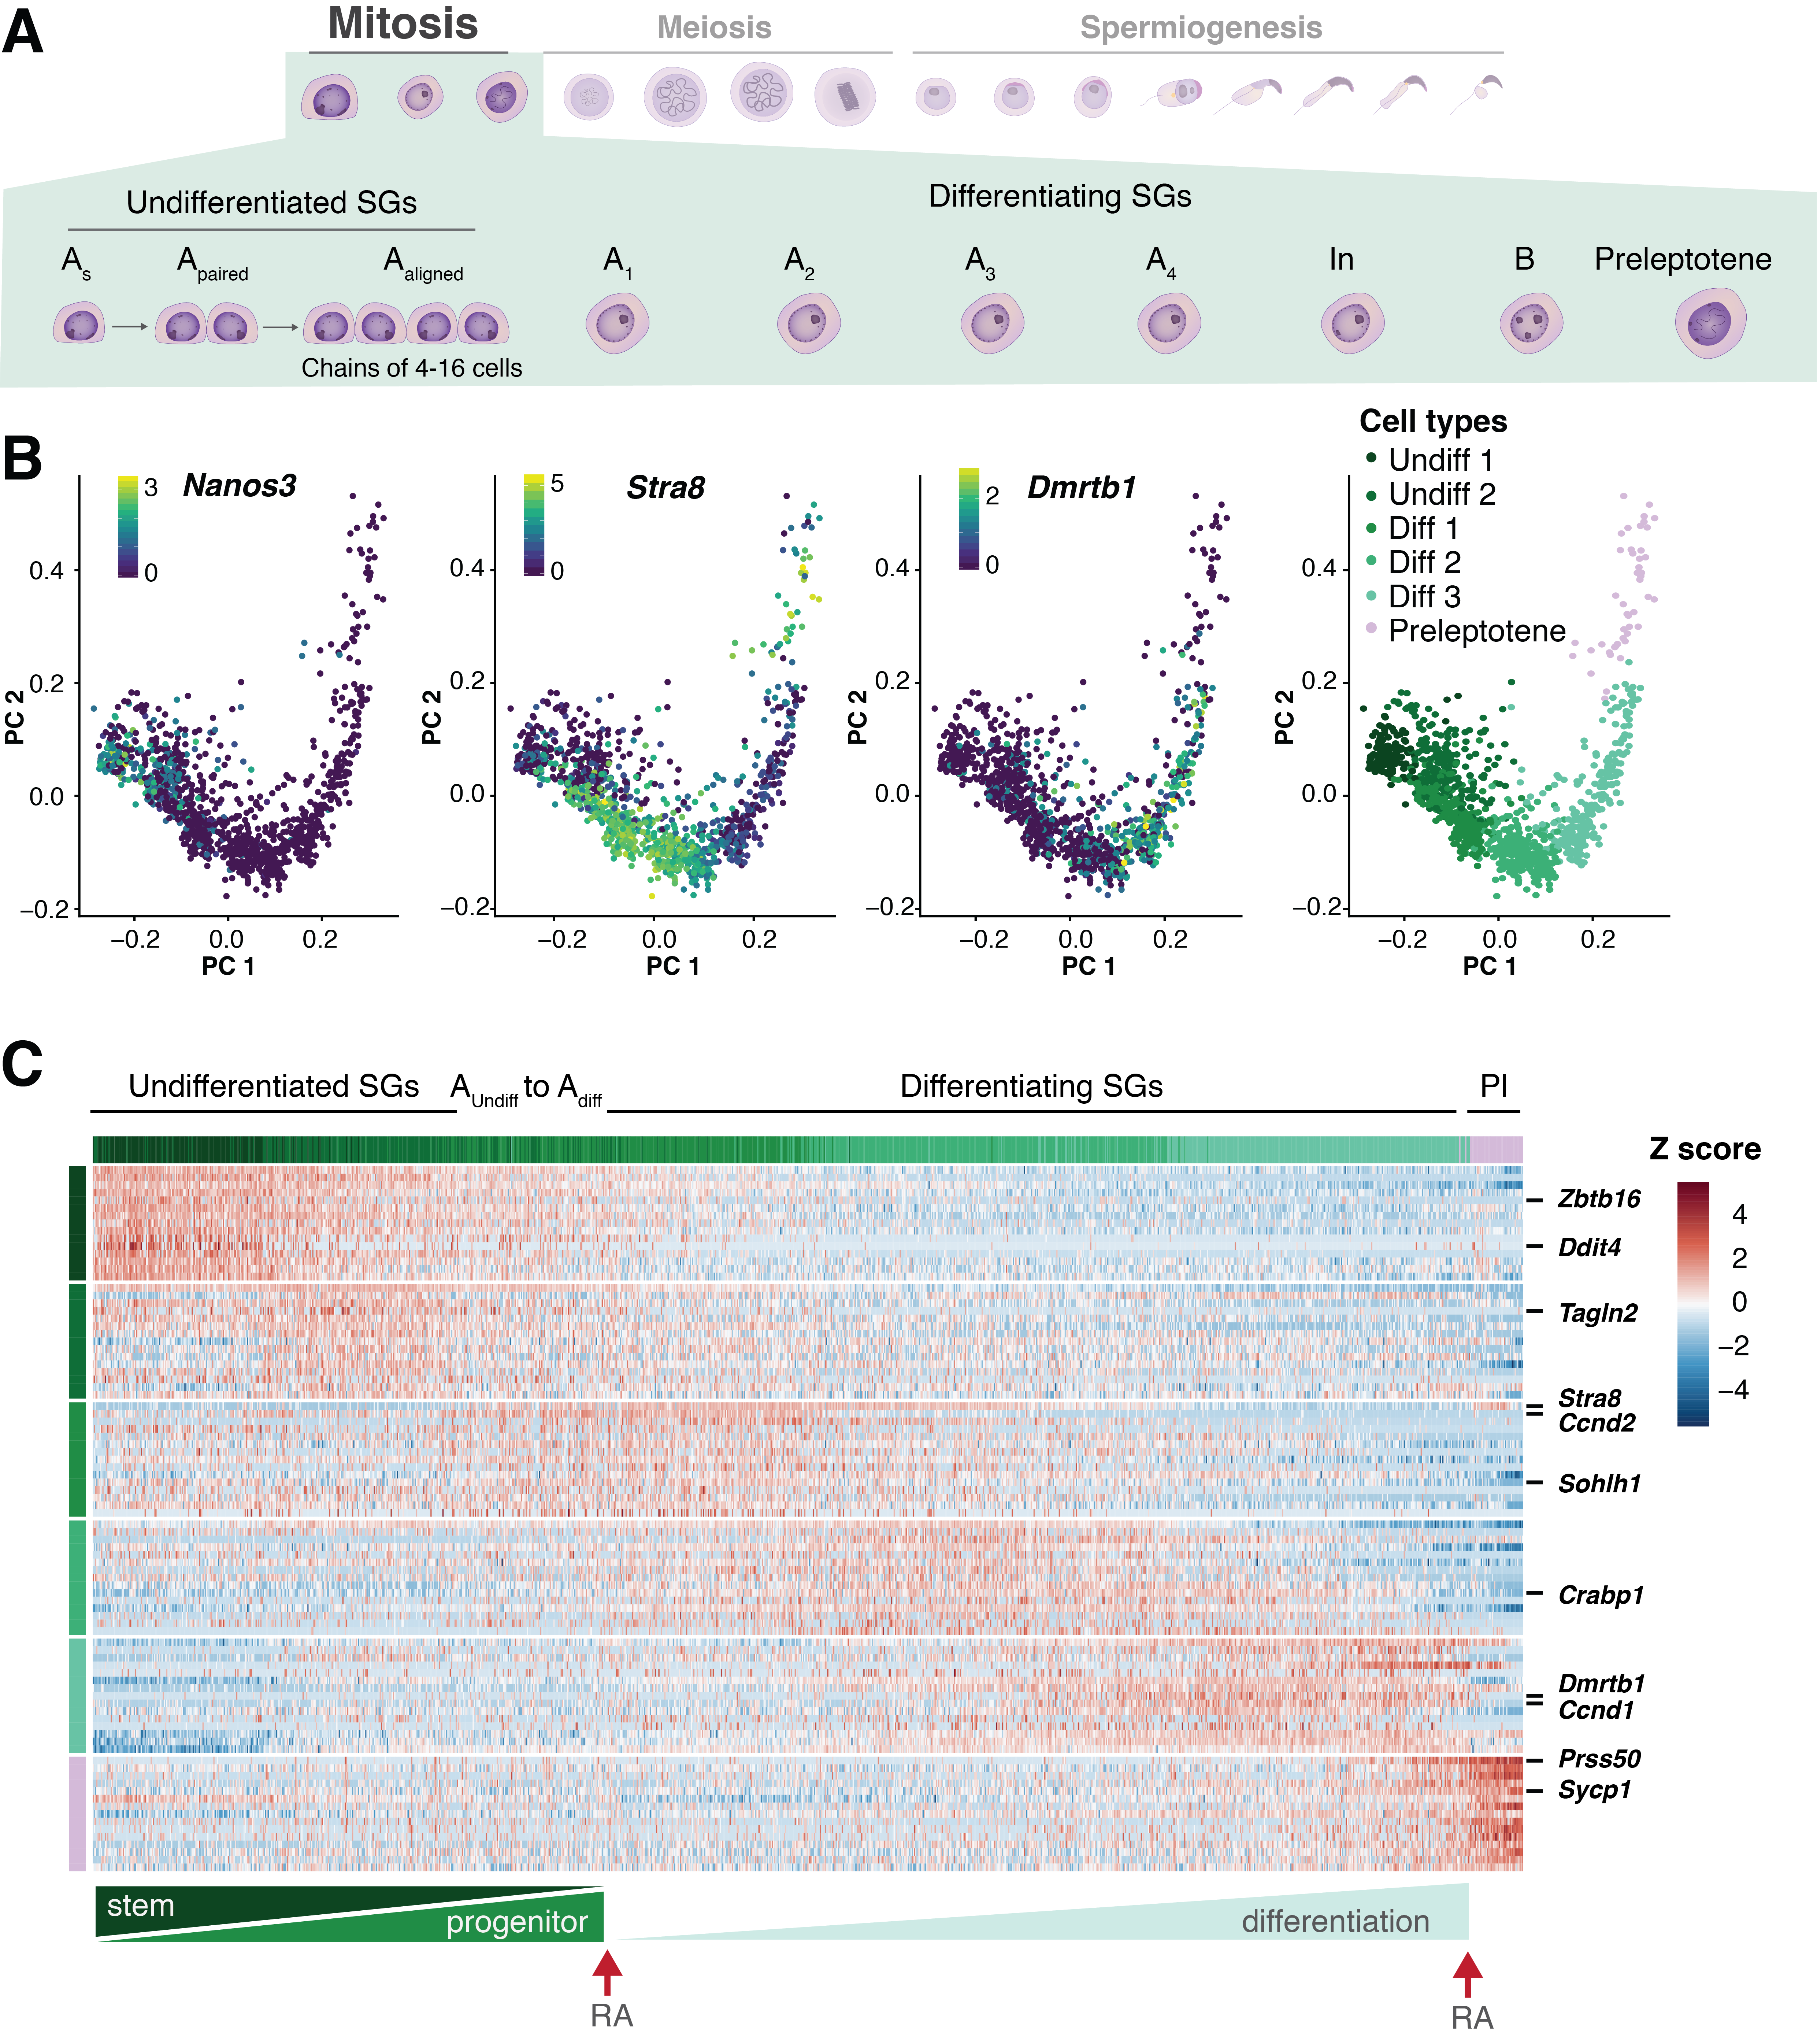
\includegraphics[width=\textwidth]{Fig_6.png}
\caption[DNA, epigenetic and translational features that modulate expression noise]{\textbf{DNA, epigenetic and translational features that modulate expression noise.}\\
Promoter sequence, number of transcription factor (TF) binding sites (TFBS, number of transcriptional start sites (TSS), enhance elements, RNA polymerase II (RNAPII) loading, DNA methylation, nucleosome positioning, histone modifications, polycomb repressive complex binding, miRNAs, nuclear export of mRNA, ribosome binding and blockage via stem loop formation are features that induce gene-specific intrinsic noise.}
\label{fig0:overview_intrinsic}
\end{figure}

\subsubsection{DNA features}

One of the key regulatory steps prior to RNA synthesis is the binding of \glspl{TF} to specific DNA sequences within the regulatory region of a gene which then triggers the controlled production of primary RNA transcripts from the DNA of this gene \citep{Latchman1993}. Mutations in the DNA sequence such as \glspl{SNV} can alter the binding affinity of TFs and therefore the rate at which a gene is expressed \textbf{(Fig.~\ref{fig0:DNA_features})}. A systematic study of the \textit{\gls{TDH3}} gene expression in yeast found that mutations in known \glspl{TFBS} decrease mean expression and increase expression noise. Moreover, Metzger \textit{et al.}, 2015 showed that evolutionary selection removes mutations that increase expression noise and that SNVs with large effects on expression noise show the lowest frequency within samples yeast strains \citep{Metzger2015}. \\

One of the most widely studied DNA motifs in relation to transcriptional noise is the TATA-box motif in promoters. Generally, TATA-box containing promoters show high levels of transcriptional noise \textbf{(Fig.~\ref{fig0:DNA_features})} \citep{Faure2017} possibly due to a simple activation cycle containing one or few inactive states \citep{Zoller2015}. Stress response genes are enriched for the TATA-box motif and allow an early adjustment to changing environmental conditions \citep{Lopez-Maury2009}. Moreover, TATA-box containing genes show an increased interspecies variability \citep{Tirosh2006} and higher spontaneous mutational variation \citep{Landry2007} indicating an increased evolvability of these particular genes. In an early study, Raser \textit{et al.}, 2004 studied the noisy expression controlled by the budding yeast \textit{\gls{PHO5}} promoter. This promoter contains the TATA-box motif and is has been shown that transcriptional noise is reduced when a mutational modification decreases the TATA-box strength \citep{Raser2004}. A more recent study confirmed this result and found mutations in yeast promoters that eliminate the TATA-box motif which resulted in reduced noise levels for these genes \citep{Hornung2012}. \\

A possible confounding factor for the increased noise of TATA-box containing promoters is the number of TFBSs. Tirosh \textit{et al.}, 2006 detected a two-fold enrichment of TBFSs in TATA-box containing promoters \citep{Tirosh2006}. A later study showed that transcriptional noise scales with increased numbers of TFBSs \textbf{(Fig.~\ref{fig0:DNA_features})} \citep{Sharon2014}. Furthermore, TATA-box containing genes lack enhancing histone marks and their increased variability in expression can therefore be explained by repressed chromatin \citep{Choi2008} (see \textbf{Section \ref{sec0:epigenetic}} ).  \\

Promoters can be classified based on their shape as narrow with few \glspl{TSS} that predominantly control tissue-specific gene expression and broad promoters with larger numbers of TSSs that control the expression of house keeping genes. Mutations that alter the shape of promoters increase transcriptional noise \citep{Schor2017a}. Furthermore, promoters with one or few TSS show higher levels of expression variability \textbf{(Fig.~\ref{fig0:DNA_features})} \citep{Faure2017}.\\

In addition to SNVs, \glspl{CNV} (usually defined as copy number variability of regions $\geq$ 1kb in comparison to a reference genome) in parts of the genome influence gene expression and contribute to, for example, schizophrenia and autism \citep{Gamazon2015}. Combined analysis of DNA and RNA has shown that genes with low copy number tend to be noisier expressed compared to genes with multiple copies \textbf{(Fig.~\ref{fig0:DNA_features})} \citep{Dey2015}. In the context of monoallelic expression, genes located on the X chromosome show increased mRNA half-life which in turn increases transcript stability reduces noise  to levels of autosomal genes \citep{Faure2017}.

\begin{figure}[!h]
\centering
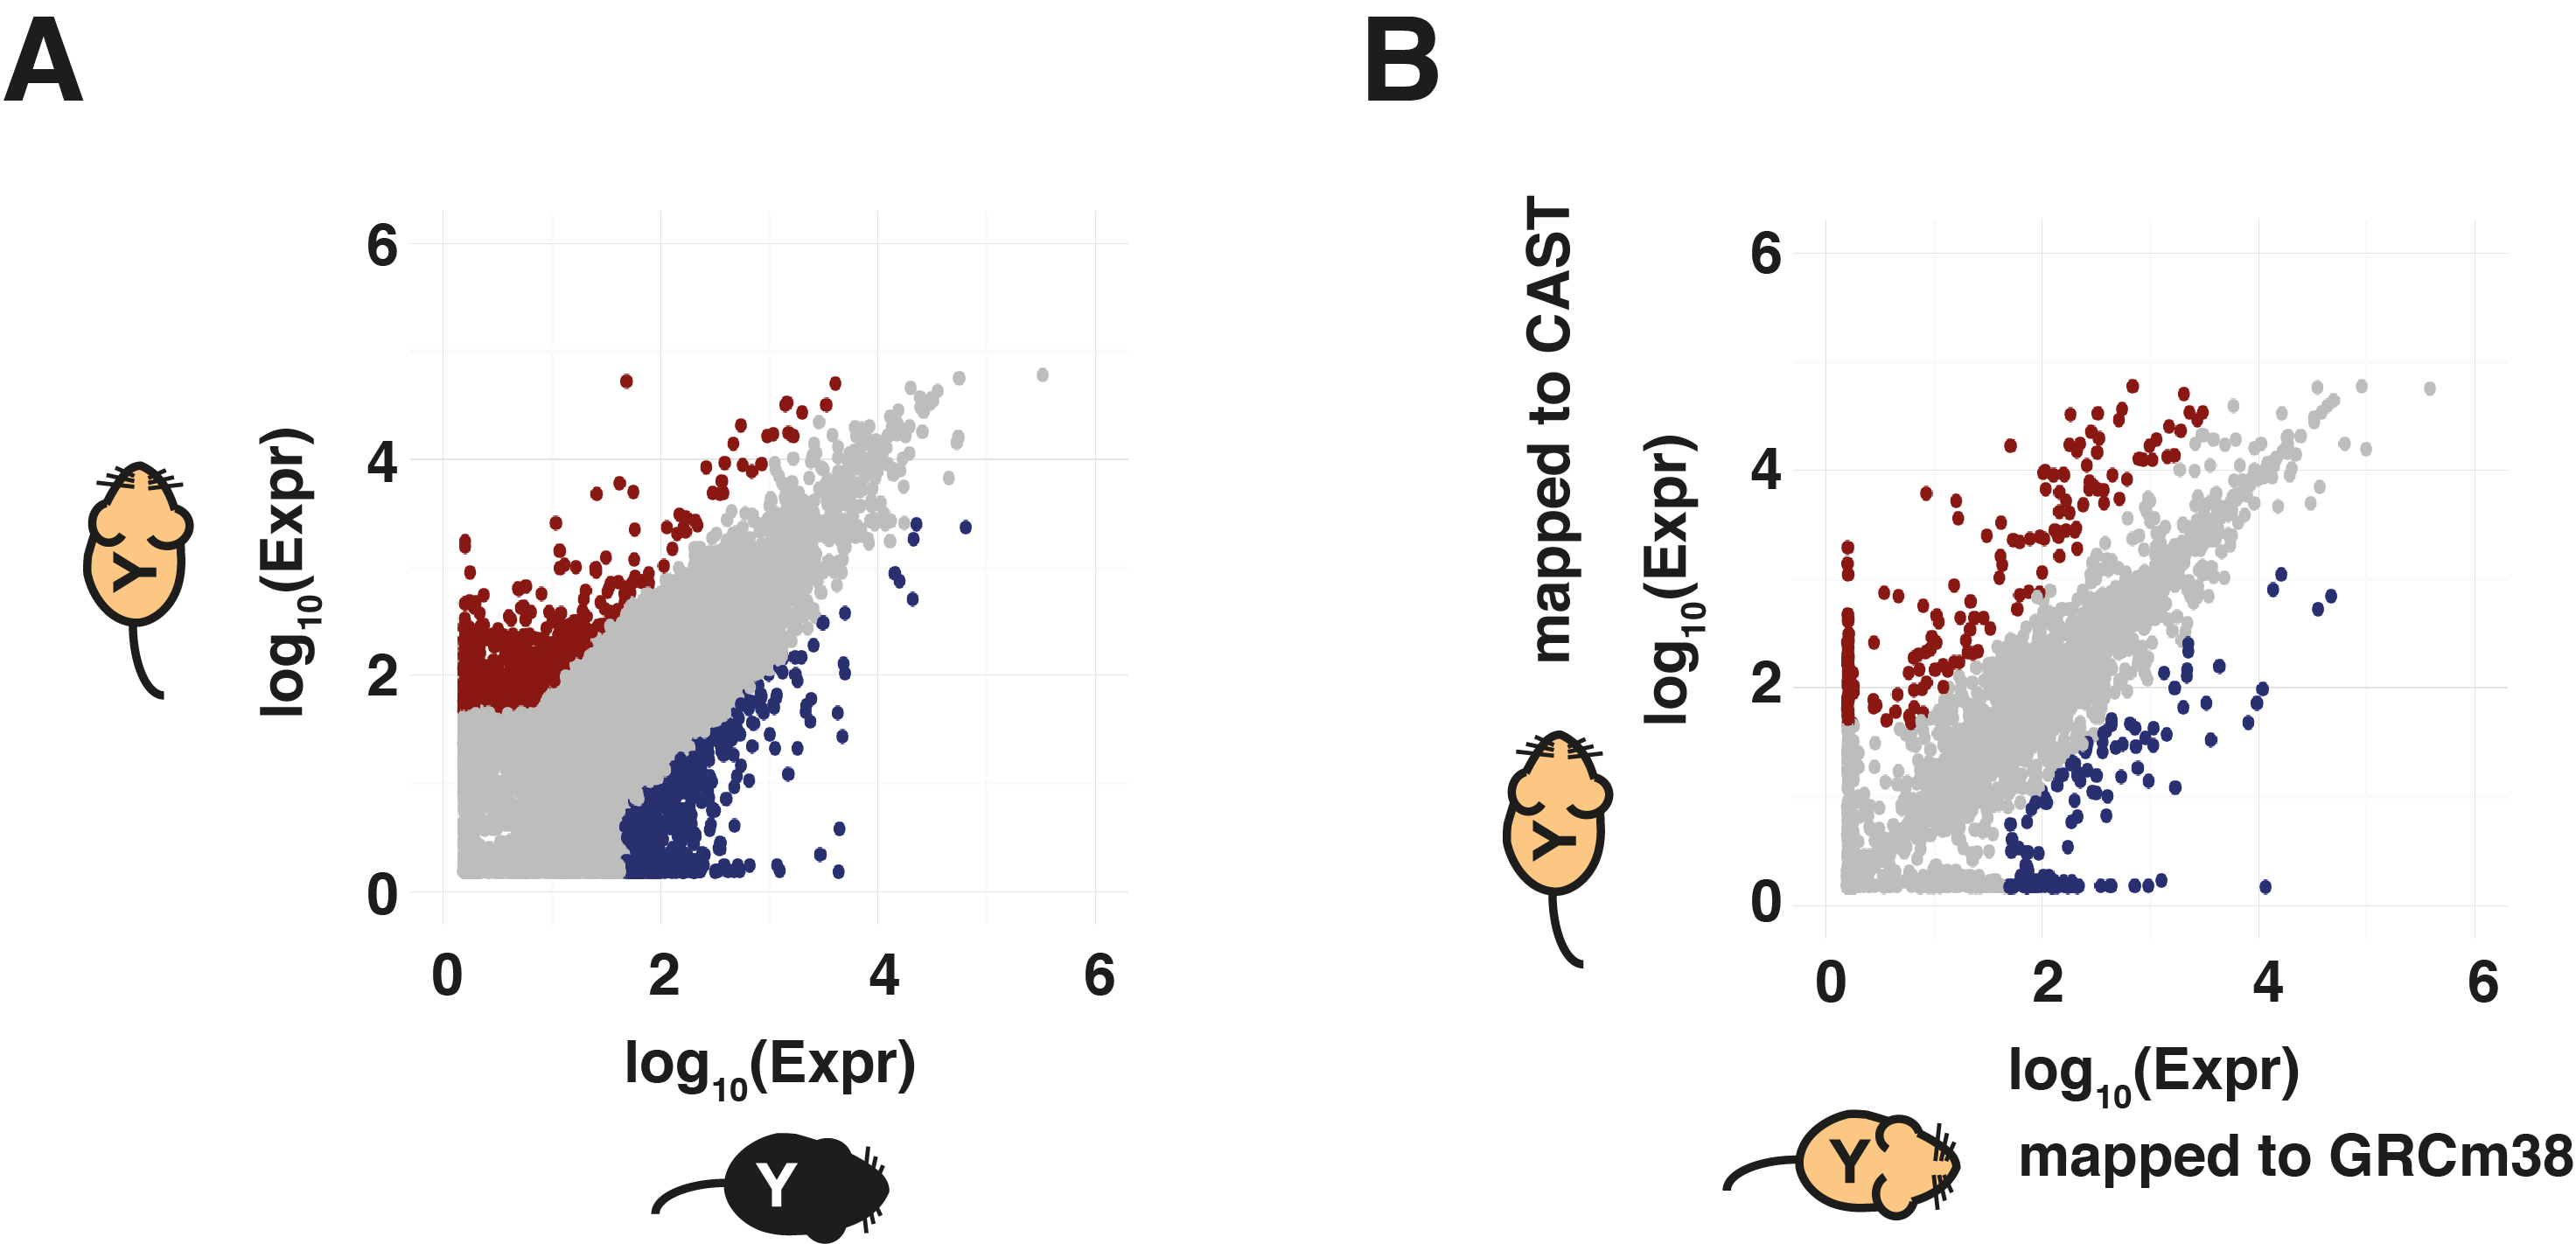
\includegraphics[width=0.85\textwidth]{Fig_7.png}
\caption[Features of the DNA sequence induce expression noise]{\textbf{Features of the DNA sequence induce expression noise.}\\
Mutations of the transcription factor (TF) binding site (TFBS), the presence of a TATA box, increase number of TFBSs, reduced number of transcriptional start sites (TSS) and reduced copy number of genes can induce transcriptional noise.}
\label{fig0:DNA_features}
\end{figure}

\subsubsection{Epigenetic factors}
\label{sec0:epigenetic}

Epigenetic factors are generally described as DNA methylation at \gls{CpG} dinucleotides, histone modifications and nucleosome positioning  \citep{Portela2010} and is defined as "the study of changes in gene function that are mitotically and/or meiotically heritable and that do not entail a change in DNA sequence" \citep{Wu2001}. \\

CpG islands are genomic sites of more than 200 bases with a GC content of more than 50\% where DNA methylation can preferentially occur. Methylation of CpG islands in promoters represses transcription while methylation in gene bodies facilitates transcription \citep{Portela2010}.  Recently, the presence of CpG islands in gene bodies but also at the TSS and in promoter regions was linked to a reduction in transcriptional noise \citep{Faure2017}. Similarly, previous findings showed that expression noise scales negatively with gene body methylation \cite{Huh2013}. Morgan and Marioni, 2018 studied the effect of CpG island size on transcriptional noise using scRNA-Seq data. Genes associated with short CpG island promoters tend to be noisier expressed than genes with long CpG island promoters. Furthermore, early response genes during \gls{LPS} stimulation of bone-marrow derived dendritic cells and heregulin stimulation of human breast cancer cells are enriched for those with short CpG island promoters \citep{Morgan2018}. \\

Modifications of histones induce the activation or repression of chromatin and  therefore indirectly modulate gene expression\citep{Suganuma2011}. In an extensive study to link histone modifications to transcriptional noise, Faure \textit{et al.}, 2017 detected several histone modifications in promoter/core promoter motifs, at the TSS and in gene bodies to increase or decrease noise. The repressive \gls{H3K27me3} mark is linked to higher noise levels when present at the TSS, in promoters and in gene bodies. The enhancer related \gls{H3K4me1} mark only increases noise when present at the TSS and in the core promoter sequence while the repressive \gls{H3K9me3} mark increases noise when present in the promoter motif. The activating marks \Gls{H3K4me3}, \gls{H3K9ac} and \gls{H3K36me3} are linked to low levels of noise when present in gene bodies. In addition to these single features, bivalent promoters that carry the repressive \gls{H3K27me3} and enhancing \gls{H3K4me3} marks show high levels of transcriptional noise \citep{Faure2017}.\\ 

Polycomp repressive complexes (PRCs) are epigenetic modifiers of histones to repress transcription of developmental genes \citep{Chittock2017}. They can bind together with active \gls{RNAPII} to bivalent promoters and switching between the repressed and active states introduces gene expression variability across a population of cells \cite{Kar2017}. Additionally, deletions of different histone deacetylation complexes (Set3C and Rpd3(L)), that both repressed transcription by removing H3K9ac, showed different effects on transcriptional bursting \citep{Weinberger2012}.  Confirming this, a later study showed that gene body and promoter histone modifications independently influence burst size and burst frequency and therefore regulate mean expression and noise in an uncoupled fashion \cite{Wu2017}. These results indicate a fine-tuned regulation of transcriptional noise and support the functional role of biological noise in cell populations.\\

Chromatin is the packaged state of DNA within the nucleus and its central element are nucleosomes. Nucleosomes are made up of eight of the four histones (H3, H4, H2A, H2B) and 147 bases of DNA can wrap around this complex. An array of histone modifying enzymes exits that regulate the opening or closing of the chromatin; termed heterochromatin and euchromatin respectively \citep{Kouzarides2007}. Tirosh \textit{et al.}, 2008 showed that promoters with high nucleosome occupancy close to the TSS tend to display a high range of expression levels across varying conditions (transcriptional plasticity). Distant nucleosome-rich regions are on the other hand associated with low transcriptional noise \citep{Tirosh2008}. Nucleosome covered promoters display shorter transcriptional rates, which in turn explains increased transcriptional noise for these promoters \cite{Dey2015}. Single-cell measures indicate cell-to-cell variations in nucleosome positioning around the \textit{PHO5} promoter upon stress induction. Even in the non-stressed state, a small fraction of cells exhibit nucleosome free regions at the promoter which explains low and possibly noisy expression of \textit{PHO5} \citep{Small2014}. Deletion of chromatin remodeling complexes that remove nucleosomes upon transcription factor binding results in increased transcriptional noise compared to wild-type cells \citep{Raser2004}. \\ 

Boundaries between heterochromatin and euchromatin are controlled by boundary elements, such as the transcription factor \Gls{CTCF}, that recruit chromatin modifying factors \citep{Kouzarides2007}. CTCF also regulates transcription by activating or repressing promoters and regulates distant chromatin interactions \citep{Kim2015a}. Recent studies suggest that long-range enhancer-promoter interactions modulate transcriptional noise. Interference of CTCF-mediated enhancer-promoter contact either by CTCF knock-out or CTCF-binding site deletion leads to increased expression variability in selected genes \citep{Ren2017}. Enhancers are cis-regulatory elements, non-coding DNA with TFBSs, that regulate the expression of neighbouring genes \citep{Blackwood1998}. Genes within super-enhancer loci, a region with multiple enhancers, controlling pluripotency master regulators show high levels of variability in expression and down-stream targets of these master regulators show similar co-variation across mESCs \citep{Faure2017}.\\

Moreover, the positioning of genes on the genome controls expression noise with densely clustered genes being less noisy expressed in comparison to non-clustered genes \citep{Kustatscher2017}. Additionally, genes positioned next to “noisy” genes display higher levels of transcriptional variability compared to genes that are located in proximity to “stable” genes \citep{Kar2017}. Expression noise is also increased for genes that are located in a repressed neighborhood, namely active genes in constitutive nuclear lamina-associated domains \citep{Faure2017}.\\

\textbf{Table \ref{tab0:epigenetic}} summarises the relation between epigenetic features and noisy gene expression.

\begin{table}[hb	]
\centering
\caption{Epigenetic control of transcriptional noise}
\label{tab0:epigenetic}
\begin{tabular}{l l c c}
\toprule
\toprule
 & Feature & Noisy & Stable \\ 
\midrule
\midrule
\multirow{3}{*}[-2pt]{DNA methylation} & CpG islands &  & \checkmark{} \\
\cmidrule{2-4}
& Short CpG islands & \checkmark{} &  \\
\cmidrule{2-4}
& Gene body methylation &  & \checkmark{} \\
\midrule
\multirow{7}{*}[-2pt]{Histone modification} & H3K27me3 (TSS, promoter, gene body) & \checkmark{}  & \\
\cmidrule{2-4}
& H3K4me1 (TSS, promoter) & \checkmark{}  & \\
\cmidrule{2-4}
& H3K9me3 (promoter) & \checkmark{}  & \\
\cmidrule{2-4}
& H3K4me3 (gene bodies) &  & \checkmark{}\\
\cmidrule{2-4}
& H3K9ac (gene bodies) &  & \checkmark{} \\
\cmidrule{2-4}
& H3K36me3 (gene bodies) &  & \checkmark{} \\
\cmidrule{2-4}
& H3K27me3 and H3K4me3 & \checkmark{}  & \\
\midrule
\multirow{3}{*}[-2pt]{Nucleosome position} & Nucleosome rich promoters & \checkmark{} & \\
\cmidrule{2-4}
& Distant nucleosome rich regions &  & \checkmark{} \\
\cmidrule{2-4}
& Deletion of nucleosome remodelling complexes & \checkmark{}  & \\
\midrule
\multirow{7}{*}[-2pt]{Genome architecture} & CTCF knock-out & \checkmark{} & \\
\cmidrule{2-4}
& CTCF binding site depletion & \checkmark{} & \\
\cmidrule{2-4}
& Clustered genes &  & \checkmark{} \\
\cmidrule{2-4}
& Nuclear-lamina associated genes & \checkmark{} & \\
\bottomrule
\bottomrule
\end{tabular}
\end{table} 

\newpage

\subsubsection{Transcriptional features}

Transcription is initiated by TFs binding to specific regulatory DNA sequences followed by recruitment of RNAPII, RNA synthesis and RNA degradation. As discussed above, promoter architecture, namely the location and accessibility of TFBS and RNAPII binding sites, dictates mean expression and transcriptional noise. \\

In bacteria, the intracellular physical distance between TF source and the promoter sequence influences expression variability. TF expression proximal to their target genes results in less noisy expression compared to regulator sources distant to the promoter sequence \citep{Goni-Moreno2017}. Once TFs bind to their target sequence, Carey \emph{et al.}, 2013 showed that mean expression to noise ratio is promoter dependent while in the majority of cases, noise negatively scales with mean expression \citep{Carey2013}. \\

Similar to TF binding dynamics, the assembly of RNAPII complexes modulates transcriptional noise. An early study identified the connection between paused RNAPII and synchronous expression of target genes. Genes without pre-loaded RNAPII show more stochastic activation patterns \citep{Boettiger2009}. This finding has later been confirmed using scRNA-Seq data while increased variability was detected for genes with non-pause RNAPII across the full range of expression levels \citep{Day2016}.\\

\begin{figure}[!h]
\centering
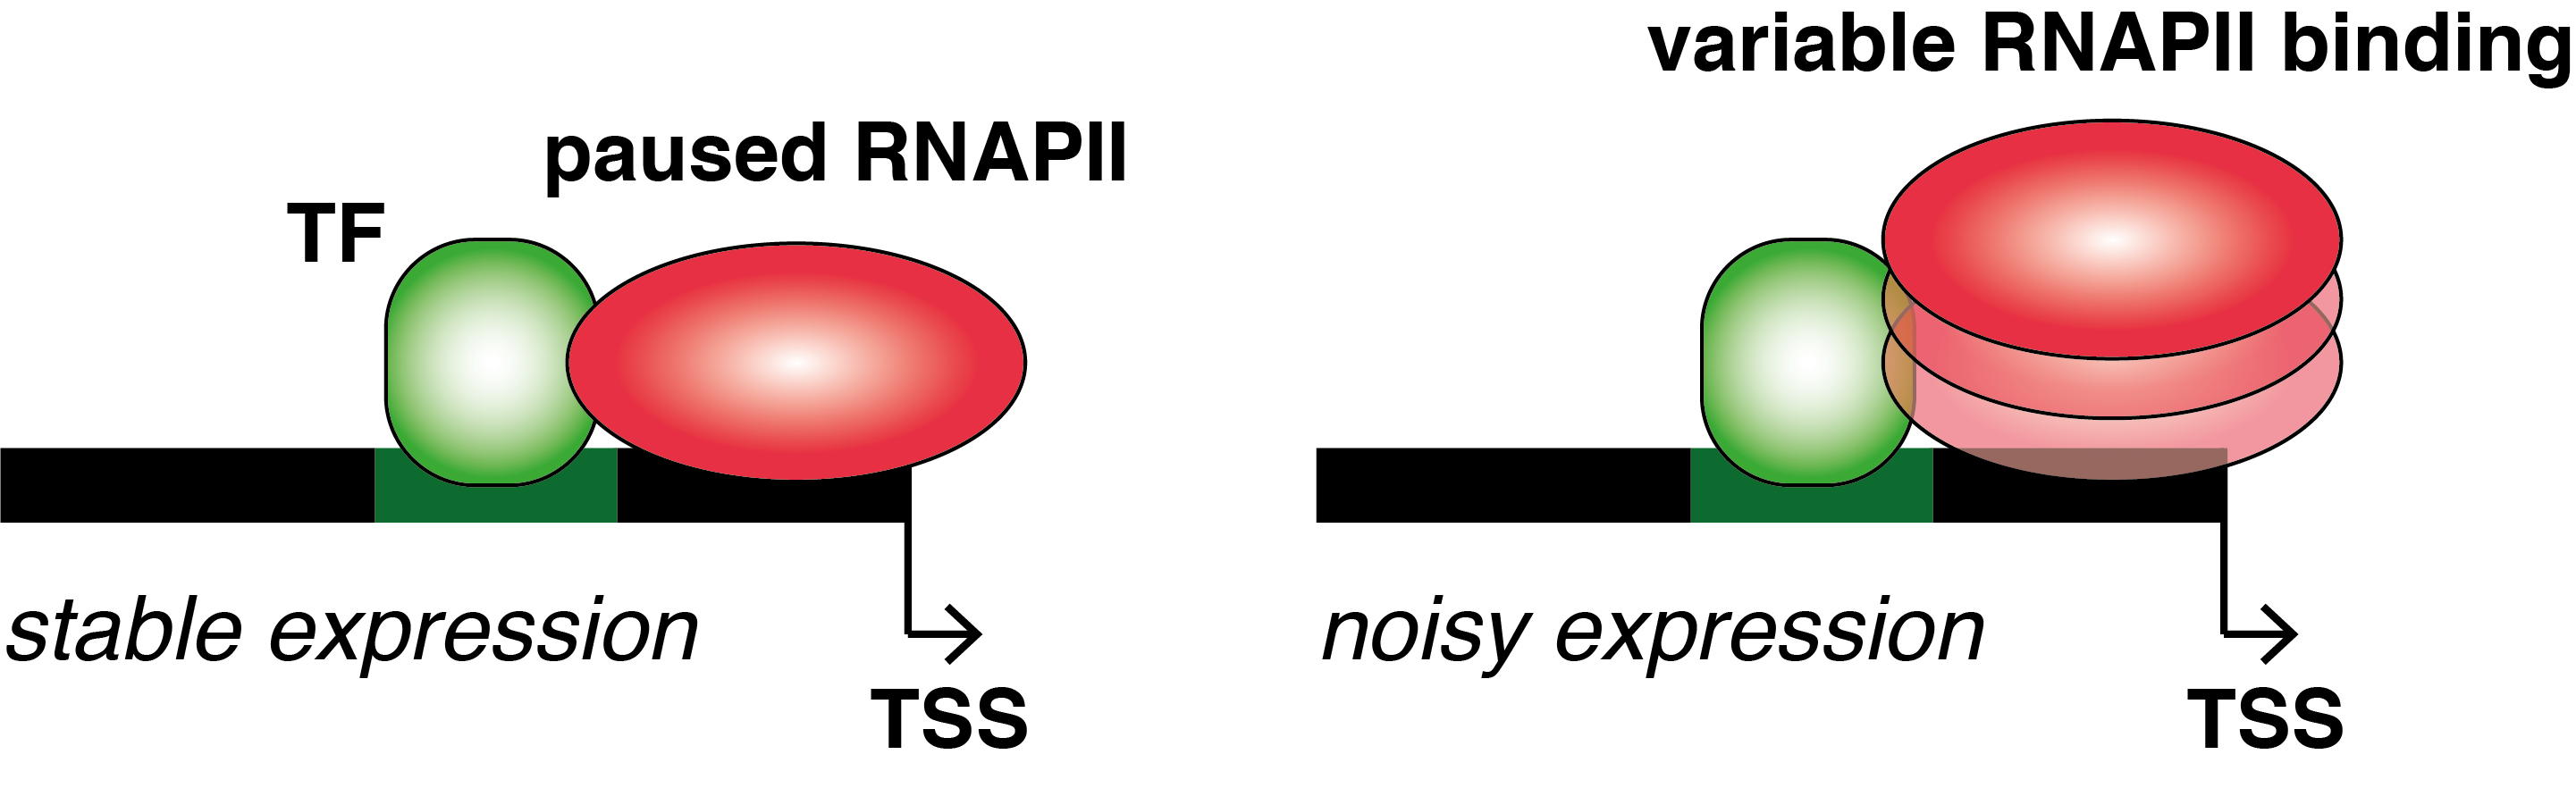
\includegraphics[width=0.7\textwidth]{Fig_8.png}
\caption[RNAPII pausing reduces transcriptional noise]{\textbf{RNAPII pausing reduces transcriptional noise.}\\
Left: Pre-loaded RNA polymerase II (RNAPII) allows direct transcription upon transcription factor (TF) binding. Right: RNAPII recruitment induces gene expression variability.}
\label{fig0:DNA_features}
\end{figure} 

\newpage

\subsubsection{Post-transcriptional and translational features}

After synthesis, pre-RNAs are polyadenylated and spliced to form mRNA that relocates from the nucleus to the cytoplasm where translation occurs to synthesise proteins \cite{Glisovic2008}. On the post-transcriptional and translational level, mRNA localization, structure, degradation and translation have been shown to influence cell-to-cell variations in protein abundance.

Upon transcriptional activation, RNAs are produced in burst-like patterns while burst frequency modulates mean expression and noise, and burst size influences solely mean expression \citep{Hornung2012}. While bursty transcript synthesis introduces stochastic fluctuations in nuclei between cells, active export of mRNAs into the cytoplasm can dampen this source of variability \citep{Battich2015a}. Reduces cytoplasmatic noise has also been shown for two nuclearly retained genes in the mammalian liver. Furthermore, this mode of noise control was proposed to be active across a range of metabolic tissues \cite{BaharHalpern2015a}.\\

\begin{figure}[!h]
\centering
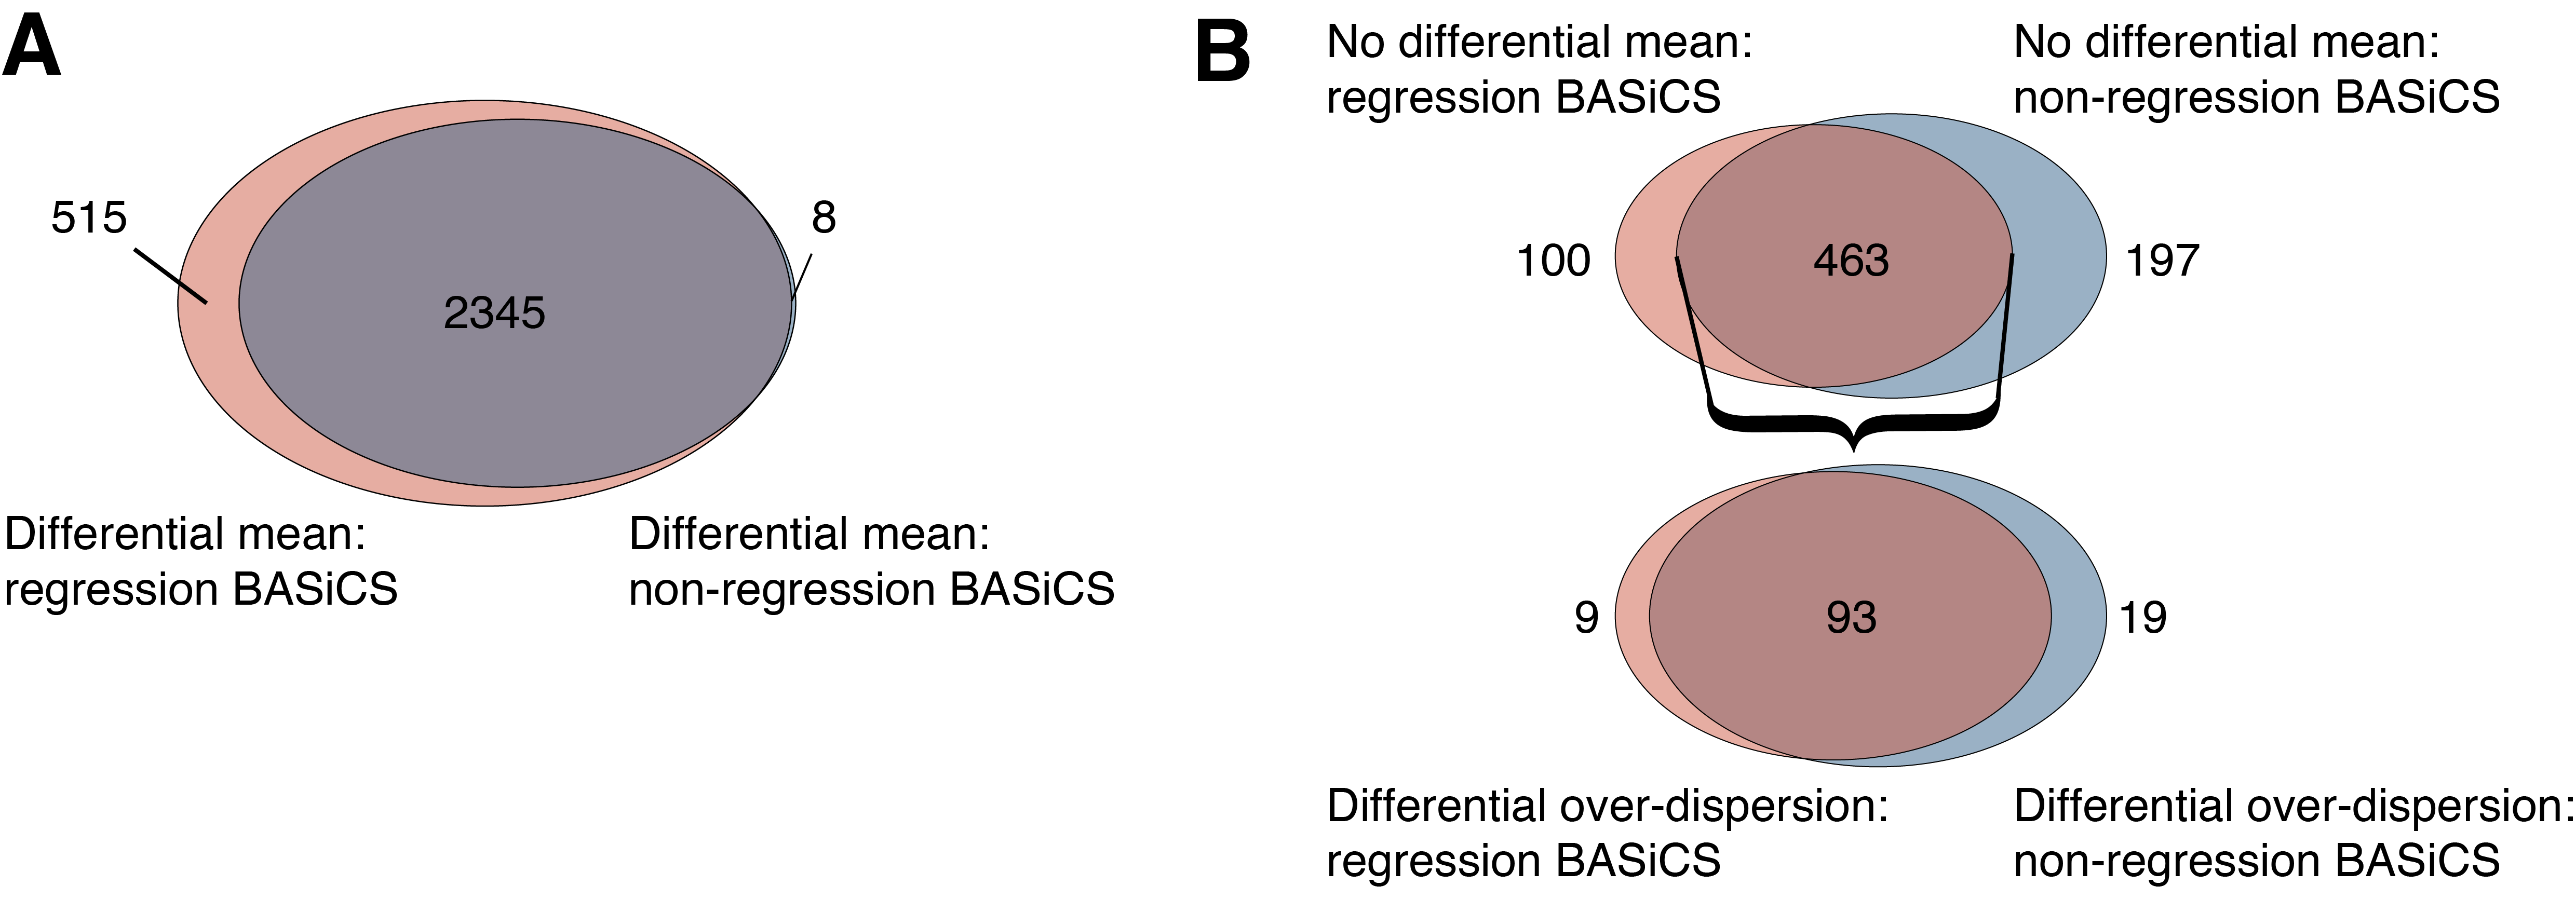
\includegraphics[width=\textwidth]{Fig_9.png}
\caption[Post-transcriptional regulation to control noisy expression]{\textbf{Post-transcriptional regulation to control noisy expression.}\\
Bursty expression introduces nuclear variation in transcript abundance that is buffered due to retention at the nuclear membrane. Within the cytoplasm, micro RNAs degrade lowly expressed genes to reduce expression noise. Deletion of the ribsosome binding site as well as stem loop formation increase variability in protein abundance across cells. Arrows indicate either increased (red) or decreased noise (green) dependent on the regulatory mechanism.}
\label{fig0:DNA_features}
\end{figure} 

\newpage

Within the cytoplasm, mRNAs are subject to translation or degradation. At this stage, stochasticity from bursty gene expression is propagated to variation in protein abundance. The availability of mRNAs for translation is not only dictated by their syntheses but also their degradation rate. mRNA degradation is accelerated by recognition of micro RNAs. This process has been shown to preferentially reduce noise levels for lowly expressed genes in mESCs to possibly retain cellular identity \citep{Schmiedel2015}. Similarly, temporal averaging of long-lived transcripts reduces noise in mRNA abundance. In that way, increased transcript stability compensates for noise introduced by the single-allele expression of genes on chromosome X \citep{Faure2017}.  \\

In addition to noise introduced by stochastic processes on the transcriptional level, the recognition and binding of ribosomes to mRNAs for translation initiation features a source for variations in protein abundance. Modulating translational efficiency by mutating the ribosome binding site and initiation codon showed an interaction between translation and variation in protein abundance \citep{Ozbudak2002}. Additionally, mRNA secondary structure formed by stem loops and ploy(G) motifs affects translation initiation and increases noise in protein levels \citep{Dacheux2017a}.

\subsection{Extrinsic noise}

Extrinsic noise within a cell population arises from cells being in different regulatory states. Here, differences in cellular components introduce variation in mRNA and protein abundance. Examples for cell states in otherwise homogeneous populations are characterized by differences in metabolism, cell cycle, volume, cell-to-cell and environmental signalling as well as cell density. It has been shown that extrinsic noise forms a major contribution to variations in gene expression and that transcript distributions can be predicted from the cellular state, population context and microenvironment \citep{Battich2015a}.

\subsubsection{Cell cycle}

Cell cycle has been widely discussed to form a crucial source of extrinsic noise \citep{Colman-Lerner2005a, Newman2006}). In yeast populations, differences in transcriptional activities between the G1 and S/G2/M phases of the cell cycle lead to large-scale transcriptional heterogeneity across cell populations \citep{Zopf2013}. Under nutrient-poor conditions, growth rate is reduced and noise is elevated due to cells being in different cell-cycle stages \citep{Keren2015}.  Even under optimal growth conditions for mESCs (2i media), cell cycle related genes show strong heterogeneity in expression across the cell population \citep{Kolodziejczyk2015cell}. Nonetheless, sorting cells into similar cell cycle stages did not drastically reduce noise levels \citep{Raser2004}. When quantifying cell-to-cell variation, cell cycle induced extrinsic noise is often seen as unwanted variation and can mask more subtle transcriptional heterogeneity. Computational methods have been developed to correct for this confounding effect to enhance the underlying noise signal \citep{Buettner2015, Buettner2017}. 

\subsubsection{Cell volume}

Cellular volume provides another explanation for global differences in mRNA content between individual cells introducing large-scale transcriptional heterogeneity. Even though cell volume changes during cell cycle progression, within each phase cell volume varied as much as across all phases. It has been shown that mRNA counts scale with cellular volume to maintain transcript concentrations within each cell \citep{Kempe2015, Padovan-Merhar2015, Zhurinsky2010}. To avoid this source of heterogeneity, normalization approaches correct for differences in mRNA content between individual cells \citep{Vallejos2017}.

\subsubsection{Metabolism}

The effect of metabolic fluctuations has been studied in \textit{E. coli} populations. Variations in biochemical reactions are induced by noise in the expression of their corresponding catalytic enzymes. Changes in metabolism are then coupled to varying growth rates of individual cells, which in turn introduces large-scale transcriptional heterogeneity in cell populations \citep{Kiviet2014}.  

\subsubsection{Expression capacity}

Fluctuations in the expression capacity of cells due to quantitative differences in RNAPII or ribosomes induce global variability among the majority of proteins \citep{Colman-Lerner2005a}.

\subsubsection{Cell signalling}

A different source of extrinsic noise is the intra- or inter-cellular signalling state of individual cells. Fluctuations in membrane bound or cytoplasmic proteins lead to inconsistent transmission of signalling stimuli as exemplified by variability in TRAIL-induced apoptosis \citep{Spencer2009}. Similarly, variations of regulators in the \gls{ERK} signalling pathway introduce downstream variability in nuclear response. The degree of which nuclear ERK response is varied depends on the position of the regulator in the topology of the signalling pathway \citep{Iwamoto2016}. In \textit{C. elegans}, perturbation of the Wnt signalling pathway displayed different degrees of variability in expression of the key Hox gene for Q neuroblast migration, \textit{mab-5}. It has been proposed that extrinsic noise, in this case the strength of the Wnt signal, modulates intrinsic variation in the expression of \textit{mab-5} \citep{Ji2013}. 

\subsubsection{Physical constrains}

Physical constrains on cell growth and the direct population context influence the state of individual cells \citep{Battich2015a}. Snijder \textit{et al.}, 2009 performed detailed imaging based analysis of adherent human cells that were infected with different viruses. Clathrin mediated endocytosis was most variable with low cell density leading to inefficient mouse hepatits virus infection. Dengue virus preferentially infects edge cells while simian virus 40 infection was decreased with large cell density \citep{Snijder2009}. These experiments indicate the importance of local cellular microenvironment and cell-cell contacts leading to heterogeneity in cell states. 


\newpage
%!TEX root = ../intro.tex
%******************************
%	 Quantification of biological noise
%*****************************

\section{Quantification of cell population heterogeneity} 

To quantify biological noise in cellular systems, single-cell approaches employ either sequencing or imaging technologies to extract genomic, transcriptomic, epigenetic or proteomic features from individual cells. These technologies show specific advantages and limitations on the level of throughput and content. 
In this section, I will discuss the applicability of single-cell sequencing and imaging technologies as a potential read-out for cell population heterogeneity induced by transcriptional noise.

\subsection{Single-cell sequencing}

Next generation sequencing approaches have been applied to individual cells to quantify variation in DNA sequence, mRNA expression, epigenetic marks and protein abundance within a cell population. 

\subsubsection{Single-cell whole genome sequencing}

\Gls{scDNA-Seq} has previously been used to identify CNVs and SNVs between single cells \citep{Zong2012}. 
Based on these read-outs, tumour heterogeneity and evolution \citep{Navin2011} as well as lineage relationships in the human brain were inferred \citep{Evrony2015}. 
To obtain enough genomic material, \gls{WGA} is performed on DNA from individual cells. The \gls{SCOMP} degrades DNA via restriction enzymes, includes a primary \gls{PCR} amplification step and a later re-amplification via comparative genomic hybridisation \citep{Klein1999}. \Gls{MDA} is based on the random initiation of amplification via oligonucleotide primers with strand displacement \citep{Dean2002}. Compared to MDA, \gls{MALBAC} achieves an initial quasi-linear amplification step by pre-amplification using primers with handle sequences. 
Full amplicons form hairpins that are exponentially amplified prior to sequencing \citep{Zong2012}. \\

The main limitation of single-cell DNA sequencing is the genomic coverage per cell. 
While the detection of SNVs requires deep sequencing of individual cells, CNVs can be detected with shallow sequencing therefore allowing the throughput to increase \textbf{(Fig.~\ref{fig0:scDNA-Seq})} \citep{Knouse2016, Baslan2015}. 
Recently, Vitak \emph{et al.}, 2017 introduced \gls{sci-Seq} which allows the generation of thousands of single-cell genomes for sequencing. 
In the first step, multiple nuclei are sorted into each well of a 96 well plate and the genomic DNA is labelled with barcodes by transposase tagging. 
In the second step, 15-25 tagged cells are sorted into individual wells of a PCR plate where the second round of barcoding is performed during amplification. In that way, CNVs of over 15,000 cells can be assessed \citep{Vitak2017}.

\begin{figure}[!h]
\centering
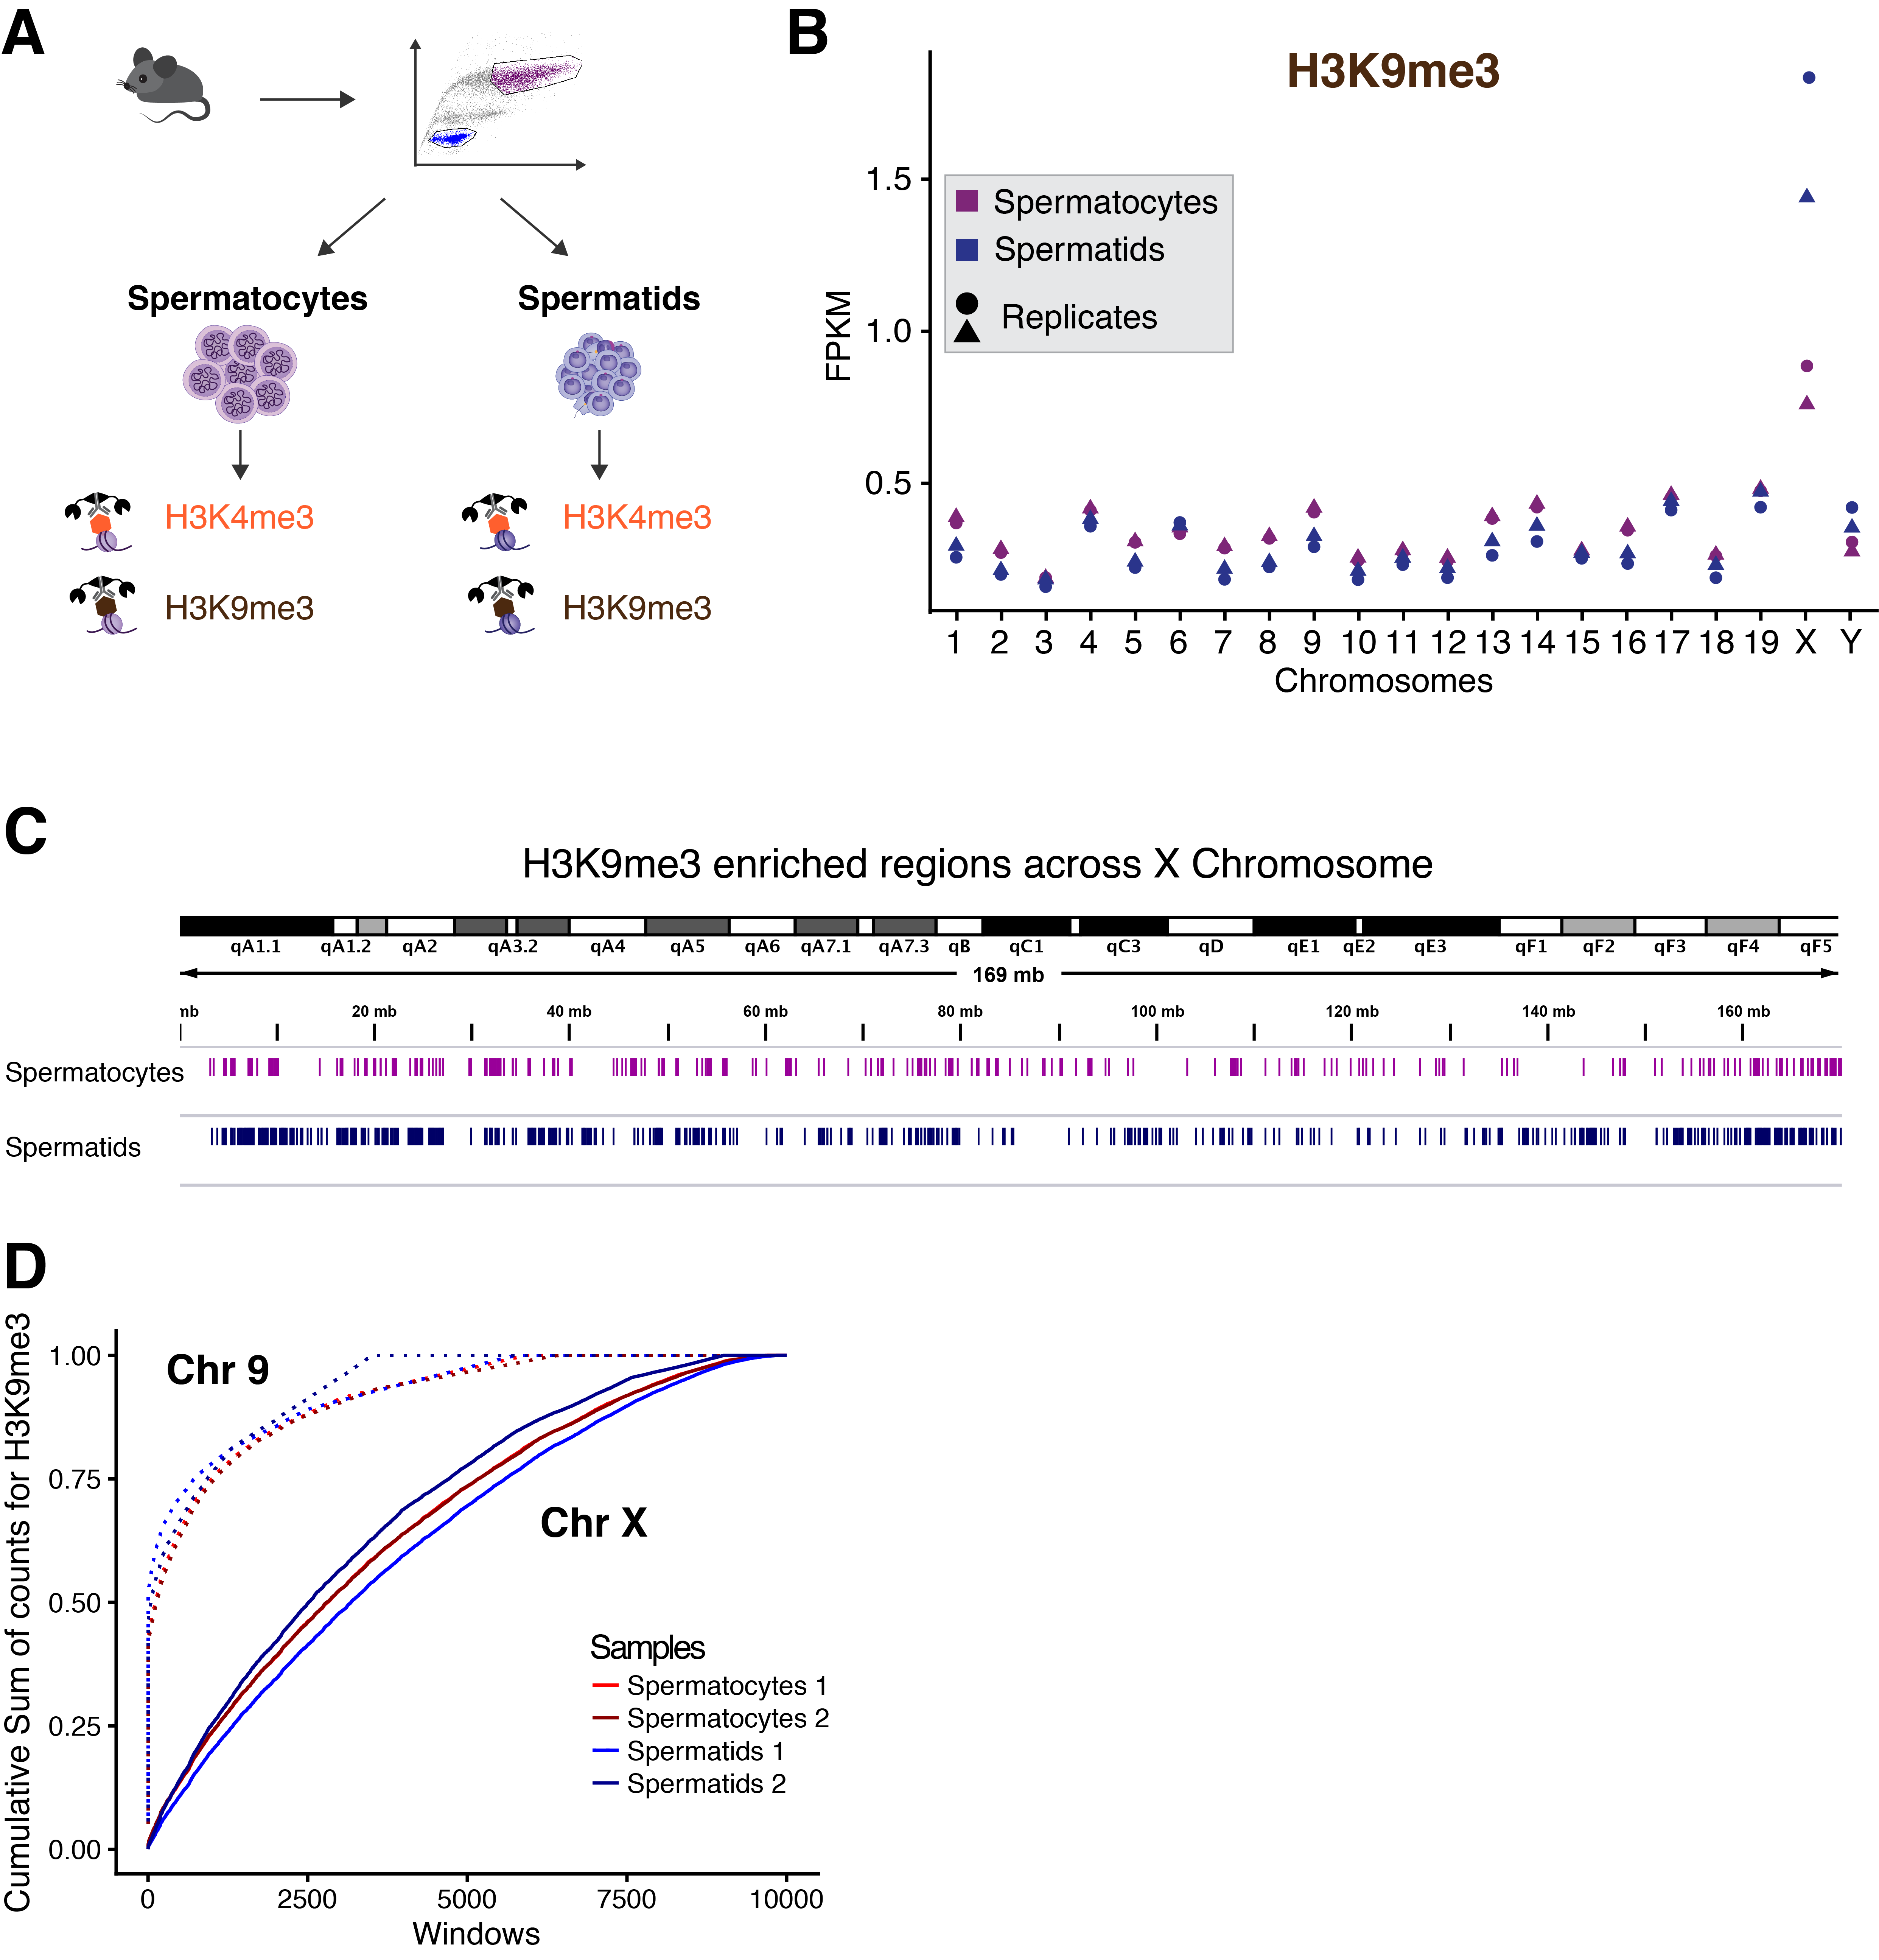
\includegraphics[width=\textwidth]{Fig_12.png}
\caption[ScDNA-Seq allows detection of SNVs and CNVs between individual cells]{\textbf{ScDNA-Seq allows detection of SNVs and CNVs between individual cells.}\\
Individual nuclei are captured in 96-well plates and directly lysed or fixated for multiplexing. Whole genome amplification (WGA) can be performed using MDA, MALBAC or SCOMP resulting in amplified genome segments. 
Depending on the biological question, whole genomes are either sequenced thoroughly to detect single nucleotide variants (SNVs) while shallow sequencing can be used to detect copy number variations (CNVs).}
\label{fig0:scDNA-Seq}
\end{figure}

\vspace{-5mm}

\subsubsection{Single-cell RNA sequencing}

Initial approaches to quantify mRNA abundance within single cells included targeted microfluidic-based single-cell \gls{RT-PCR} \citep{Warren2006} and whole-transcriptome read-outs of hand-picked cells \citep{Tang2009}. 
Methods for cell capture range from micromanipulation \citep{Grindberg2014} and laser capture microdissection \citep{Frumkin2008} as targeted methods with low throughput to  \gls{FACS} \citep{Hayashi2010, Dalerba2011, Jaitin2014}, microfluidics \citep{Trapnell2014, Treutlein2014} and microdroplets \citep{Klein2015, Macosko2015} as high-throughput approaches \textbf{(Fig.~\ref{fig0:scRNA-Seq})}. 
More broadly, microfluidic-based \gls{scRNA-Seq} approaches can be grouped into valve-, droplet- or well-based strategies \citep{Prakadan2017}. \\

A variety of scRNA-Seq protocols have been published that utilise different methods for mRNA \gls{RT}, \gls{cDNA} amplification and library preparation. 
All of these commonly used techniques for scRNA-Seq select and reverse transcribe mRNA (poly(A) tailing). 
The initial protocol introduced by Tang \textit{et al}, 2009 \citep{Tang2009} was improved by incorporating a template switching mechanism at the 5' end of the mRNA thus reducing the 3' sequencing bias present in previous methods \citep{Islam2011} (see below and \textbf{Fig.~\ref{fig0:scRNA-Seq}}). 
This \gls{STRT} method shows 5' bias in read mapping and was later modified for full-length transcript detection (SmartSeq \citep{Ramskold2012} and SmartSeq2 \citep{Picelli2013}). 
CEL-Seq \citep{Hashimshony2012} and CEL-Seq2 \citep{Hashimshony2016} use \gls{IVT} to linearly amplify cDNA prior to sequencing as opposed to exponential amplification in other techniques. 
Protocols for sequencing library preparation have been optimised for Illumina, SOLiD or PacBio sequencing \citep{Kolodziejczyk2015review}. \\

During scRNA-Seq, minute amounts of mRNA are captured and amplified generating a high degree of technical noise, which distorts quantification of true biological variability. 
To account for this, a set of external RNAs developed by the \gls{ERCC} \citep{Rna2005} can be added to the cell lysate. 
Based on the reads mapped to ERCC spike-ins, technical noise can be removed from total expression variability \citep{Brennecke2013, Vallejos2015BASiCS}. 
Another way to reduce noise derived from amplification biases in scRNA-Seq experiments is to tag each mRNA molecule with a \gls{UMI} \citep{Kivioja2011, Islam2014}.\\

One example of a commercially available platform that captures individual cells and performs lysis, reverse transcription and pre-amplification of cDNA is the Fluidigm\textsuperscript{\textregistered{}} C1 system. 
Individual cells are loaded into \glspl{IFC}, also termed "chips", that allows capturing of 96 to 800 cells. 
Depending on the size of the cells, this system offers chips with different capture well sizes. 
Each well can be microscopically inspected to differentiate between empty capture sites and single cells \citep{Kolodziejczyk2015review}. 
The C1 system uses the SMARTer\textsuperscript{\textregistered{}} chemistry to capture poly(A) mRNA with modified oligo(dT) primer. 
Next, the \gls{RTase} reverse transcribes from the 3' to the 5' end of the mRNA and adds non-templated deoxycytidines to the 3' end of the cDNA. The template-switch primer contains guanosines at its 3' end that base-pair with the deoxycytidines on the cDNA to create an extended template. 
The \gls{RTase} extends to the end of the template-switch primer. 
This produces single-stranded cDNA that contains the SMARTer tag sequence, the 3' end of the mRNA, the full-length transcript up to the 5' end of the mRNA, and the reverse complement of the SMARTer tag sequence. 
Amplification of this cDNA is performed by PCR on the chip \cite{Fluidigm2015}. After pre-amplification, the cDNA is collected and prepared for sequencing.\\

In parallel to extending scRNA-Seq protocols to robustly capture mRNA transcripts, efforts have been made to increase the throughput of this technology. 
Jaitin \emph{et al.}, 2014 introduced \gls{MARS-Seq} to sequence over 4000 cells of the mouse spleen. 
MARS-Seq captures cells in 384 well plates and labels transcripts of each cell with a combination of 2 random barcodes. 
This multiplexing strategy is performed using a liquid handling robot and cells can be pooled for sequencing library preparation which reduces costs and time effort \citep{Jaitin2014}. 
The first large-scale technique that captured tens of thousands of cells was introduced by Fan \emph{et al.} in 2015. 
Here, 10,000 cells were captured in a 100,000 microwell surface. 
Additionally, barcoded beads were loaded into the surface until saturation. 
This Cyto-Seq approach is similar to the more recent Seq-Well technology \citep{Gierahn2017}. 
Each bead is coated with barcodes containing a unique sequence, a bead-specific barcode, a UMI and a oligo(dT) primer. After cell lysis and mRNA capture, beads are pooled and cDNA synthesis can be performed prior to sequencing \citep{Fan2015}. 
In the same year, the inDrop and Drop-Seq technologies were introduced \citep{Klein2015, Macosko2015}. 
Both technologies use microfluidic platforms to merge droplets containing barcodes, lysis and reverse transcription reagents with droplets containing cells. 
Similar to the above described Cyto-Seq \citep{Fan2015}, after lysis and mRNA capture, droplets are pooled for sequencing. 
The main difference is that cell-specific barcodes in Drop-Seq are bound to beads and to a polyacrylamide mesh in inDrop.  

\begin{figure}[!h]
\centering
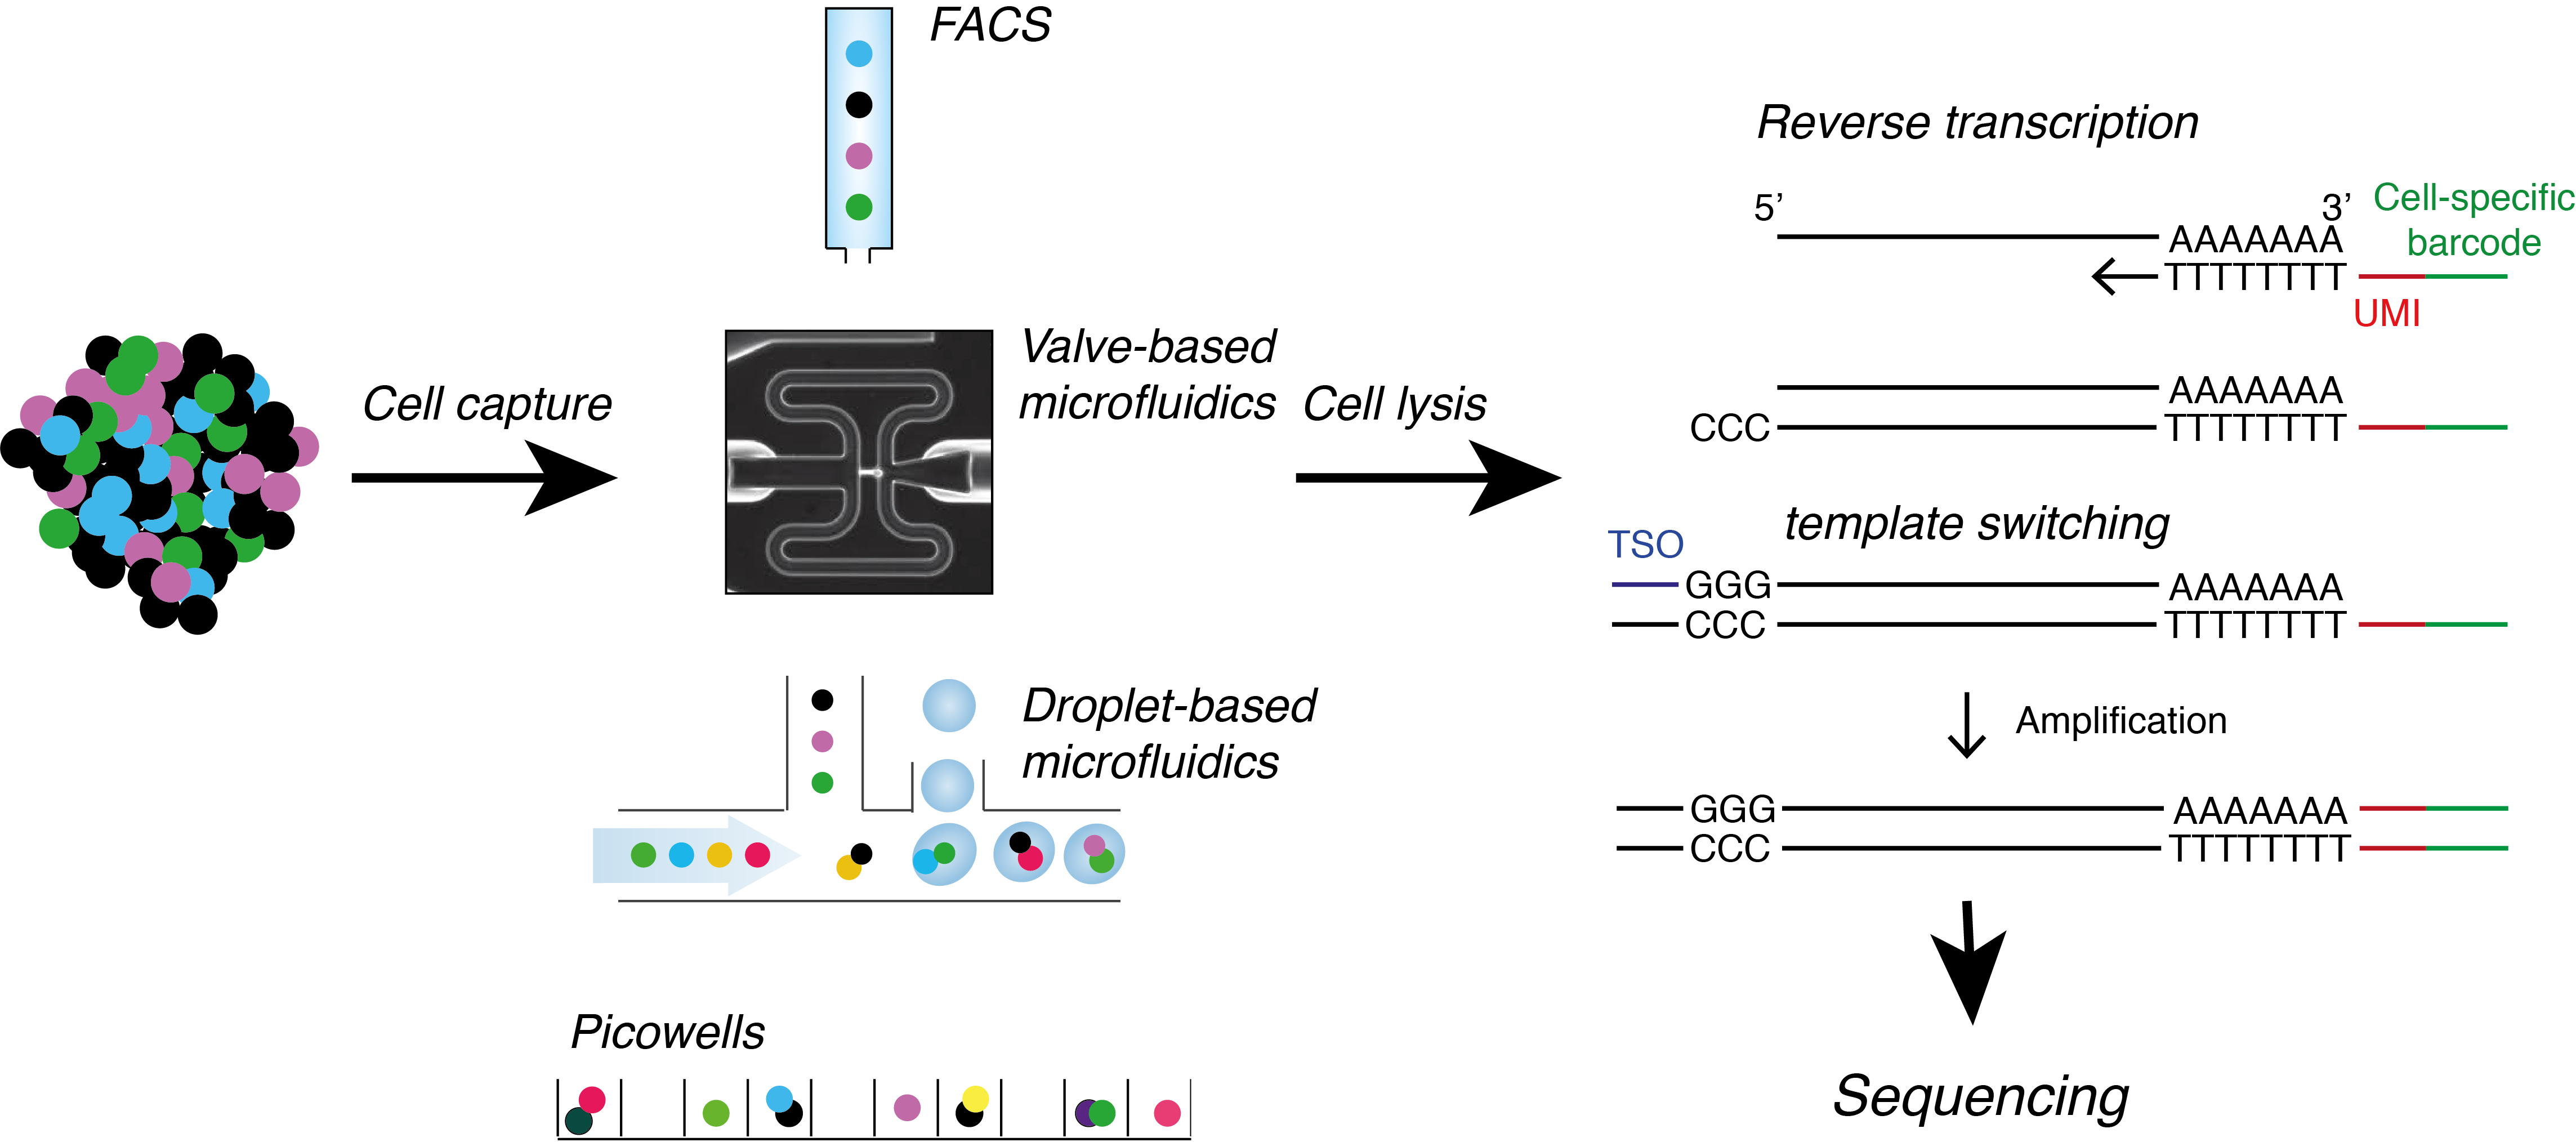
\includegraphics[width=0.9\textwidth]{Fig_13.png}
\caption[Workflow for scRNA-Seq technologies]{\textbf{Workflow for scRNA-Seq technologies.}\\
Single cell suspensions are obtained by tissue dissection and dissociation. 
Commonly used cell capture technologies include fluorescence-activated cell sorting (FACS), valve-based microfluidics (Fluidigm\textsuperscript{\textregistered{}} C1 system), droplet-based microfluidics (10X Genomics\textsuperscript{\textregistered{}} system), or picowells. 
After cell capture and lysis, poly(dT) oligos capture mRNA prior to reverse transcription. 
In the case of droplet-based cell capture, poly(dT) oligos are tagged with a unique molecular identifier (UMI) and a cell-specific barcode. 
\Gls{RT} generates cDNA from the template RNA. One strategy for RT is the template-switching protocol where the reverse transcriptase adds three cytidines at the 5' end of the template. 
A \gls{TSO} binds to the cytidines and allows amplification from the 5' end. 
After cDNA amplification, libraries are prepared for sequencing. For this, transposase degrades full length transcripts and Illumina sequencing primers are added (C1 system). 
In the case of the 10X Genomics system, the first read has been added next to the cell-specific barcode while the second read is added after cDNA fragmentation. This protocol shows a 3' bias.}
\label{fig0:scRNA-Seq}
\end{figure}

\newpage

10X Genomics\texttrademark{} has introduced a platform that uses these concepts to generate hundreds of thousands of \gls{GEM}. 
Around 80\% of generated oil droplets capture barcoded gel beads in 8 channels in parallel. 
Each barcode consists of a sequencing adapter and primer, a 14bp sequence from a pool of 750,000 barcodes, a 10bp UMI and a 30bp poly(dT) oligotide to capture poly(A) mRNA \citep{Zheng2017}. 
GEMs are fused with individual cells at a low concentration and cell lysis begins instantaneously. 
mRNA molecules are captured by the poly(dT) barcode and enzymes needed for \gls{RT} are released from the gel beads. 
After RT, each cDNA contains a transcript-specific UMI and a GEM-specific barcode making demultiplexing possible \textbf{(Fig.~\ref{fig0:scRNA-Seq})}. 
Barcoded cDNA is pooled for PCR amplification and library preparation \citep{Zheng2017}.\\

Methods that even further increased the throughput of scRNA-Seq include \gls{SPLiT-Seq} and sci-RNA-Seq. Similar to sci-DNA-Seq (see above) these technologies are based on combinatorial indexing of mRNA in fixed cells or nuclei. 
Sci-RNA-Seq tags transcripts during two rounds of indexing with UMIs and a combination of two cell specific barcodes \citep{Cao2017}.  
SPLiT-Seq on the other hand performs transcript tagging during 4 cycles adding 4 barcodes \citep{Rosenberg2018}. 
In that way, around 1 million cells can be uniquely labelled. At this stage the limiting factor is the sequencing depth needed to obtain high-resolution whole transcriptomes of each cell.	
These approaches as well as the recently developed \gls{DroNc-Seq} also allow sequencing mRNA from nuclei which is the preferred method for clinical samples, archived materials, and tissues that cannot be readily dissociated \citep{Habib2017}. 


\subsubsection{Single-cell epigenomics}

Single-cell epigenomic methods capture the chromatin state, histone modifications and DNA methylation state of individual cells and allow quantification of epigenetic variability across a population of cells \textbf{(Fig.~\ref{fig0:scEpigenomics})} \citep{Clark2016}. 
To observe methylation states of CpG motifs, \gls{scBS-Seq} involves the extraction of genomic DNA and cytosine to uracil bisulfite conversion prior to library preparation. 
5-methylcytosine remains intact during conversion \citep{Smallwood2014, Farlik2015}. 
The throughput of this approach was scaled up by combinatorial indexing of fixed nuclei similar to sci-DNA-Seq (i) prior to bisulfite conversion and (ii) during PCR amplification (sci-MET-Seq) \citep{Basque2017}. 
\Gls{scRRBS-Seq} enzymatically digests genomic DNA prior to bisulfite conversion. 
CpG-rich fragments can be enriched and amplified via ligated adapters before high-throughput sequencing \citep{Guo2013}. 
Extending the read-out of scBS-Seq and scRRBS-Seq, \gls{sc5hmC-Seq} captures the first oxidative product of CpG sites towards de-methylation and therefore cellular variation of methylation dynamics. 
Instead of bisulfite conversion, 5hmC sites are glucosylated before enzymatic digestion and adapter ligation \citep{Mooijman2016}. \\

To measure histone modifications or transcription factor binding dynamics at the single-cell level, digested chromatin from individual cells is tagged with barcodes prior to \gls{IP} during \gls{scChIP-Seq} \textbf{(Fig.~\ref{fig0:scEpigenomics})}. 
With this droplet-based method, variable chromatin signatures were detected across a population of ESCs based on the \gls{H3K4me2} \citep{Rotem2015}. 

\begin{figure}[!h]
\centering
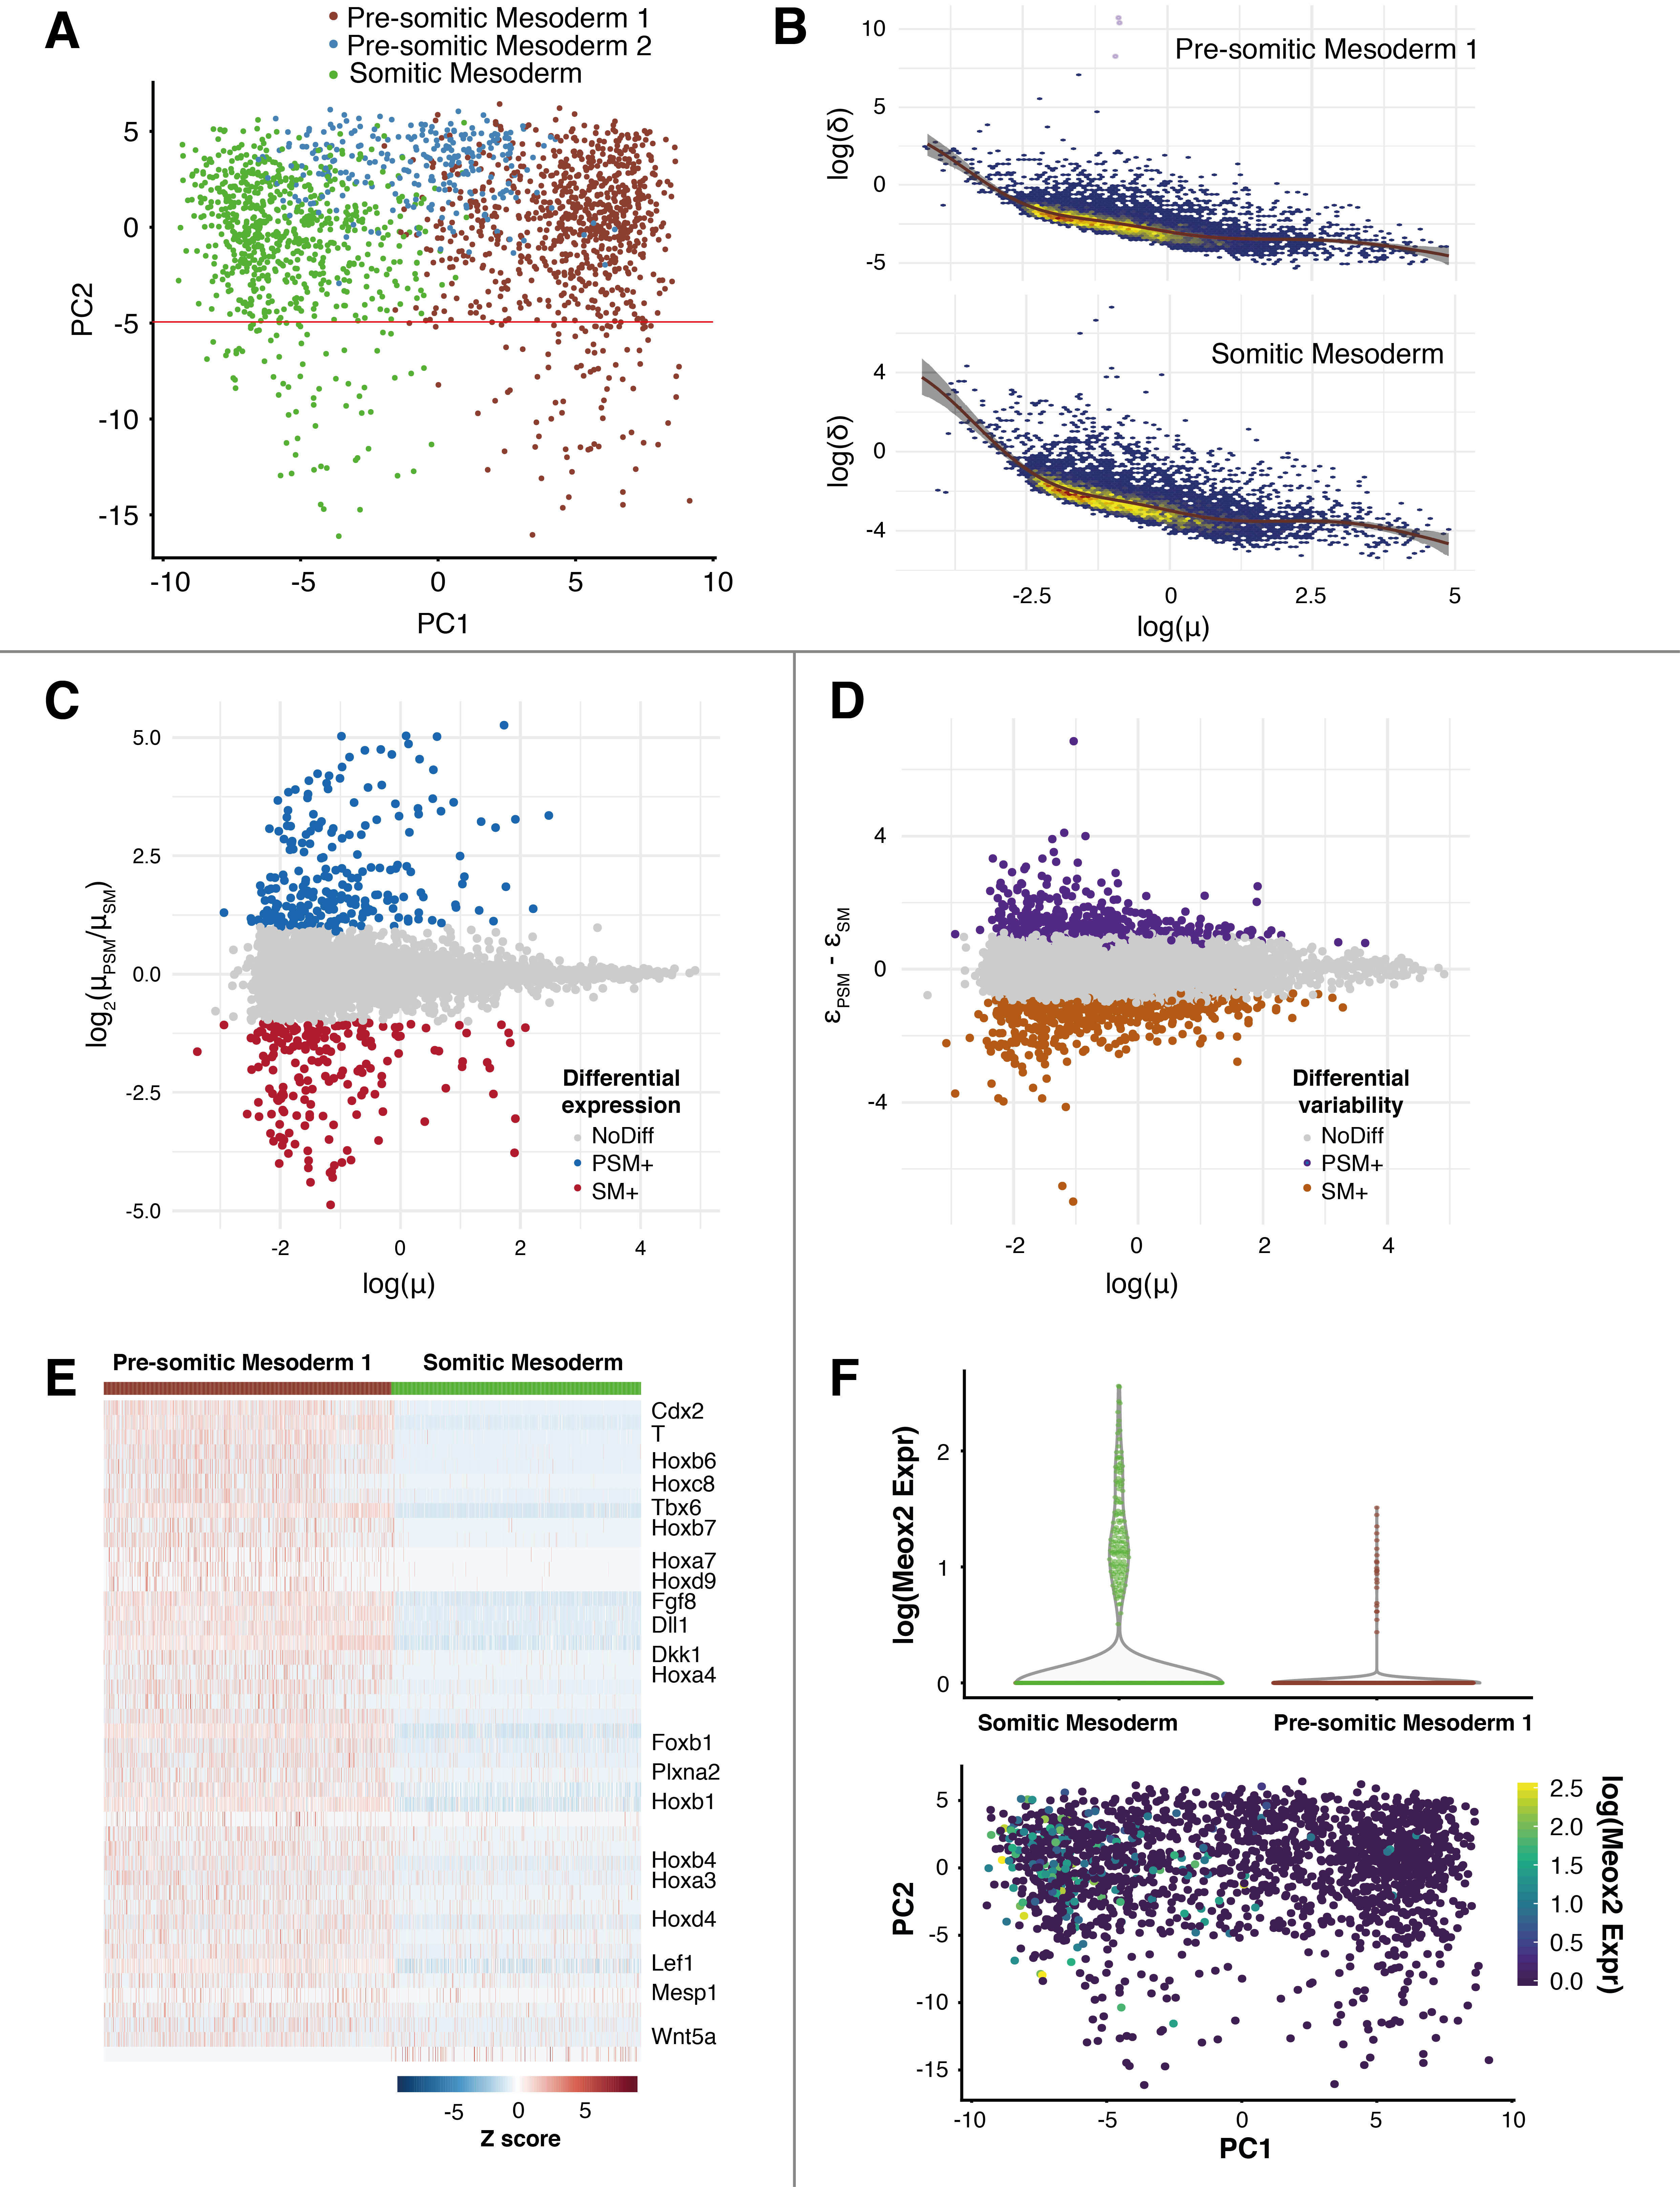
\includegraphics[width=\textwidth]{Fig_14.png}
\caption[Single-cell epigenomics to study chromatin structure and modifications]{\textbf{Single-cell epigenomics to study chromatin structure and modifications.}\\
Single-cell epigenomic technologies are used to study variation in DNA methylation, histone modifications, chromatin structure and nucleosome positioning across individual cells.}
\label{fig0:scEpigenomics}
\end{figure}

Other epigenomic approaches focus on estimating the patterns of open chromatin by measuring chromatin accessibility \textbf{(Fig.~\ref{fig0:scEpigenomics})}. 
\Gls{scATAC-Seq} captures individual cells on \glspl{IFC} before inserting sequencing adapters into accessible regions via the prokaryotic Tn5 transposase and pre-amplifiation. 
After library collection, cell-specific barcodes are added via a second round of PCR prior to sequencing \citep{Buenrostro2015}.  
Capturing cells in IFCs before barcoding limits the throughput to around tens or hundreds of cells at one time. 
Combinatorial indexing by tagging cells with barcodes in a two step process increases throughput for scATAC-Seq to thousands of cells \citep{Cusanovich2015}. 
An alternative approach to measure open chromatin involves the digestion of DNA with DNase I (Pico-Seq). 
The resulting small fragments undergo end-repair, adaptor ligation and PCR amplification in the presence of circular carrier DNA to avoid the loss of the minute amount of fragments \citep{Jin2015}. 
Similarly, nucleosome positioning can be detected by using the GpC-specific DNA \gls{MTase} M.CviPI to methylate cytosines of GpC motifs in regions where DNA is accessible. 
Individual cells are isolated and their DNA digested prior to bisulfite conversion. 
Patterns of methylated and unmethylated GpCs indicate the positioning of nucleosomes along the DNA \citep{Small2014}.\\

Single-cell technologies to study large-scale chromosome structure include \gls{DamID} \citep{Kind2015}, a method to identify lamina-associated domains, and single-cell \gls{HiC} \textbf{(Fig.~\ref{fig0:scEpigenomics})} \citep{Nagano2013}. 
Similar to sci-DNA-Seq, sci-RNA-Seq, sci-ATAC-Seq and sci-MET-Seq, sci-Hi-C uses multiplexing of fixated nuclei after digestion to insert (i) a biotinylated bridge adapter and later on a second adapter after lysis \citep{Ramani2017}. 
This technology allows the demultiplexing of thousands of cells after bulk-HiC-like processing. 

\subsubsection{Multi-omics approaches}

In recent years, some of the above described techniques were combined to measure transcriptomic, genomic, epigenomic and proteomic (“multi-omic”) features of single cells in parallel \citep{Macaulay2017}. 
The first approach for combinatorial \gls{DR-Seq} from the same cell amplifies genomic DNA and cDNA derived from reverse transcribed mRNA in one reaction step to avoid losses. 
After initial amplification, the sample is split to further process \gls{gDNA} and cDNA separately. 
PCR amplification increases the amount of gDNA while IVT amplifies cDNA prior to sequencing \citep{Dey2015}. 
An alternative approach, \gls{GT-Seq}, firstly separates gDNA and mRNA before whole-transcriptome and whole-genome amplification. 
Biotinylated oligo(dT) primers capture mRNA and are coupled to streptavidin coated beads. 
Once mRNA and gDNA is separated, the SmartSeq2 protocol is used to perform whole-transcriptome amplification while MDA or PicoPlex approaches can be used to amplify gDNA prior to sequencing \textbf{(Fig.~\ref{fig0:multiomics})} \citep{Macaulay2015}.\\

\begin{figure}[!h]
\centering
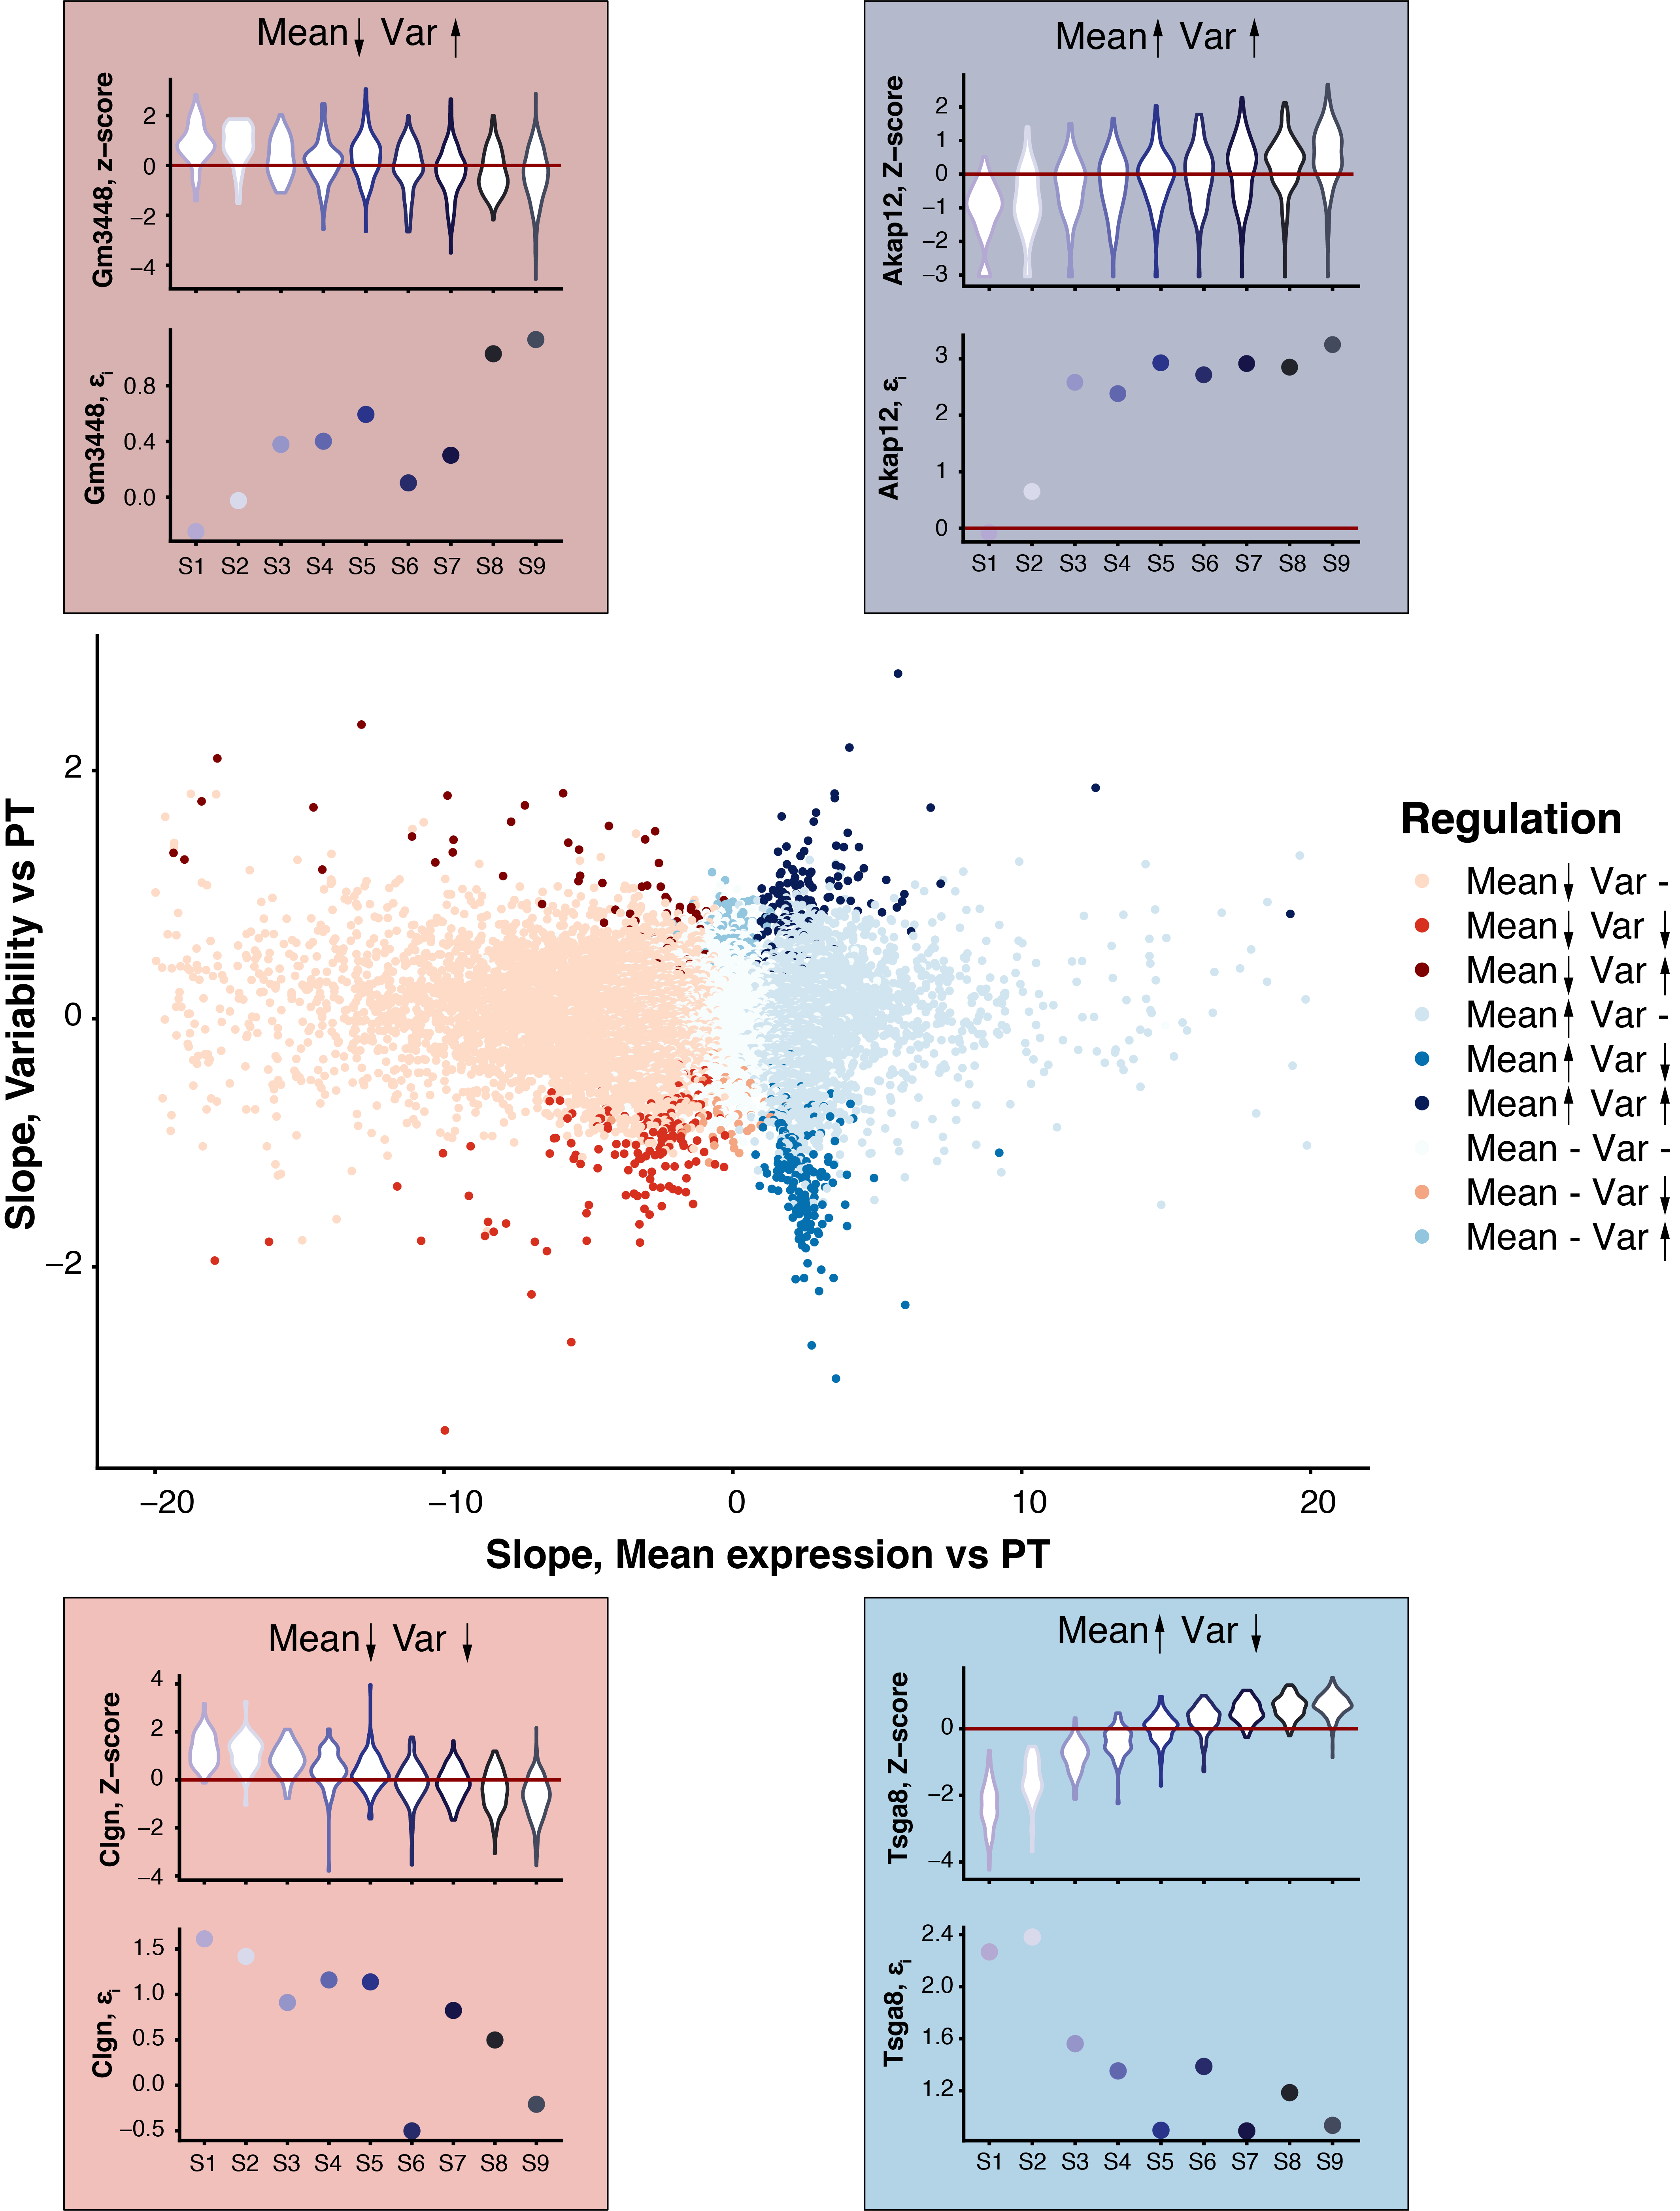
\includegraphics[width=\textwidth]{Fig_15.png}
\caption[Single-cell multi-omic approaches]{\textbf{Single-cell multi-omic approaches.}\\
Single-cell DNA and RNA-Seq either directly separates RNA and DNA or pre-amplifies both prior to separation. 
Measuring RNA and protein abundance from individual cells is done after physical separation followed by either oligonucleotide tagging of proteins or isotope tagging of RNA molecules. 
For methylome and transcriptome sequencing, DNA and RNA are separated prior to RNA sequencing and bisulfite conversion.}
\label{fig0:multiomics}
\end{figure}

Similarly, \gls{scMT-Seq} initially separates genomic DNA from mRNA. The scBS-Seq protocol is applied to isolated gDNA and is used to identify methylated CpG positions while mRNA was amplified via the SmartSeq2 protocol \citep{Angermueller2016a}. 
The scM\&{}T-Seq method has been extended to detect accessible chromatin regions in parallel to capturing methylated CpG sites and whole-transcriptome information. 
Prior to bisulfite conversion of gDNA, GpC sites are methylated by MTase in nucleosome sparse regions \textbf{(Fig.~\ref{fig0:multiomics})} \citep{Pott2017, Clark2018}.\\
 
Attempts have been made to capture $\sim$96 mRNAs in combination with proteins within individual cells. 
After cell lysis, samples are split to process mRNA and protein separately. 
mRNA is reverse transcribed and pre-amplified prior to \gls{qPCR} while oligonucleotide tagged antibodies bind to proteins. 
The free 3’-ends are complementary and can be extended by polymerisation to create a DNA reporter molecule. Similar to mRNAs, these molecules are detected using qPCR \citep{Darmanis2016}. 
This method has been scaled up by integration of droplet digital PCR \citep{Albayrak2016}. 
Alternatively, proximity ligation assay for RNA allows isotope tagging of RNA molecules, which are detected in parallel to proteins via mass cytometry \textbf{(Fig.~\ref{fig0:multiomics})} \citep{Frei2016}.

\subsection{Imaging approaches}

Similar to single-cell sequencing, RNA or protein imaging approaches quantify noise in biological systems \citep{Harton2017a}. 
Initial studies that addressed the extent of biological noise in bacterial populations used the expression of fluorescent proteins controlled by promoters of interest (reporter assays) to quantify expression noise \citep{Elowitz2002, Blake2003}. 
Later on, \gls{smFISH} was developed to capture variation in mRNA abundance across multiple cells \citep{Fang2013a, Lyubimova2013, Sanchez2013} and in whole organs \citep{Yang2014b}. 
Furthermore, the combination of fluorescently labelled proteins and smFISH allows the detection of co-variation between protein and mRNA levels within individual cells \citep{Taniguchi2011}. 
High-throughput automated smFISH of target RNAs in thousands of wells \citep{Battich2013} identified nuclear retention of RNAs as a mechanism to reduce cytoplasmic transcript variability \citep{Battich2015a}. 
Moreover, computerised image analysis and supervised machine learning extracts hundreds of cellular features from microscopy images and can therefore dissect variation of biological processes such as virus infection \citep{Snijder2009}.\\

The development of super-resolution microscopy allows detection of fluorophores that are spaced less than 100nm apart \citep{Sydor2015}. 
By combining \gls{STORM} and combinatorial labelling of RNA inside the cell, multiple transcripts from different genes can be visualised \citep{Lubeck2012}. 
This approach has been advanced to measure hundreds to thousands of RNA species per cell. 
\Gls{MERFISH} hybridises encoding probes to target RNAs prior to $N$ rounds of combinatorial labelling using fluorescently labelled read-out probes \textbf{(Fig.~\ref{fig0:MERFISH})}. 
MERFISH uses an encoding scheme that corrects for individual read-out errors based on a certain hamming distance between possible N-bit codes. 
Therefore, with 16 rounds of combinatorial labelling and a hamming distance of 4, 140 RNA species can be detected \citep{Chen2015}. A similar approach has been developed to profile spatial expression patterns in the mouse hippocampus (seqFISH) \citep{Shah2016}. 
By replacing the photobleaching step between consecutive rounds of combinatorial labelling with chemical cleavage and using multi-color imaging, the throughput of MERFISH can be increased \citep{Moffitt2016a}. 
Background fluorescence in tissue sections can be reduced by matrix-embedding of labelled RNA and cellular digestion \citep{Moffitt2016}.

\begin{figure}[!h]
\centering
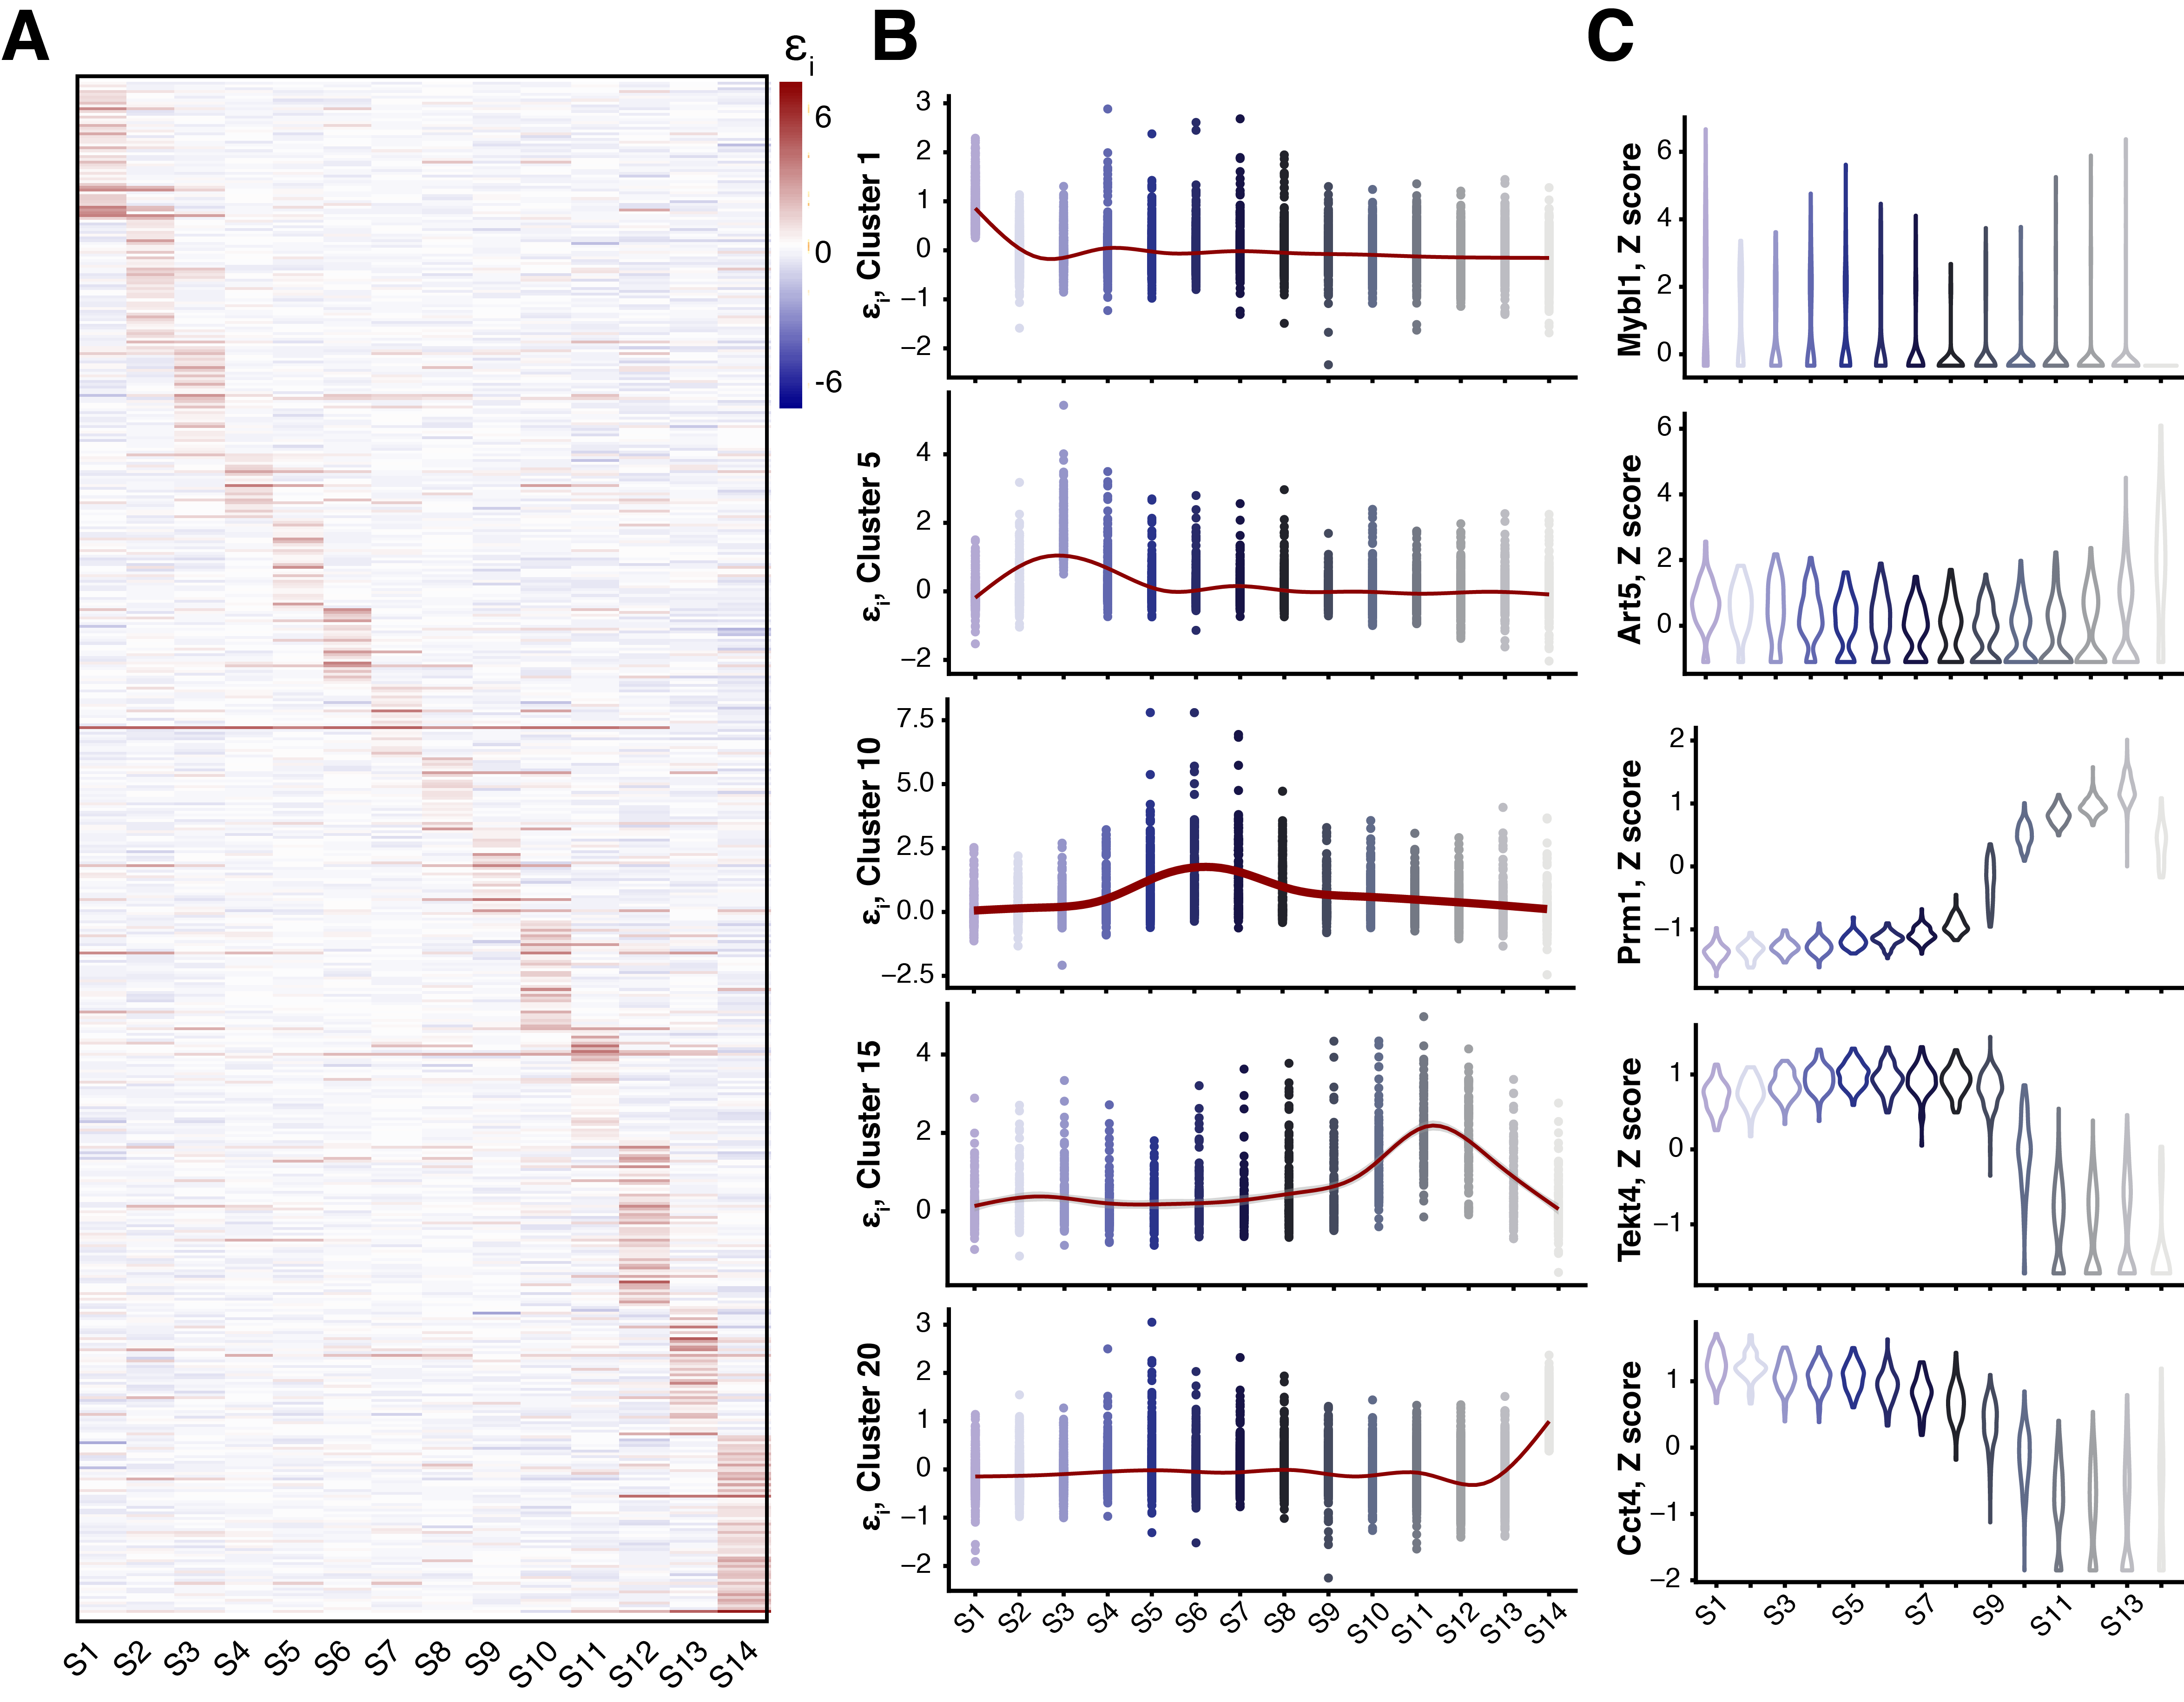
\includegraphics[width=\textwidth]{Fig_16.png}
\caption[MERFISH-type spatial transcriptomics]{\textbf{MERFISH-type spatial transcriptomics.}\\
Each transcript species is tagged with encoding probes that contain a sequence to recognise the RNA and multiple read-out sequences. 
During each hybridisation cycle, individual read-out probes hybridise with their specific sequences on the encoding probes. 
After multiple rounds of hybridisation and imaging, individual RNA transcripts can be decoded.}
\label{fig0:MERFISH}
\end{figure}

\subsection{Computational modelling and quantification}

Previous research focused on the derivation of mathematical frameworks to model expression dynamics in biological systems \citep{Tsimring2014}. 
In the simplest case, the central dogma of molecular biology states that mRNAs are synthesised from DNA at rate $k_m$ and proteins are translated from mRNAs at rate $k_p$. 
Furthermore, mRNAs are degraded at rate $\gamma_m$ and proteins at rate $\gamma_p$. 
In a noise-free system, this dogma leads to the following \textbf{deterministic}, first-order differential equation describing the number of mRNAs ($m$) and proteins ($p$) over time:

\begin{equation}
\frac{dm}{dt}=k_m-\gamma{}_mm,\quad \frac{dp}{dt}=k_pm-\gamma{}_pp
\end{equation}

\doublespacing
\noindent Steady-state transcript counts in this simple, two-stage system are defined as $\langle{}m\rangle{}=\frac{k_m}{\gamma_m}$  and protein abundance as $\langle{}p\rangle{}=\frac{k_mk_p}{\gamma_m\gamma_p }$. 
The variance for transcript and protein distributions are defined as: $\sigma^2=\langle{}m\rangle{}$ and $\sigma_p^2=\langle{}p\rangle{}\left[\frac{k_p}{\gamma_p+\gamma_m}+1\right]=\langle{}p\rangle{}\left[\frac{b}{1+\eta}+1\right]$, where $b=k_p/\gamma_m$  is the average number of proteins produced per transcript and $\eta=\gamma_p/\gamma_m$  \citep{Tsimring2014, Thattai2001}. 
mRNAs usually decay much faster than proteins. Therefore $\gamma_m\gg{}\gamma_p$ and $\sigma_p^2\cong\langle{}p\rangle{}\left[b+1\right]$ \citep{Thattai2001}. 
For this system, the mean translational burst size can be described as the Fano factor $\frac{\sigma_p^2}{\langle{}p\rangle}\cong{}b+1\approx{}b$ and burst frequency is captured by the inverse squared coefficient of variation $\frac{\langle{}p\rangle{}^2}{\sigma_p^2}\approx{}\frac{\langle{}p\rangle{}}{b}=\frac{k_m}{\gamma_p}=a$. The latter assumes that mRNAs are directly translated as soon as they are produced \citep{Friedman2006}.\\

\onehalfspacing
\noindent To account for stochasticity in this system, probabilistic expressions of the aforementioned equations have been described. 
The chemical master equation defines the time evolution of the probability of observing a system containing $m$ mRNAs and $p$ proteins at time point $t$:

\begin{align}
\frac{\partial{}P_{m,p}}{\partial{}t}&=k_m\left[P_{m-1,p}-P_{m,p}\right]+\gamma_m\left[(m+1)P_{m+1,p}-mP_{m,p}\right] \nonumber \\
&+k_pm\left[P_{m,p-1}-P_{m,p}\right]+\gamma_p\left[(p+1)P_{m,p+1}-pP_{m,p}\right]
\end{align}

\noindent The stationary probability distribution for this discrete representation of the master equation has the form of a negative-binomial distribution:

\begin{equation}
P_p=\frac{\Gamma(a+p)}{\Gamma(p+1)\Gamma(a)}\left(\frac{b}{1+b}\right)^p\left(1-\frac{b}{1+b}\right)^a
\end{equation}

\noindent where $a$ represents the burst frequency, $b$ the mean burst size and $\Gamma(n)$ the Gamma function \citep{Shahrezaei2008,Friedman2006,Tsimring2014}. 
Friedman \textit{et al.}, 2006 derived a stationary probability distribution from a continuous form of the chemical master equation \citep{Friedman2006}. 
This solution takes the form of a Gamma distribution:

\begin{equation}
P_p=\frac{1}{b^a\Gamma(a)}p^{a-1} e^{-p/b}
\end{equation}

\noindent This simple system has also been extended to incorporate the ON-OFF switching of promoters \citep{Jones2014, Shahrezaei2008}. 
Extensive modelling and quantification of mRNA and protein abundance in prokaryotic and eukaryotic cell populations confirmed this negative binomial (over-dispersed Poissonian) relationship between protein variance and abundance \citep{Ozbudak2002, Bar-Even2006}. 
The over-dispersion in protein abundance arises from biological noise ($\eta_{tot}$), which can be decomposed into intrinsic ($\eta_{int}$) and extrinsic ($\eta_{ext}$) contributions ($\eta_{tot}=\eta_{int}+\eta_{ext}$) \citep{Swain2002, Fu2016}. 
These components can be directly computed when using a two reporter system controlled by identical promoters \citep{Elowitz2002}. \\

Classic mathematical approaches to model transcriptional and translational dynamics use simplified assumptions for analytical tractability. 
Similar to the described translational bursting, transcriptional bursting as observed in eukaryotic cells \citep{Raj2006} leads to an over-dispersion in mRNA transcripts. 
Furthermore, while most models focus on single promoter dynamics, cases in which multiple promoters and competitor sites dilute TF binding have only recently been addressed \citep{Das2015a}. 
The assumption that translation from mRNA follows a first-order process was extended by using a hyperbolic Michaelis-Menten kinetic to model the translation process. 
This approach allows for continuous levels of ribosome occupancy on mRNAs \citep{VanDyken2017}. \\ 

While the models described above theoretically describe the expected distributions of proteins and mRNA across a population of cells, in practice, absolute measures (e.g.~transcript counts or fluorescence intensity) have to be used to quantify variation across a population of cells. 
In an early approach to model promoter kinetics from \gls{scRNA-Seq} data, Kim and Marioni, 2013 proposed a hierarchical Beta-Poisson model that relies on the switching dynamics of promoters between the "ON" and the "OFF" state ($k_{ON},k_{OFF}$) as well as the transcription rate $s$ and the decay rate $d$ \citep{Kim2013}. 
The model was formulated as follows:

\begin{align*}
X&|s,p\sim{}\text{Poisson}(sp)\\
p&|k_{ON},k_{OFF}\sim{}\text{Beta}(k_{ON},k_{OFF}),
\end{align*}

where $X$ is the transcript count per cell and $p$ a random effect dictated by promoter switching. 
Gene-specific inference was implemented as a Bayesian framework using Gamma distributions as priors for the hyper-parameters and Gibbs sampling to derive the posterior distributions of model parameters. 
The model indicates that RNAPII binding as well as histone modifications modulate burst size and burst frequency \citep{Kim2013}. \\

As an alternative, a variety of heterogeneity point estimates were computed to quantify biological noise. 
The variance $\sigma^2$, either calculated across all cells or across all expressing cells \citep{Shalek2014}, captures variability in RNA and protein abundance and scales linearly with mean expression $\mu$ \citep{Dey2015a}. 
The \gls{CV2} or the Fano factor are more widely used to measure heterogeneous RNA expression \citep{Brennecke2013, Jones2014} and protein abundance \citep{Newman2006}. 
Lowly expressed genes show higher levels of noise compared to highly expressed genes \citep{Brennecke2013}. 
Therefore, the CV$^2$ decreases with mean expression. 
To compare variability measures across different biological conditions where mean expression changes, regression approaches have been used to correct for the mean-variance relationship \citep{Kolodziejczyk2015cell, Fan2016}. 
Other approaches directly model biological variability as the excess in dispersion after removing technical noise \citep{Vallejos2015BASiCS}. 
Similar to the \gls{CV2} \citep{Brennecke2013} this over-dispersion measure decreases with increasing mean expression \citep{Vallejos2015BASiCS}. 
Moreover, heterogeneous expression can be captured by computing the Shannon entropy. Gene-specific entropy is defined as $H=-\sum_i{}p_i\log_2(p_i)$ where $p_i$ is the probability for a given gene being expressed in bin $i$. 
Binning across the expression counts can be done by choosing a fixed width \citep{Richard2016} or an adaptive width \citep{Stumpf2017}. 
Additionally, average pairwise distances between cells can capture increasing or decreasing heterogeneity in cell populations \citep{Mohammed2017}. \\ 

\newpage
%!TEX root = ../intro.tex
%******************************
%	 Other applications of scRNAseq
%*****************************

\section{General applications of scRNA-Seq in biology}

The following section outlines the broad spectrum of research fields that benefit from the development of scRNA-Seq technologies. Whole transcriptomic read-outs of individual cells allowed the in-depth characterisation of embryonic development, hematopoiesis, immune responses, allowed the detection of rare cell types and lead to new insights into disease progression including cancer development. 

\subsection{Atlas-type approaches}

Until recently, scRNA-Seq technologies were used to generate transcriptomes of less than a thousand cells to address specific questions in cellular systems such as cell-type heterogeneity, allele-specific expression or pseudo-temporal trajectories in gene expression \citep{Kolodziejczyk2015review}. With the development of scRNA-Seq technologies that massively increased the throughput of cell capture and data generation, cellular composition of whole tissues and organisms can be assayed. The largest of these so called "atlases" to date is the 10X Genomics\textsuperscript{\textregistered}{} brain dataset comprising 1.3 million cells from embryonic mice. I was generated using 133 libraries sequenced on 11 Illumina HiSeq\textsuperscript{\textregistered}{} 4000 flowcells \citep{Note2017}. This experiment has been performed to exemplify the applicability of the commercial 10X genomics platform to generate more than 10 billion transcriptomes of individual cells across the human body as envisioned by the Human Cell Atlas Consortium \citep{Regev2017}.\\

So far, examples of transcriptional atlases that comprise hundreds of thousands of cells are the mouse cell atlas, a thymus organogenesis atlas, an ageing lung atlas and the full characterisation of cell-types in \textit{C. elegans}. Similar to CytoSeq, Microwell-Seq was developed to capture more than 400,000 cells covering all mouse organ. This analysis reveals rare cell types, for example 2-cell-stage like mouse embryonic stem cells and allows the construction of a cross-tissue correlation network \cite{Han2018}. Similarly, the \emph{Tabula Muris} aimed at detecting all major cell type across 20 organs of the mouse. Here, the Tabular Muris Consortium decided to used droplet-based 3'-end scRNA-Seq and FACS-based full length transcript analysis to generate (i) a broad atlas and (ii) an in-depth characterisation of each tissue \citep{Quake2018}. Cao \emph{et al.}, 2017 generated more than 40,000 cells from the L2 stage \emph{C. elegans} using sci-RNA-Seq and identified nineteen distinct cell types and seven mixed cell types. Furthermore, this atlas allows the dissection of neuronal cell types that split across seven clusters \citep{Cao2017}. To study thymus development, Kernfeld \emph{et al.}, 2018 generated around 25,000 transcriptomes of individual cells from the embryonic thymus at E12.5, E13.5, E14.5, E15.5, E16.5, E17.5, E18.5, and P0. This experimental set-up resolves the temporal development of immune cell types such as T cells, myeolid cells, natural killer cells, innate lymphoid cells, and $\gamma{}\delta{}$ T cells as well as thymic epithelial cells \citep{Kernfeld2018}. Finally, to study the effect of ageing on a whole tissue, Angelidis \emph{et al.}, 2018 isolated 14,000 cells from lungs of young and old animals and found (i) and increase in transcriptional noise during ageing and (ii) altered transcriptional profiles of alveolar macrophages and type 2 pneumocytes \citep{Angelidis2018}.\\

The following paragraphs summarise scRNA-Seq applications which aimed at more targeted analysis of regulatory processes.

\subsection{Developmental biology}

For years, the development of new scRNA-Seq technologies and algorithms to perform data analysis uncovered driving factors in development and cell fate decisions \citep{Griffiths2018}. An early study during early mouse embryonic development identified that transcriptional differences between the two cells in the 2-cell stage embryo increase from the zygote to late 2-cell stage embryos. This is caused by an initial partitioning error where transcripts are unevenly distributed between the daughter cells and later on elevated by the onset of transcription coupled to transcriptional noise \citep{Piras2014, Shi2015a}. A reproducible distribution of transcripts in the first cell division was also detected by Biase \emph{et al.}, 2014 \cite{Biase2014}. These biases between cells at the 2-cell stage propagate to form transcription biases at the 4-cell stage to for the pluripotent inner cell mass or the extra-embryonic trophoectoderm \citep{Goolam2016, Shi2015a}. To obtain a more complete view on gastrulation in the mouse, Scialdone \emph{et al.} captured cells from the epiblast at E6.5 and mesodermal cells at E7.0, E7.5 and E7.75. The authors also sampled cells from \emph{Tal1} knock-out animals and showed that this transcription factor is the driving regulator for blood develeopment \citep{Scialdone2016}. \\

This year, large-scale scRNA-Seq studies profiled organogenesis in the mouse and zebrafish. Ibarra-Soria \emph{et al.} sampled more than 20,000 cells from E8.5 embryos following gastrulation and identified 20 major cell-types including different mesoderm lineages, neural progenitor cells, blood, gut and extra-embryonic cells. They further used this data to dissect gut formation and to find oscillating expression patterns during somitogenesis \citep{Ibarra-Soria2018}. Similarly, inDrop and Drop-Seq approaches were used to generate $\sim$7000 cells from \gls{Dmelanogaster} embryos at the onset of gastrulation todo{[rajewski reference]} or to generate more than 90,000 cells from the zebrafish embryo during the first day of development \citep{Wagner2018}.

In the last two years, experimental procedures were developed to track cells across multiple divisions termed "lineages". For this, the genome editing tool \gls{CRISPR}/\gls{Cas9} \citep{Jinek2012} was used to introduce so called "scares" at specific DNA sequences. In bacteria, the CRISPR/Cas system is used to degrade invasive DNA which involved a CRISPR RNA that recognizes the invading DNA and a Cas protein for degradation. For genome editing purposes, the \gls{CRISPR}/\gls{Cas9} uses guide RNAs to specific genomic sites and induces \gls{DSB}. Upon repair, insertions or deletion mutations are introduced that render a specific gene non-functional \citep{Zhang2014c}. The first approach to use the 	\gls{CRISPR}/\gls{Cas9} for scarring, \gls{GESTALT}, inserted an array of 10 \gls{CRISPR}/\gls{Cas9} with variable specificity into the genome of individual cells. Upon the expression of the Cas9 protein and the single-guide RNA, random scares are introduced into the genomic array. After days of growth genomic DNA was harvested and the array was sequenced to construct the relationship between individual cells \citep{McKenna2016}. This technology has been extended to a scRNA-Seq approach to capture the RNA together with the expressed \gls{CRISPR}/\gls{Cas9} array for cell-type detection and by a heat shock inducible system to start the scarring at later stages of development \citep{Raj2018}. Similar approaches uses multiplexed smFISH read outs to infer lineage relationship between individual cells \citep{Frieda2017} or tranposase-based insertion of a random 20mer sequence into the genome \citep{Wagner2018}.\\

One current challenge especially in the field of developmental biology is to obtain spatially-resolved whole-transcriptome read-outs of individual cells. The imaging technologies introduced above, MERFISH and SeqFISH, are capable of capturing single RNA molecules of thousands of genes across thousands of cells. Early approaches in the field of spatial transcriptomics employed spatial gene expression atlases to map isolated single cells back into the tissue of origin \citep{Achim2015a, Satija2015a}. A similar approach has recently been used to spatially locate cells isolated form the \gls{Dmelanogaster} embryo \todo{[rajewski reference]}. Moreover, Tomo-Seq was developed to sequence RNA extracted from slices of the zebrafish embryo. RNA was extracted from each slice into a tube and barcoded prior to sequencing. Matched histology and mathematical modelling was used to reconstruct the spatial expression patterns across the embryo \citep{Junker2014a}.

\subsection{Cell-type evolution} 

A smaller research field that uses scRNA-Seq approaches is evolutionary biology to understand the evolutionary origin of cell types. For this, non-model organisms such as \textit{Platynereis dumerilii} (annelid), \textit{Nematostella vectensis} (cniderian), \textit{Amphimedon queenslandica} (sponge), \textit{Mnemiopsis leidyi} (ctenophore) and \textit{Trichoplax adhaerens} (placozoan) are compared. All of these organisms (except annelids) are non-bilaterians and therefore evolutionary older than mouse and humans. As an example and part of an early project, we used the organism \textit{Platynereis dumerilii} to study diversification of cell-types in early bilaterian evolution. We detected cells from the apical neuroectoderm, the midgut, striated musculatrue, ciliated cells and non-apical blastopore cells. By assessing the transcriptional distance between these cell-types, we formulated a hypothesis of related cell-type families that originate from an ancesteral cell-type and are conserved during evolution \citep{Achim2018}.  \\

Seb\'e{}-Pedr\'o{}s \emph{et al.}, 2018 generated an single-cell genes expression atlas of adult and larval \textit{N. vectensis} using MARS-Seq. This dataset allowed the dissection of neuronal diversification and transcription factor regulatory programmes in this early sister group of bilaterians \citep{Sebe-Pedros2018}. The authors furthermore generated similar atlases of \textit{A. queenslandica}, \textit{M. leidyi} and \textit{T. adhaerens} and performed cross-species gene module analysis after cell-type identification. Co-regulation of cell-type-specific gene modules strongly diverged between the species except of few house keeping modules. Moreover, regulatory TF modules appear to be cell-type and species-specific \citep{Sebe-Pedros2018a}. These studies introduced scRNA-Seq as a powerful tool to study inter-species relationships of cell-types to dissect cell-type evolution. 

\subsection{Immunology}

The immune system has been extensively studied using scRNA-Seq to detect sub-cell-types, activation responses and to dissect the heterogenity of immune cells \citep{Proserpio2015, Satija2014}. White blood cells are broadly grouped into cells of the innate and adaptive immune system. Innate immune cells (dendritic cells, mast cells, macrophages, basophiles, \gls{NK} cells, neutrophils, eosinophil) are fast responders that represent the first line of defence in infections. The Adaptive immunity (B cells, CD4\plus{} and CD8\plus{} T cells) responds slower but installs an antigenic specificity and immune memory after infection \citep{Dranoff2004}. \\

\subsubsection{scRNA-Seq to study innate immunity}

Villani \emph{et al.}, 2017 used plate based scRNA-Seq to dissect the \gls{DC} and monocyte compartment of human \glspl{PBMC}. In general, DCs can be subdivided into CD11C\plus{} conventional DCs (CD141\plus{} and CD1C\plus{}) that activate CD4\plus{} and CD8\plus{} and interferon producing plasmacytoid DCs. Monocytes were classically subdivided into CD14\plus{} and CD16\plus{} cells. After analysing more than 2,400 DCs and monocytes, the authors expanded DCs to consist of 6 groups and detected conventional DC progenitor cells. Furthermore, they detected two new groups of uncharacterised monocytes \citep{Villani2017}. Shalek \emph{et al.}, 2014 used the C1 Fluidigm system to generate transcriptomes of more than 1700 primary mouse bone-marrow-derived DCs to study their activation response during \gls{LPS} stimulation. Within one hour of activation, early responding cells up-regulate \gls{Ifn}\textbeta{} and support the activation of surrounding cells via paracrine signalling. By isolating activated cells in individual chambers, the authors showed a decrease in the total number of activated cells after 4h stimulation with LPS. Furthermore, activated cells need autocrine stimulation to fully activate and IFN\textbeta{} secretion during the first hour of activation is the crucial trigger for full DC activation \citep{Shalek2014}. \\

Bj\"o{}rklund \emph{et al.}, 2016 performed targeted scRNA-Seq of Lin\textsuperscript{-}CD127\plus{} \glspl{ILC} and NK cells from tonsil tissue of adult humans using the SmartSeq2 protocol. They firstly identified the three major lineages of ILCs (ILC1, ILC2 and ILC3) and further assessed heterogeneity within the ILC3 population. Dissecting this rare cell-type allows a deeper understanding of immune regulation in humans \citep{Bjorklund2016}. 

\subsubsection{scRNA-Seq to study adaptive immunity}

An unbiased approach analysed $\sim$65,000 human \glspl{PBMC} and identified the major innate and adaptive immune cell-types. The authors further used droplet-based scRNA-Seq to study bone marrow mononuclear cells after hematopoietic stem cell transplant in order to treat \gls{AML}. The technology allowed the distinction between host and donor cells and the detection of residual AML cells in the host \citep{Zheng2017}. 

\subsection{Tissue function}

\todo{Mammary gland, liver}

\subsection{Cancer}

\todo{Avivs papers}
\newpage
%!TEX root = ../intro.tex
%******************************
%	 Bayesian approaches
%*****************************

\section{Bayesian approaches to model scRNAseq data}

As described above, expression counts in single-cell RNA-Seq data can be modelled as negative binomial distributed [ZINBABWE] while other approaches model these counts as log-normal distributed [BISCUIT, ZIFA]. This approach estimates cell and gene-specific parameters that can be used downstream for several tasks as normlization [Catas Nat Methods], clustering [ref], visualization [some latent space...] and imputation [MAGIC?], differential expression [e.g. MAST].   


\subsection{Scalability of Bayesian inference}

With the development of dropblet based approaches [Klein, Macosko] and multiplexed sequencing [Seqwell], scalability is important. 

Single-cell Variational Inference (scVI) 

scVI: transcriptomes of each cell are encoded through a non-linear transformation into a low-dimensional latent vector of normal random variables. latent representation is non-linearly transformed to generate a posterior distribution of model parameters based on a zer0-inflated negative binomial model. 

Zero-inflated negative binomial [Love 2014, Grun 2014, ZinBAWave]

The transcript count of gene $g$ in cell $n$ is modelled as zero-inflated negative binomial distributed:

\begin{align*}
x_{n,g} = 
 \left\lbrace
  \begin{aligned}
    &\textnormal{Poisson}(\phi_j\nu_j\mu_i\rho_{ij}), && i=1,...,q_0,j=1,...n;  \\ 
    &\textnormal{Poisson}(\nu_j\mu_i), && i=q_0+1,...,q,j=1,...,n,    	    
  \end{aligned}
\right.
\end{align*}

\subsection{Neural networks for modelling scRNA-Seq data}
 


\newpage
%!TEX root = ../intro.tex
%******************************
%	 Outline 
%*****************************


\section{Outline}

The overarching topic of this thesis is the quantification and interpretation of transcriptional noise as measured by scRNA-Seq. \textbf{Chapter 2} presents an initial experiment to study how  transcriptional noise effects the immune system. We see that transcriptional noise increases across multiple immune response genes during ageing which therefore could explain a disrupted immune response in older individuals. This finding has been published in following paper:

\begin{Abstract}
\hspace{-5mm} Celia P. Martinez-Jimenez$^\ast$, Nils  Eling$^\ast$, Hung-Chang Chen, Catalina A. Vallejos, Aleksandra Kolodziejczyk, Frances Connor, Lovorka Stojic, Tim F. Rayner, Michael J. T. Stubbington, Sarah A. Teichmann, Maike de la Roche, John C. Marioni, Duncan T. Odom. Ageing increases cell-to-cell transcriptional variability upon immune stimulation. \emph{Science}, 1436: 1433-1436, 2017, \\
($^\ast$ equal contributions) 
\end{Abstract}

Studying changes in variability between two conditions was restricted to genes that did not change in mean expression due to a strong confounding between variability and mean expression. In \textbf{Chapter 3}, I therefore extended the statistical framework from chapter 2 to correct for this confounding effect. This correction lead to (i) a stabilization of model parameters, (ii) expansion of the gene set that can be tested for changes in variability and (iii) a novel way of interpreting transcriptional dynamics. This project has been published as:

\begin{Abstract}
\hspace{-5mm} Nils Eling, Arianne C. Richard, Sylvia Richardson, John C. Marioni, Catalina A. Vallejos. \\
Robust expression variability testing reveals heterogeneous T cell responses. \emph{Cell Systems}, In press, 2018
\end{Abstract}

The extended model offers the unique opportunity to study changes in variability across multiple cell types even when mean expression changes. In \textbf{Chapter 4}, I apply the newly developed model to test changes in variability over pseudotime. For this, droplet-based scRNA-Seq data of mouse spermatogenesis was used to dissect the transcriptional dynamics during this developmental process. Parts of the study are available online as:

\begin{Abstract}
\hspace{-5mm} Christina Ernst$^\ast$, Nils Eling$^\ast$, Celia P. Martinez-Jimenez, John C. Marioni, Duncan T. Odom. Staged developmental mapping and X chromosome transcriptional dynamics during mouse spermatogenesis. \emph{bioRxiv}, 2018, ($^\ast$ equal contributions)
\end{Abstract}

Finally, I will discuss current challenges in modelling transcriptional noise from scRNA-Seq data and experimental strategies to modulate expression variability.

\newpage

\section{Other contributions}

Contributions to papers that are not discussed in this thesis are as follows:\\

\begin{Abstract}
Kaia Achim$^\ast$, Nils Eling$^\ast$, Hernando Martinez Vergara, Paola Yanina Bertucci, Jacob Musser, Pavel Vopalensky, Thibaut Brunet, Paul Collier, Vladimir Benes, John C. Marioni, Detlev Arendt. Whole-Body Single-Cell Sequencing Reveals Transcriptional Domains in the Annelid Larval Body. \emph{Molecular Biology and Evolution}, 35: 1047-1062, 2018, ($^\ast$ equal contributions)
\end{Abstract}

\begin{Abstract}
Christina Ernst, Jeremy Pike, Sarah J. Aitken, Hannah K. Long, Nils Eling, Lovorka Stojic, Michelle C. Ward, Frances Connor, Timothy F. Rayner, Margus Lukk, Robert J. Klose, Claudia Kutter, Duncan T Odom. Successful transmission and transcriptional deployment of a human chromosome via mouse male meiosis. \emph{eLife}, 5: e20235, 2016 
\end{Abstract}

%!TEX root = ../main.tex
%******************************
%	 Chapter 1 
%*****************************

\chapter{Ageing increases transcriptional noise in CD4$^+$ T cell activation}

\graphicspath{{"../../Dropbox (Cambridge  University)/Figures_for_thesis/Chapter1/"}}

\vfill

\begin{Abstract}
Ageing is characterised by progressive loss of physiological and cellular functions, but the molecular basis of this decline remains largely unexplored. Here, we explored how ageing impacts transcriptional dynamics using single-cell RNA-sequencing of over a thousand unstimulated and stimulated naive and effector memory CD4$^+$ T cells from young and old mice. Furthermore, we sampled cells from two divergent strains of mice to assess the evolutionary conservation of the molecular ageing signature. In young animals, immunological activation drives a transcriptomic switch from variable to tightly regulated gene expression, characterised by a strong up-regulation of a core activation program, coupled with a decrease in cell-to-cell variability. The up-regulation of a set of immune response genes is conserved between the two mouse strains as is the decrease in expression variability upon immune activation. Ageing significantly perturbed the activation of the core immune response program by increasing expression heterogeneity across different populations of CD4$^+$ T cells. This discovery adds transcriptional noise as an unexplored hallmark of ageing to the list of known phenotypic changes.
\end{Abstract}

\vfill

\newpage

\begin{Comment}
\textbf{Declaration} This work was a joint effort of the Marioni, Odom, de la Roche and Teichmann labs. Celia P. Martinez-Jimenez, Duncan T. Odom, John C. Marioni and Sarah Teichmann designed the study. Celia P. Martinez-Jimenez and Aleksandra A. Kolodziejczyk performed preliminary experiments. Celia P. Martinez-Jimenez performed all single-cell RNA sequencing experiments displayed in this chapter. Hung-Chang Chen and Maike de la Roche provided extensive support during the revision process. Hung-Chang Chen performed FACS experiments during the revision process. Lovorka Stojic and Frances Connor provided experimental support. Timothy F. Rayner provided technical support. Michael J. T. Stubbington performed the T cell receptor and clone analysis. Catalina A. Vallejos helped with the statistical analysis by providing additional explanations of the BASiCS model. Celia P. Martinez-Jimenez and I interpreted results. Celia P. Martinez-Jimenez, Duncan T. Odom, John C. Marioni and I wrote the manuscript. Duncan T. Odom and John C. Marioni supervised the study. I performed computational analysis of all data displayed in this chapter and generated all figures with the exception of the FACS analysis (Fig. \ref{fig1:FACS} and Fig. \ref{fig1:EM_Naive_CD4}A-C). The paper has been published as:\\

Celia P. Martinez-Jimenez$^\ast$, Nils  Eling$^\ast$, Hung-Chang Chen, Catalina A. Vallejos, Aleksandra Kolodziejczyk, Frances Connor, Lovorka Stojic, Tim F. Rayner, Michael J. T. Stubbington, Sarah A. Teichmann, Maike de la Roche, John C. Marioni, Duncan T. Odom. Ageing increases cell-to-cell transcriptional variability upon immune stimulation. \emph{Science}, 1436: 1433-1436, 2017, ($^\ast$ equal contributions)
\end{Comment}

\begin{figure}[hb]
\centering    
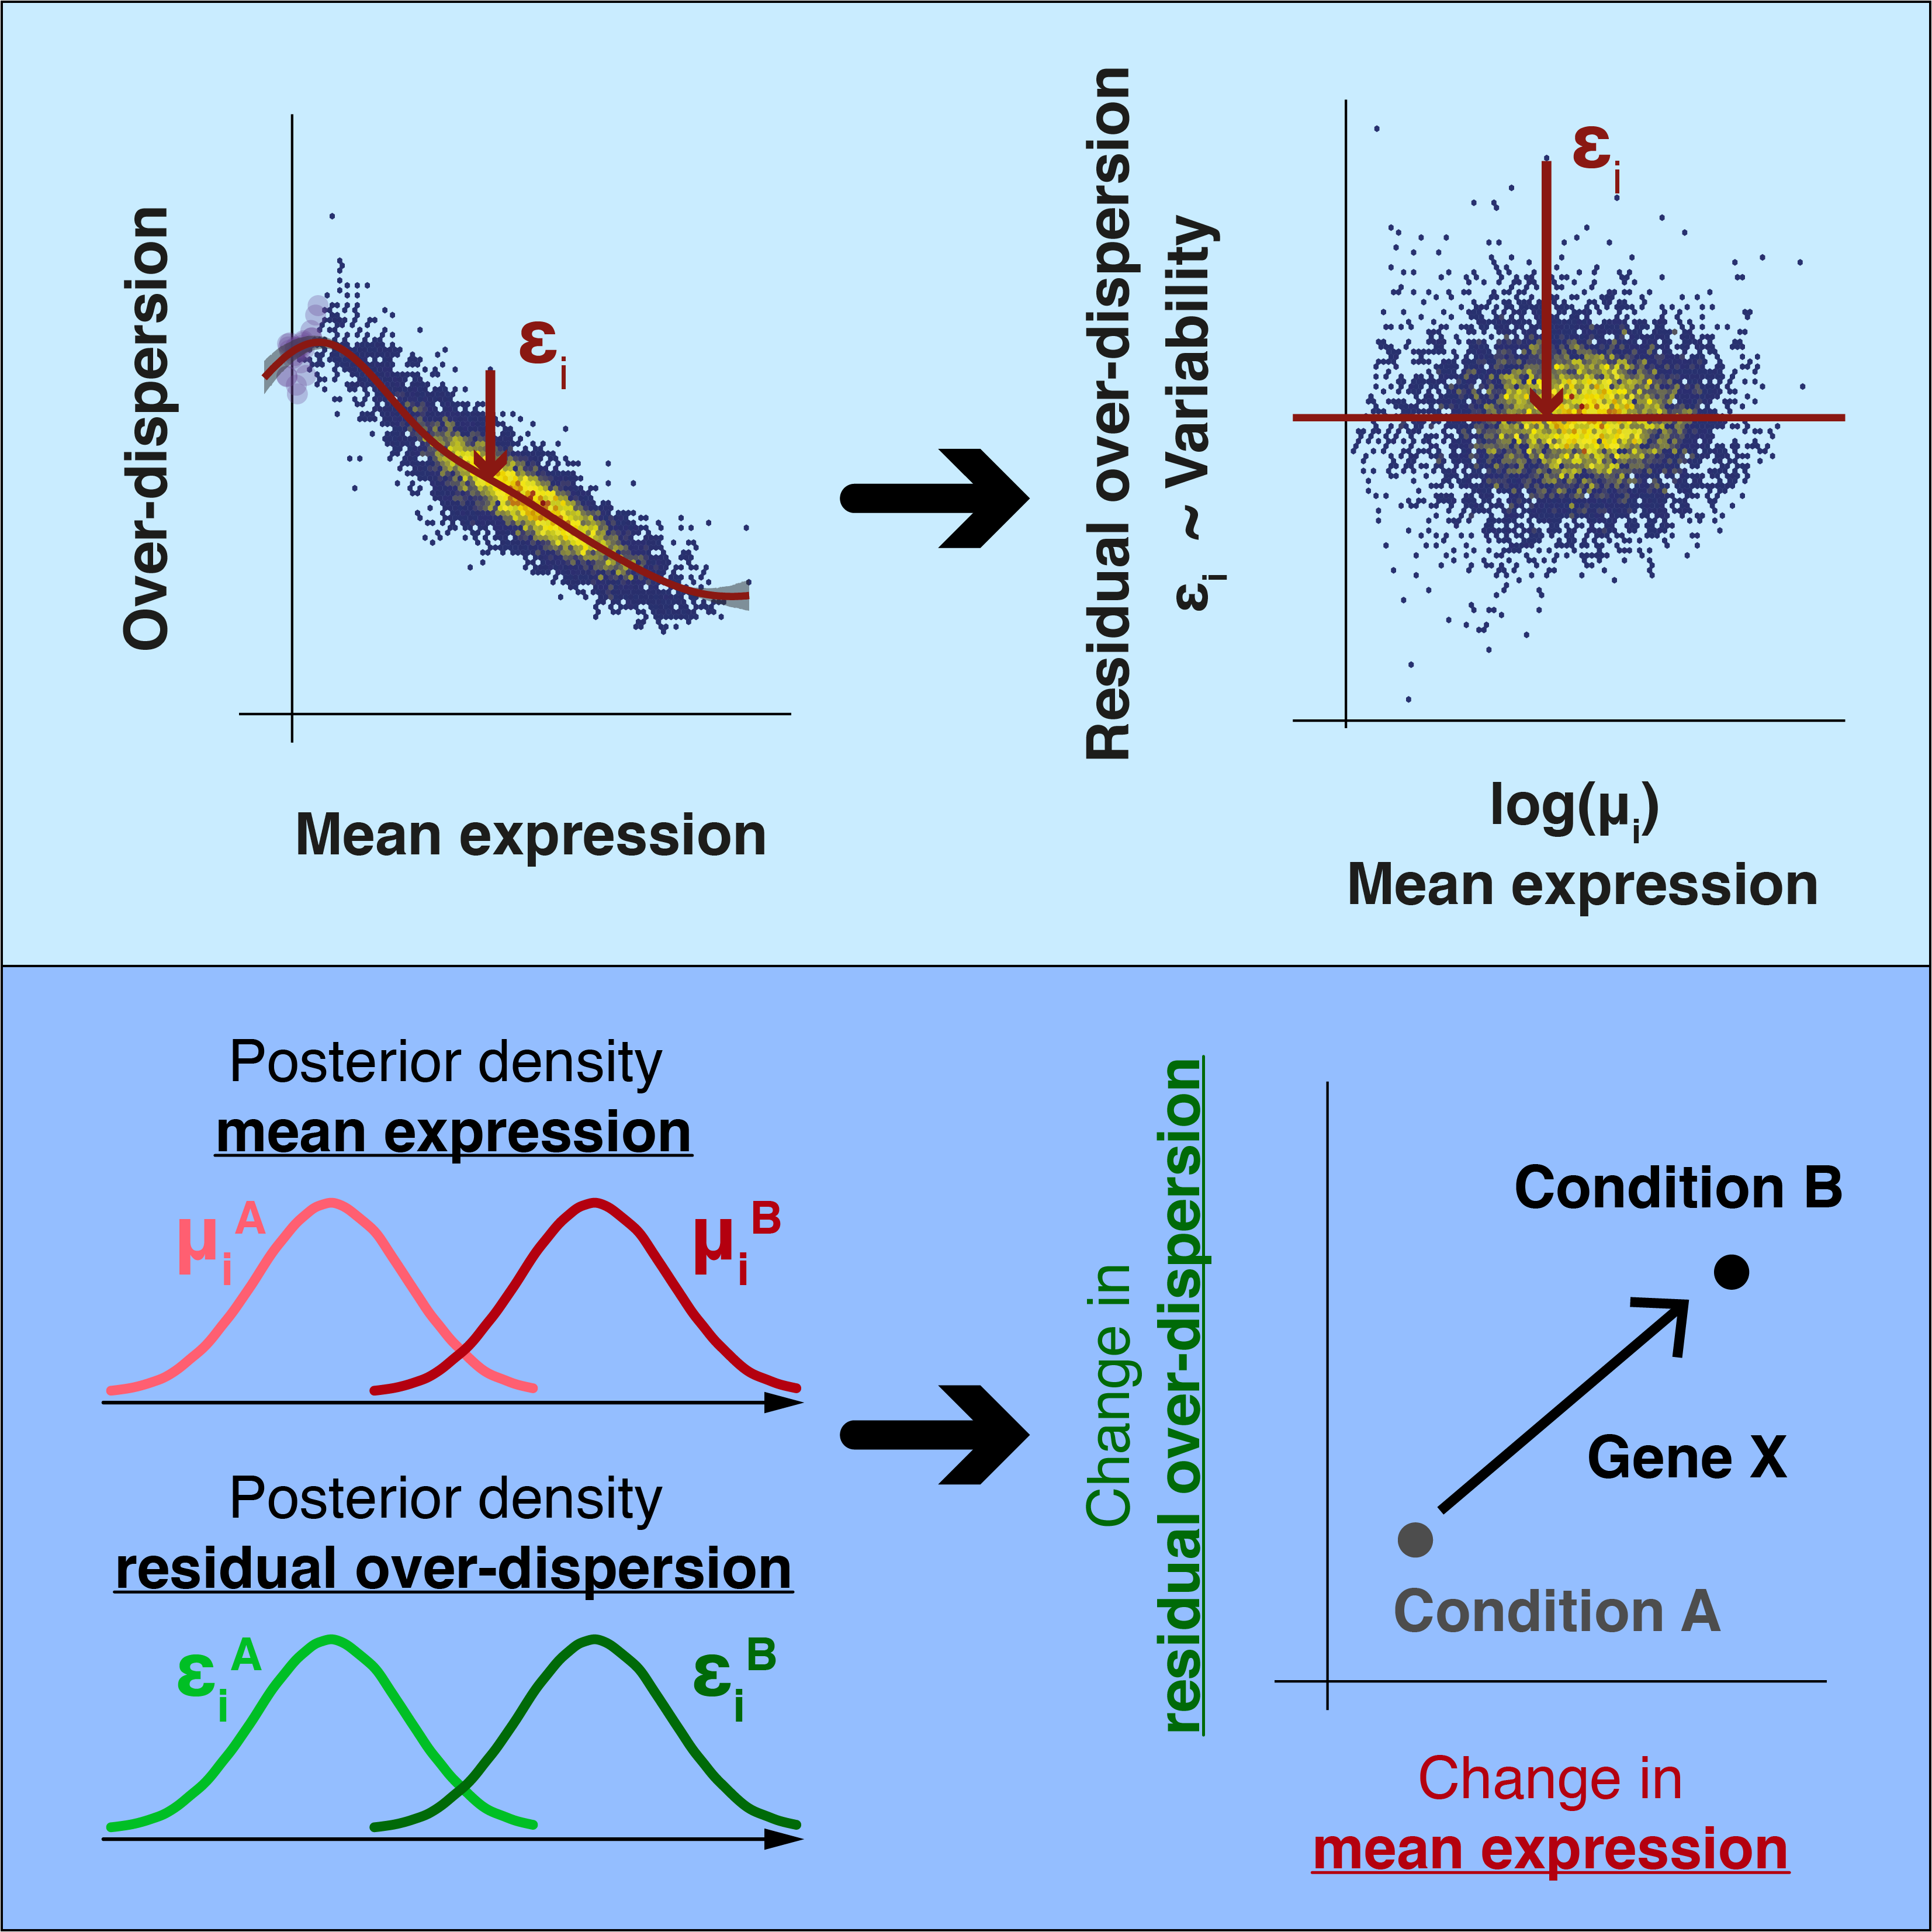
\includegraphics[width=0.8\textwidth]{GraphicalAbstract.png}
\end{figure}

\newpage

% Include different main sections of the first chapter
%!TEX root = ../chapter1.tex
%******************************
%	 Introduction 
%*****************************

\section{Introduction}

Ageing is characterized by the progressive decline of physiological and cellular functions \citep{Lopez-Otin2013, Booth2016}. Nine hallmarks of ageing have been described to determine the ageing phenotype: genomic instability, telomere attrition, epigenetic alterations, loss of proteostasis, de-regulated nutrient sensing, mitochondrial dysfunction, cellular senescence, stem cell exhaustion, and altered intercellular communication \citep{Lopez-Otin2013}. Ageing can have a complex and tissue-specific impact on gene expression levels \citep{Zahn2007}, as seen by microarray expression analyses of collections of mouse CD4$^+$ and CD8$^+$ T cells \citep{Mirza2011}, rat hepatocytes \citep{Tollet-Egnell2000}, mouse and human brain \citep{Lu2004, Lee2000}, human muscle \citep{Welle2003, Zahn2006}, human kidney \citep{Rodwell2004}, human retina \citep{Yoshida2002}, and different species of Drosophila and Caenorhabditis \citep{Mccarroll2004}. For instance, ageing affects distinct functional pathways, even in closely related CD4$^+$ and CD8$^+$ T cells \citep{Mirza2011}. \\

Approaches that analyse the expression of sets of genes on a single-cell basis have more recently suggested that ageing may also alter the cell-to-cell variability of gene expression. Transcriptional noise, RNA processing aberrations, impaired DNA repair, and chromosomal instability can be caused by epigenetic changes occurring in DNA methylation, histone modifications and chromatin remodelling \citep{Lopez-Otin2013}. DNA methylation slightly decreases globally but increases in common disease-related genes over the lifespan of humans \citep{Talens2012}. In mice, around 35\% of assayed genes showed either increased or decreased DNA methylation over ageing displaying strong tissue-specificity of the process \citep{Maegawa2010}. Similarly, ageing introduces changes of histone modifications such as the increase of H4K16ac, H4K20me3 and H3K4me3, as well as the decrease of H3K9me or H3K27me3 \citep{Han2012, Fraga2007}. One well studied system that controls cellular function is the \emph{Sir2} histone deacetlyase which is encoded by seven homologs in mammals \citep{Houtkooper2016}. The chromatin-associated protein SIRT6 in mice has been shown to protect genomic stability by promoting resistance to DNA damage. Loss of this protein induces ageing-realted phenotypes within 4 weeks of murine lifespan \cite{Mostoslavsky2006}.\\

While most studies focused on identifying age-associated gene expression profiles \citep{DeMagalhaes2009}, the role of transcriptional noise during ageing has only been sporadically assessed. Analysis of fifteen genes in terminally differentiated cardiomyocytes suggested that ageing can lead to increased cell-to-cell transcriptional variability \citep{Bahar2006}. In contrast, single-cell analysis of the transcription of six genes in four different hematopoietic stem cell types showed few cell-to-cell changes between old and young animals, leading to the suggestion that transcriptional instability may not be a universal attribute of ageing \citep{Warren2007}. Whether cell-to-cell gene expression variability increases during ageing on a genome-wide basis, particularly for dynamic activation programs, remains largely unexplored.\\

Single-cell RNA sequencing presents a powerful technology to quantify  transcriptional variability in thousands of genes across thousands of cells simultaneously. For example, Kowalczyk \textit{et al.} performed a high-resolution scRNA-seq analysis of hematopoietic stem cells in young and old mice. Here, cell cycle is the primary driver for cell-to-cell variability in gene expression, and ageing decreases the entry of long-term hematopoietic stem cells into G1 phase in a cell-type-specific manner \citep{Kowalczyk2015}.\\ 

To evaluate the impact of ageing on gene expression levels and cell-to-cell transcriptional variability, we selected CD4$^+$ T cells as model system. As explained in \textbf{Box 1}, transcriptional noise is defined as cell-to-cell variability in expression within a homogeneous population of cells. Naive CD4$^+$ T cells are readily isolated as single, phenotypically homogeneous cells when purified from young and aged spleens and can be easily stimulated into a physiologically-relevant activated transcriptional state in vitro. Furthermore, they are maintained in a quiescent state, but have the ability to respond to antigen stimulation with proliferation and effector differentiation, which is essential for life-long maintenance of adaptive immune function against infection and cancer \citep{Swain2012, Kim2014a}. With this, they sit at the root of adaptive immunity and disruption of their transcriptional programme can lead to severe phenotypes during ageing. \\

Previously, comparing gene expression levels in matched tissues from different mammalian species was used as a tool for revealing conserved cell-type-specific regulatory programs \citep{Sudmant2015, Finseth2014, Brawand2011, Flajnik2009}. For instance, a conserved set of response genes has been identified by comparison of bulk gene expression between human and mouse CD4$^+$ T cells after immune activation \citep{Shay2013}. So far, it is not known whether conservation of gene expression levels is also reflected in cell-to-cell variability.\\

Here, we dissect the activation dynamics of naive CD4$^+$ T cells at the single cell level during ageing in two sub-species of mice. With this, we can assay transcriptional dynamics during immune response and how ageing possibly perturbs this system. By comparing our findings across divergent strains of mice, we can assess the evolutionary conservation of the immune response and ageing phenotype. Furthermore, we isolated pure naive and effector memory CD4$^+$ T cells to profile age-related changes in different CD4$^+$ T cell subsets.

\newpage
%!TEX root = ../chapter1.tex
%******************************
%	 Results 
%*****************************

\section{scRNAseq of murine CD4$^+$ T cells}
\subsection*{Single-cell RNA sequencing of CD4$^+$ T cells during activation, ageing and across two mouse species}

To assess the conservation of immune activation programmes, we isolated CD4$^+$ T cells from healthy individuals of two inbred mouse sub-species separated by 1 million years of divergence: the reference C57BL/6J, Mus musculus domesticus (B6); CAST/EiJ, Mus musculus castaneus (CAST)). We characterized their gene expression programmes by single-cell RNA-sequencing (scRNAseq) during ageing in young (~3 months) and old (~21 months) individuals of each strain (Fig. \ref{}). These two sub-species have similar lifespans (23, 24), and CAST mice showed the hallmarks of normal organismal aging observed in B6 mice (25). All mice were healthy at the time of experiments. 

\subsubsection*{Unstimualted CD4$^+$ T cells}

\subsubsection{Naive and effector memory CD4$^+$ T cells}

\subsubsection*{Computational quality control and filtering}

from spleens and characterized their gene expression programs by single-cell RNA-sequencing (scRNA-seq) during aging in young (~3 months) and old (~21 months) individuals of each strain (Fig. 1A, Material and Methods).  

Purified naive CD4+ T cells were either loaded directly into the Fluidigm C1 system, or were loaded three hours after stimulation in vitro with plate-bound anti-CD3$\epsilon$/anti-CD28 antibodies (see Material and Methods). Hereafter, for simplification and clarity, purified unstimulated naive CD4+ T cells will be named naive, and stimulated cells will be named activated. For each species/condition, scRNA-seq experiments were performed using cells isolated from two individual mice. We visually inspected the vast majority of cell-capture sites in each C1 small-integrated fluidic circuit (IFCs, 5-10$\mu$m) using 40x magnification lensing to ensure precise capture of single cells (Fig. S1A and S1B and Material and Methods). We removed low-quality C1 captured cells by evaluating (i) the sequencing depth, (ii) the number of genes detected, (iii) the proportion of sequencing reads mapping to exons and ERCC controls, and (iv) the mitochondrial fraction of reads (Fig. S1C-F). The resulting data showed minimal batch effects (Fig. S1G). Using RNA-sequencing to identify cell-specific marker genes, we removed residual B-cells, CD8+ T cells, and (in activating conditions) non-activated T cells from our analysis (Fig. S1H and S1I, Material and Methods). \\

In contrast to haematopoeitic cells (15), even when activated, virtually all CD4+ T cells are in G1 phase of cell cycle as expected (Fig. S2A). Aged CD4+ T cells showed no clonal expansions (Fig. S2B) or difference in cell size (Fig. S2C) that could impact analysis of gene expression variability (26). Using flow cytometry analysis, we confirmed that 96.4\% of the isolated CD4+ T cells were naive in young B6 (Fig. S2D). Naive CD4+ T cells formed a single, high-purity population in young animals. Old animals had a small population of CD4+ T cells with slightly elevated CD44 levels, reduced CD62L expression, and attenuated activation dynamics (Fig. S2E-G); their removal did not impact our results (Material and Methods) (see below). Upon T cell receptor (TCR) activation in the presence of particular cytokines, naive CD4+ T cells can differentiate into several lineages of functionally different T helper cells (mainly Th1, Th2, Th17, Treg, Tfh) (16, 27). In our data we do not detect any early differentiation in naive and activated CD4+ T cell subsets. In accordance with the literature we found Gata3 but not Th2 cytokines expressed in the majority of cells  (28). Interestingly, the Th1-related genes Tbx21 and Ifng were up-regulated, in an uncoordinated manner, in a small population of activated CD4+ T cells of old animals. This is consistent with a known Th1 bias in CD4+ T cell responses in old mice (29) and humans (30) (Fig. S2H). Furthermore, we did not detect any difference in TCR components/signaling and importantly detected no signs of T cell exhaustion (31), especially in cells isolated from old animals (Fig. S2I). We also ruled out species-specific differences in commitment towards T helper cell lineages (Fig. S2J). \\

After the above analyses and the experimental validation (Material and Methods), a total of 1514 high-quality CD4+ T cell transcriptomes were analyzed across all conditions and species.


\newpage
%!TEX root = ../chapter1.tex
%******************************
%	 Discussion 
%*****************************

\section{Discussion}

How cell-type-specific gene expression programs change during organismal lifespan has long been debated \citep{Bahar2006, Warren2007} but until the beginning of this project, few studies in mammals have quantified the cell-to-cell transcriptome-wide differences that accumulate during ageing \citep{Kowalczyk2015}. Here, we systematically explored the effect of ageing on the dynamic activation program of primary naive CD4\plus{} T cells. We analysed two sub-species of mice, which represents a powerful strategy to identify evolutionarily conserved gene expression programmes \citep{Shay2013}. In contrast to humans, mice were housed in specific pathogen-free facilities that reduces transcriptional changes due to pathogen-induced immune activation \citep{Beura2016}. In this chapter, we therefore profiled the intrinsic effect of ageing on transcriptional regulation in CD4\plus{} T cells.\\

By activating naive CD4\plus{} T cells and quantifying the transcriptional responses of hundreds of single-cells using scRNA-Seq, we confirmed that translation processes and immune response genes are rapidly up-regulated \citep{Asmal2003, Neme2016, Turner2014, Glass2010, Gerondakis2010, Croft2009}. More interestingly, we discovered that transcriptional variability is reduced across thousands of transcripts that otherwise remain stable in mean expression levels. This indicates that immune activation rapidly reduces transcriptional heterogeneity across the population of CD4\plus{} T cells to up-regulate a specific response programme similarly in each individual cell. A similar programme has been identified in iPSC reprogramming where an early phase is characterised by probabilistic events while, later, the transcription of \textit{Sox2} induces a  more deterministic phase \citep{Buganim2012}. Previous studies assayed heterogeneity in immune responses by profiling individual cytokines such as interleukin 2 and interferon \textbeta{} in immune cells. Early responding cells support the activation of surrounding cells by paracrine signalling \citep{Fuhrmann2016, Shalek2014}. In contrast, by profiling thousands of genes, our approach identifies the global collapse of variability as a key event in immune activation.\\

Comparison of gene expression levels across species have been used as a means to identify transcription under strong selection in tissues \citep{Sudmant2015, Brawand2011, Romero2012, Barbosa-Morais2012, Perry2012}, including bulk CD4\plus{} T cells from young mice and humans during immune stimulation \citep{Shay2013}. By profiling two sub-species of mice, we identified a common set of activation genes, including well-characterised immune response genes such as \textit{Il2ra}, that are similarly up-regulated across the two species. Furthermore, using scRNA-Seq allowed us to determine the number of cells that express a certain gene. With this, we newly revealed that immune stimulation results in the vast majority of cells within each species up-regulating the set of evolutionarily conserved genes. In contrast, we discovered that genes whose mean expression was up-regulated in a species-specific manner were often activated in only a small fraction of cells, suggesting weaker selection. Indeed, species-specific up-regulated genes showed no functional enrichment. This discovery suggests a novel defining feature of functional target genes: coherent transcriptional up-regulation across a population of cells. \\

Many attempts have been made to identify transcriptional signatures associated with ageing \citep{DeMagalhaes2009, Magalhaes2009, Chen2013, Kowalczyk2015}. On a genome-wide basis, we observed that ageing has minimal effects on mean expression levels in unstimulated and stimulated CD4\plus{} T cells. However, in the core set of activated genes, in both species and in distinct CD\plus{} T cell subsets, we found a markedly more heterogeneous transcriptional response to stimulation in older mice. This increased heterogeneity was driven by ageing associated differences in the (reduced) fraction of cells across the population that express these response genes. Instead of detecting structured heterogeneity, characterised by some cells not responding to the stimulus, we observed that all cells from old animals responded, but in contrast to young cells, failed to homogeneously up-regulate the response programme. \\

High numbers of CD4\plus{} T cells are needed to combat infection and cancer. The discovery that CD4\plus{} T cells from aged mice are unable to up-regulate a core activation program robustly may in part explain the decrease of immune function observed in aged mammals \citep{Goronzy2013, Nikolich-Zugich2018}. More generally, in the context of the current understanding of transcriptional dysregulation and chromatin destabilization during ageing \citep{Booth2016}, increased cell-to-cell transcriptional variability is a major, and largely unexplored, intrinsic factor.\\

Following the publication of this study, several mechanisms for the increase in transcriptional variability during ageing have been proposed. In one study, the increase in transcriptional variability during ageing was confirmed in human pancreatic \textbeta{}-cells. A possible mechanism for this increase in variability is so called "fate drift" of \textbeta{}-cells to resemble \textalpha{}-cells. During ageing, \textbeta{}-cells that are defined by their expression of the hormone \emph{insulin} increase expression of the hormone \emph{glucagon}, the characteristic hormone of \textalpha{}-cells. This atypical hormone expression can result in increased transcriptional noise during ageing in the pancreas \citep{Enge2017}. Another study by Desch\^{e}nes and Chabot, 2017 proposed that the stochastic shortening of telomeres during ageing introduces variation in a process termed Telomere Position-Effect On Long Distance (TPE-OLD). 	TPE-OLD regulates the expression of genes 10 Mb into the chromosome and its variation can lead increased transcriptional heterogeneity during ageing \cite{Deschenes2017}. Further, Cheung \emph{et al.}, 2018 profiled a variety of epigenetic marks in different subsets peripheral blood mononuclear cells (PBMCs) in young (< 25 years) and old (> 65 years) humans at single-cell resolution \citep{Cheung2018}. Analysis of 40 chromatin marks in 20 cell types revealed a separation between young and old individuals and an enrichment in most chromatin marks during ageing. Furthermore, they found an increase in cell-to-cell variability for the majority of chromatin marks in aged individuals. The authors proposed a possible role for polycomb-repressive complexes (PRC) in increasing epigenetic variation and showed that PRC-mediated H3K27me3 deposition explains the increase in transcriptional variability that we reported in this chapter \citep{Cheung2018}.\\

While an increase in transcriptional noise has been shown to be associated with tissue ageing in pancreas and the immune system, a more complete view of whole-organism tissue ageing is missing. One study that begins to address this profiled changes in transcriptional noise in multiple cell types in young and old mice \citep{Angelidis2018}. Not only did they confirm the increase in transcriptional noise during ageing in CD4\plus{} T cells but also observed this shift in a variety of cells types associated to the lung (e.g. NK cells, macrophages, dendritic cells, endothelial cells, smooth muscle cells and neutrophils) \citep{Angelidis2018}. This analysis validates increased transcriptional noise as a major hallmark of ageing. \\

The major drawback in this chapter was the inability to profile all immune response genes for changes in variability due to the dependency of the over-dispersion parameter on the mean expression parameters (see \textbf{Section \ref{sec0:BASiCS}}). The simple approach to only profile genes with stable mean expression levels during immune activation excluded all immune-associated genes from analysis. These are generally the genes that define T cell phenotypes and functionality. In the next chapter, I will therefore describe an extension of the BASiCS framework to include genes that display changes in mean expression by regressing out this mean-variability dependency.







%!TEX root = ../main.tex
%******************************
%	 Chapter 2
%*****************************

\chapter{Addressing the mean-variability dependency in scRNA-Seq data}  

\graphicspath{{"../../Dropbox (Cambridge  University)/Figures_for_thesis/Chapter2/"}}

\vfill

\begin{Abstract}
\hspace{-5mm} As shown above, cell-to-cell transcriptional variability in otherwise homogeneous cell populations plays an important role in immune activation and increases with age. Single-cell RNA sequencing can characterise this variability in a transcriptome-wide manner. However, the confounding between variability and mean expression estimates hinders meaningful comparison of expression variability between cell populations. To address this problem, we introduce a statistical approach that extends the BASiCS framework to derive a residual measure of variability that is not confounded by mean expression. This measure is used to test changes in variability in parallel to changes in mean expression on a gene-specific level. With this method, we assessed changes in variability for genes responding to CD4\plus{} T cell activation and detect a synchronisation of biosynthetic machinery components. Furthermore, cytokines such as Il2 that support the activation of surrounding cells by paracrine signalling are heterogeneously up-regulated upon immune activation. When profiling more subtle transcriptional changes during CD4\plus{} T cell differentiation, we detect opposing patterns of changes in variability between \textit{Tbx21} and \textit{Cxcr5}, which are markers for Th1 and Tfh cells, indicating a delayed commitment process throughout differentiation. Finally, we confirmed the applicability of the newly extended BASiCS model to droplet-based scRNA-Seq data which is necessary for the subsequent chapter.
\end{Abstract}

\vfill

\newpage

\begin{Comment}
\hspace{-3mm} \textbf{Declaration} I worked on this project in close collaboration with Catalina Vallejos, Arianne Richard, Sylvia Richardson and John Marioni. In this project, I extended an existing Bayesian framework (BASiCS) that was developed to model scRNA-Seq data. Besides calculating the underlying math and programming the model, I helped re-write the BASiCS R package, which is now published on \href{https://bioconductor.org/packages/release/bioc/html/BASiCS.html}{Bioconductor}. Catalina Vallejos co-supervised me and introduced me to principles of Bayesian statistics. Arianne Richard helped with the interpretation of biological data and helped writing the manuscript. Sylvia Richardson provided statistical help on a part of the project that is not presented here. John Marioni co-supervised me and suggested analysis to be performed. Catalina Vallejos, John Marioni and I designed the study. Catalina Vallejos, John Marioni and I wrote the manuscript. I kindly thank Dominic Gr\"un for providing the smFISH data matched to mESC scRNA-Seq data. The study has been published as:\\

Nils Eling, Arianne C. Richard, Sylvia Richardson, John C. Marioni, Catalina A. Vallejos. Robust expression variability testing reveals heterogeneous T cell responses. \emph{Cell Systems}, In press, 2018 
\end{Comment}

\begin{figure}[hb]
\centering    
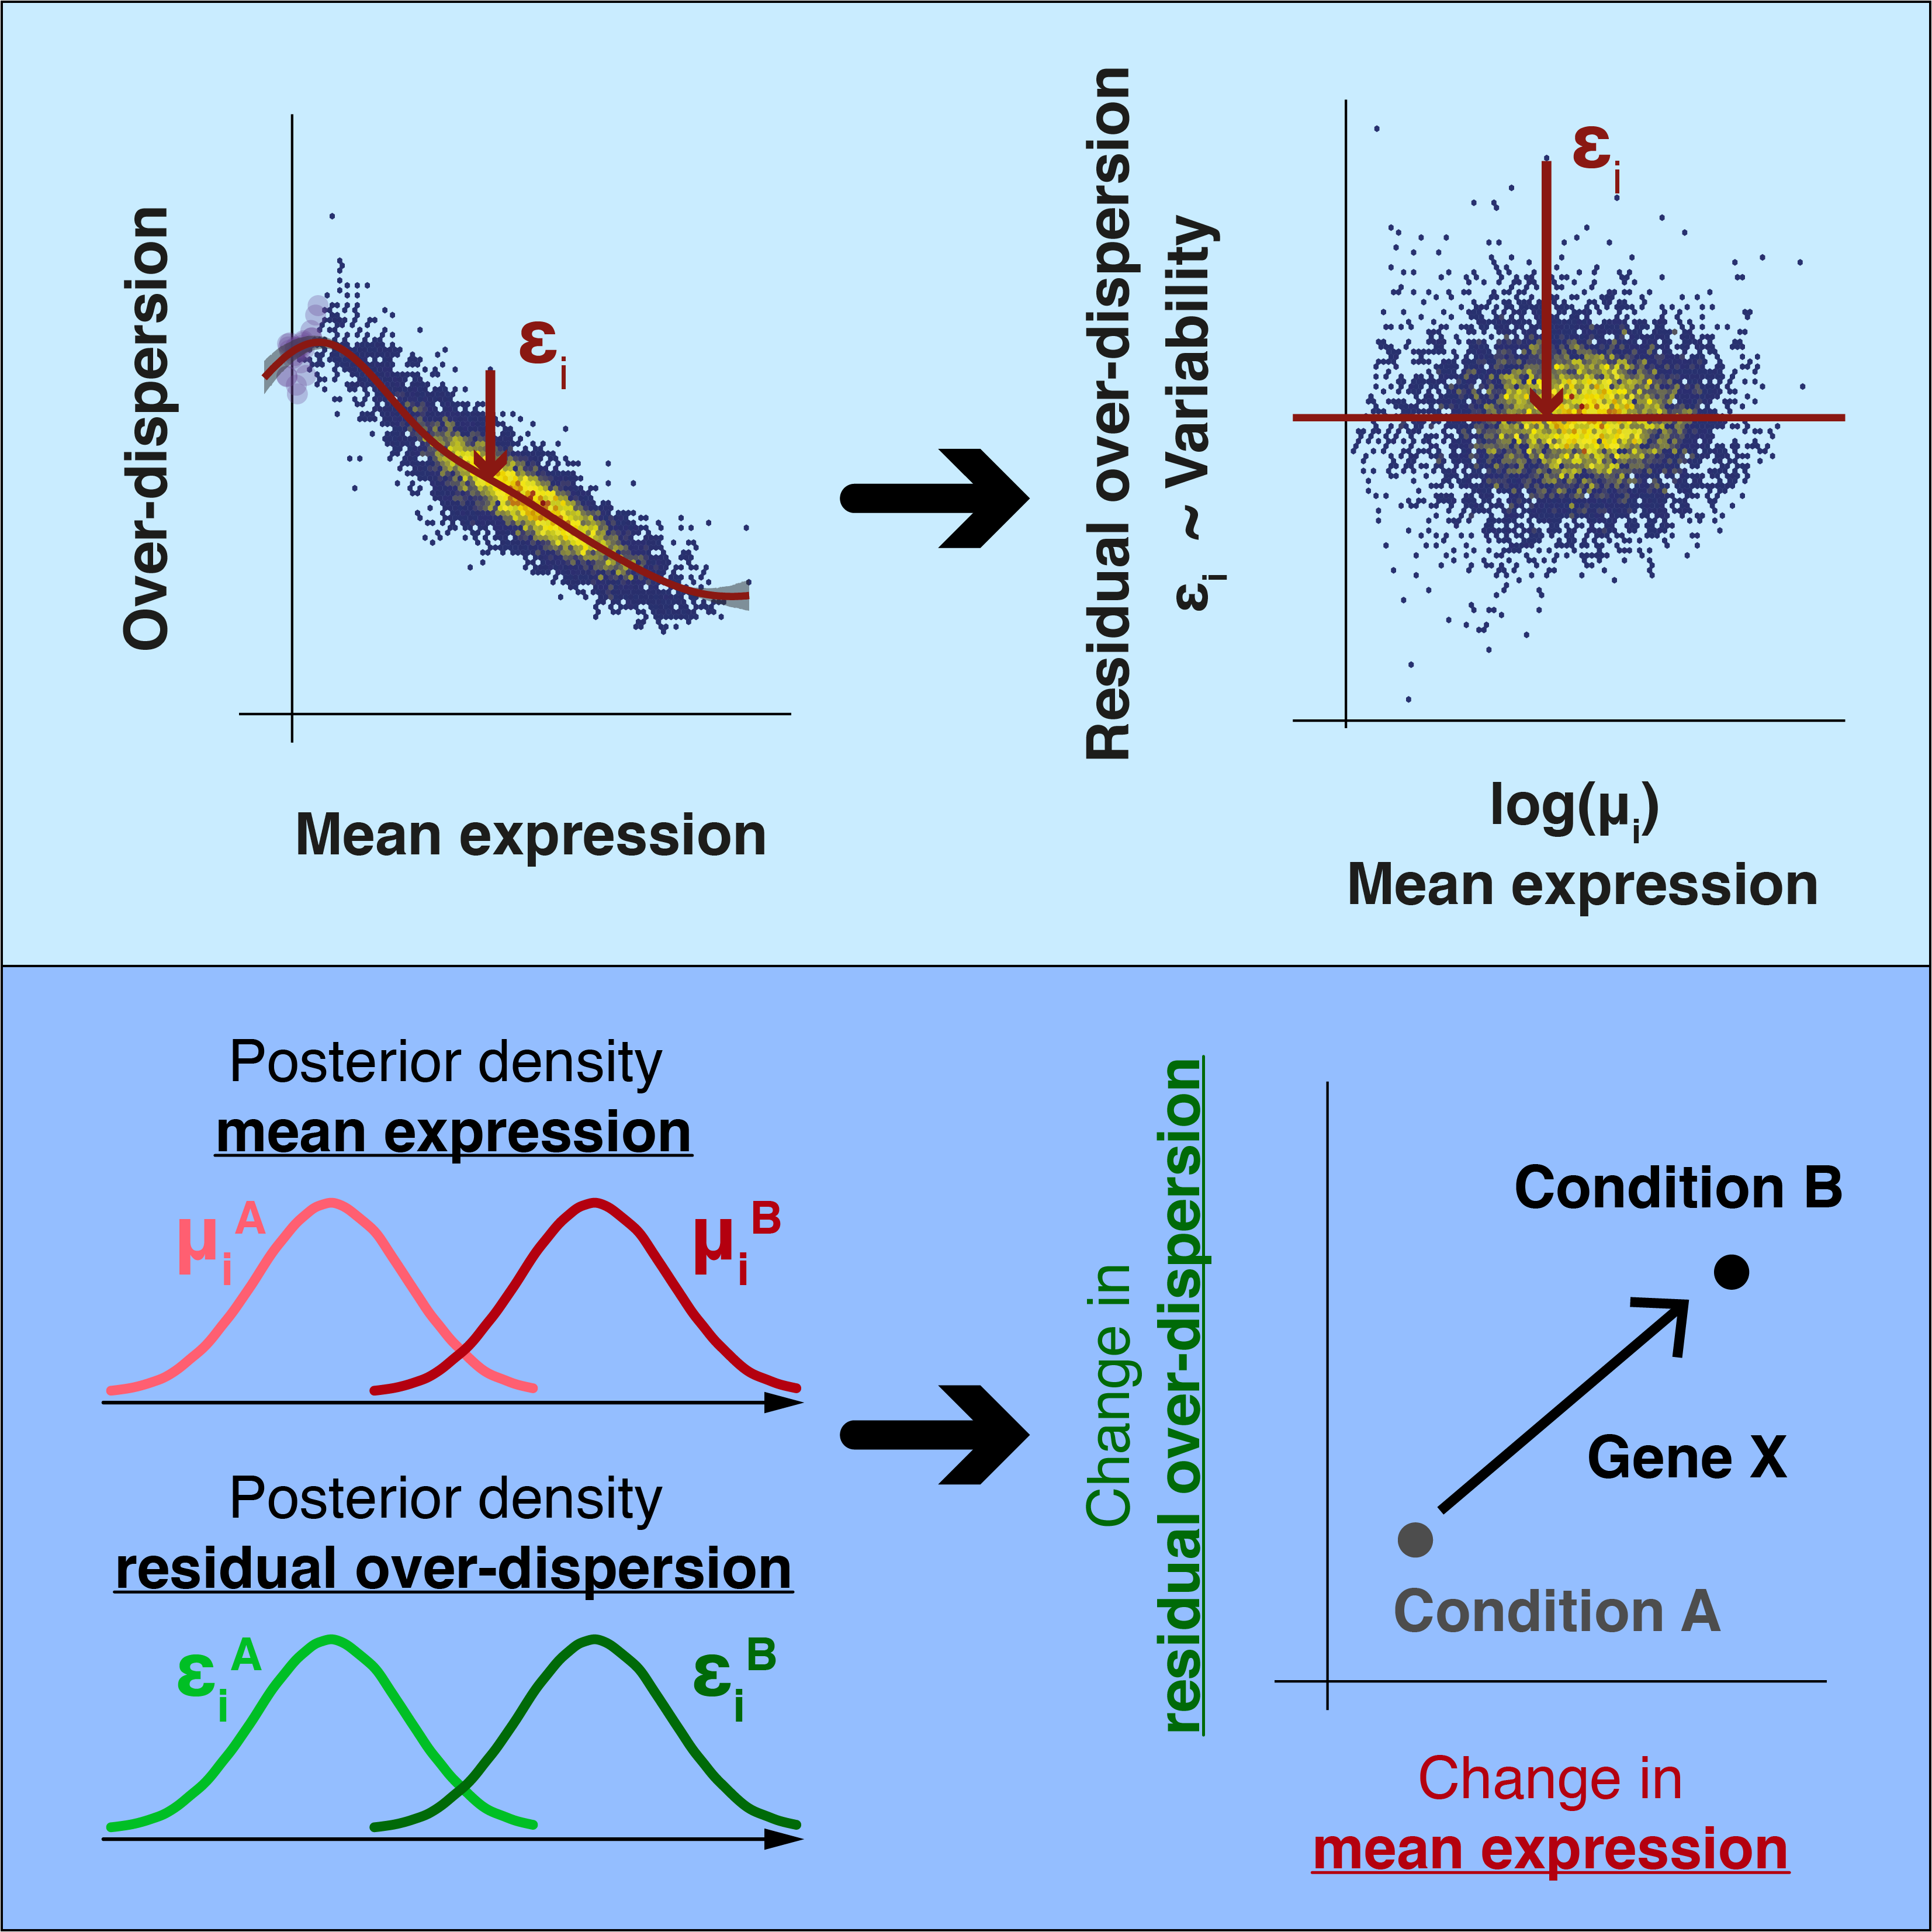
\includegraphics[width=0.5\textwidth]{GraphicalAbstract.png}
\end{figure}

\newpage

% Include different main sections of the first chapter
%!TEX root = ../chapter2.tex
%******************************
%	 Introduction 
%*****************************

\section{Introduction}

Ageing is characterised by the progressive decline of physiological and cellular functions \citep{Lopez-Otin2013, Booth2016}. 
Nine hallmarks of ageing have been described to determine the ageing phenotype: genomic instability, telomere attrition, epigenetic alterations, loss of proteostasis, de-regulated nutrient sensing, mitochondrial dysfunction, cellular senescence, stem cell exhaustion, and altered intercellular communication \citep{Lopez-Otin2013}. 
Ageing can have a complex and tissue-specific impact on gene expression levels \citep{Zahn2007}, as seen by microarray expression analyses of collections of mouse CD4\plus{} and CD8\plus{} T cells \citep{Mirza2011}, rat hepatocytes \citep{Tollet-Egnell2000}, mouse and human brain \citep{Lu2004, Lee2000}, human muscle \citep{Welle2003, Zahn2006}, human kidney \citep{Rodwell2004}, human retina \citep{Yoshida2002}, and different species of Drosophila and Caenorhabditis \citep{Mccarroll2004}. For instance, ageing affects distinct functional pathways, even in closely related CD4\plus{} and CD8\plus{} T cells \citep{Mirza2011}. \\

Transcriptional noise, RNA processing aberrations, impaired DNA repair, and chromosomal instability can be caused by epigenetic changes in DNA methylation, histone modifications and chromatin remodelling \citep{Lopez-Otin2013}. 
Global DNA methylation slightly decreases during ageing but increases in common disease-related genes over the lifespan of humans \citep{Talens2012}. 
In mice, around 35\% of assayed genes showed either increased or decreased DNA methylation over ageing, with substantial tissue-specificity \citep{Maegawa2010}. 
Similarly, ageing introduces changes in histone modifications such as the increase of activating \gls{H4K16ac} and \gls{H3K4me3}, and repressive \gls{H4K20me3}. 
Furthermore, ageing decreases the repressive \gls{H3K9me3} and \gls{H3K27me3} marks \citep{Han2012, Fraga2007}. 
One well studied system that controls cellular function is the \gls{Sir}2 histone deacetlyase, which is encoded by seven homologs in mammals \citep{Houtkooper2016}. 
The chromatin-associated protein SIRT6 in mice has been shown to protect genomic stability by promoting resistance to DNA damage. 
Loss of this protein induces ageing-realted phenotypes within 4 weeks of murine lifespan \cite{Mostoslavsky2006}. 
Similar effects can be seen for SIRT1 \cite{Oberdoerffer2008}.\\

While most studies focused on identifying age-associated gene expression profiles \citep{DeMagalhaes2009}, the role of transcriptional noise during ageing has only been sporadically assessed. 
Analysis of fifteen genes in terminally differentiated cardiomyocytes suggested that ageing can lead to increased cell-to-cell transcriptional variability \citep{Bahar2006}. 
In contrast, single-cell analysis of the transcription of six genes in four different haematopoietic cell types showed few cell-to-cell changes between old and young animals, suggesting that transcriptional variability may not be a universal attribute of ageing \citep{Warren2007}. 
Whether cell-to-cell gene expression variability increases during ageing on a genome-wide basis, particularly for dynamic activation programs, remains largely unexplored.\\

Single-cell RNA sequencing presents a powerful technology to quantify  transcriptional variability for thousands of genes across hundreds of cells simultaneously. 
For example, Kowalczyk \textit{et al.} performed a high-resolution scRNA-seq analysis of haematopoietic stem cells in young and old mice. 
Here, cell cycle is the primary driver for cell-to-cell variability in gene expression, and ageing decreases the entry of long-term haematopoietic stem cells into G1 phase in a cell type-specific manner \citep{Kowalczyk2015}.\\ 

To evaluate the impact of ageing on gene expression levels and cell-to-cell transcriptional variability, we selected CD4\plus{} T cells as model system. 
As explained in \textbf{Box 1} (page \pageref{box1}), transcriptional noise is defined as cell-to-cell variability in expression within a homogeneous population of cells. 
Naive CD4\plus{} T cells are readily isolated as single, phenotypically homogeneous cells when purified from young and aged spleens and can easily be stimulated into a physiologically-relevant, activated transcriptional state \emph{in vitro}. 
Furthermore, they are maintained in a quiescent state, but have the ability to respond to antigen stimulation with proliferation and effector differentiation, which is essential for life-long maintenance of adaptive immune function against infection and cancer \citep{Swain2012, Kim2014a}. 
With this, they sit at the root of adaptive immunity and disruption of their transcriptional programme can lead to severe phenotypes during ageing. \\

Previously, comparing gene expression levels in matched tissues from different mammalian species was used as a tool for revealing conserved cell-type-specific regulatory programmes \citep{Sudmant2015, Finseth2014, Brawand2011, Flajnik2009}. 
For instance, a conserved set of response genes has been identified by comparison of bulk gene expression between human and mouse CD4\plus{} T cells after immune activation \citep{Shay2013}. 
So far, it is not known whether conservation of gene expression levels is also reflected in cell-to-cell variability.\\

Here, we dissected the activation dynamics of naive CD4\plus{} T cells at the single cell level during ageing in two sub-species of mice. 
With this, we assayed transcriptional dynamics during immune response and how ageing possibly perturbs this system. 
By comparing our findings across divergent strains of mice, we assessed the evolutionary conservation of the immune response and ageing phenotype. 
Furthermore, we isolated pure naive and effector memory CD4\plus{} T cells to profile age-related changes in different CD4\plus{} T cell subsets.

\newpage
%!TEX root = ../chapter2.tex
%******************************
%	 Results 
%*****************************

\section{Extending the  BASiCS model}

Unlike bulk RNA sequencing, scRNA-Seq provides information about cell-to-cell expression heterogeneity within a population of cells. Past works have used a variety of measures to quantify this heterogeneity. Among others, this includes the coefficient of variation \citep[CV,][]{Brennecke2013} and entropy measures \citep{Richard2016}. The BASiCS model \citep{Vallejos2015BASiCS, Vallejos2016} which was introduced in section \ref{sec0:BASiCS} focuses on biological \textit{over-dispersion} as a proxy for transcriptional heterogeneity. This is defined by the excess of variability that is observed with respect to what would be predicted by Poisson sampling noise, after accounting for technical variation. 

\subsection{The BASiCS model}

As a reminder: Let $X_{ij}$ be a random variable representing the expression count of gene $i$ ($ \in \{1, \ldots, q\}$) in cell $j$ ($\in \{ 1, \ldots ,n\}$).  To control for technical noise, we employ reads from synthetic RNA spike-ins (see \citep{Jiang2011}). We assume the first $q_0$ genes to be biological followed by the $q-q_0$ spike-in genes. BASiCS assumes a hierarchical Poisson formulation: 

\begin{equation} \label{eq::PoissonBASiCS}
 X_{ij}|\mu_i,\phi_j,\nu_j,\rho_{ij} \ind
 \left\lbrace
  \begin{aligned}
    &\text{Poisson}(\phi_j\nu_j\mu_i\rho_{ij}), && i=1,...,q_0,j=1,...n;  \\ 
    &\text{Poisson}(\nu_j\mu_i), && i=q_0+1,...,q,j=1,...,n,    	    
  \end{aligned}
\right.
\end{equation} 

where, to account for technical ($\nu_j$) and biological ($\rho_ij$) factors that affect the variance of the transcript counts, we incorporate two random effects: 

\begin{equation} \label{eq::RandomEffectsBASiCS}
\nu_j|s_j,\theta \ind \text{Gamma}\left(\frac{1}{\theta},\frac{1}{s_j\theta}\right), \hspace{0.5cm} \rho_{ij}|\delta_i  \ind \text{Gamma}\left(\frac{1}{\delta_i},\frac{1}{\delta_i}\right)\\
\end{equation} 

Here, $\phi_j$ represents a cell-specific normalization parameter to correct for differences in mRNA content between cells and $s_j$ models cell-specific scale differences affecting all biological and technical genes. The strength of the technical noise $\nu_j$ noise is quantified by a global parameter $\theta$ (shared across all genes and cells). The strength of heterogeneous gene expression across cells $\rho_{ij}$ is controlled by gene-specific over-dispersion parameters $\delta_i$ which we used as a proxy for biological expression variability in the previous chapter.  Finally, gene-specific parameters $\mu_i$ represent average expression of a gene across cells. \\

As shown in the previous chapter, over-dispersion as a measure of variability can be used to identify genes whose transcriptional heterogeneity differs between groups of cells (defined by experimental conditions or cell types). However, the strong relationship that is typically observed between variability and mean estimates (see \textbf{Section \ref{sec0:BASiCS}} and \citep{Brennecke2013}) can hinder the interpretation of these results. 

\newpage

\subsection{Approaches to correct the mean-variability confounding effect}

A simple solution to avoid this confounding was used in the previous chapter by restricting the assessment of differential variability to genes with equal mean expression across populations \textbf{(Fig.~\ref{fig2:Schematic_model}A and Section \ref{sec1:BASiCS})}. However, this is sub-optimal, particularly in the case of naive and activated CD4\plus{} T cells where large sets of genes are differnetially regulated upon immune activation. With the current model, immune response genes (e.g.~cytokines, nuclear receptors, transcription factors) are excluded from differential variability testing. An alternative approach is to directly adjust variability measures to remove this confounding. For example, \cite{Kolodziejczyk2015cell} computed the empirical distance between the squared CV to a rolling median along expression levels --- referred to as the DM method.  \\

In line with this idea, our method extends the statistical model implemented in BASiCS \citep{Vallejos2015BASiCS, Vallejos2016} to meaningfully assess changes in transcriptional heterogeneity when genes exhibit shifts in mean expression \textbf{(Fig.~\ref{fig2:Schematic_model}B)}. For this, we infer a regression trend between over-dispersion ($\delta_i$) and gene-specific mean parameters ($\mu_i$), by introducing a joint informative prior to capture the dependence between these parameters. A latent gene-specific \textit{residual over-dispersion} parameter $\epsilon_i$ describes departures from this trend \textbf{(Fig~\ref{fig2:Schematic_model}C)}. The value of $\epsilon_i$ indicates whether a gene exhibits more (positive) or less (negative) variation than expected relative to genes with similar expression levels. Importantly, this measure is not confounded by mean expression \textbf{Fig.~\ref{fig2:Schematic_model}D}. \\

The hierarchical Bayes approach infers full posterior distributions for the gene-specific latent residual over-dispersion parameters $\epsilon_i$. As a result, we can directly use a probabilistic approach to identify genes with large absolute differences in residual over-dispersion between two groups of cells. When the posterior samples of $\epsilon_i$ in condition A are very different from posterior samples of $\epsilon_i$ in condition B, the majority of values for $|\epsilon_i^A - \epsilon_i^B|$ are larger than a given threshold $\psi_0>0$. In this case, the gene is found to be differentially variable between the two conditions  \textbf{(Fig.~\ref{fig2:Schematic_model}E and Section \label{sec0:decision})}. In contrast, mean-corrected point estimates for residual noise parameters (such as those obtained by the DM method) cannot be directly used to perform gene-specific statistical testing between two conditions as no measure of the uncertainty in the estimate is readily available.\\

\newpage

\begin{figure}[!h]
\centering
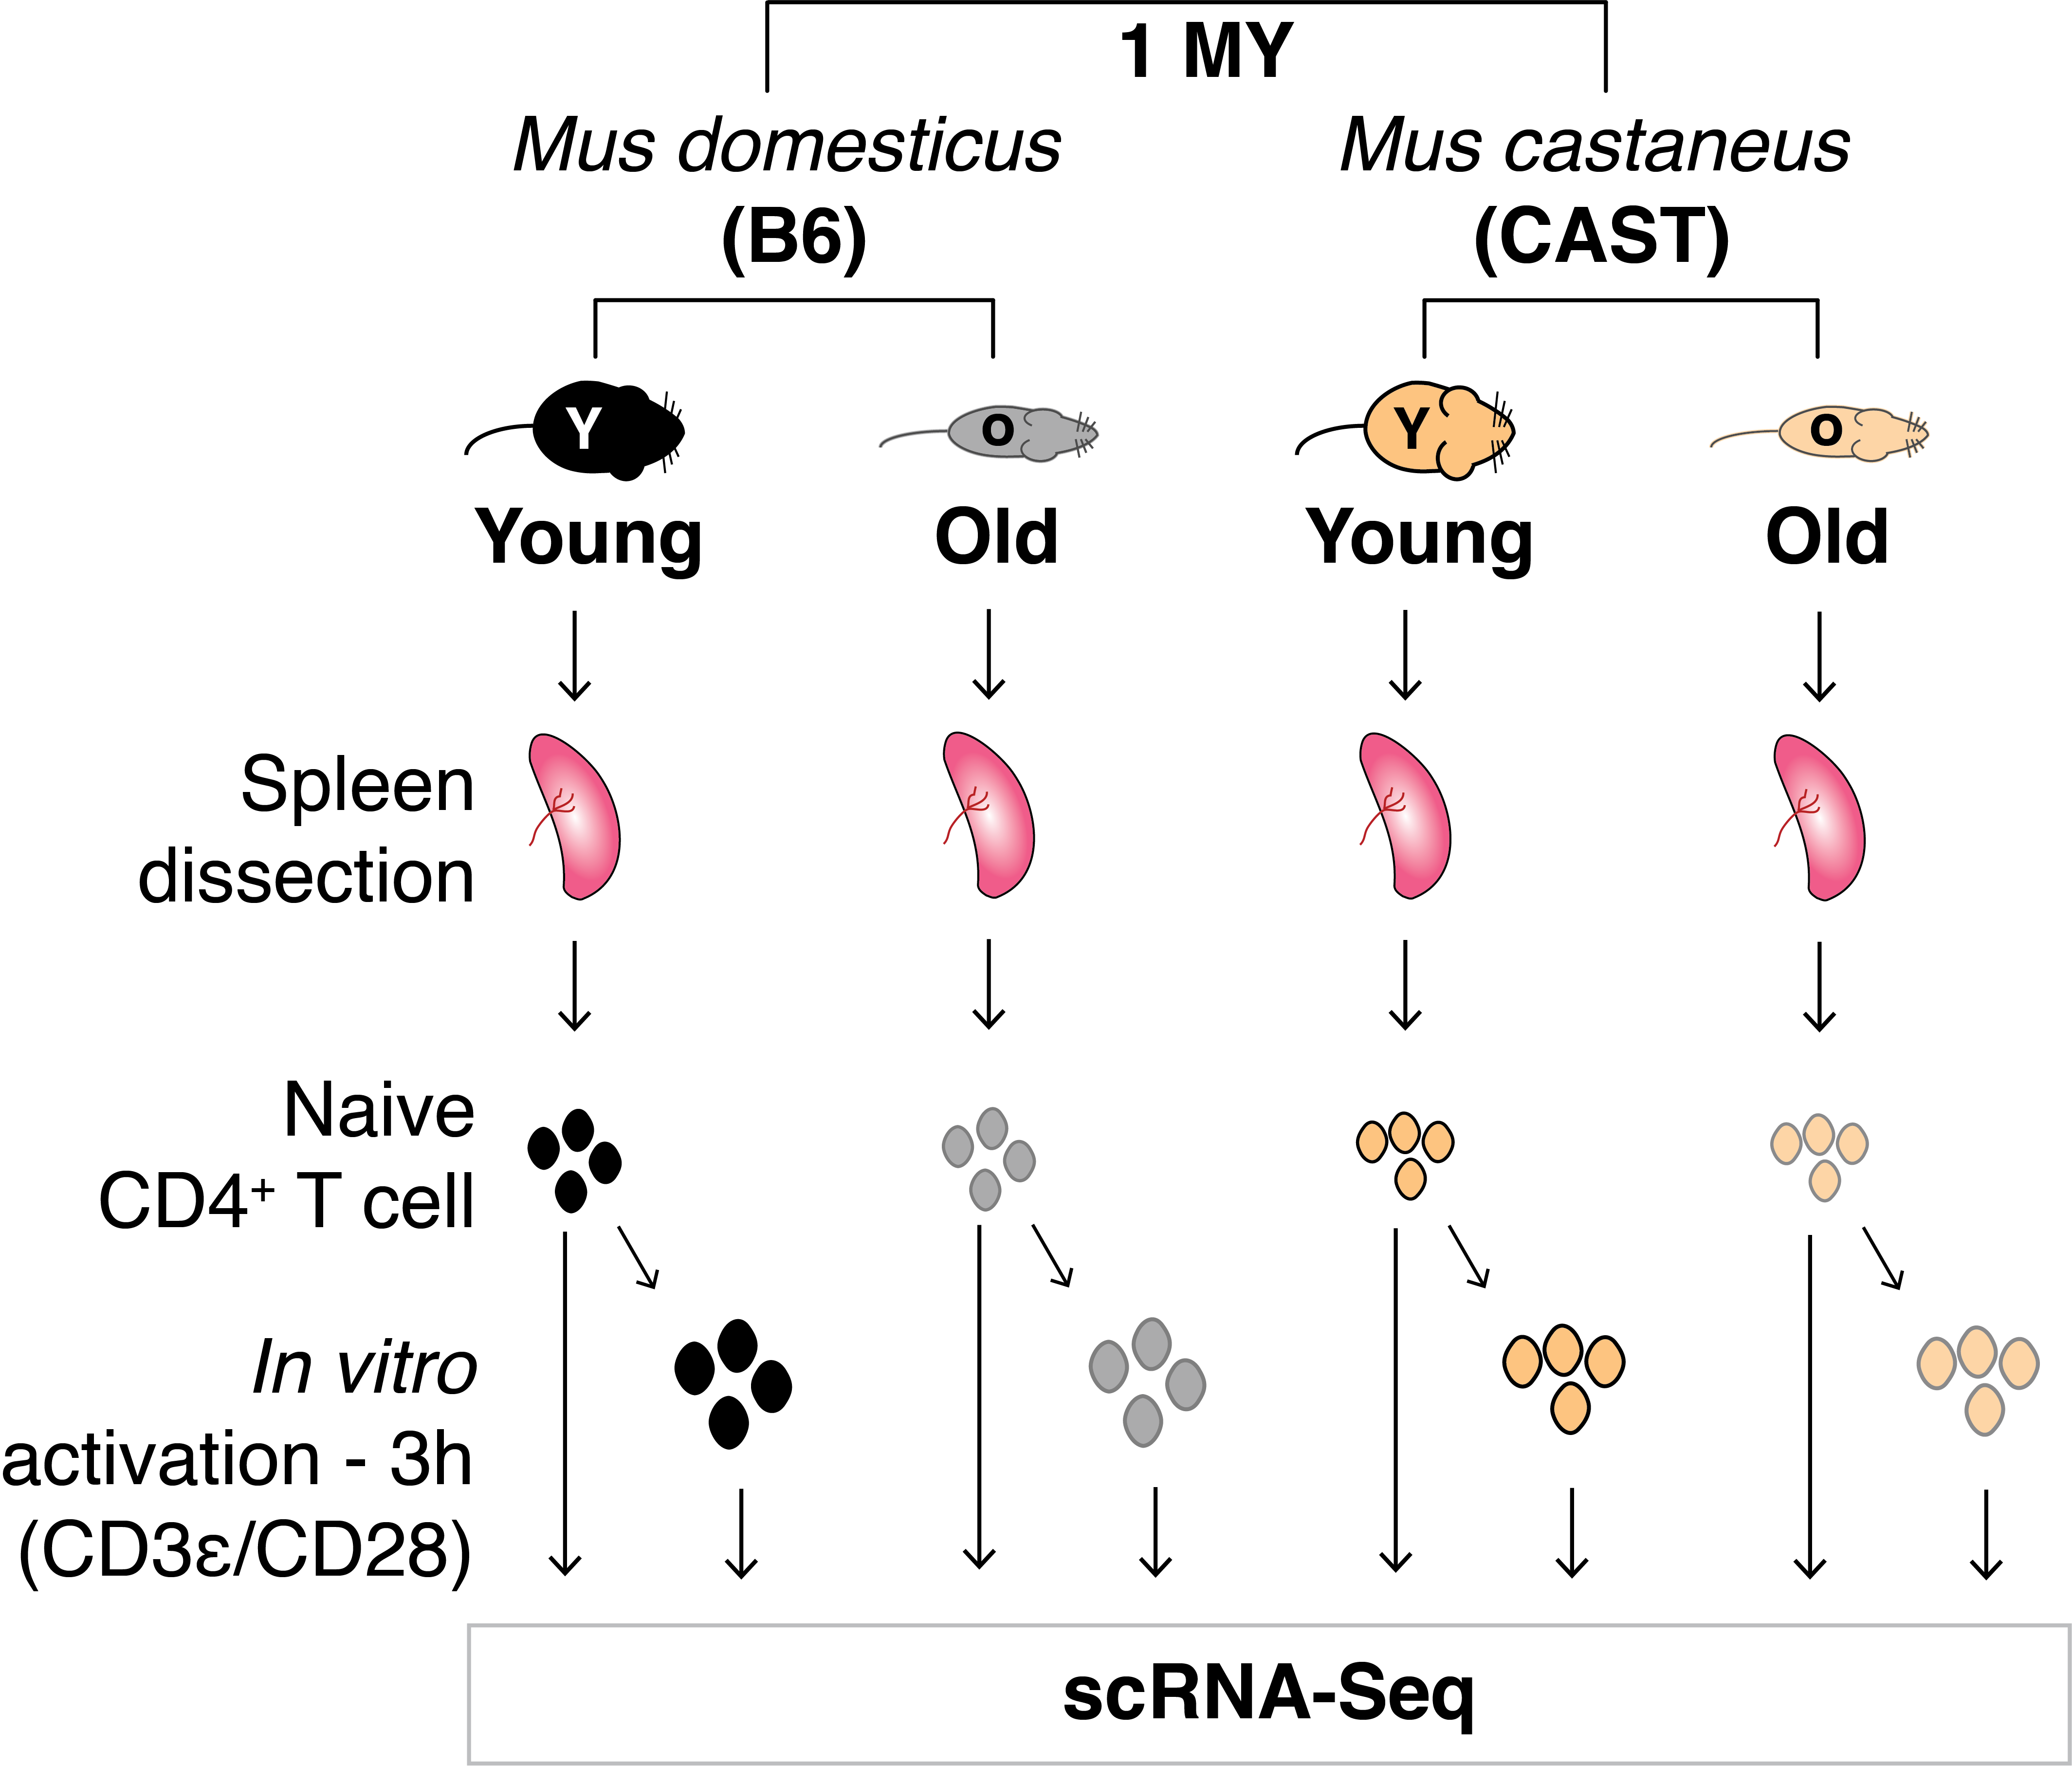
\includegraphics[width=0.9\textwidth]{Fig_1.png}
\caption[Addressing the mean confounding effect in scRNA-Seq data]{\textbf{Addressing the mean confounding effect in scRNA-Seq data (full legend on next page).}\\}
\label{fig2:Schematic_model}
\end{figure}

\newpage

\captionsetup[figure]{list=no}
\addtocounter{figure}{-1}   
\captionof{figure}{\textbf{Addressing the mean confounding effect in scRNA-Seq data (continued).}\\
\textbf{(A and B)} Illustration of changes in expression variability for a single gene between two cell populations without (left) and with (right) changes in mean expression, \textbf{(C and D)} The extended BASiCS model infers a regression trend between gene-specific estimates of over-dispersion parameters $\delta_i$ and mean expression $\mu_i$. Residual over-dispersion parameters $\epsilon_i$ are defined by departures from the regression trend (red arrow). The colour code within the scatterplots is used to represent areas with high (yellow/red) and low (blue) concentration of genes. For illustration purposes, the data introduced by \cite{Antolovic2017} has been used, \textbf{(C)} Illustration of the typical confounding effect that is observed between gene-specific estimates of over-dispersion parameters $\delta_i$ and mean expression parameters $\mu_i$. Genes that are not detected in at least 2 cells are indicated by purple points, \textbf{(D)} Gene-specific estimates of residual over-dispersion parameters $\epsilon_i$ are independent of mean expression parameters $\mu_i$, \textbf{(E)} Illustration of how posterior uncertainty is used to highlight changes in residual over-dispersion. Two example genes with (upper panels) and without (lower panels) changes in residual over-dispersion are shown. Left panels illustrate the posterior density associated to residual over-dispersion parameters $\epsilon_i$ for a gene in two groups of cells (group A: light blue, group B: dark blue). The coloured area in the right panels represents the posterior probability of observing an absolute difference $|\epsilon^A_{i} - \epsilon^B_{i}|$ that is larger than the minimum tolerance threshold $\psi_0$.\\}
\captionsetup[figure]{list=yes}

\subsection{Modelling the confounding between mean and over-dispersion} \label{sec2:extended_BASiCS}

Here, we extend BASiCS to account for the confounding effect described above. In a Bayesian framework, the prior information captures the relationship between parameters. Therefore, we introduce the following joint prior distribution for $(\mu_i, \delta_i)'$: 

\begin{equation} \label{eq::jointprior} \mu_i \sim \text{log-Normal}\left(0, s^2_{\mu}\right), \hspace{0.8cm}
\delta_i | \mu_i \sim \text{log-}\text{T}_{\eta}\left( \text{f}(\mu_i), \sigma^2 \right).
\end{equation} 

The latter is equivalent to the following non-linear regression model:

\begin{equation} \label{eq::regression}
\log(\delta_i) =\text{f}(\mu_i)+\epsilon_i, \hspace{0.5cm} \epsilon_i \sim{}\text{T}_{\eta}(0,\sigma^2), 
\end{equation} where $\text{f}(\mu_i)$ represents the over-dispersion (on the log-scale) that is predicted by the global trend (across all genes) for a given mean expression $\mu_i$. Therefore, $\epsilon_i$ can be interpreted as a latent gene-specific \textit{residual over-dispersion} parameter, capturing departures from the overall trend. \\

A similar approach was introduced by DESeq2 \citep{Love2014} in the context of bulk RNA sequencing. Whereas DESeq2 assumes normally distributed errors when estimating this trend, here we use Student-T distributed errors as it leads to inference that is more robust to the presence of outlier genes. 

\newpage

Moreover, the parametric trend assumed by DESeq2 is replaced by a more flexible semi-parametric approach. This is defined by

\begin{equation} \label{eq::trend}
\text{f}(\mu_i) = \alpha_0 + \log(\mu_i)\alpha_1 + \sum_{l=1}^L \text{g}_l(\log(\mu_i))\beta_l,
\end{equation} 

which is a linear combination of an intercept, a linear term $\log{\mu_i}$ and a set of $L$ Gaussian radial basis function (GRBF) kernels $\text{g}_1(\cdot), \ldots, \text{g}_L(\cdot)$. As in \cite{Kapourani2016}, these are defined as: 

\begin{equation} \label{eq::GRBF}
\text{g}_l(\log(\mu_i)) = \exp\left\lbrace-\frac{1}{2}\left(\dfrac{\log(\mu_i)-m_l}{h_l}\right)^2\right\rbrace, \hspace{0.3cm} l = 1, \ldots, L,
\end{equation} 

where $m_l$ and $h_l$ represent location and scale hyper-parameters for GRBF kernels and $\alpha_0, \alpha_1, \beta_1, \ldots, \beta_L$ are regression coefficients. \\

In \eqref{eq::trend}, the linear term captures the (typically negative) global correlation between $\delta_i$ and $\mu_i$. Its addition also stabilises inference of GRBFs around mean expression values where only a handful of genes are observed. In \eqref{eq::GRBF}, the location and scale hyper-parameters $(m_l, h_l)$ are assumed to be fixed \emph{a priori}. A schematic representation of this regression approach can be seen in \textbf{Fig. \ref{fig2:GRBFs}}.

\begin{figure}[!h]
\centering
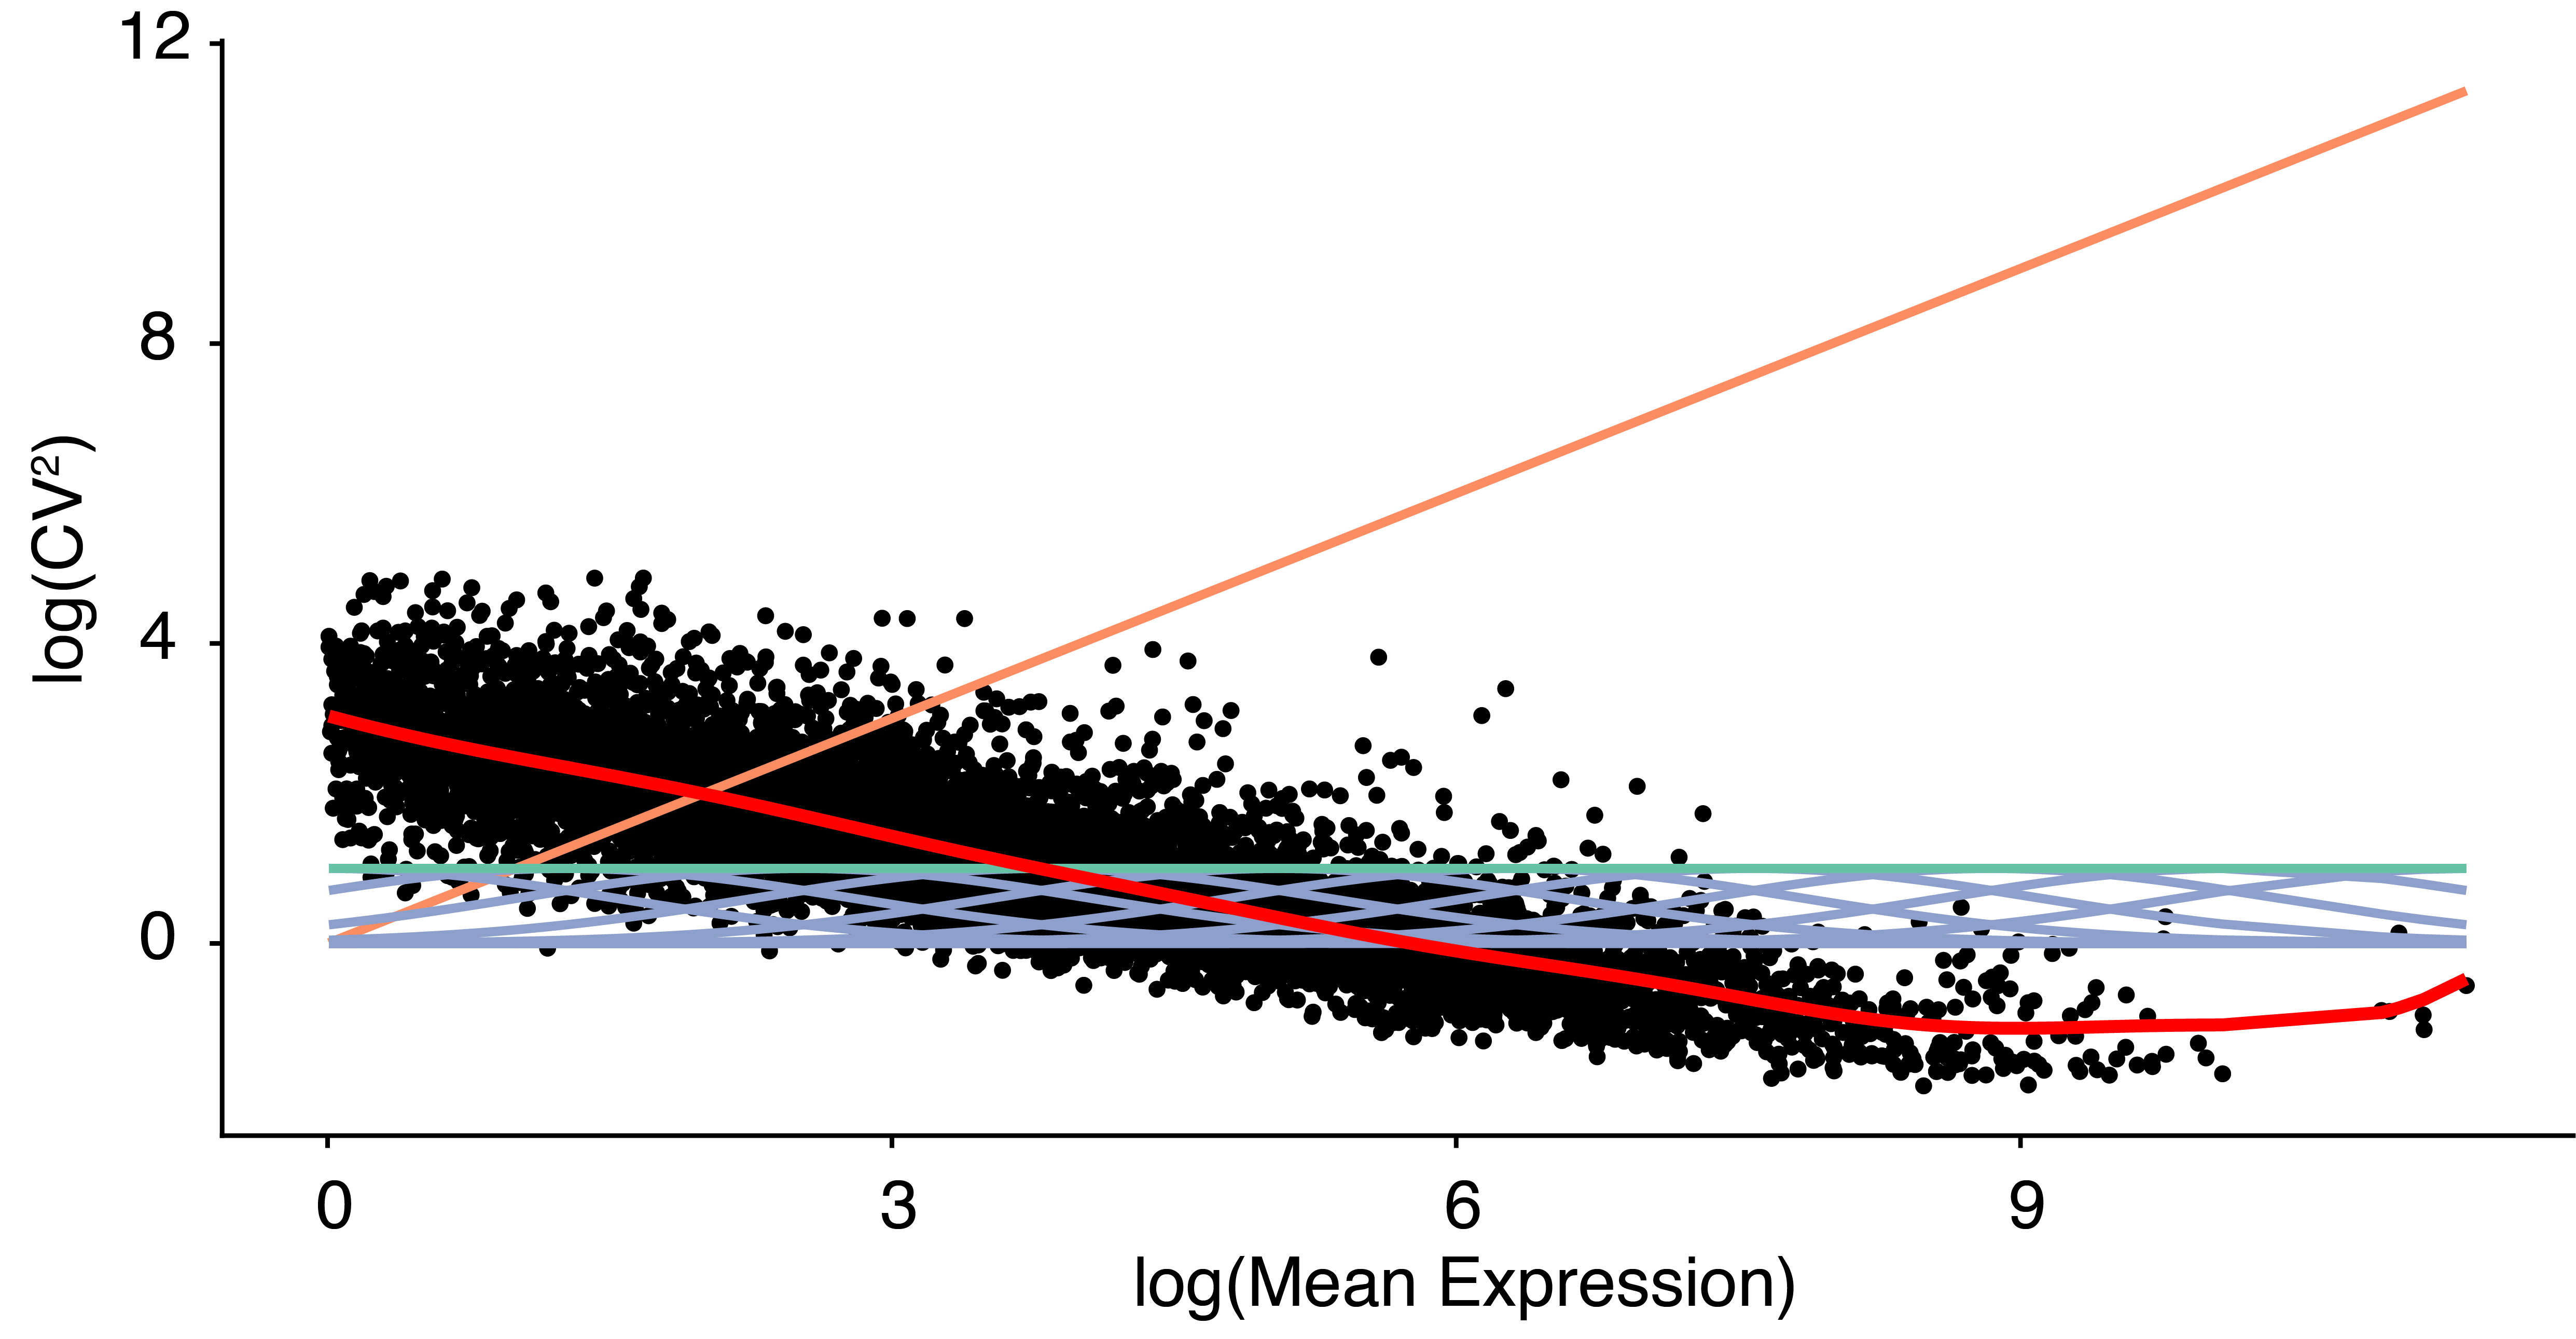
\includegraphics[width=0.9\textwidth]{Fig_2.png}
\caption[Schematic representation of the regression approach using GRBFs]{\textbf{Schematic representation of the regression approach using GRBFs.}\\
Point estimates of the squared coefficient of variation (CV$^2$) were plotted against mean expression. For fitting a regression trend, the model matrix $X$ contains an intercept term (green line), a linear component (orange line) and 10 GRBFs (blue lines). For visualization purposes, a linear regression was fitted using least-square estimates (red line) based on the given model matrix $X$ and data from Dictyostelium at day 0 \citep{Antolovic2017}.}
\label{fig2:GRBFs}
\end{figure}


\subsection{Implementation}

Next, we will give a detailed explanation on how the model was build and how posterior sampling was performed.  


\subsubsection{Prior specification}

For implementation purposes, the log-Student-T distribution in \ref{eq::jointprior} is represented via a shape mixture of a log-Normal density with a Gamma density as in \cite{Vallejos2015}. This introduces an auxiliary set of parameters $\lambda_i$ such that the full prior specifications of the extended BASiCS model are:

\begin{align*}
\mu_i &\ind \mbox{log-Normal}\left(0, s^2_{\mu}\right) \\
\delta_i| \mu_i,\beta,\sigma^2, \lambda_i, \eta &\ind \text{log-N}\left( \text{f}(\mu_i),\frac{\sigma^2}{\lambda_i} \right)\\
\lambda_i|\eta &\ind \text{Gamma}\left(\frac{\eta}{2},\frac{\eta}{2}\right)\\
\beta|\sigma^2 & \sim \textnormal{Normal}(m_\beta,\sigma^2V_\beta),\\
\sigma^2 & \sim  \textnormal{Inv-Gamma}(a_{\sigma^2},b_{\sigma^2}),\\
s_j & \iid  \textnormal{Gamma}(a_s,b_s) \\
(\phi_1, \ldots, \phi_n)' & \sim  n \times \textnormal{Dirichlet}(a_\phi),\\
\theta & \sim  \textnormal{Gamma}(a_\theta,b_\theta)
\end{align*}

Here, $s^2_{\mu}, m_\beta, V_\beta, a_{\sigma^2}, b_{\sigma^2}, a_s, b_s, a_\phi, a_\theta, b_\theta$ are hyper-parameters that are fixed \emph{a priori}. Their initial values can be found in \textbf{Appendix \ref{appB.1.hyper}}. In principle, the degrees of freedom parameter $\eta$ could also be estimated within a Bayesian framework. However, we observed that fixing this parameter \emph{a priori} led to more stable results. A default choice for this parameter is described in \textbf{Section \ref{sec2:hyper-parameters}}.

\newpage

\subsubsection{Estimation of regression parameters}

To simplify inference for the regression coefficients $\beta = (\alpha_0, \alpha_1, \beta_1, \ldots, \beta_L)'$ equation \ref{eq::trend} can be rewritten as a linear regression model using 

\begin{equation} \label{eq::trend2} 
\text{f}(\mu_i) = X \beta
\end{equation} 

Here, $X$ is a $q_0 \times (L+2)$ model matrix given by 

\begin{equation} \label{eq::X} X = \left( \begin{array}{ccccc}
1 & \log(\mu_1) & g_1(\log(\mu_1)) & \cdots & g_L(\log(\mu_1)) \\
1 & \log(\mu_2) & g_1(\log(\mu_2)) & \cdots & g_L(\log(\mu_2)) \\
\vdots & \vdots & \vdots & \ddots & \vdots  \\
1 & \log(\mu_{q_0}) & g_1(\log(\mu_{q_0})) & \cdots & g_L(\log(\mu_{q_0}))
\end{array}\right)
\end{equation}

Each column contains either the intercept, the linear component or values of one of the $L$ GRBF. This matrix is updated every 50 iterations during posterior sampling.

\subsubsection{Posterior inference}

Posterior inference for the model described above is implemented by extending the Adaptive Metropolis within Gibbs sampler \citep{Roberts2009} that was adopted by Vallejos \emph{et al.} 2016 \cite{Vallejos2016}. To implement the sampler, the full conditionals for each model parameter need to be derived. \\

As in Vallejos \emph{et al.}, 2015 \cite{Vallejos2015BASiCS}, the random effect $\rho_{ij}$ in \ref{eq::PoissonBASiCS} is integrated out, leading to following count distributions:

\begin{equation} \label{eq::NegBinBASiCS}
 X_{ij}|\mu_i,\delta_i,\phi_j,\nu_j \ind
 \left\lbrace
  \begin{aligned}
    &\text{Neg-Bin}\left(\frac{1}{\delta_i},\frac{\phi_j\nu_j\mu_i}{\phi_j\nu_j\mu_i+\frac{1}{\delta_i}}\right), && i=1,...,q_0,j=1,...n;  \\ 
    &\text{Poisson}(\nu_j\mu_i), && i=q_0+1,...,q,j=1,...,n        
  \end{aligned}
\right.
\end{equation}

Based on \ref{eq::NegBinBASiCS}, the likelihood function therefore takes the form

\begin{align} \label{eq::loglik}
\Lagr = & \left[\prod_{i=1}^{q_0}\prod_{j=1}^n\frac{\Gamma(x_{ij}+\frac{1}{\delta_i})}{\Gamma(\frac{1}{\delta_i})x_{ij}!}\left(\frac{\frac{1}{\delta_i}}{\phi_j\nu_j\mu_i+\frac{1}{\delta_i}}\right)^\frac{1}{\delta_i}\left(\frac{\phi_j\nu_j\mu_i}{\phi_j\nu_j\mu_i+\frac{1}{\delta_i}}\right)^{x_{ij}}\right] \nonumber\\ 
&\times\left[\prod_{i=q_0+1}^{q}\prod_{j=1}^n\frac{(\nu_j\mu_i)^{x_{ij}}}{x_{ij}!}\exp\lbrace-\nu_j\mu_i\rbrace\right]\times{}\left[\prod_{j=1}^n\frac{(s_j\theta)^{-\frac{1}{\theta}}}{\Gamma(\frac{1}{\theta})}\nu_j^{\frac{1}{\theta}-1}\exp\left\lbrace-\frac{\nu_j}{s_j\theta}\right\rbrace\right]
\end{align} 

\newpage

The full conditionals can now be derived by calculating the parameter-dependent part of the posterior distribution which is a product of the likelihood times the prior specifications $\pi^\ast(\cdot)\propto{}\Lagr\times\pi(\cdot)$. Full conditionals for the model as as follows: 

Let $\text{f}(\mu_i)$ be as in \ref{eq::trend}. The full conditionals associated to the mean expression parameters $\mu_i$ and over-dispersion parameters $\delta_i$ are respectively given by:\\

\begingroup
\addtolength{\jot}{0.8em}
\begin{align*} \label{eq::FullCond}
&\pi^*(\mu_i|\cdot) && \propto \frac{\mu_i^{\sum_{j=1}^n{}x_{ij}}}{\prod_{j=1}^n{}(\phi_j\nu_j\mu_i+\frac{1}{\delta_i})^{\frac{1}{\delta_i}+x_{ij}}}\times{}\exp\left(-\frac{(\log(\mu_i))^2}{2a_\mu^2}-\frac{\lambda_i(\log(\delta_i)-f(\mu_i))^2}{2\sigma^2}\right)\frac{1}{\mu_i} \\
&\pi^*(\delta_i|\cdot) && \propto \left[\prod_{j=1}^n\frac{\Gamma(x_{ij}+\frac{1}{\delta_i})}{\Gamma(\frac{1}{\delta_i})}\frac{(\frac{1}{\delta_i})^{\frac{1}{\delta_i}}}{(\phi_j\nu_j\mu_i+\frac{1}{\delta_i})^{\frac{1}{\delta_i}+x_{ij}}}\right]\times{}\exp\left\lbrace-\frac{\lambda_i(\log(\delta_i)-f(\mu_i))^2}{2\sigma^2}\right\rbrace\frac{1}{\delta_i}\\
&\pi^*(\beta|\cdot)&&\propto{}\text{Normal}(m^*_\beta,\sigma^2V^*_\beta)\\
&\pi^*(\lambda_i|\cdot)&&\propto{}\text{Gamma}(a^*_\lambda,b^*_\lambda)\\
&\pi^*(\sigma^2|\cdot)&&\propto{}\text{Inv-Gamma}(a^*_{\sigma^2},b^*_{\sigma^2})\\
&\pi^*(s_j|\cdot)&&\propto{}s_j{}^{a_s-\frac{1}{\theta}-1}\exp\lbrace-\frac{\nu_j}{s_j\theta}-b_ss_j\rbrace\\
&\pi^*(\phi_j|\cdot)&&\propto{}\frac{\prod_{i=1}^{q_0}\phi_j{}^{\sum_{j=1}^nx_{ij}}}{\prod_{i=1}^{q_0}\prod_{j=1}^{n}(\phi_j\nu_j\mu_i+\frac{1}{\delta_i})^{\frac{1}{\delta_i}+x_{ij}}}\times{}\pi(\phi_j)\\
&\pi^*(\nu_j|\cdot)&&\propto{}\left[\prod_{i=1}^{q_0}\left(\frac{1}{\phi_j\nu_j\mu_i+\frac{1}{\delta_i}}\right)^\frac{1}{\delta_i}\left(\frac{\nu_j}{\phi_j\nu_j\mu_i+\frac{1}{\delta_i}}\right)^{x_{ij}}\right]\left[\prod_{i=q_0+1}^{q}\nu_j{}^{x_{ij}}\exp\lbrace-\nu_j\mu_i\rbrace\right]\nu_j^{\frac{1}{\theta}-1}\exp\lbrace-\frac{\nu_j}{s_j\theta}\rbrace\\
&\pi^*(\theta|\cdot)&&\propto{}\frac{\left(\prod_{j=1}^{n}\frac{s_j}{\nu_j}\right)^{-\frac{1}{\theta}}}{\Gamma{}^n(\frac{1}{\theta})}\theta^{a_\theta-\frac{n}{\theta}-1}\exp\lbrace-\frac{1}{\theta}\sum_{j=1}^n\frac{\nu_j}{s_j}-b_\theta\theta\rbrace
\end{align*}
\endgroup

Here, posteriors for $\beta, \lambda_i, \sigma^2$ take on closed form distributions. The posterior for $s_j$ represents a Generalized Inverser Gaussian distribution with parameters. To sample all other posterior distributions adaptive Metropolis sampling was implemented as described in \textbf{Section \ref{sec0:posterior_inference}}. The derivation of the full conditionals can be found in \textbf{Appendix  \ref{appB.1.derivation}}. In practice, the MCMC sampler is run for 40,000 iterations with a 20,000 iteration burn in period. The chain was thinned by storing parameter samples every 20 iterations.

\newpage

\subsection{Probabilistic rule associated to the differential test} \label{sec:differentialtest}

The residual over-dispersion parameter is calculated as $\epsilon_i=\log(\delta_i)-\text{f}(\mu_i)$. We can now implement a probabilistic approach to identify changes in residual over-disperison between groups of cells. Let $\delta_i^A$ and $\delta_i^B$ be the over-dispersion parameters associated to gene $i$ in groups $A$ and $B$. Following \ref{eq::regression}, the log$_2$ fold change in over-dispersion between these groups can be decomposed as: 

\begin{equation} \label{eq::dispersion_lfc}
\log_2 \left( \frac{\delta_i^A}{\delta_i^B}\right) = \log_2(e) \times \left[\underbrace{\text{f}^A(\mu_i^A) - \text{f}^B(\mu_i^B) }_{\text{Mean contribution}} + \underbrace{\epsilon_i^A - \epsilon_i^B}_{\text{Residual change}} \right]
\end{equation} 

where the first term captures the over-dispersion change that can be attributed to differences between $\mu_i^A$ and $\mu_i^B$. The second term in \ref{eq::dispersion_lfc} represents the change in residual over-dispersion that is not confounded by mean expression. Based on this observation, statistically significant differences in residual over-dispersion will be identified for those genes where the tail posterior probability of observing a large difference between $\epsilon_i^A$ and $\epsilon_i^B$ exceeds a certain threshold $\psi_0 > 0$:

\begin{equation} \label{eq::decision_rule}
\pi_i(\psi_0)\text{P}(\mid\epsilon_i^{A}-\epsilon_i^{B}\mid >\psi_0 \mid \text{Data} ) >\alpha_R
\end{equation}
 
As a default choice, we assume $\psi_0 = \log_2(1.5) / \log_2(e) \approx 0.41$ which translates into a 50\% increase in over-dispersion. In the limiting case when $\psi_0 = 0$, the probability in \eqref{eq::decision_rule} is equal to 1 regardless of the information contained in the data. Therefore, as in \cite{Bochkina2007}, our decision rule is based on the maximum of the posterior probabilities associated to the one-sided hypotheses $\epsilon^A - \epsilon^B_i > 0$ and  $\epsilon^A - \epsilon^B_i < 0$:

\begin{equation} \label{eq::decision_rule2} 2 \times \max\{\pi_i^+, 1-\pi_i^+\} - 1  >\alpha_R, \hspace{0.2cm} \text{with} \hspace{0.2cm} \pi_i^+ = \text{P}(\epsilon_i^{A}-\epsilon_i^{B} > 0 \mid \text{Data})
\end{equation}

In both cases, the posterior probability threshold $\alpha_R$ is chosen to control the expected false discovery rate (EFDR) \citep{Newton2004}. The default value for EFDR is set to 10\%. The EFDR is defined as:

\begin{equation}
\text{EFDR}_{\alpha_R}(\psi_0)=\frac{\sum_{i=1}^{q_0}(1-\pi_i(\psi_0))\text{I}(\pi_i(\psi_0)>\alpha_R)}{\sum_{i=1}^{q_0}\text{I}(\pi_i(\psi_0)>\alpha_R)}
\end{equation}

where I(A)=1 if the event A is true. As a default and to support interpretability of the results, we exclude genes that are not expressed in at least 2 cells per condition from differential variability testing.\\

To evaluate the performance of our differential test we generated synthetic data under a null model (without changes in variability) and an alternative model (with changes in variability). All datasets were generated following the BASiCS model, with parameter values set by empirical posterior estimates based on 98 microglia cells. To simulate data under an alternative model, 1000 genes were randomly selected and their associated $\delta_i$'s were increased or decreased by a $\log_2$ fold change of 5. Increasing number of cells were simulated to estimate the effect of sample size on differential testing. Differential testing was performed either between data simulated on the same set of parameters (null model) or between data simulated from the original parameters and the altered parameters (alternative model). We report the EFDR \citep{Newton2004} as well as the false positive rate (FPR) for simulations under the null model and the true positive rate (TPR) for simulations under the alternative model \textbf{(Fig.~\ref{fig2:EFDR})}. 

\begin{figure}[!h]
\centering
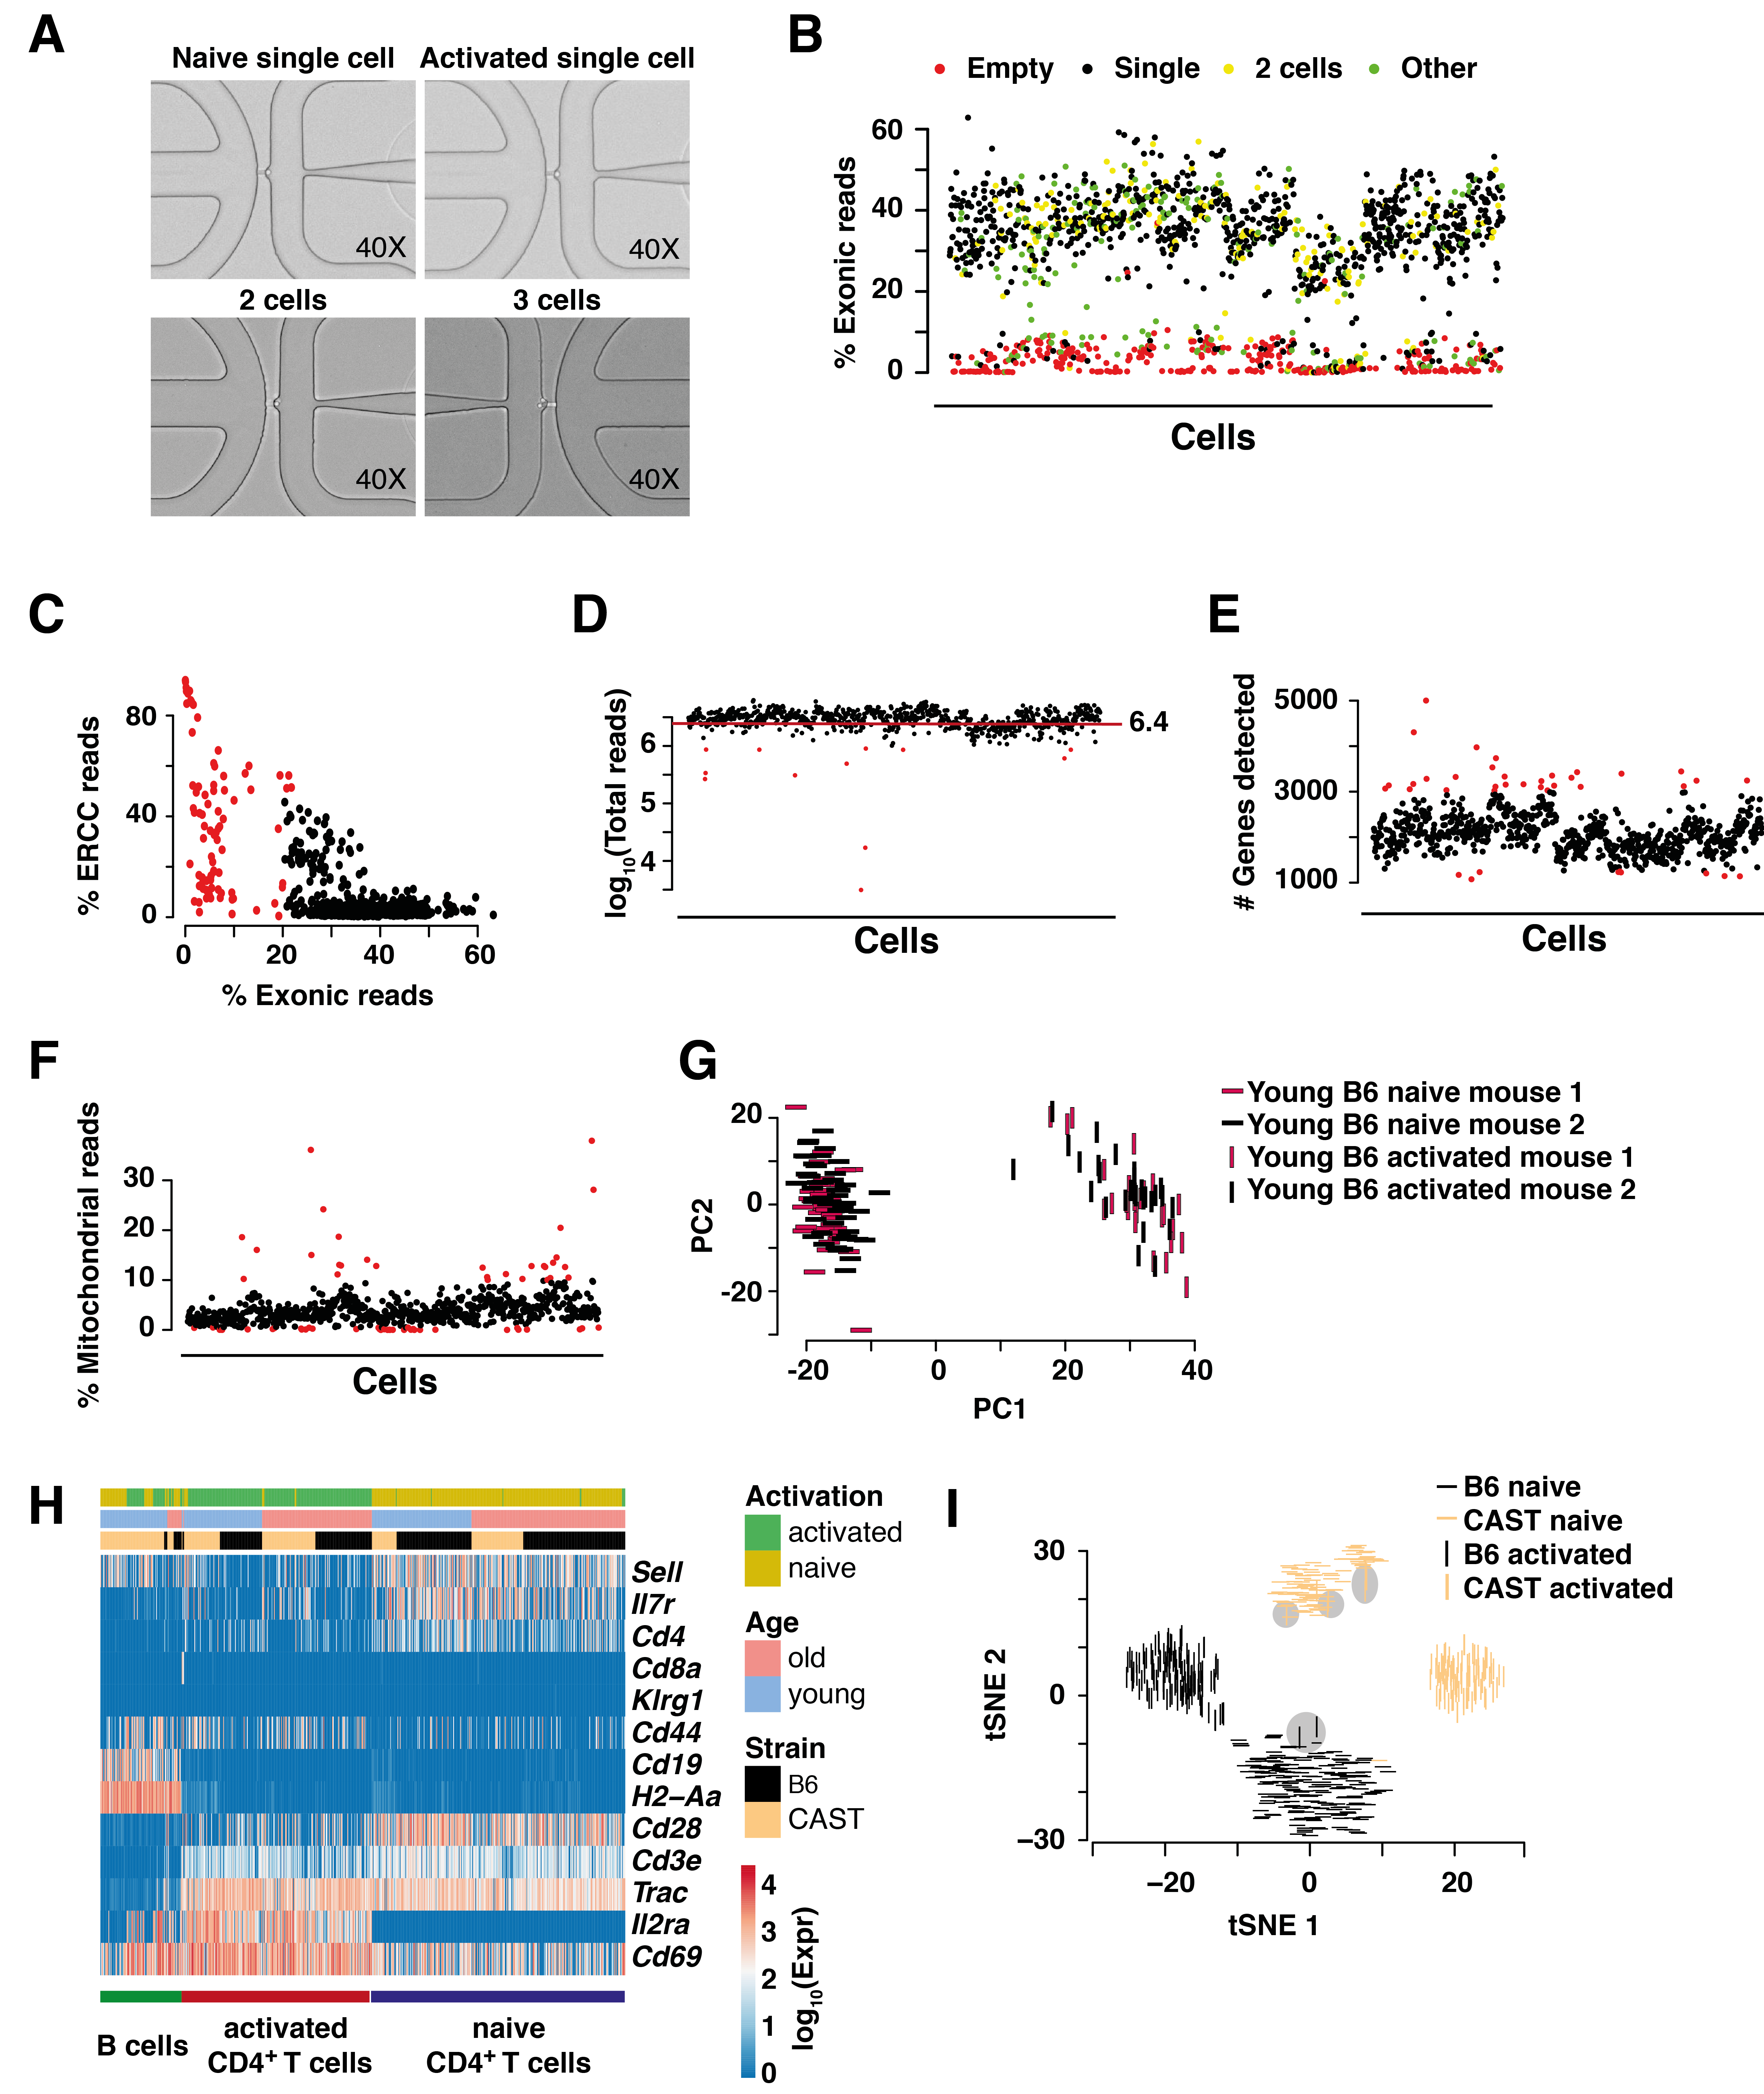
\includegraphics[width=0.9\textwidth]{Fig_3.png}
\caption[EFDR, FPR and TPR estimation using simulated data]{\textbf{EFDR, FPR and TPR estimation using simulated data (Full legend on next page).}\\
}\label{fig2:EFDR}
\end{figure}

\newpage

\captionsetup[figure]{list=no}
\addtocounter{figure}{-1}   
\captionof{figure}{\textbf{EFDR, FPR and TPR estimation using simulated data (continued).}\\
Data was simulated using the BASiCS model with model parameters set by empirical estimates based on on 98 microglia cells (see \textbf{Table \ref{tab2:datasets}}). Different samples sizes (40 - 200 cells) were simulated in replicates of 5. Differential testing was performed between 2 simulated datasets of equal size to calculate the false positive rate (FPR, number of detections divided by number of genes tested), the true positive rate (number of true positive divided by number of positives). Moreover, we report the expected false discovery rate (EFDR, \citep{Newton2004}). For each test, the EFDR was controlled to 10\% and the default minimum tolerance thresholds were used ($\tau_0 = \log_2(1.5)$, $\omega_0 = \log_2(1.5)$ and $\psi_0 = 0.41$), \textbf{(A)-(C)} Synthetic datasets generated using the null model (without changes in variability). FPR and EFDR for (A) differential mean expression, (B) differential over-dispersion and (C) differential residual over-dispersion testing using datasets with increasing samples sizes, \textbf{(D)-(E)} Synthetic datasets generated using the alternative model where 1000 genes were randomly selected and their associated over-dispersion parameters were increased or decreased by a $\log_2$ fold change of 5. TPR and EFDR for (D) differential over-dispersion testing and (E) differential residual over-dispersion testing using datasets with increasing samples sizes simulated.\\}
\captionsetup[figure]{list=yes}

As expected, the EFDR is controlled to 10\%. Furthermore, the FPR for differential mean expression and differential over-dispersion is consistently smaller than 10\% and is only slightly higher for differential residual over-dispersion testing. The TPR for differential over-dispersion and differential residual over-dispersion testing increases with increasing sample size and plateaus at 100\% \textbf{(Fig.~\ref{fig2:EFDR})}.

\subsection{Choice of hyper-parameters} \label{sec2:hyper-parameters}

As discussed above, the degrees of freedom $\eta$, the number of GRBFs  $L$ as well as their hyper-parameters ($m_l$, $h_l$) are set \emph{a priori}. Here, we explain the default values implemented in the extended BASiCS model. These were chosen to achieve a compromise between flexibility of the trend fit and the strength of shrinkage towards the estimated trend. Further discussion on the shrinkage can be found in \textbf{Section \ref{sec2:stabilization}}. \\ 

Firstly, we observed that large values of $L$ can lead to over-fitting but that small values of $L$ can limit the flexibility to capture non-linear relations between $\log(\delta_i)$ and $\log(\mu_i)$ \textbf{(Fig.~\ref{fig2:choice_hyper})}. Thus, as a parsimonious choice, we selected $L = 10$. Moreover, as in \cite{Kapourani2016}, values for $m_l$ were chosen to be equally spaced across the range of $\log(\mu_i)$:. 

\begin{equation} m_l = a + (l-1)\frac{b - a }{L-1}, \hspace{0.2cm}  l=1,\ldots, L, \end{equation} 

where $a=\min_{i\in\{1,\ldots,q_0\}}\{\log(\mu_i)\}$ and $b=\max_{i\in\{1,\ldots,q_0\}}\{\log(\mu_i)\}$. As $\mu_i$ values are unknown \emph{a priori} and change throughout the sampling procedure, $a$ and $b$ are updated every 50 MCMC iterations during the burn-in phase. Additionally, the scale hyper-parameters $h_l$ control the width of the GRBFs and, consequently, the locality of the regression. As a default, we set these as $h_l = c \times \Delta m$, where $c$ is a fixed proportionality constant and $\Delta m$ is the distance between consecutive values of $m_l$. In practice, we observed that the choice of a particular value of $c$ is not critical, as long as narrow kernels ($c<0.5$) are avoided \textbf{(Fig.~\ref{fig2:choice_hyper})}. As a default, $c = 1.2$ was chosen. \\

\begin{figure}[!h]
\centering
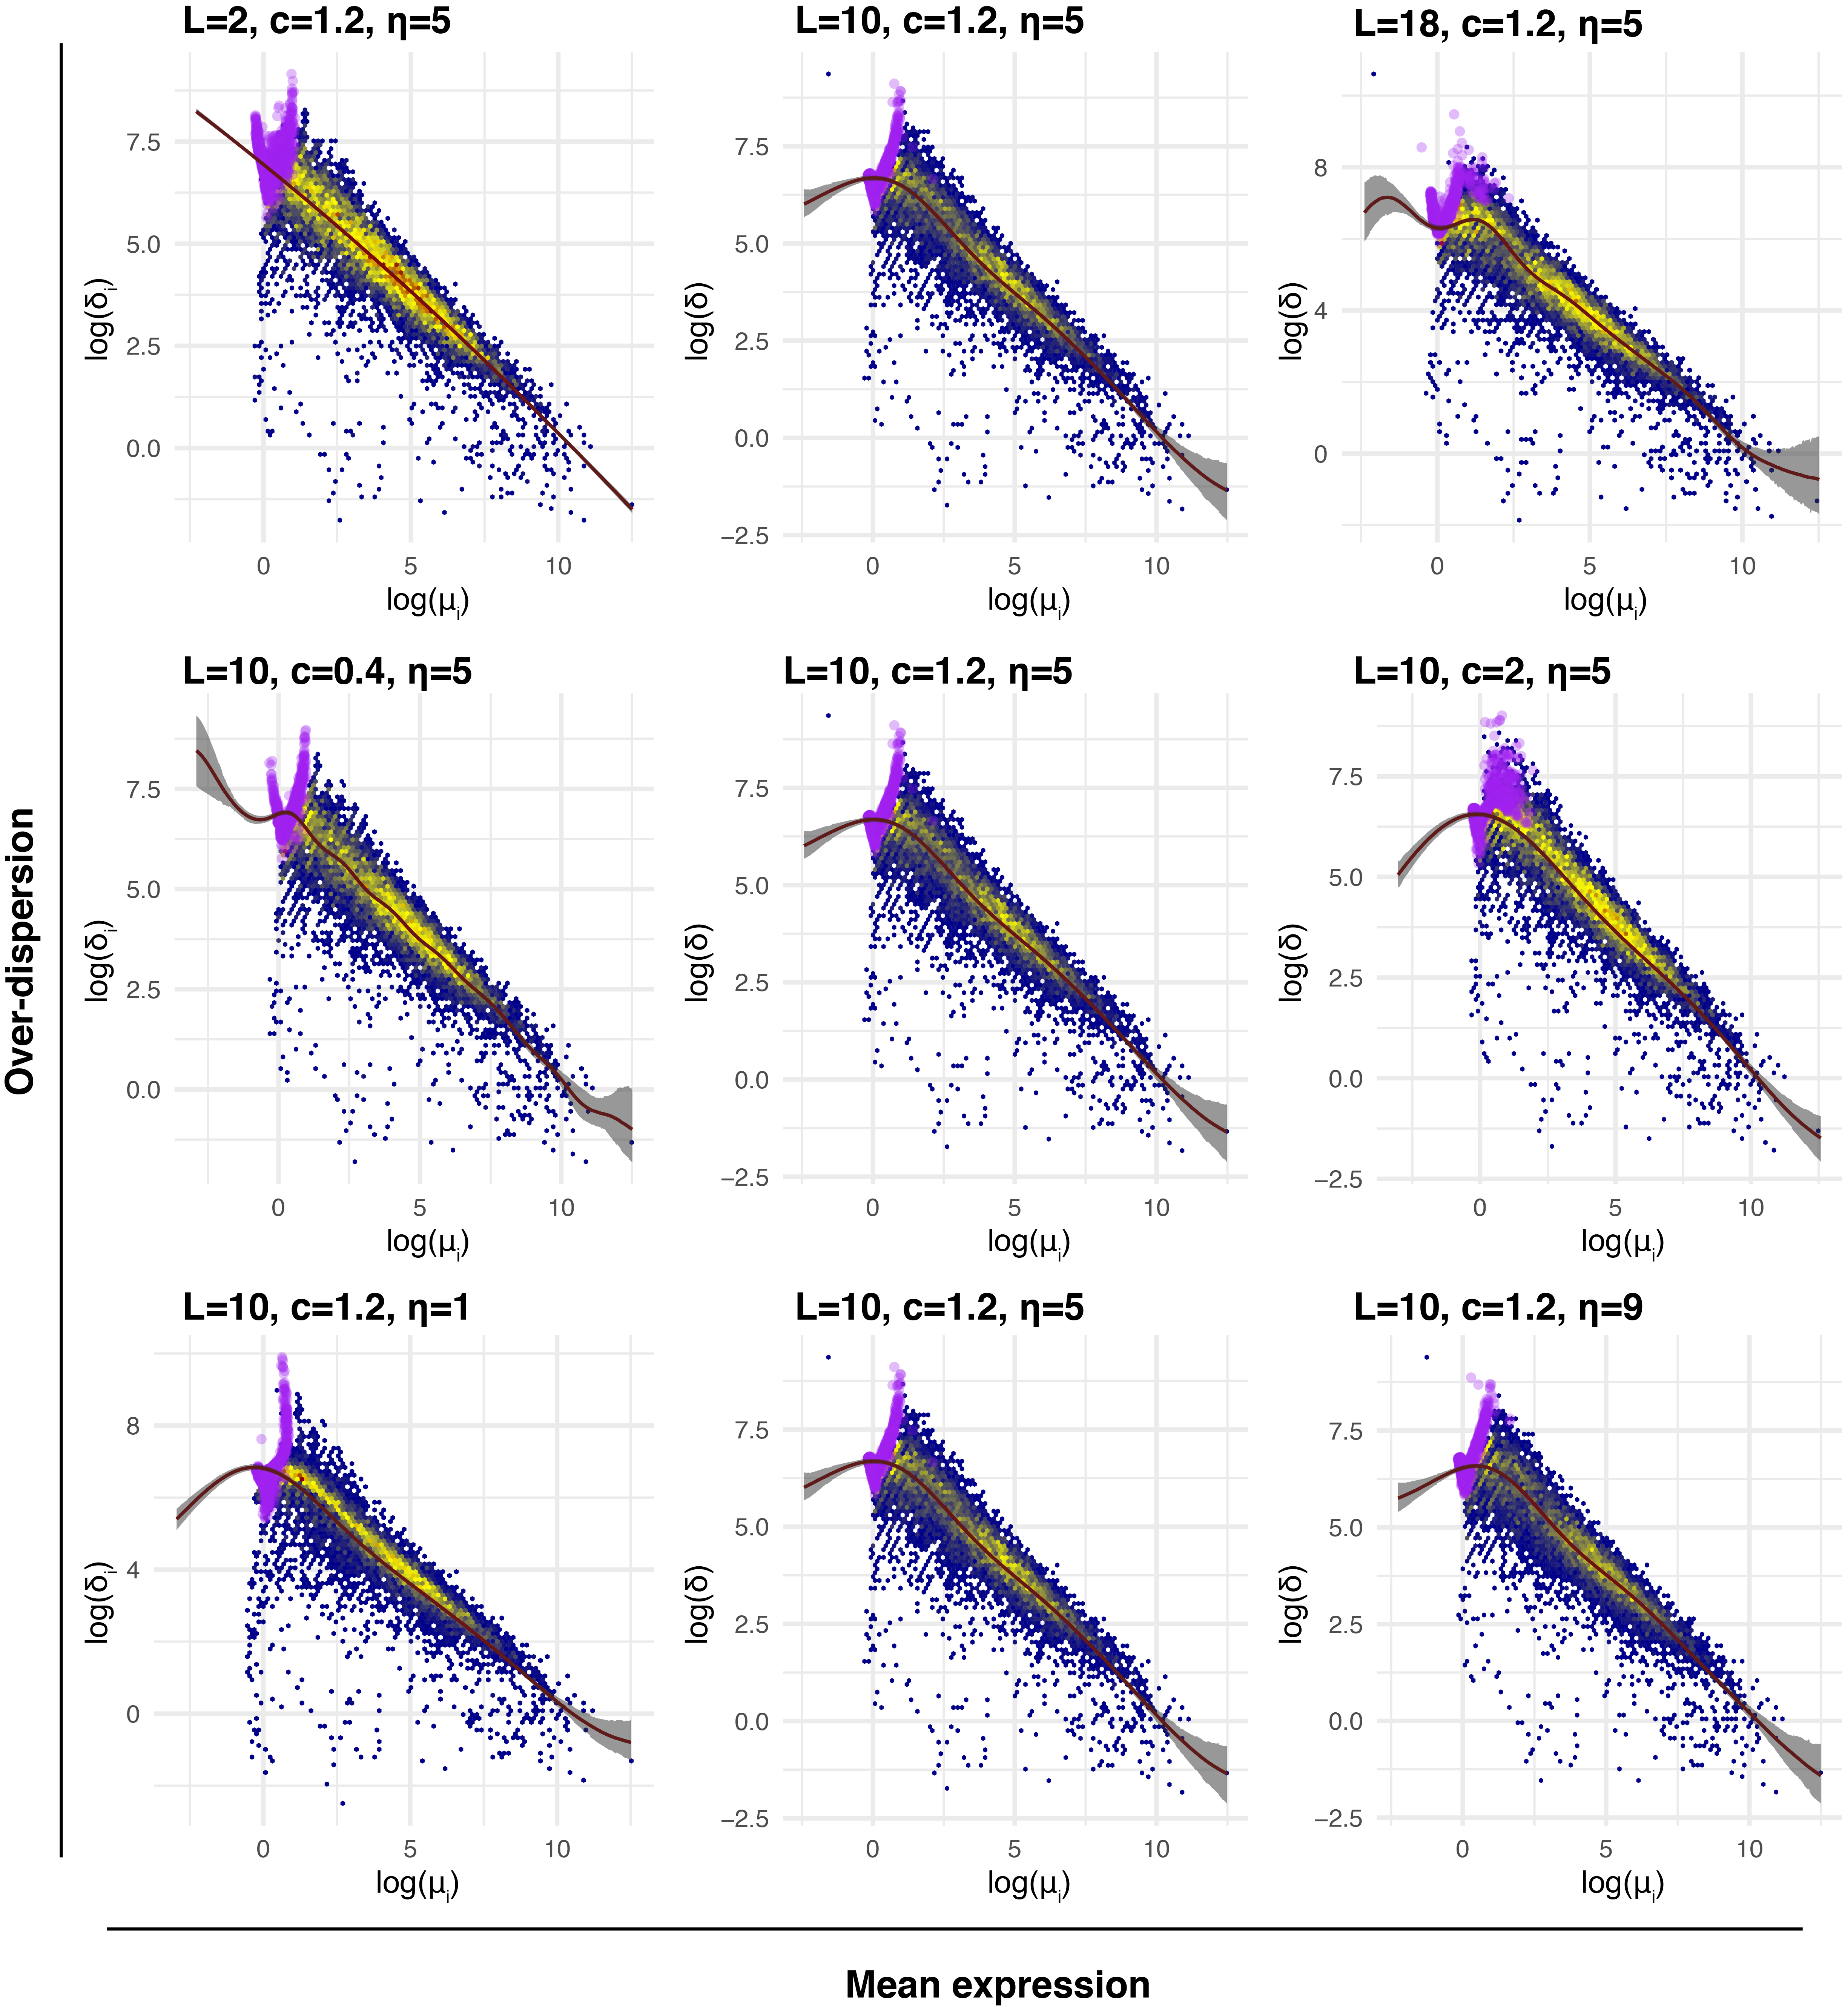
\includegraphics[width=0.8\textwidth]{Fig_4.png}
\caption[Effect of regression hyper-parameters on trend fitting]{\textbf{Effect of regression hyper-parameters on trend fitting.}\\
Posterior estimates of over-dispersion parameters $\delta_i$ are plotted versus posterior estimates of mean expression parameters $\mu_i$. The extended BASiCS model was used to estimate these parameters using naive CD4\plus{} T cells from the previous chapter. Different hyper-parameter combinations were used to fit the model. L: number of Gaussian Radial Basis Functions, c: constant to increase of decrease scale parameter, $\eta$: degrees of freedom.}
\label{fig2:choice_hyper}
\end{figure}

\newpage

The degrees of freedom $\eta$ controls the tails of the distribution for the residual term in \ref{eq::regression}. This influences the shrinkage towards the global trend and the robustness against outlying observations \textbf{(Fig.~\ref{fig2:choice_hyper})}.  If $\eta \geq 30$, $\epsilon_i$ approximately follows a normal distribution for which posterior inference for $\beta$ is known to be sensitive to outliers. Instead, small values of $\eta$ introduce heavy-tails for $\epsilon_i$, leading to more robust posterior inference. In principle, $\eta$ could be estimated within a Bayesian framework. However, this is problematic as the likelihood function associated to \ref{eq::regression} can be unbounded \citep{Fernandez1999}. Here, we opt for a pragmatic approach where the value of $\eta$ is fixed \emph{a priori}. To select a reasonable default value, we ran the regression BASiCS model for a grid of possible values of $\eta$, using the datasets described in \textbf{Table \ref{tab2:datasets}} (with $L$, $m_l$ and $h_l$ fixed as described above). In all cases, we calculated a Monte Carlo estimates for the log-likelihood associated to \ref{eq::PoissonBASiCS} as a proxy for goodness-of-fit \textbf{(Fig.~\ref{fig2:DoF}A)}. We observed that log-likelihood estimates were consistently the smallest for $\eta=1$ and that no substantial differences are observed across larger values of $\eta$. When visualizing posterior estimates for the variance $\sigma^2$ of the distribution for the residual term depending on the degrees of freedom chosen, we observe a constant increase plateauing when the distribution reaches the normal distribution at $\eta=30$ \textbf{(Fig.~\ref{fig2:DoF}B)}. We chose $\eta=5$ to be the default parameter as a compromise between shrinkage and sensitivity to outlying data points. 

\begin{figure}[!h]
\centering
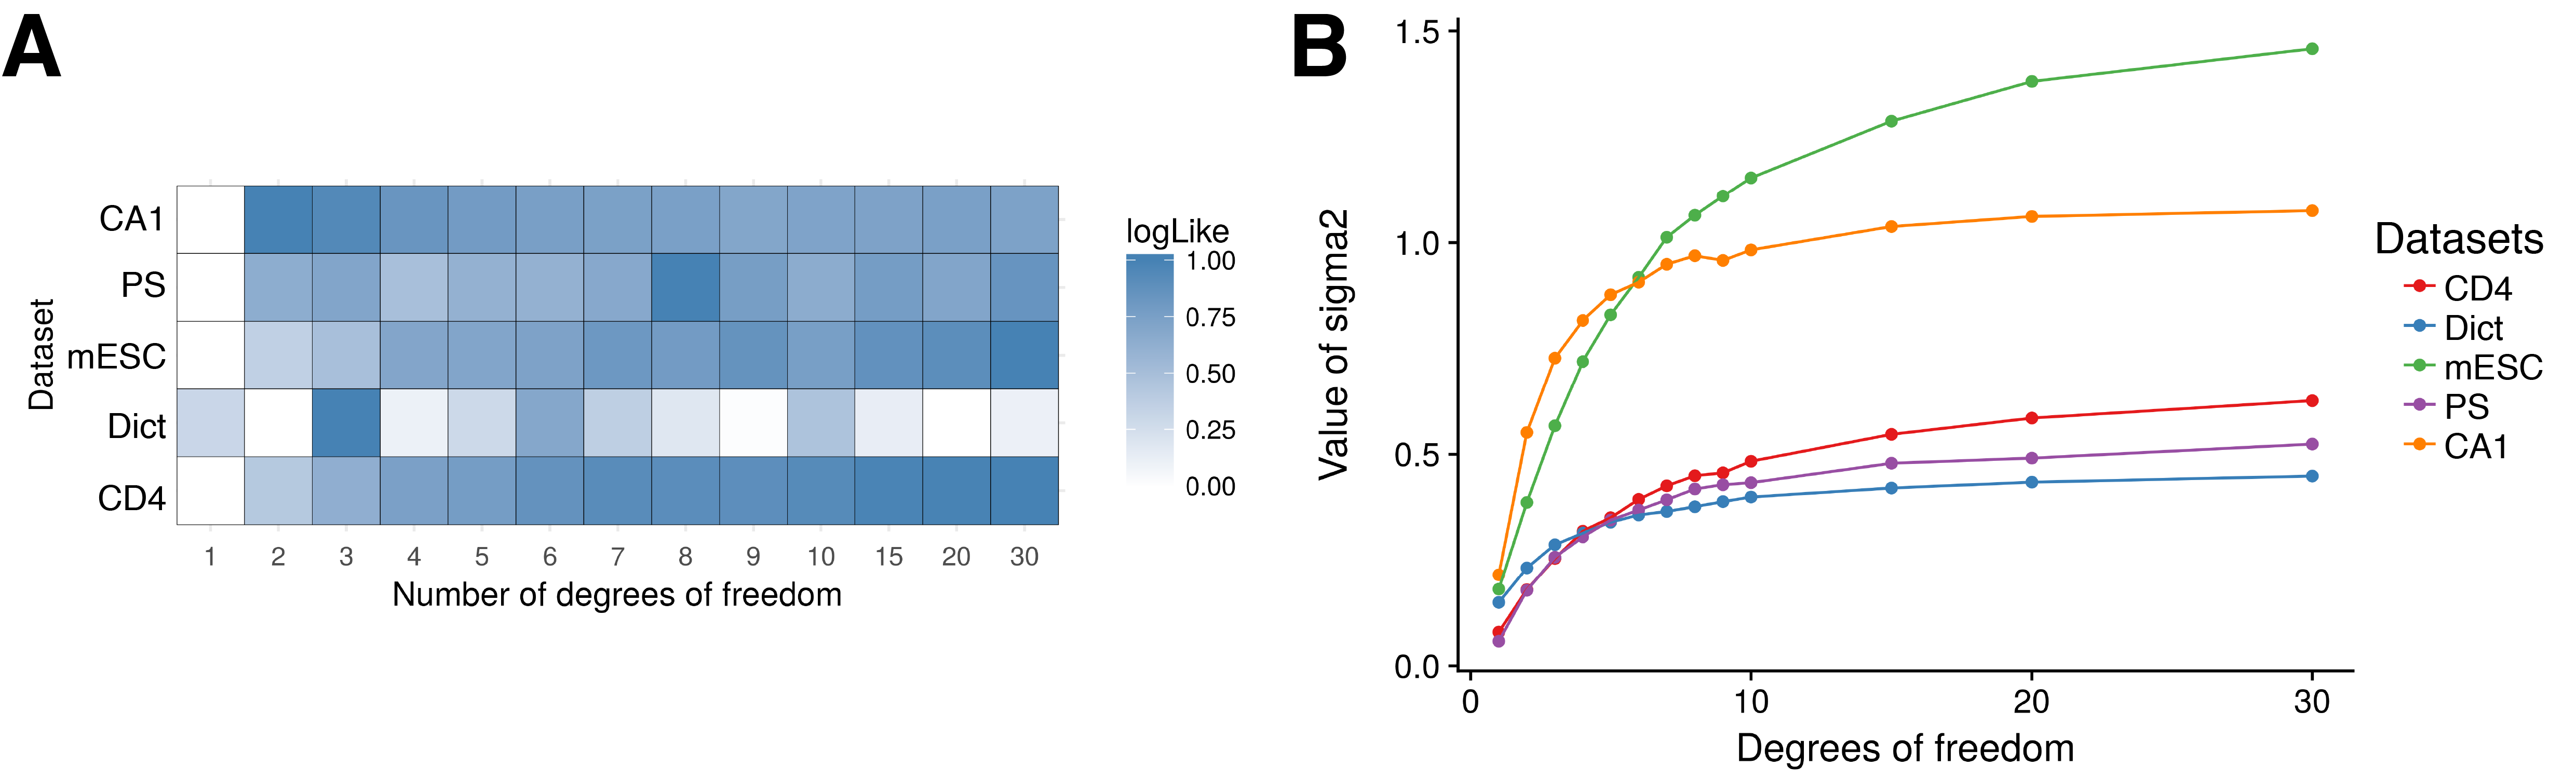
\includegraphics[width=\textwidth]{Fig_5.png}
\caption[Comparison of model fits for varying degrees of freedom]{\textbf{Comparison of model fits for varying degrees of freedom.}\\
\textbf{(A)} The regression BASiCS model was fit to datasets listed in \textbf{Table \ref{tab2:datasets}}. These include CA1 pyramidal neurons (CA1, \citep{Zeisel2015}), pool-and-split RNA 2i medium (PS, \citep{Grun2014}), mouse embryonic stem cells 2i medium (mESC, \citep{Grun2014}), Dictyostelium cells at day 0 of differentiation (Dict, \citep{Antolovic2017}) and naive CD4\plus{} T cells (CD4, \citep{Martinez-jimenez2017}). \textbf{(A)} The model was fit using varying degrees of freedom and the log-likelihood was calculated as stated in equation \ref{eq::loglik}. The log-likelihood was scaled between the highest and lowest value for each dataset. \textbf{(B)} Posterior estimates of the variance parameter $\sigma^2$ depending on the number of degrees of freedom.}
\label{fig2:DoF}
\end{figure}

Based on these observations, default values implemented in the BASiCS software are set to $L=10, c=1.2, \eta=5$. Despite this, the model's implementation also allows flexible adjustment of $L$, $c$ and $\eta$ by the user. 

\newpage

\section{Pre-processing of scRNA-Seq data used in this chapter} \label{sec2:datasets}

We employed a range of different datasets to test the proposed methodology. These datasets were selected to cover different experimental techniques (with and without unique molecular identifiers, UMI) and to encompass a variety of cell populations. Moreover, key features of each dataset can be found in \textbf{Table \ref{tab2:datasets}}. 

\subsection{Dictyostelium cells} \label{seq::data_dict}

Antolovi\'{c} \emph{et al.} studied changes in expression variability between 0 hours (undifferentiated), 3 hours and 6 hours of \emph{Dictyostelium} differentiation \cite{Antolovic2017}. Raw data is available by direct download (see Data S1 in \citep{Antolovic2017}). Across all time-points, 5 cells were removed due to low quality. Technical spike-in genes that were not detected and biological genes with an average expression (across all cells) smaller than 1 count were removed. In total, 433 cells (131 cells and 3 batches at 0h, 157 cells and 3 batches at 3h, and 145 cells and 3 batches at 6h) and 10551 genes (88 technical and 10650 biological genes) passed filtering. We used data from the 0h time point to test the functionality of our model.

\subsection{Mouse brain cells} \label{seq::data_micro}

This dataset was composed of UMI scRNA-Seq data of cells isolated from the mouse somatosensory cortex and hippocampal CA1 region \citep{Zeisel2015}. Raw data is available from Gene Expression Omnibus under accession code GSE60361. Prior to the analysis, we removed technical genes with 0 total counts and biological genes for which the average count across all 3007 cells was below 0.1. The groups comprising microglia cells and CA1 neurons were chosen to be analysed. For these groups, 98 cells (microglia), 939 cells (CA1 pyramidal neurons) and 10744 genes (10687 biological and 57 technical genes) passed filtering to be analysed.

\subsection{Pool-and-split RNAseq data} \label{seq::data_PaS}

This UMI-based dataset provides a control experiment to assess changes in biological heterogeneity in a situation where mean expression remains unchanged across conditions. Pool-and-split samples were created by pooling 1 million mESCs grown in 2i or serum medium and splitting 20pg of RNA into aliquots. These libraries are compared against single-cell samples (mESCs) \citep{Grun2014}. Raw data is available from Gene Expression Omnibus under accession code GSE54695. \\

As in \cite{Grun2014}, some cells were removed from the analysis due to low expression of the stem cell marker \textit{Oct4}. Technical genes with 0 total counts were also removed from the analysis. Additionally, lowly expressed biological genes with fewer than 0.5 counts (on average, across all samples) were excluded. This left 258 libraries (74 single mESCs grown in 2i medium, 52 single mESCs grown in serum medium, 76 pool-and-split aliquots from cells grown in 2i medium and 56 pool-and-split aliquots from cells grown in serum medium) as well as 8924 genes (50 technical spike-ins and 8874 biological genes) for the analysis. Each condition contained 2 batches.\\

Matched single molecule florescence \textit{in situ} hybridization (smFISH) data from mESCs grown in 2i and serum media were obtained from Dominic Gr\"un (Max Planck Institute of Immunobiology and Epigenetics, Freiburg, Germany) through personal communications. This smFISH experiment assayed 9 genes (\textit{Gli1}, \textit{Klf4}, \textit{Notch1}, \textit{Pcna}, \textit{Pou5f1}, \textit{Sohlh2}, \textit{Sox2}, \textit{Stag3}, \textit{Tpx2}) in more than 70 cells per condition. We excluded \textit{Notch1} from the analysis due to strong disagreement between smFISH and scRNA-Seq data of cells grown in serum medium.

\subsection{CD4\plus{} T cells} \label{seq::data_cd4}

Non-UMI scRNA-Seq data of CD4\plus{} T cells represent data analysed in  the previous chapter. Raw data is available from ArrayExpress under accession code E-MTAB-4888. To perform a variety of tests, naive and activated CD4\plus{} T cells from young \emph{Mus musculus} (B6) mice were selected. Biological genes with an average count $<~1$ and non-detected technical genes were removed from the analysis. In total, 146 cells (93 naive and 53 activated CD4\plus{} T cells) and 10553 genes (10495 biological and 58 technical genes) passed filtering. Each condition contains 2 replicates.

\subsection{CD4\plus{} T cell differentiation} \label{seq::data_cd4diff}

Non-UMI scRNA-Seq data were generated from CD4\plus{} T cells during differentiation towards T helper 1 (Th1) and T follicular helper (Tfh) cell fates after \emph{Plasmodium} infection \citep{Lonnberg2017}. Raw reads were downloaded from ArrayExpress [E-MTAB-4388] and mapped against the \emph{Mus musculus} genome (GRCm38) using \emph{gsnap} \citep{Wu2010a} with default settings. Read counting was performed using \emph{HTSeq} \citep{Anders2014} with default settings. \\

Quality control was performed by removing cells with fewer than 300,000 biological reads or fewer than 600,000 technical reads at day 2. At day 4 and 7, cells with fewer than 1,000,000 biological reads were excluded from downstream analysis. Additionally, we removed genes that did not show an average detection of more than 1 read at day 2, day 3, day 4 or day 7 after infection. After applying these criteria, 376 cells (Day 0: 16 cells, Day 2: 89, Day 3: 21, Day 4: 133, Day 7: 64, Day 7 non-infected: 53) and 7899 genes (7847 biological and 52 technical) remained for analysis. Note that, due to low sample sizes, we focused our analysis on data from day 2, day 4 and day 7 post-infection.

\begin{table}[hb	]
\centering
\caption[Datasets used for model testing and analysis]{\textbf{Datasets used for model testing and analysis.} \\
For each of the datasets analysed in this study: number of cells (2$^{nd}$ column), number of genes (biological + technical spike-ins, 3$^{rd}$ column), number of batches (4$^{th}$ column), type of data acquisition system (5$^{th}$ column), information of whether the data was generated using unique molecular identifiers (UMIs, 6$^{th}$ column) and the reference to the original study (7$^{th}$ column) are provided.}
\label{tab2:datasets}
\begin{tabular}{lllllll}
\toprule
\textbf{Dataset} & \textbf{\# cells} & \textbf{\# genes} & \textbf{\# batches} & \textbf{Protocol} & \textbf{UMIs} & \textbf{Ref.}                       \\
\midrule
Young naive  & 93       & 10553    & 2          & Fluidigm C1       & No   & \citep{Martinez-jimenez2017} \\
CD4\plus{} T cells   &        &   &          &       & No   &  \\
\midrule

Young active    & 53       & 10553    & 2          & Fluidigm C1       & No   & \citep{Martinez-jimenez2017} \\
CD4\plus{} T cells    &        &     &           &        &    &  \\
\midrule

Microglia cells                         & 98       & 10687    & 1          & Fluidigm C1       & Yes  & \citep{Zeisel2015}           \\
\midrule

CA1 pyramidal                    & 948      & 10687    & 1          & Fluidigm C1       & Yes  & \citep{Zeisel2015}           \\
neurons       &       &     &           &       &   &           \\
\midrule

Malaria infected     & 89       & 7899     & 2          & Fluidigm C1       & No   & \citep{Lonnberg2017}         \\
CD4\plus{} T cells day 2     &        &      &          &  &    &  \\
\midrule

Malaria infected  & 133      & 7899     & 2          & Fluidigm C1       & No   & \citep{Lonnberg2017}         \\
CD4\plus{} T cells day 4     &       &      &    &  &    &\\
\midrule

Malaria infected  & 64       & 7899     & 1          & Fluidigm C1       & No   & \citep{Lonnberg2017}         \\
CD4\plus{}  T cells day 7    &   & &  &  &  &   \\
\midrule

Dictyostelium             & 131      & 10738    & 3          & Fluidigm C1       & No   & \citep{Antolovic2017}        \\
cells day 0  &  &   &   &  & & \\
\midrule

Pool-split RNA                 & 76       & 8924     & 2          & CEL-Seq           & Yes  & \citep{Grun2014}            \\
2i medium  &  &  & &  &  & \\
\midrule

mESC 2i medium    & 74       & 8924     & 2          & CEL-Seq           & Yes  & \citep{Grun2014} \\
\midrule

Pool-split RNA             & 56       & 8924     & 2          & CEL-Seq           & Yes  & \citep{Grun2014}            \\
serum medium &  &      &         &   &   &  \\
\midrule

mECS serum medium & 52       & 8924     & 2          & CEL-Seq           & Yes  & \citep{Grun2014} \\
\bottomrule       
\end{tabular}
\end{table}


\section{The informative prior stabilizes parameter estimation}
\label{sec2:stabilization}

Our joint prior formulation has introduced a non-linear regression to capture the overall trend between gene-specific over-dispersion parameters $\delta_i$ and mean expression parameters $\mu_i$. Thus, we also refer to the extended model induced by this prior as the \textit{regression} BASiCS model. Accordingly, the model induced by the original independent prior specification \citep{Vallejos2016} is referred to as the \textit{non-regression} BASiCS model.\\ 

\subsection{Dataset specificity of the regression trend and the shrinkage}

To study the performance of the regression BASiCS model, we applied it to a variety of scRNA-Seq datasets. Each dataset is unique in its composition, covering a range of different cell types and experimental protocols (see \textbf{Section \ref{sec2:datasets}} and \textbf{Table \ref{tab2:datasets}}). Qualitatively, we observe that the inferred regression trend varies substantially across different datasets \textbf{(Fig.~\ref{fig2:datasets}}, justifying the choice of a flexible semi-parametric approach (see \textbf{Section \ref{sec2:extended_BASiCS}} and \textbf{Section \ref{sec2:hyper-parameters}}). Moreover, as expected, we observe that residual over-dispersion parameters $\epsilon_i$ are not confounded by mean expression. Additionally, we assessed whether the residual over-dispersion parameter is biased by the percentage of zero counts per gene. This feature increases for lowly expressed genes due to technical expression drop-outs. Nevertheless, posterior estimates of gene-specific residual over-dispersion parameters are not confounded by the percentage of zero counts per gene \textbf{(Fig.~\ref{fig2:datasets}}. \\

Next, we observed that the regression BASiCS model shrinks the posterior estimates for $\mu_i$ and $\delta_i$ towards the regression trend. This is due to the joint prior specification on $(\mu_i,\delta_i)'$ and in line with the shrinkage observed in Love \emph{et al.} \citep{Love2014}. The strength of this shrinkage is dataset-specific, being more prominent in sparser datasets with a higher frequency of zero counts \textbf{(Fig.~\ref{fig2:datasets}A)} and for lowly-expressed genes where measurement error is greatest. 

\newpage

\begin{figure}[!h]
\centering
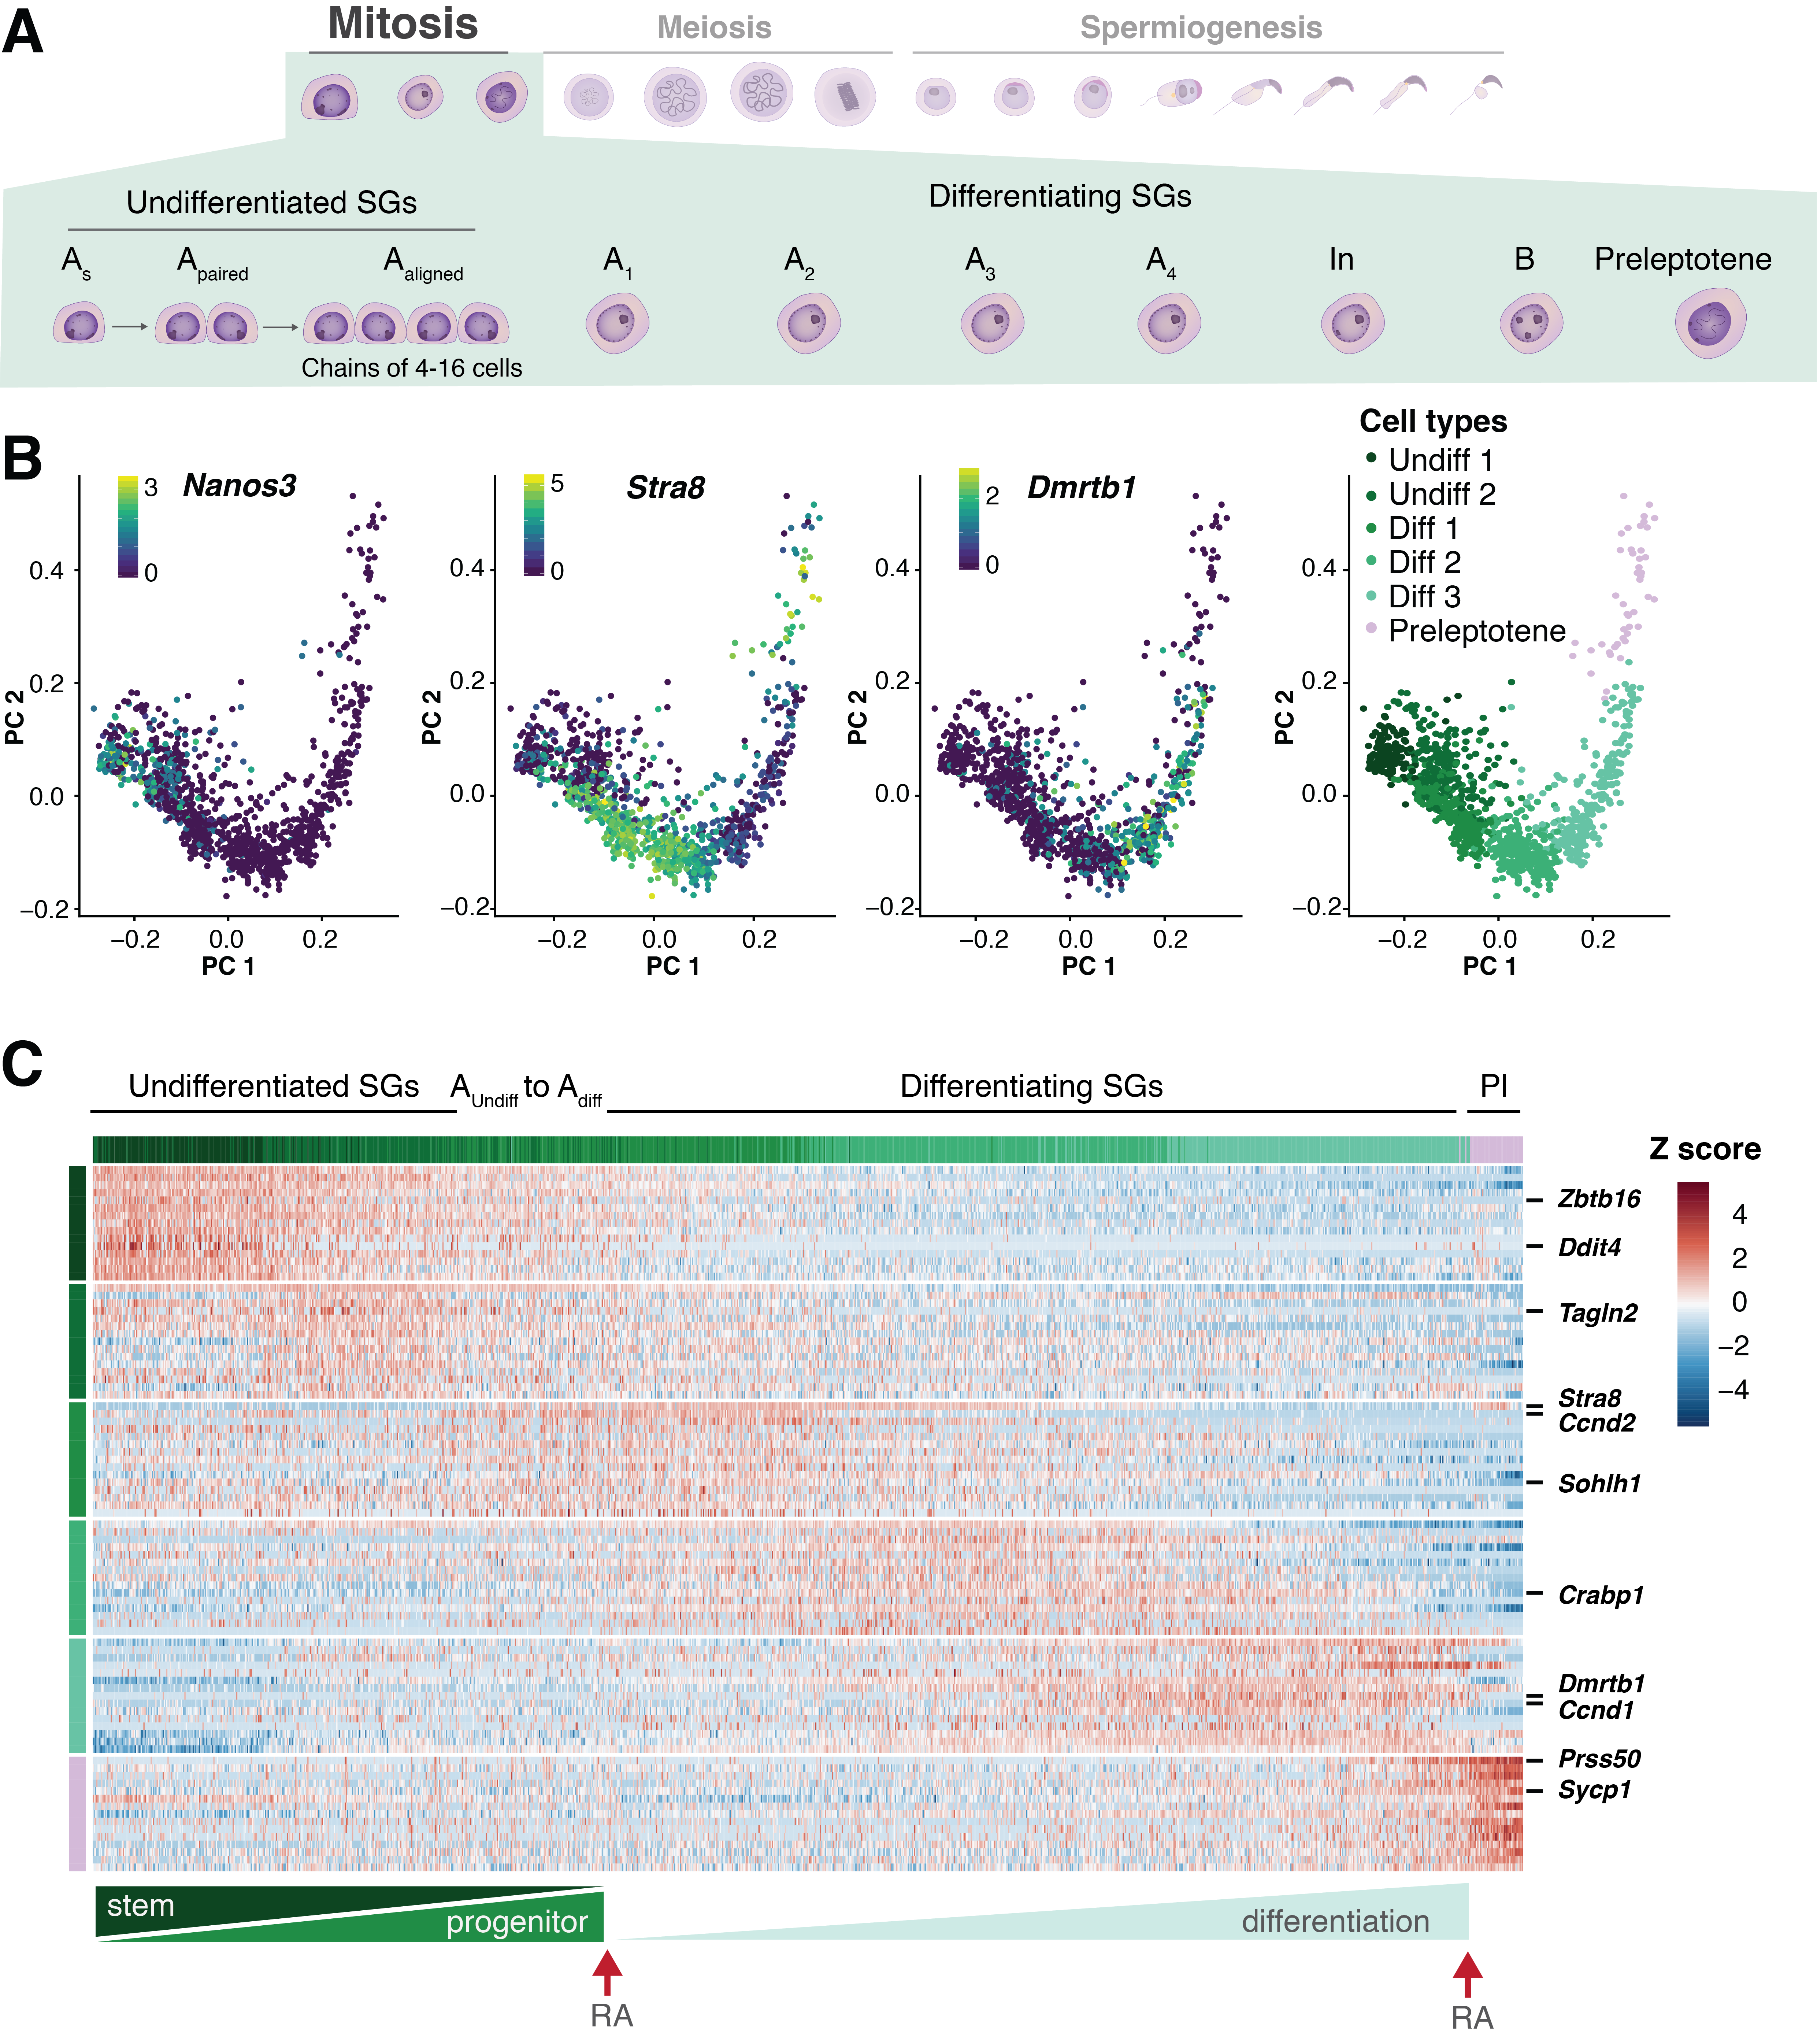
\includegraphics[width=0.95\textwidth]{Fig_6.png}
\caption[Parameter estimation using a variety of scRNA-Seq datasets]{\textbf{Parameter estimation using a variety of scRNA-Seq datasets.}\\
Model parameters were estimated using the regression and non-regression BASiCS models on \textbf{(A)} naive CD4\plus{} T cells \citep{Martinez-jimenez2017}, \textbf{(B)} \textit{Dictyostelium} cells prior to differentiation (day 0) \citep{Antolovic2017}, \textbf{(C)} microglia cells \citep{Zeisel2015} and \textbf{(D)} pool-and-split RNA \citep{Grun2014}. These datasets were selected to highlight situations with different levels of sparsity (i.e.~the proportion of zero counts, see fourth column). The colour code within the scatterplots is used to represent areas with high (yellow/red) and low (blue) density of genes. \textbf{First column:} gene-specific over-dispersion $\delta_i$ versus mean expression $\mu_i$ as estimated by the non-regression BASiCS model.\textbf{Second column:} gene-specific over-dispersion $\delta_i$ versus mean expression $\mu_i$ as estimated by the regression BASiCS model. The red line indicates the estimated regression trend. Purple dots indicate genes detected (i.e.~with at least one count) in less than 2 cells. \textbf{Third column:} gene-specific residual over-dispersion $\epsilon_i$ versus mean expression $\mu_i$ as estimated by the regression BASiCS model. \textbf{Forth column:} gene-specific posterior estimates for residual over-dispersion $\epsilon_i$ parameters versus percentage of zero counts for each gene.\\}
\label{fig2:datasets}
\end{figure}

\newpage

\subsection{Stabilization of posterior inference}

Subsequently, we asked whether or not the shrinkage introduced by the regression BASiCS model improves posterior inference. To assess this, we compared estimates for gene-specific parameters across: (i) different sample sizes and (ii) different gene expression levels. Both, the sample size and the level of expression influence posterior estimation of model parameters due to loss of power when few cells are used to estimate parameters for lowly expressed genes. More concretely, we used a large dataset containing 939 CA1 pyramidal neurons \citep{Zeisel2015} to artificially generate smaller datasets by randomly sub-sampling 50-500 cells. For each sample size, parameter estimates were then obtained using both the regression and non-regression BASiCS models. 
Based on parameter estimates using the non-regression model, we split the genes into three sets: lowly expressed ($\mu_i<1.89$), medium expressed ($1.89<\mu_i<5.37$) and highly expressed ($\mu_i>5.37$). These cut-off values were chosen such that roughly a third of genes classifies into each category. The distribution of these estimates is summarised in \textbf{Fig.~\ref{fig2:parameter_stabilization}}. \\

\begin{figure}[!h]
\centering
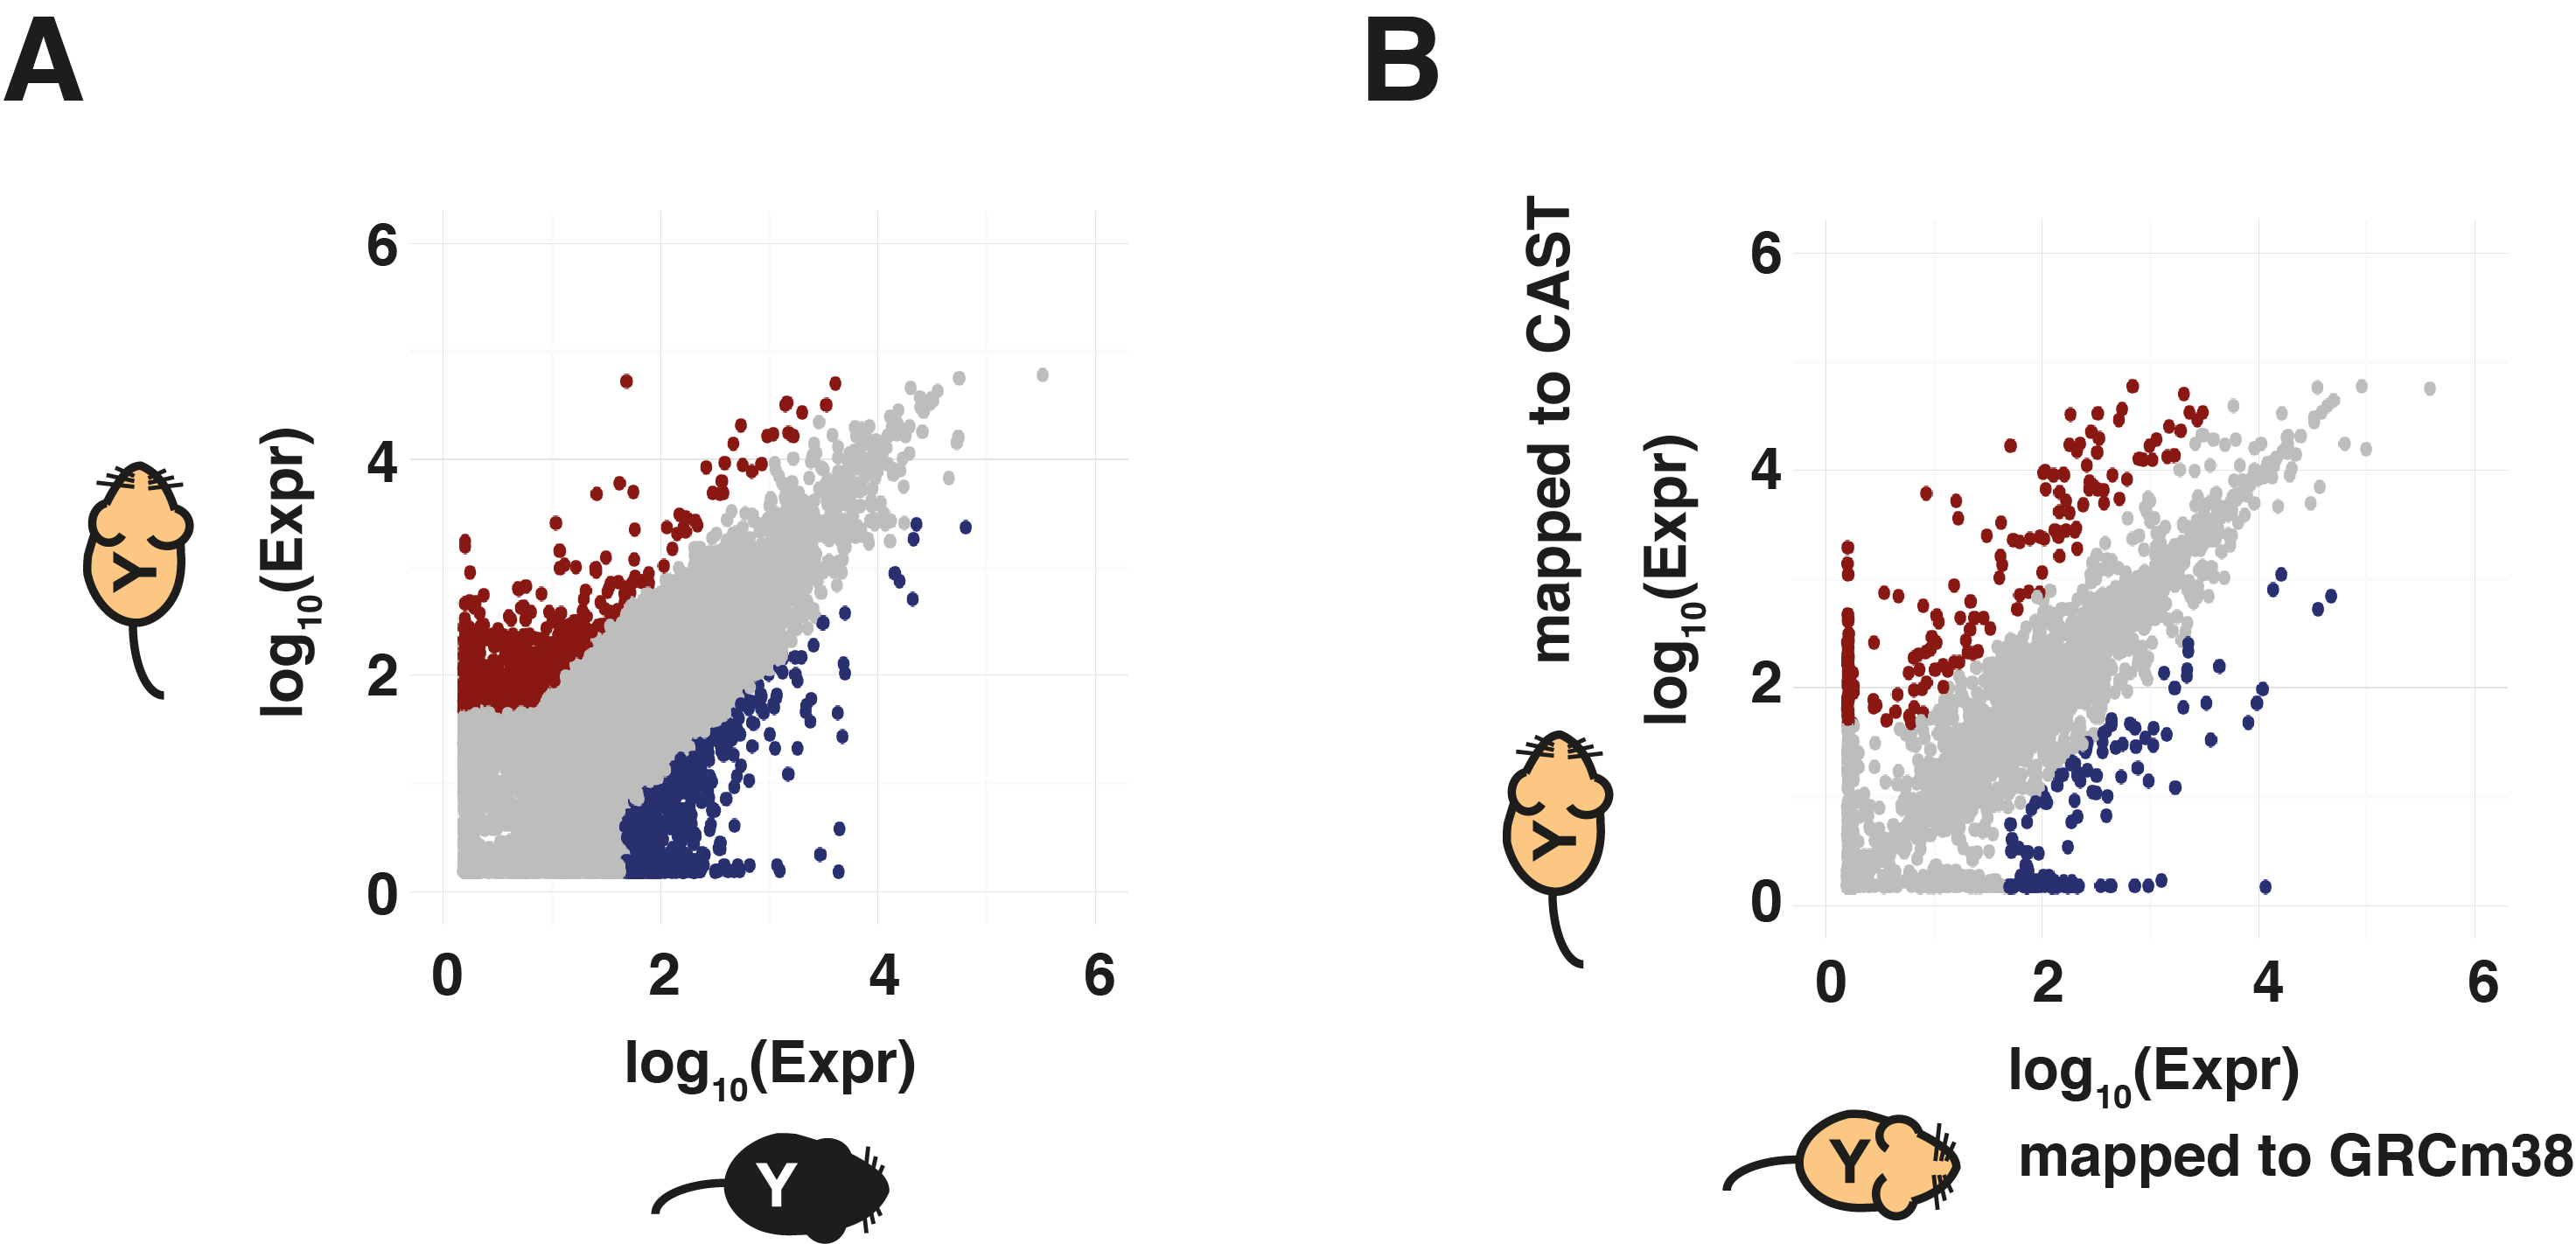
\includegraphics[width=\textwidth]{Fig_7.png}
\caption[Estimation of gene-specific model parameters for varying sample sizes]{\textbf{Estimation of gene-specific model parameters for varying sample sizes.}\\
The regression (orange) and non-regression (blue) BASiCS models were used to estimate gene-specific model parameters for lowly (lower panels), medium (mid panels) and highly (upper panels) expressed genes across populations with varying numbers of cells. These were generated by randomly sub-sampling cells from a population of 939 CA1 pyramidal neurons \citep{Zeisel2015}. Extended results based on multiple downsampling experiments are displayed in \textbf{Fig.~\ref{fig2:parameter_stabilization2}}. \textbf{(A-C)} For a single sub-sampling experiment, boxplots summarize the distribution of gene-specific estimates for (A) mean expression parameters $\mu_i$ (log-scale), (B) over-dispersion parameters $\delta_i$ (log-scale) and (C) residual over-dispersion parameters $\epsilon_i$.}
\label{fig2:parameter_stabilization}
\end{figure}

Firstly, we observe that both the regression and non-regression BASiCS models led to comparable and largely stable mean expression estimates $\mu_i$ across different sample sizes and expression levels \textbf{(Fig.~\ref{fig2:parameter_stabilization}A)}. Secondly, in line with the results in \textbf{Fig.~\ref{fig2:datasets}}, the main differences between the methods arise when estimating the over-dispersion parameters $\delta_i$ \textbf{(Fig.~\ref{fig2:parameter_stabilization}B )}. In particular, we observe that the non-regression BASiCS model appears to underestimate $\delta_i$ for lowly expressed genes when the sample size is small (with respect to the parameter estimates obtained based on the full dataset of 939 cells). This is due to the original, non-informative prior: $\delta_i\sim\textnormal{log-N}(0,a_\delta^2)$. In the case of lowly expressed genes, the data is not informative and the over-dispersion parameters are estimated as $\delta_i\approx{}0$. In contrast, the shrinkage introduced by our regression BASiCS model aids parameter estimation, leading to robust estimates even for the smallest sample size. This is particularly important for rare cell populations where large sample sizes are difficult to obtain. A similar effect is observed for genes with medium and high expression levels, where the non-regression BASiCS model appears to overestimate $\delta_i$. We also observe that estimates of residual over-dispersion parameters $\epsilon_i$ are stable across sample sizes and expression levels. \textbf{Fig.~\ref{fig2:parameter_stabilization2}A-C} summarizes 10 replicates of the down-sampling experiment performed in \textbf{Fig.~\ref{fig2:parameter_stabilization}A-C}. For each sub-sampling experiment, sample size and gene set, we computed the median $\log_2$ fold change in $\mu_i$ and $\delta_i$ and the median difference for $\epsilon_i$ between estimates and the \emph{pseudo} ground truth. The median and the range of these values across 10 sub-sampling experiment is used for visualization purposes \textbf{(Fig.~\ref{fig2:parameter_stabilization2}D-F)}. 

\subsection{Validation of gene-specific posterior estimates by smFISH}

As an external validation, we compared our posterior estimates of gene-specific model parameters obtained from scRNA-Seq data to empirical estimates from matched single-molecule fluorescence \textit{in situ} hybridization (smFISH) data of mouse embryonic stem cells grown in 2i and serum media \citep{Grun2014}. Firstly, posterior estimates of mean-expression parameters $\mu_i$ exhibit high correlation to smFISH mean transcript counts \textbf{(Fig.~\ref{fig2:parameter_stabilization2}D)}. Secondly, we also observe a strong correlation between posterior estimates for over-dispersion parameters $\delta_i$ and the empirical CV$^2$ values obtained from smFISH data \textbf{(Fig.\ref{fig2:parameter_stabilization2}E)}. Finally, a similar behaviour is observed when comparing posterior estimates of residual over-dispersion parameters $\epsilon_i$ to a residual CV$^2$ \textbf{(Fig.\ref{fig2:parameter_stabilization2}F)}. As in \cite{Brennecke2013}, to obtain residual CV$^2$ values for the smFISH data, we fitted a gamma generalized linear model with identity link (\textit{glmgam.fit} of the \textit{statmod} package in R) between the CV$^2$ and the reciprocal log-transformed mean transcript counts.

\newpage

\begin{figure}[!h]
\centering
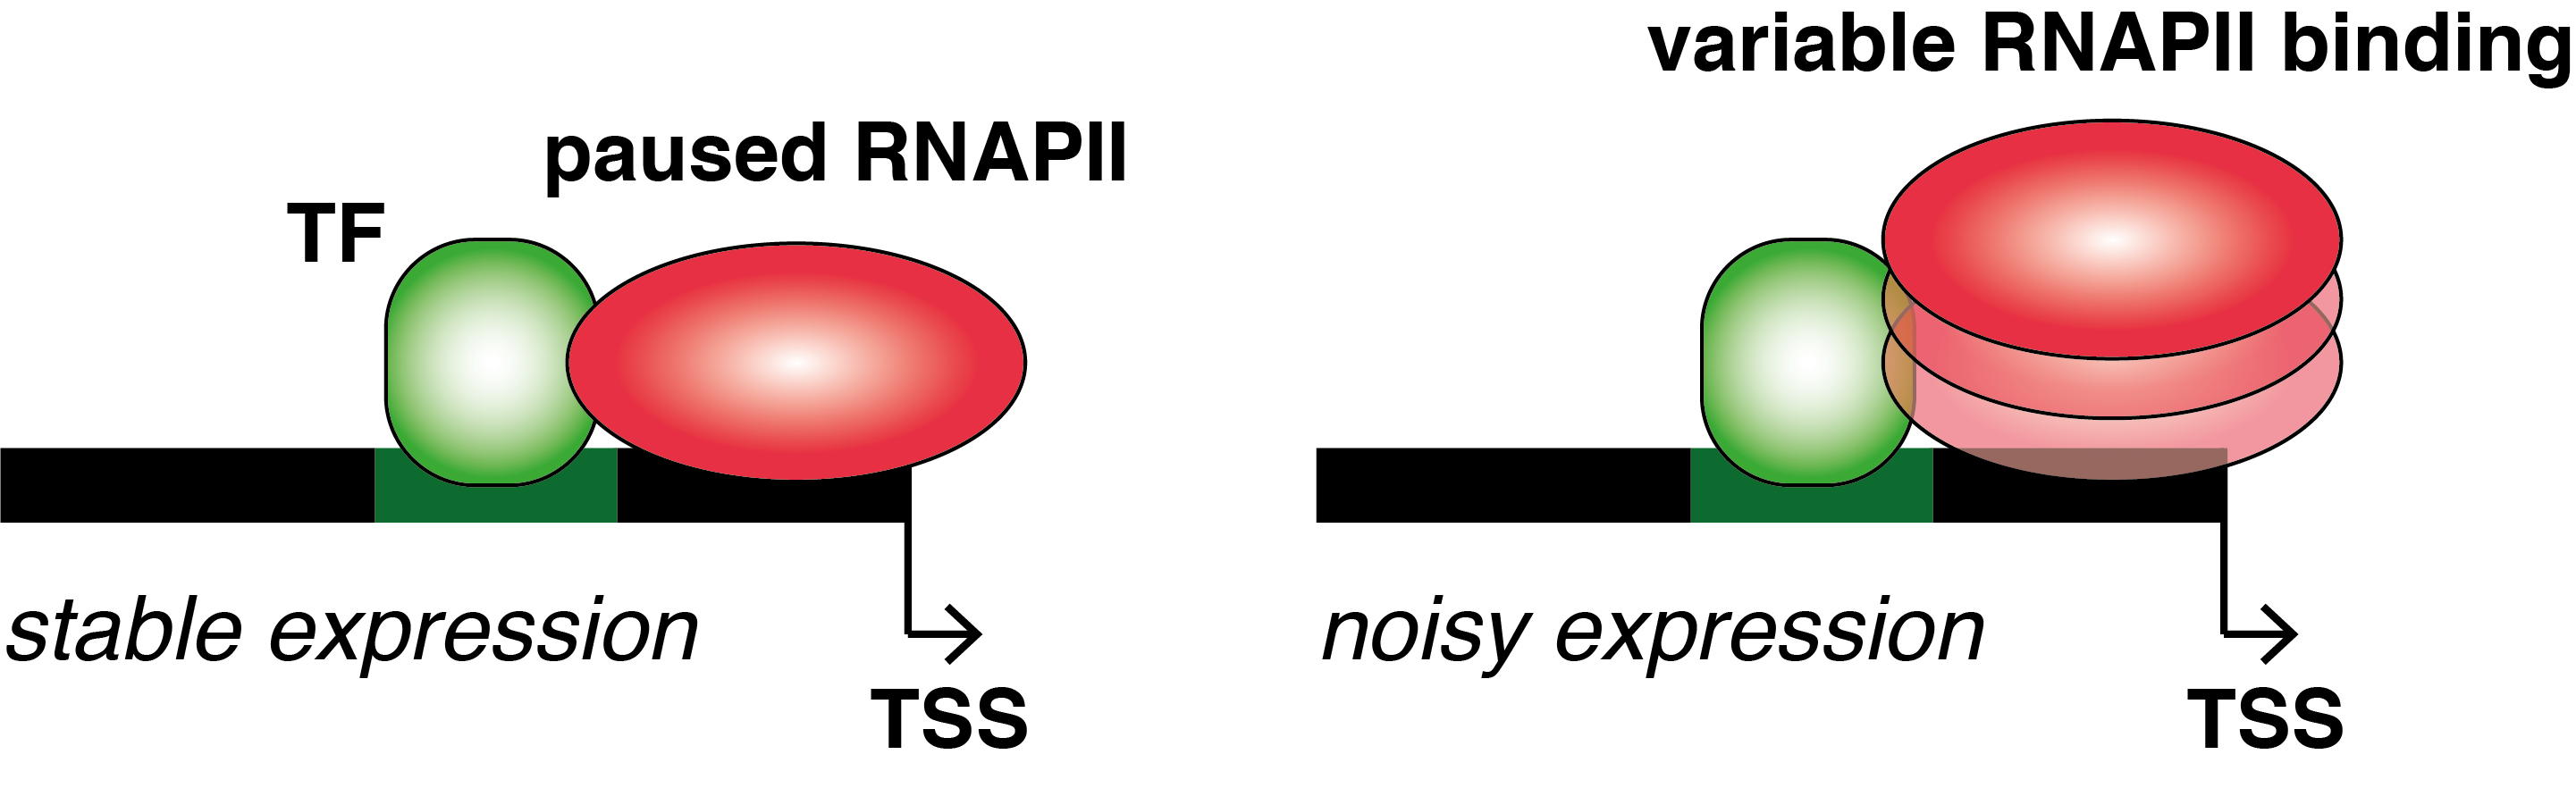
\includegraphics[width=0.9\textwidth]{Fig_8.png}
\caption[Stability of posterior estimates for gene-specific parameters]{\textbf{Stability of posterior estimates for gene-specific parameters.}\\
\textbf{(A-C)} The regression (orange) and non-regression (blue) BASiCS models were used to estimate gene-specific model parameters for lowly (lower panels), medium (mid panels) and highly (upper panels) expressed genes across populations with varying numbers of cells. These were generated by randomly sub-sampling cells from a population of 939 pyramidal CA1 neurons \citep{Zeisel2015} similar to \textbf{Fig.~\ref{fig2:parameter_stabilization}}. For 10 sub-sampling experiments, parameter estimates were compared against a \textit{pseudo} ground truth (pgt). The latter is defined as the parameter estimates obtained for the full population of 939 cells using the regression BASiCS model. For each sub-sampling experiment, gene-specific log$_2$ fold changes ($\log_2(\mu_i/\mu_{i,pgt})$ and $\log_2(\delta_i/\delta_{i,pgt})$) and distances ($\epsilon_i - \epsilon_{i,pgt}$) between the estimates and the pgt were computed. For visualisation purposes, the medians across genes for each sub-sampling experiment are presented. \textbf{(D-F)} Matched scRNA-Seq and smFISH data measured on mouse embryonic stem cells grown in 2i and serum media \citep{Grun2014} was used to validate the performance of the regression BASiCS model. Gene-specific parameter estimates obtained by the regression BASiCS model were compared against empirical estimates calculated based on smFISH data. This comparison includes 8 genes, measured in both conditions. Pearson's correlation is indicated for each comparison. \textbf{(G)} Estimates of mean expression parameters $\mu_i$ (log-scale) are plotted against mean transcript count (smFISH). \textbf{(H)} Estimates of over-dispersion parameters $\delta_i$ (log-scale) are plotted against the squared coefficient of variation (CV$^2$) of transcript counts (smFISH). \textbf{(I)} Estimates for residual over-dispersion parameters $\epsilon_i$ are compared against residual estimates of variability estimated for the smFISH data.}
\label{fig2:parameter_stabilization2}
\end{figure}

\newpage

\section{Expression variability during immune responses}

Here, we illustrate how the regression BASiCS model assesses changes in expression variability using CD4\plus{} T cell activation and differentiation. For all datasets, pre-processing steps are described in \textbf{Section \ref{sec2:datasets}}. 

\subsection{Testing variability changes upon immune activation}

As described in the previous chapter, the non-regression BASiCS model only allows assessing changes in variability for genes that remain stable in gene expression across conditions. Here, we extend the analysis done on the previous chapter and test for changes in variability in parallel to changed in mean expression. \\

To identify gene expression changes during early T cell activation, we compared CD4\plus{} T cells before (naive) and after (active) 3 hours of stimulation (see \textbf{Section \ref{sec1:activation}} and \citep{Martinez-jimenez2017}). For both conditions, we ran the regression BASiCS model independently and performed differential mean expression and differential variability testing using the residual over-dispersion parameters. Testing changes in variability through residual over-dispersion allows testing across all genes, including the large set of genes that are up-regulated upon immune activation \textbf{(Fig.~\ref{fig1:immune_activation})}. The latter include immune-response genes and critical drivers for CD4\plus{} T cell functionality that had to be excluded from analysis in the previous chapter.

\subsubsection{Comparison between the regression and non-regression BASiCS model}

Firstly, we compare the results obtained by the regression BASiCS model to those presented in \textbf{Section \ref{sec1:activation}}.  
To allow a direct comparison of the results, the same inclusion criteria as in the previous chapter is adopted, i.e.~we excluded genes with low mean expression ($\mu_i<50$) in both conditions from testing. Moreover, the minimum tolerance thresholds were also adapted to match the choices in \textbf{Section \ref{sec1:activation}}. To detect differentially expressed genes (mean) a minimum tolerance threshold $\tau_0 = 2$ was used \textbf{(Fig.~\ref{fig2:model_comparison}A)}. To compare the detection of differentially over-dispersed genes, we performed differential mean expression testing using a stringent minimum tolerance threshold $\tau_0 = 0$ for both models (this is to avoid the results to be confounded by changes in mean, see upper panel in \textbf{Fig.~\ref{fig2:model_comparison}B}). For the 463 genes that are detected as non-differentially expressed by both models for this threshold, a total of 111 genes are detected as differentially over-dispersed by either model (minimum tolerance log$_2$ fold change threshold $\omega_0 = \log_2(1.5) = 0.58$). Out of this set, 93 genes ($\sim$83\%) are detected as differentially over-dispersed by both models (see lower panel in \textbf{Fig.~\ref{fig2:model_comparison}B}).

\newpage

\begin{figure}[!h]
\centering
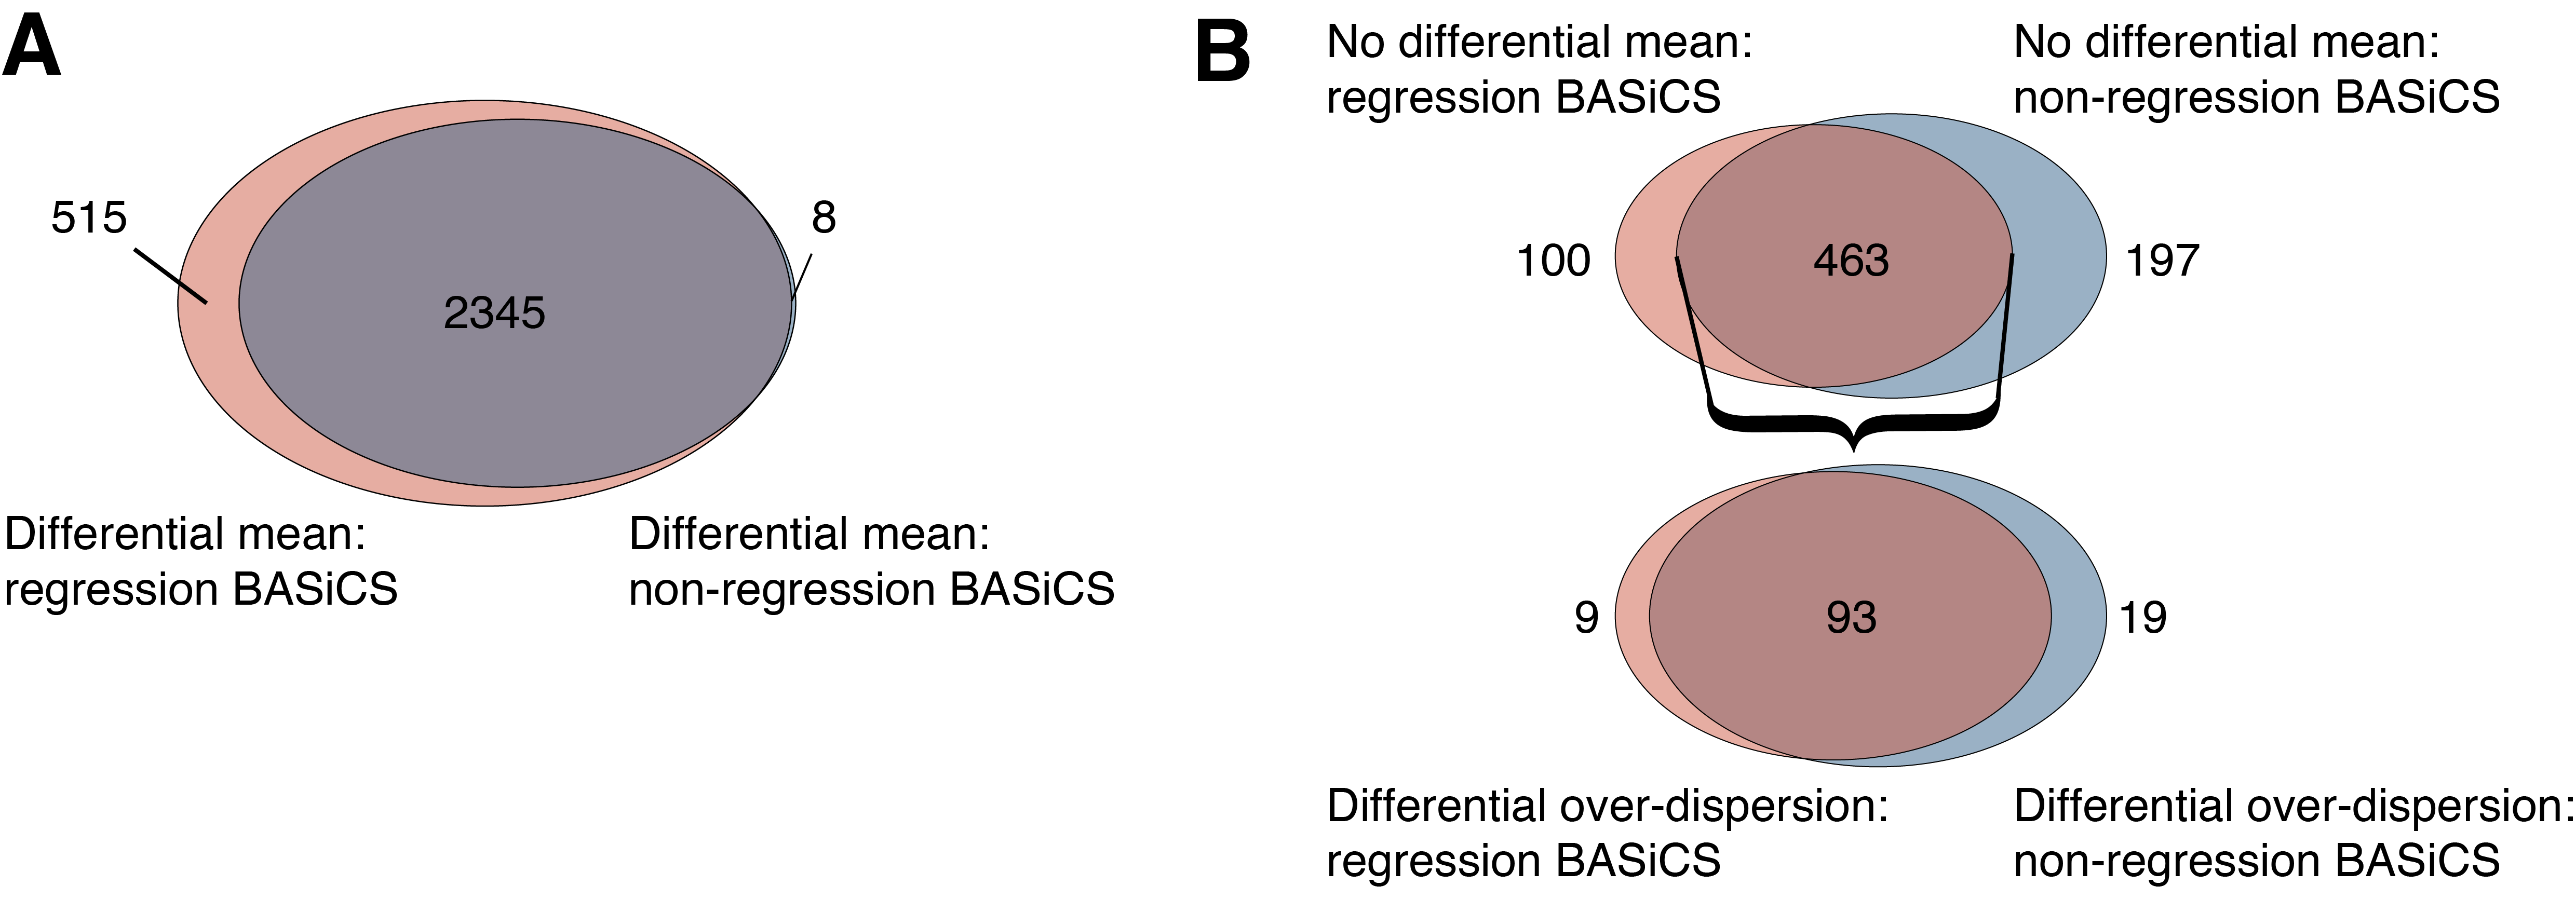
\includegraphics[width=\textwidth]{Fig_9.png}
\caption[Differential testing comparison between the regression and non-regression BASiCS model]{\textbf{Differential testing comparison between the regression and non-regression BASiCS model.}\\
(A)-(B) Results of differential testing between naive and activated CD4\plus{} T cells were compared between the regression and non-regression BASiCS models. As in \textbf{Section \ref{sec1:activation}}, genes with low mean expression ($\mu_i<50$) in both conditions were excluded from testing. \textbf{(A)} Overlap of differentially expressed genes (mean) using a minimum tolerance threshold $
\tau_0=2$ obtained by the regression and non-regression BASiCS models (EFDR = 10\%),\textbf{(B)} Upper panel: overlap of genes detected as non-differentially expressed using an stringent minimum tolerance threshold $\tau_0=0$ obtained by the regression and non-regression BASiCS models (EFDR = 10\%). Lower panel: overlap of differentially over-dispersed genes using a minimum tolerance threshold $\omega_0=\log_2(1.5)$ obtained using the regression and non-regression  BASiCS models for the 463 genes detected as non-differentially expressed by both models (EFDR = 10\%).\\}
\label{fig2:model_comparison}
\end{figure}

\subsubsection{Differential testing during immune activation}

In this chapter, we exclude genes whose estimated mean expression parameter $\mu_i$ was below 1 from the differential testing. Furthermore, a $\log_2$ fold change threshold $\tau_0 = 1$ was adopted for mean expression testing. Unlike the more stringent threshold used in the previous chapter ($\tau_0 = 2$), this choice allows us to detect more subtle changes in mean expression. Moreover, the default threshold $\psi_0 = 0.41$ was used for differential variability testing. The expected false discovery rate (EFDR) was controlled to 10\%. By using these thresholds, our model classifies genes into four categories based on their expression dynamics: down-regulated upon activation with (i) lower and (ii) higher variability, and up-regulated with (iii) lower and (iv) higher variability \textbf{(Fig.~\ref{fig2:immune_activation}A)}. \\

Genes with up-regulated expression upon activation and decreased expression variability encode components of the splicing machinery (e.g.~\textit{Sf3a3}, \textit{Plrg1}), RNA polymerase subunits (e.g.~\textit{Polr2l}, \textit{Polr1d}) as well as translation machinery components (e.g.~\textit{Ncl}, \textit{Naf1}) (see \textbf{Fig.~\ref{fig2:immune_activation}B}). These biosynthetic processes help naive T cells to rapidly enter a program of proliferation and effector molecule synthesis \citep{Tan2017,Araki2017}. Therefore, rapid, uniform up-regulation of these transcripts would assist such processes. This observation also confirms previous findings that the translational machinery is tightly regulated during early immune activation (see \textbf{Section \ref{sec1:activation}}).

\begin{figure}[!h]
\centering
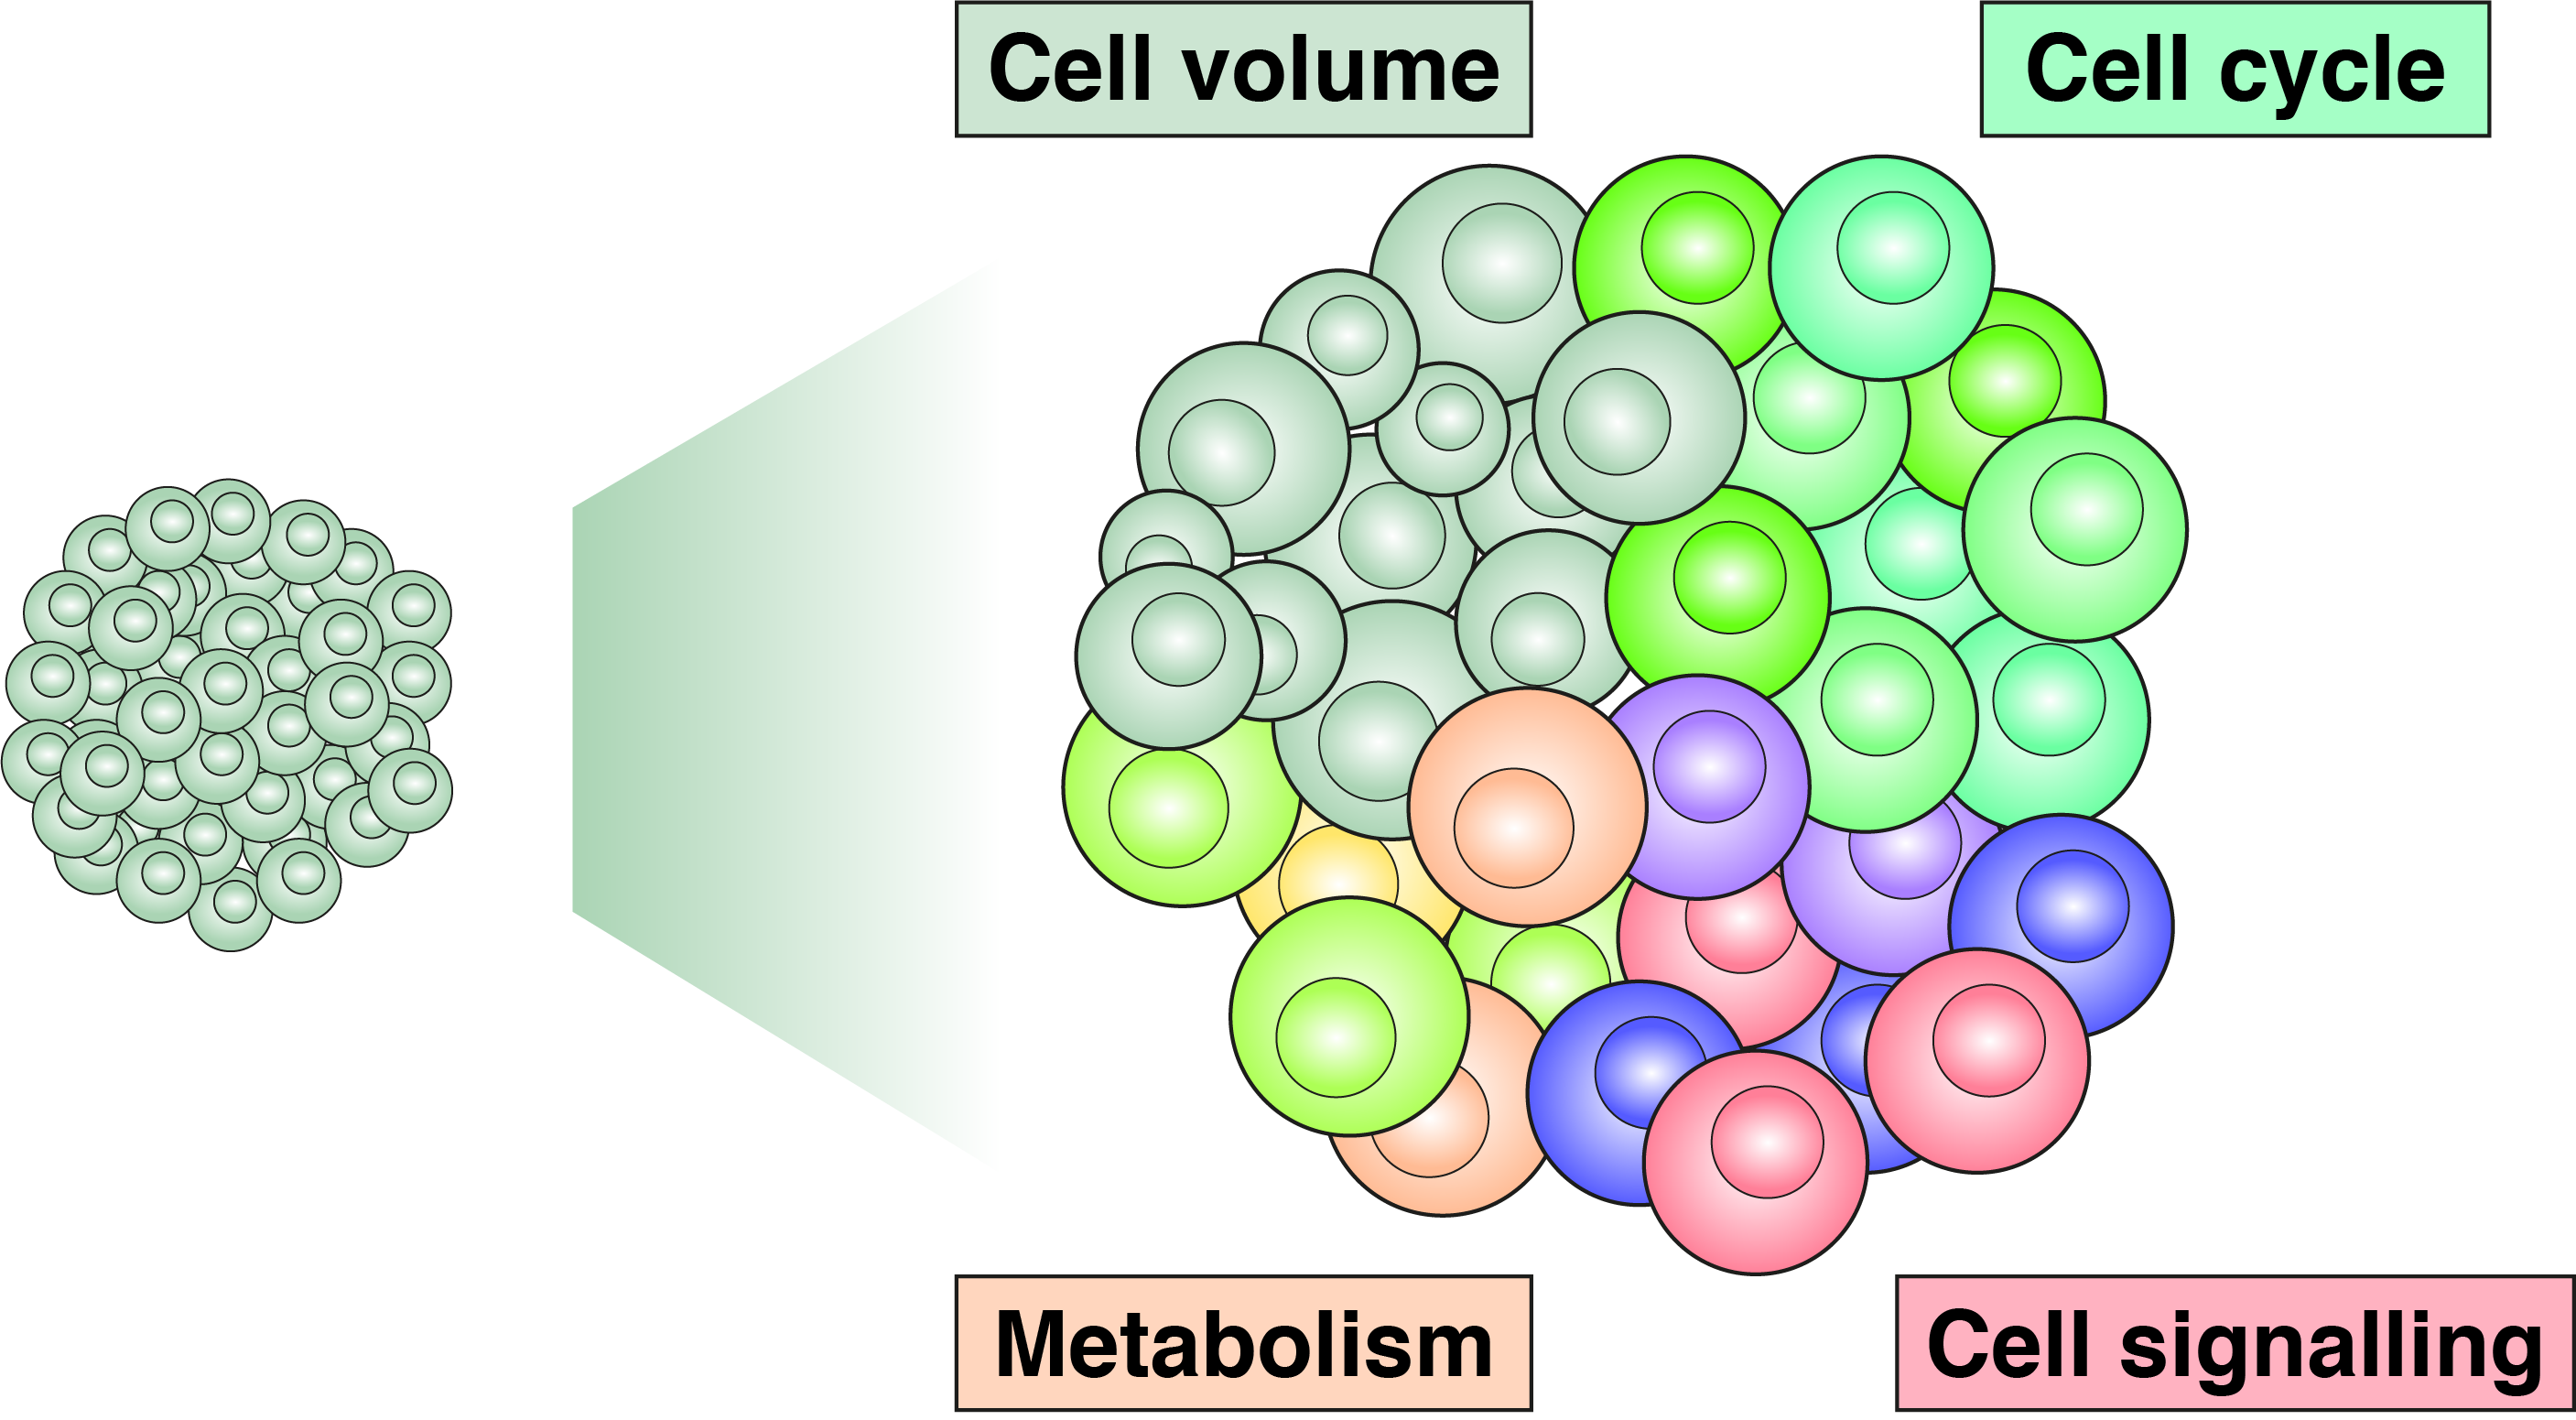
\includegraphics[width=0.7\textwidth]{Fig_10.png}
\caption[Changes in expression patterns during early immune activation]{\textbf{Changes in expression patterns during early immune activation.}\\
Differential testing (mean and residual over-dispersion) was performed between naive and activated murine CD4\plus{} T cells taken from the previous chapter. This analysis uses a minimum tolerance threshold of $\tau_0=1$ for changes in mean expression and a minimum tolerance threshold of $\psi_0=0.41$ for differential residual over-dispersion testing (expected false discovery rate is fixed at 10\%). \textbf{(A)} For each gene, the difference in residual over-dispersion estimates (Active - Naive) is plotted versus the log$_2$ fold change in mean expression (Active/Naive). Genes with statistically significant changes in mean expression and variability are coloured based on their regulation (up/down-regulated, higher/lower variability), \textbf{(B-C)} Denoised expression counts across the naive (purple) and active (green) CD4\plus{} T cell population are visualized for representative genes that (B) increase in mean expression and decrease in expression variability and (C) increase in mean expression as well as expression variability  upon immune activation. Each dot represents a single cell.}
\label{fig2:immune_activation}
\end{figure}

\newpage

In contrast, genes with up-regulated expression and increased expression variability (see \textbf{Fig.~\ref{fig2:immune_activation}C}) include the death-inducing and inhibitory transmembrane ligands Fas ligand (\textit{Fasl}) and PD-L1 (\textit{Cd274}), the regulatory transcription factor Smad3 (\textit{Smad3}), and the TCR-induced transcription factor, Oct2 (\textit{Pou2f2}). Additionally, we detect a heterogeneous up-regulation in the mRNA expression of the autocrine/paracrine growth factor IL-2 (\textit{Il2}) upon immune activation. This is in line with previous reports of binary IL-2 expression within a population of activated T cells, which has been suggested to be necessary for a scalable antigen response \citep{Fuhrmann2016}. Heterogeneity in expression of these genes suggests that, despite their uniform up-regulation of biosynthetic machinery, the T cells in this early activation culture represent a mixed population with varying degrees of activation and/or regulatory potential. \\

For each of these gene sets, functional annotation analysis was performed using all tested genes as background. The functional annotation clustering tool in DAVID \citep{Dennis2003} was used to cluster annotation categories based on similarity and sort them according to their enrichment score. Here, we list the top 3 functional annotation clusters per gene set and their corresponding enrichment score (ES):
\begin{itemize}
\item \textbf{Down-regulated with lower variability:} Pleckstrin homology domain (ES = 1.57), G protein signalling (ES = 1.51), glycosidase (ES = 1.49),
\item \textbf{Down-regulated with higher variability:} Ankyrin repeat-containing domain (ES = 2.19), GTPase mediated signalling (ES = 1.51), steroid biosynthesis (ES = 0.89), 
\item \textbf{Up-regulated with lower variability:} RNA polymerase (ES = 1.6), RNA binding (ES = 1.53), splicing (ES = 1.41),
\item \textbf{Up-regulated with higher variability:} Cytokine-cytokine receptor interaction (ES = 1.65), WD40 repeat (ES = 1.22), transcription (ES = 1.18).
\end{itemize}

\subsubsection{Effect of expression outliers on changes in variability}

We observe that for some genes (e.g.~\textit{Plrg1}), changes in variability are driven by a small number of outlier cells with high expression. The interpretation of these results is not trivial as it could reflect very subtle sub-structure or genuine changes in variability. To explore this, we performed the following synthetic experiment: We artificially created a mixed population of cells by combining 5 activated CD4\plus{} T cells with a population of 93 naive CD4\plus{} T cells therefore simulating expression outliers. Subsequently, we performed a differential testing (mean and residual over-dispersion) between this mixed population and a \textit{pure} population of 93 naive CD4\plus{} T cells. As expected, this analysis shows an overall increase in variability in the mixed population. For example, among the genes that exhibit higher mean expression and higher residual over-dispersion in the mixed population, we found \textit{Il2} which is up-regulated upon CD4\plus{} T cell activation \textbf{(Fig.~\ref{fig2:mixture_population}A)}. Moreover, we observe that the genes in this category are enriched for those that are only expressed in the 5 activated CD4\plus{} T cells \textbf{(Fig.~\ref{fig2:mixture_population}B)}. This result suggests that differential variability testing can potentially uncover markers for heterogeneous cell states or cell types which can provide important biological insights. However, changes in residual over-dispersion that are driven by outliers can also reflect unwanted contamination (e.g.~mixed cell types), hence careful data filtering and clustering analysis should be performed prior to differential variability testing. 

\begin{figure}[!h]
\centering
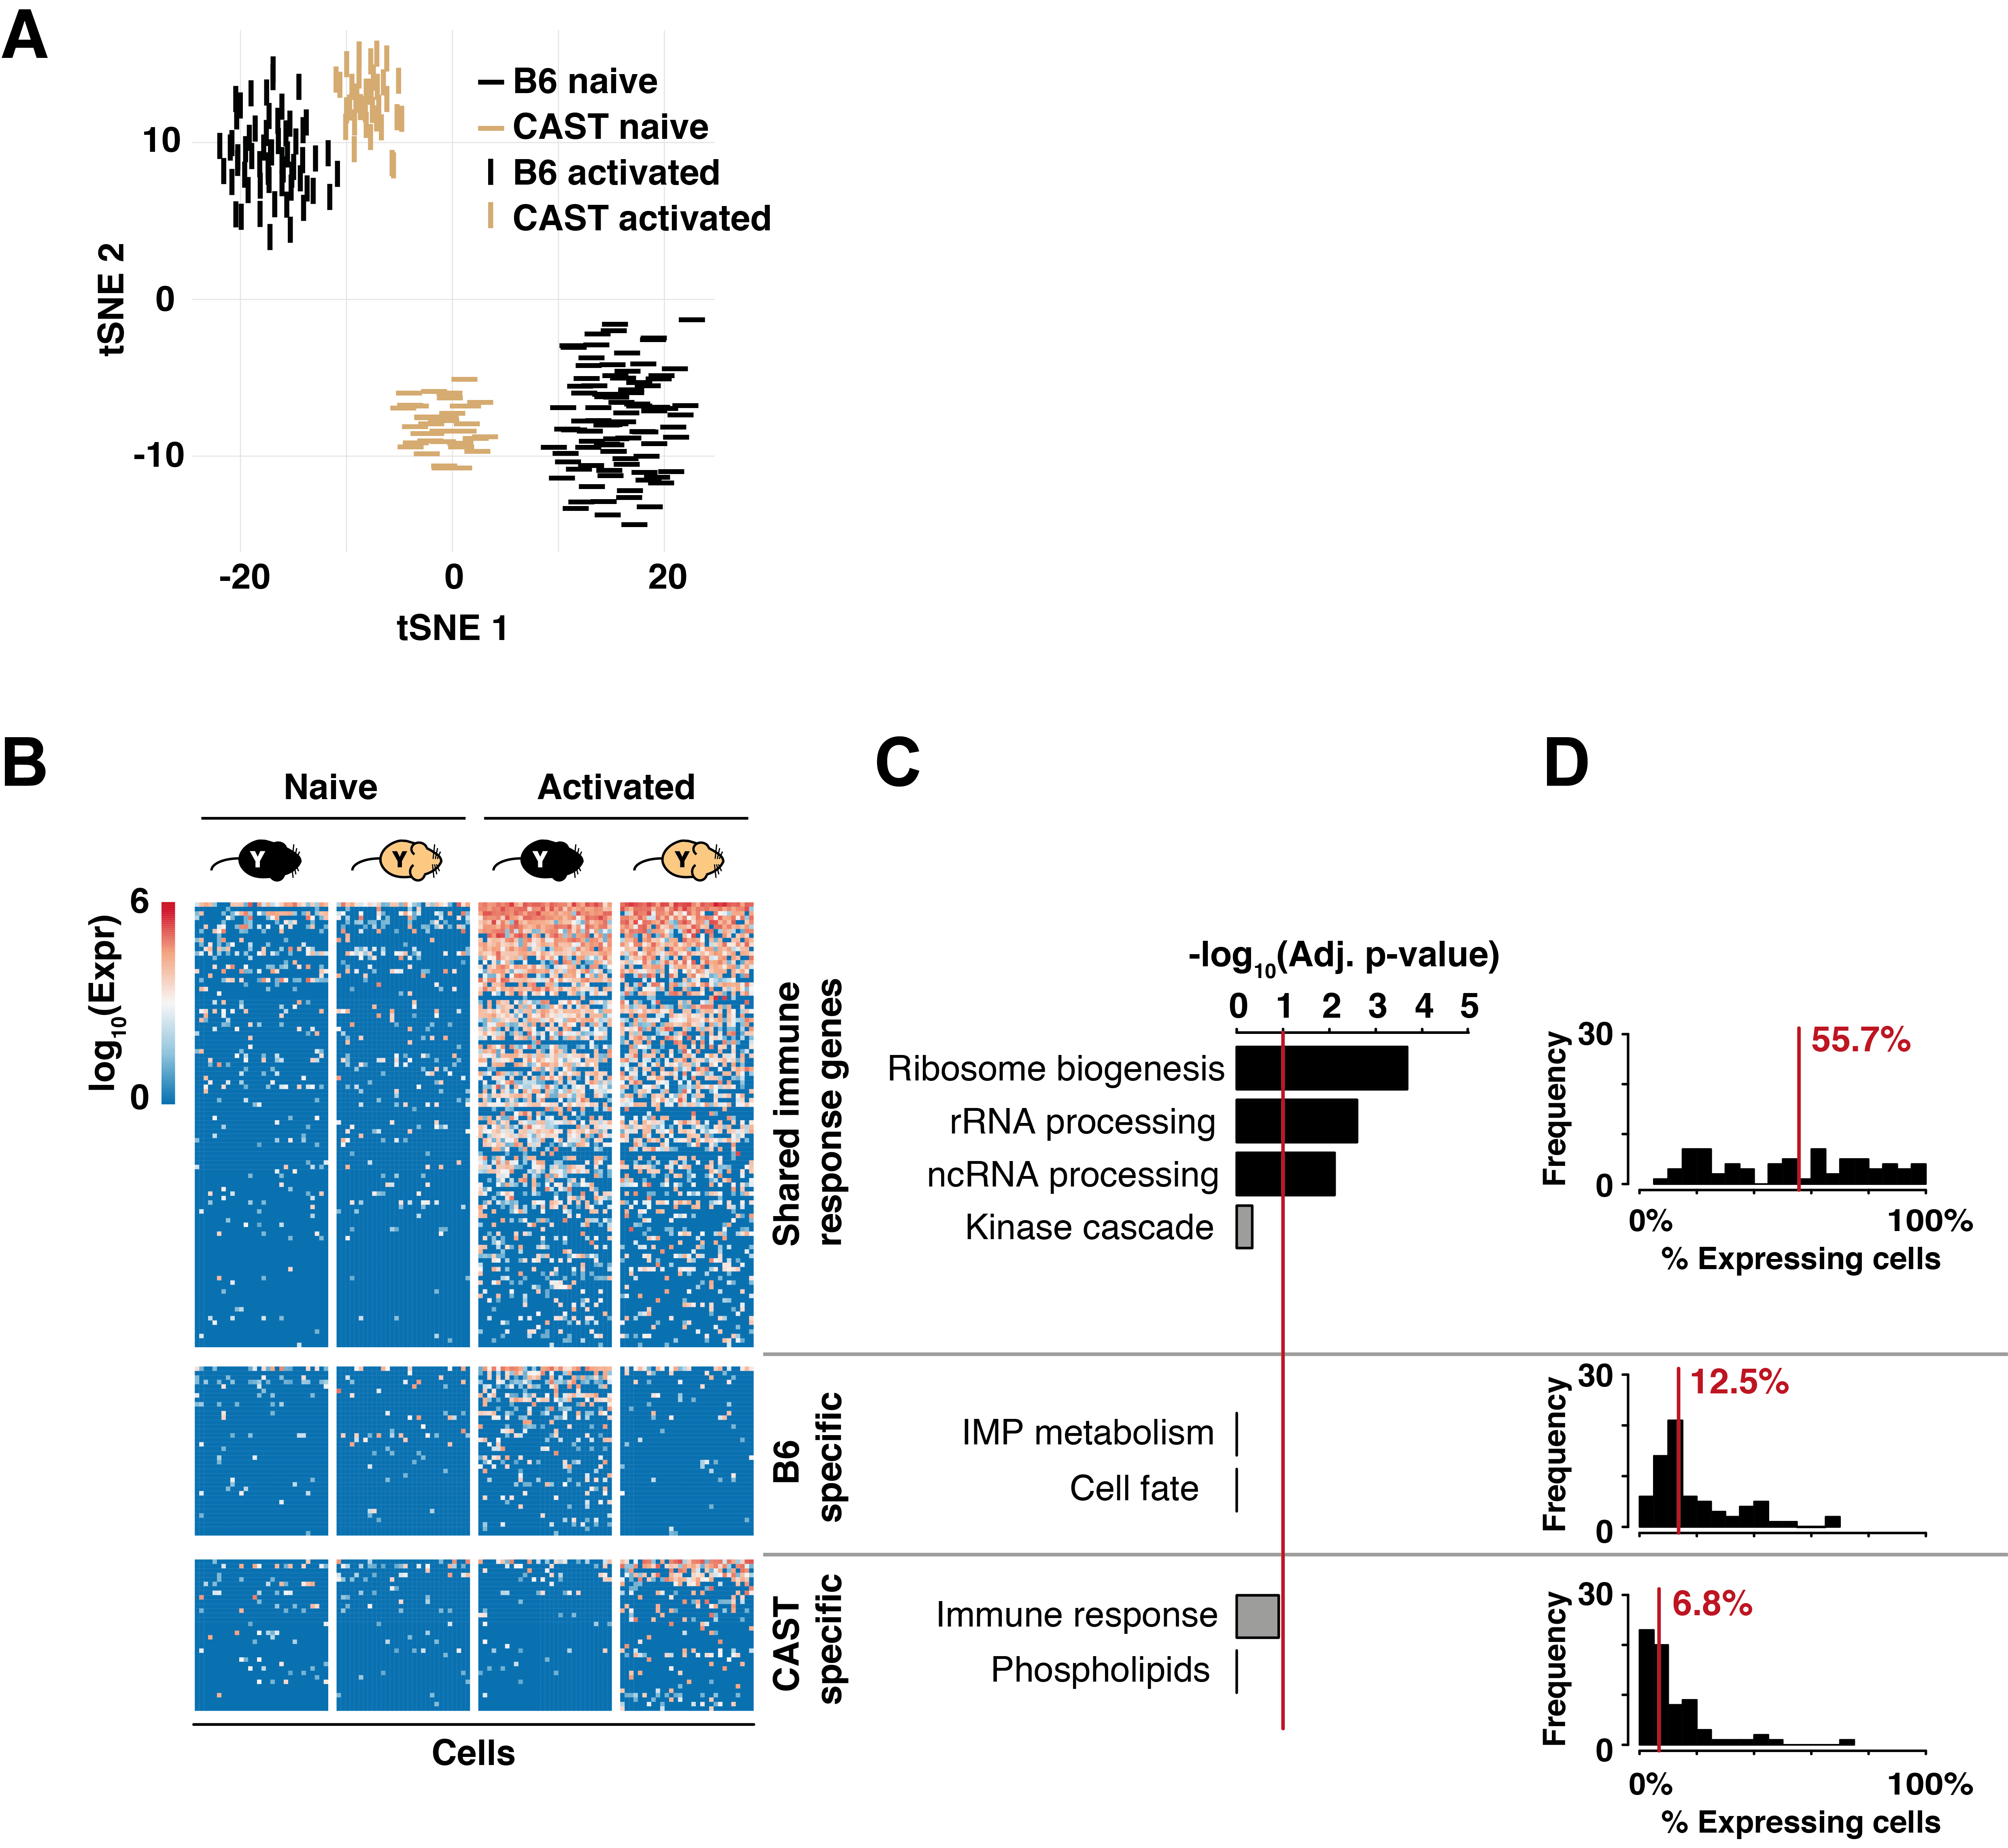
\includegraphics[width=\textwidth]{Fig_11.png}
\caption[Dissecting changes in variability driven by expression outliers]{\textbf{Dissecting changes in variability driven by expression outliers.}\\
5 activated CD4\plus{} T cells were combined with a population of 93 naive CD4\plus{} T cells. \textbf{(A)} Distribution of denoised expression counts for \textit{Il2} in a population of naive CD4\plus{} T cells (red) and the mixture population representing a mix of 93 naive and 5 activated CD4\plus{} T cells (blue). Each dot represents a single cell,\textbf{(B)} For the mixed population (93 naive and 5 activated CD4\plus{} T cells), heatmap of denoised expression counts for all genes highlighted to have increased mean expression and increased variability in the mixed population.}
\label{fig2:mixture_population}
\end{figure}

In summary, our approach allows us to extend the findings from the previous chapter, dissecting immune-response genes into two functional sets: (i) homogeneous up-regulation of biosynthetic machinery components and (ii) heterogeneous up-regulation of several immunoregulatory genes.

\newpage

\subsection{Expression dynamics during \textit{in vivo} CD4\plus{} T cell differentiation}

In contrast to the quick transcriptional switch that occurs within hours of naive T cell activation, transcriptional changes during cellular differentiation processes are more subtle and were found to be coupled with changes in variability prior to cell fate decisions \citep{Richard2016, Mojtahedi2016}. Here, we apply our method to study changes in expression variability during CD4\plus{} T cell differentiation after malaria infection using the dataset introduced by L\"onnberg \emph{et al.} \cite{Lonnberg2017}. In particular, we focus on samples collected 2, 4 and 7 days post-malaria infection, for which more than 50 cells are available. For each condition independently, the BASiCS model was run for 40,000 iterations.\\

\subsubsection{Changes in variability over the differentiation time-course}

First, we studied global changes in over-dispersion along the differentiation time course by comparing posterior estimates for the gene-specific over-dispersion parameter $\delta_i$, focusing on 126 genes for which mean expression does not change \textbf{(Fig.~\ref{fig2:immune_differentiation}A)}. These genes were detected by testing changes in mean expression using a stringent threshold ($\tau_0=0$) between day 2 and day 4 as well as between day 4 and day 7. Genes that are not detected as differentially expressed in both tests were considered for variability analysis. We detect that the expression of these genes is most tightly regulated at day 4, when cells are in a highly proliferative state. Moreover, between day 4 and day 7, the cell population becomes more heterogeneous. This is in line with the emergence of differentiated Th1 and Tfh cells that was observed by \cite{Lonnberg2017}. \\

Next, we exploited the residual over-dispersion parameters to identify changes in variability (irrespective of changes in mean expression) between consecutive time points. For this, we performed differential variability testing using the default threshold on changes in the residual over-dispersion parameter ($\psi_0 = 0.41$) between day 2 and day 4 as well as between day 4 and day 7. After testing, we excluded all genes that are expressed in fewer than 2 cells in at least one time point form down-stream analysis. Separating the remaining genes by whether their variability increases or decreases ($\psi_0 = 0.41$) between time points revealed four different patterns \textbf{(Fig.~\ref{fig2:immune_differentiation}B)}. These include genes whose variability systematically increases (or decreases) as well as patterns where variability is highest (or lowest) at day 4. 

\newpage

\begin{figure}[!h]
\centering
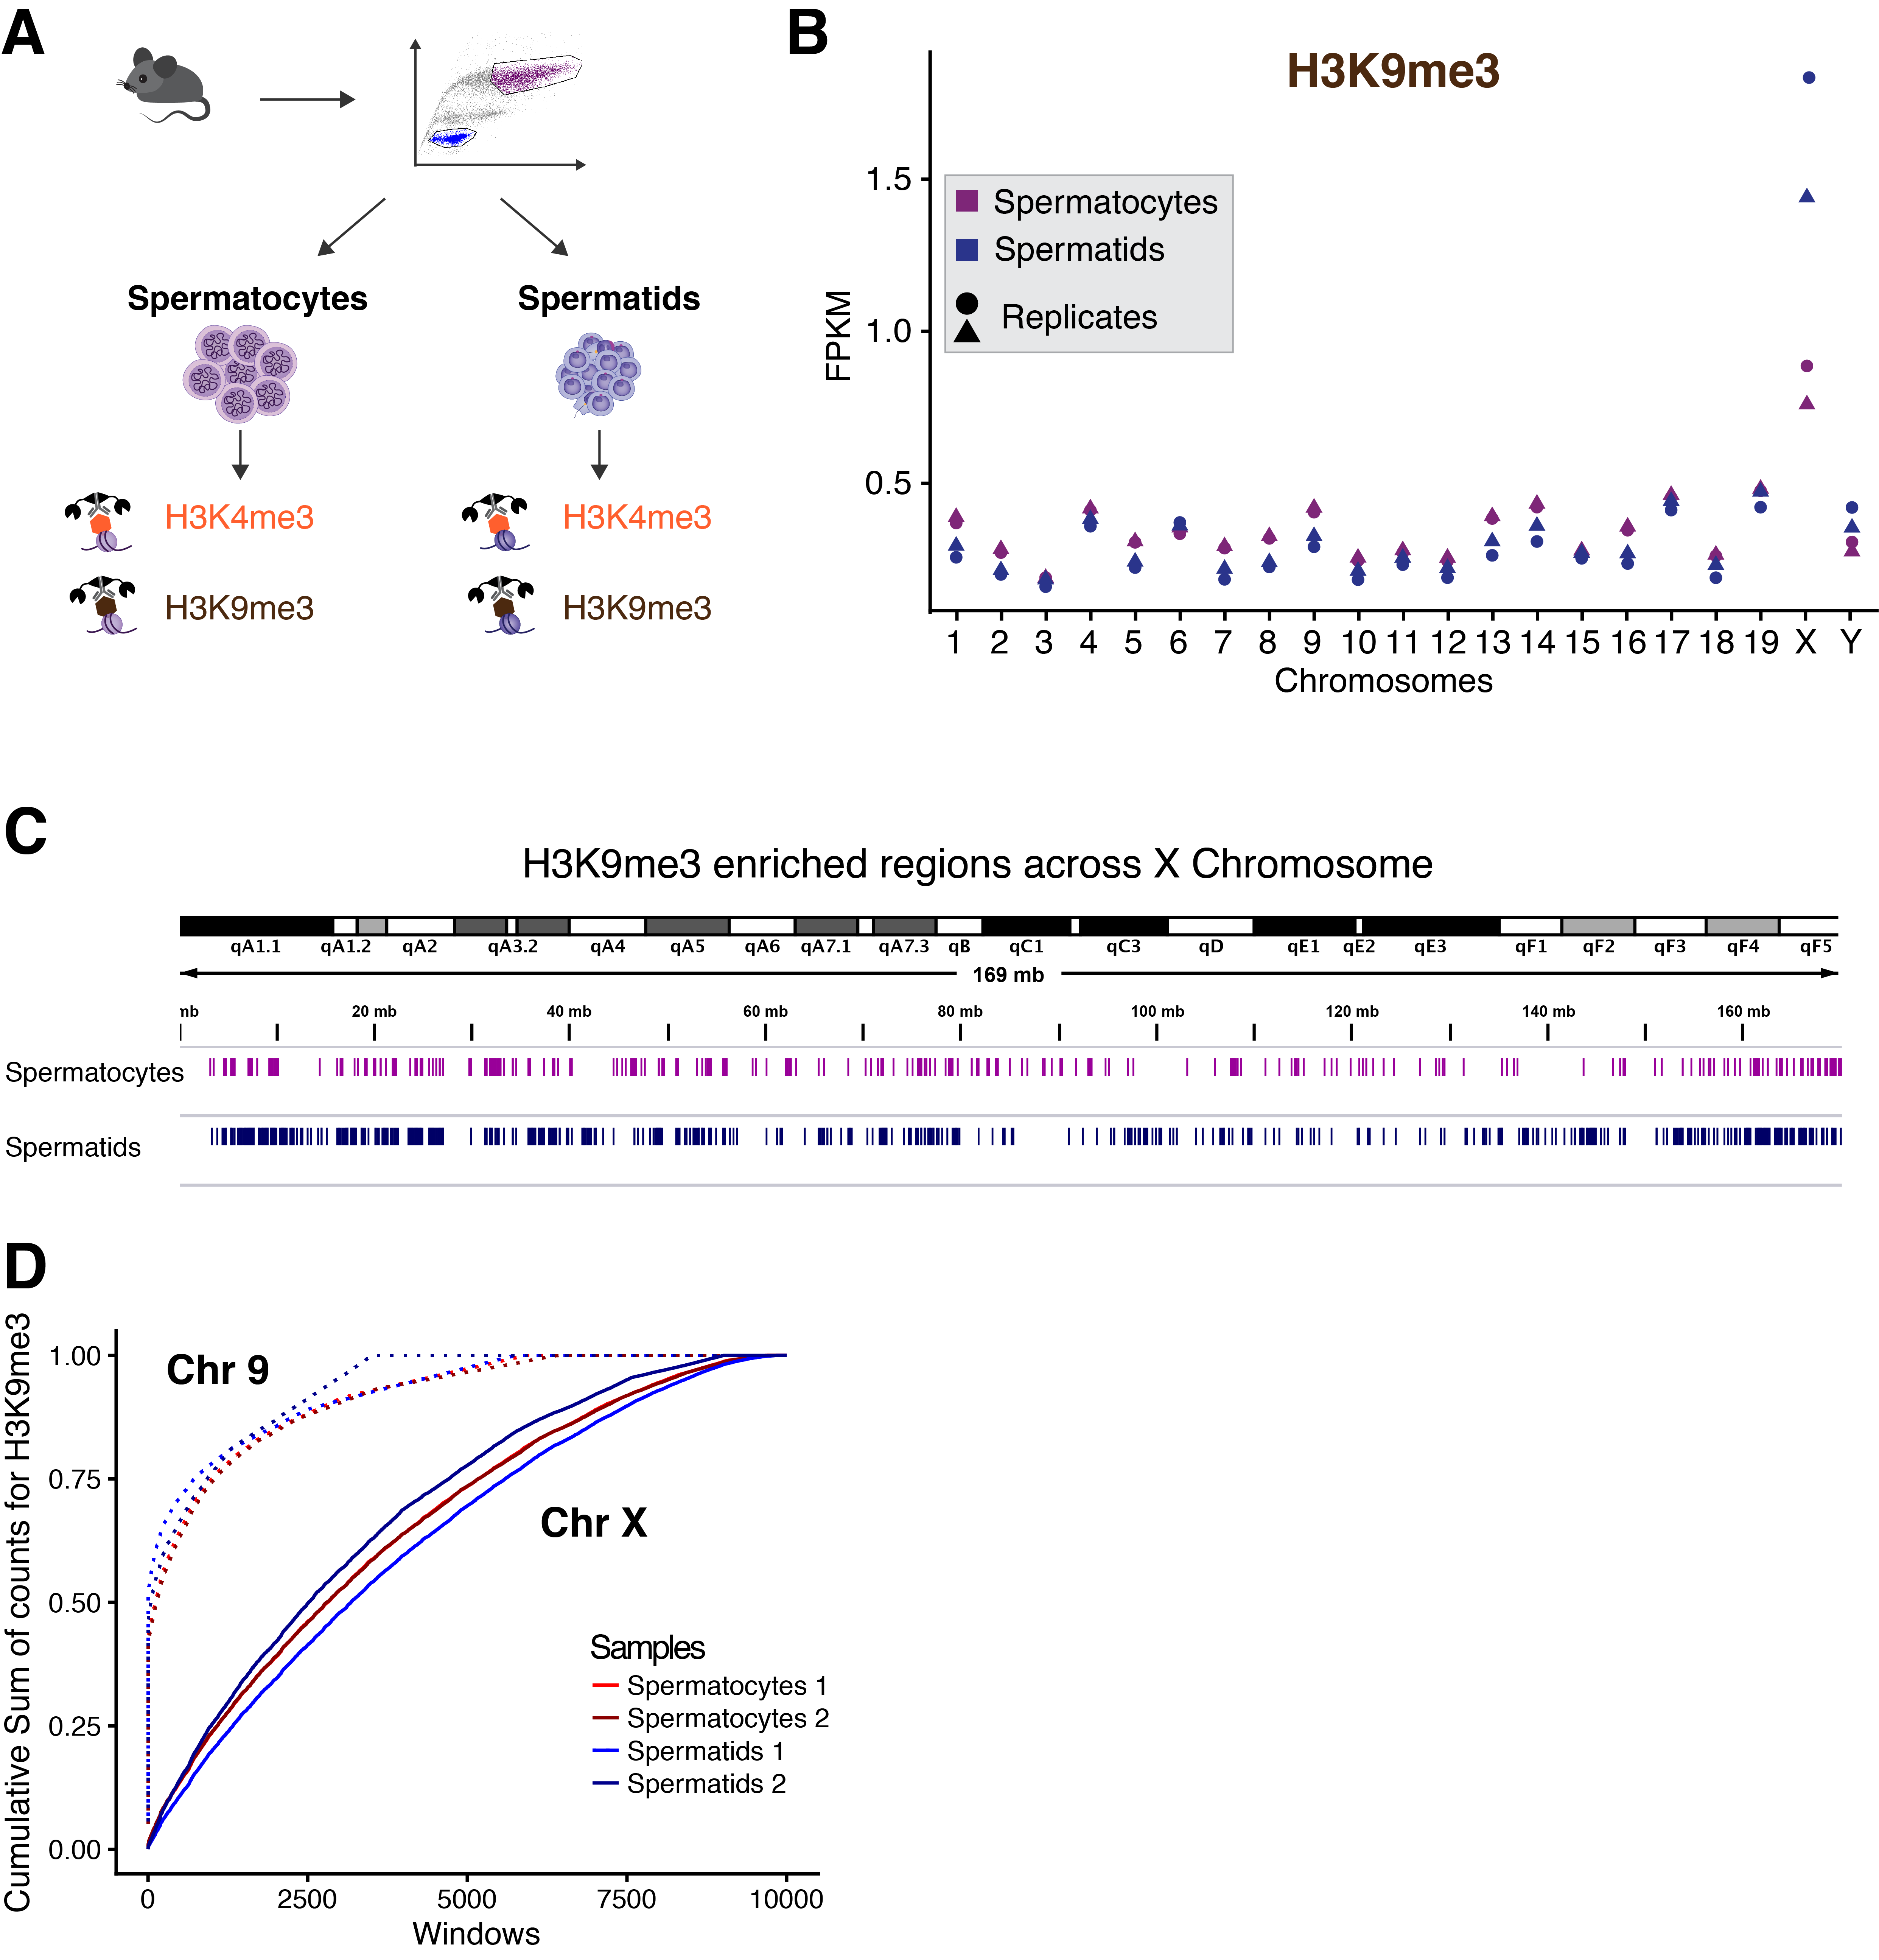
\includegraphics[width=\textwidth]{Fig_12.png}
\caption[Dynamics of expression variability throughout CD4\plus{} T cell differentiation]{\textbf{Dynamics of expression variability throughout CD4\plus{} T cell differentiation.}\\
Analysis was performed on CD4\plus{} T cells assayed 2 days, 4 days and 7 days after \textit{Plasmodium} infection. Changes in residual over-dispersion were tested using a minimum tolerance threshold of $\psi_0=0.41$ (expected false discovery rate is fixed at 10\%). \textbf{(A)} Distribution of posterior estimates of over-dispersion parameters $\delta_i$ for genes that exhibit no changes in mean expression across the differentiation time course. Changes in mean expression were tested using a minimum tolerance threshold of $\tau_0=0$ (expected false discovery rate is fixed at 10\%). \textbf{(B)} Posterior estimates for residual over-dispersion parameters  $\epsilon_i$, focusing on genes with statistically significant changes in expression variability between time points. Gene set size is indicated for each plot.\textbf{(C-D)} Denoised expression counts across cell populations at day 2 (yellow) and day 4 (red) post infection is visualized for representative genes that (C) increase or (D) decrease in variability during differentiation. Each dot represents a single cell.\\}
\label{fig2:immune_differentiation}
\end{figure}

\newpage

\subsubsection{Opposing expression dynamics of lineage-defining marker genes}

The differential variability analysis between day 2 and day 4, revealed  changes in expression variability for a set of immune-related genes \textbf{(Fig.~\ref{fig2:immune_differentiation}C-D)}. For example, expression of \textit{Cxcr5} which encodes the chemokine receptor that directs Tfh cells to the B cell follicles \citep{Crotty2014}, strongly increases in variability on day 4. This finding agrees with results from \cite{Lonnberg2017}, where Tfh and Th1 differentiation was observed to be transcriptionally detectable at day 4 within a subset of activated cells. A similar behaviour was observed for \textit{Tyk2} and \textit{Tigit}. The latter encodes a receptor that is expressed by a subset of Tfh cells and that was found to promote Tfh function \citep{Godefroy2015}. In contrast, we observe a decrease in variability between day 2 and day 4 for \textit{Ikzf4} (Treg-associated gene), \textit{Ly6c1} (expressed by effector T cells) and \textit{Tbx21} (encoding the Th1 lineage-defining transcription factor Tbet). \\

We next selected gene sets listed in \cite{Lonnberg2017} to visualize their changes in mean expression and residual over-dispersion. The first set of genes is taken from Figure 3E of the original publication, which filtered genes based on their association with the bifurcation of Th1 and Tfh differentiation. The second set of genes with sequential peak expression over pseudotime is taken from Figure 5A of the original publication, which were selected based on immunological relevance from a list of dynamic genes during \textit{in vivo} differentiation. For the genes that were detected to be lineage-associated, we detected a continuous increase in expression of Th1-associated genes but not Tfh-associated genes \textbf{(Fig.~\ref{fig2:immune_differentiation2}A)} with the majority of changes in variability for these genes occurring between day 2 and day 4. \\

Finally, we examined immune-related genes (\textit{Il2ra, Tbx21, Il2rb, Cxcr5, Selplg, Id2, Ifng, Icos, Ifngr1}) that were previously described as showing differences in their peak expression over the pseudo time-course of differentiation \citep{Lonnberg2017} \textbf{(Fig.~\ref{fig2:immune_differentiation2}B)}. From this list, the lineage-associated genes \textit{Tbx21} and \textit{Cxcr5} are up-regulated between days 2 and 4. However, these genes  exhibit opposite behaviours in terms of variability: \textit{Cxcr5} increases and \textit{Tbx21} decreases in variability between day 2 and day 4 \textbf{(Fig.~\ref{fig2:immune_differentiation2}C)}. The fact that variability of \textit{Tbx21} (Tbet) expression was highest on day 2 suggests that Tbet is up-regulated very early in differentiation, as seen in \cite{Lonnberg2017} and similar to \textit{in vitro} Th1 induction \citep{Szabo2000}. Moreover, this suggests that Th1 fate decisions (for at least a subset of cells) may be made even earlier than the differentiation bifurcation point identified on day 4 by the original study \citep{Lonnberg2017}. 

\newpage

\begin{figure}[!h]
  \begin{minipage}[c]{0.57\textwidth}
    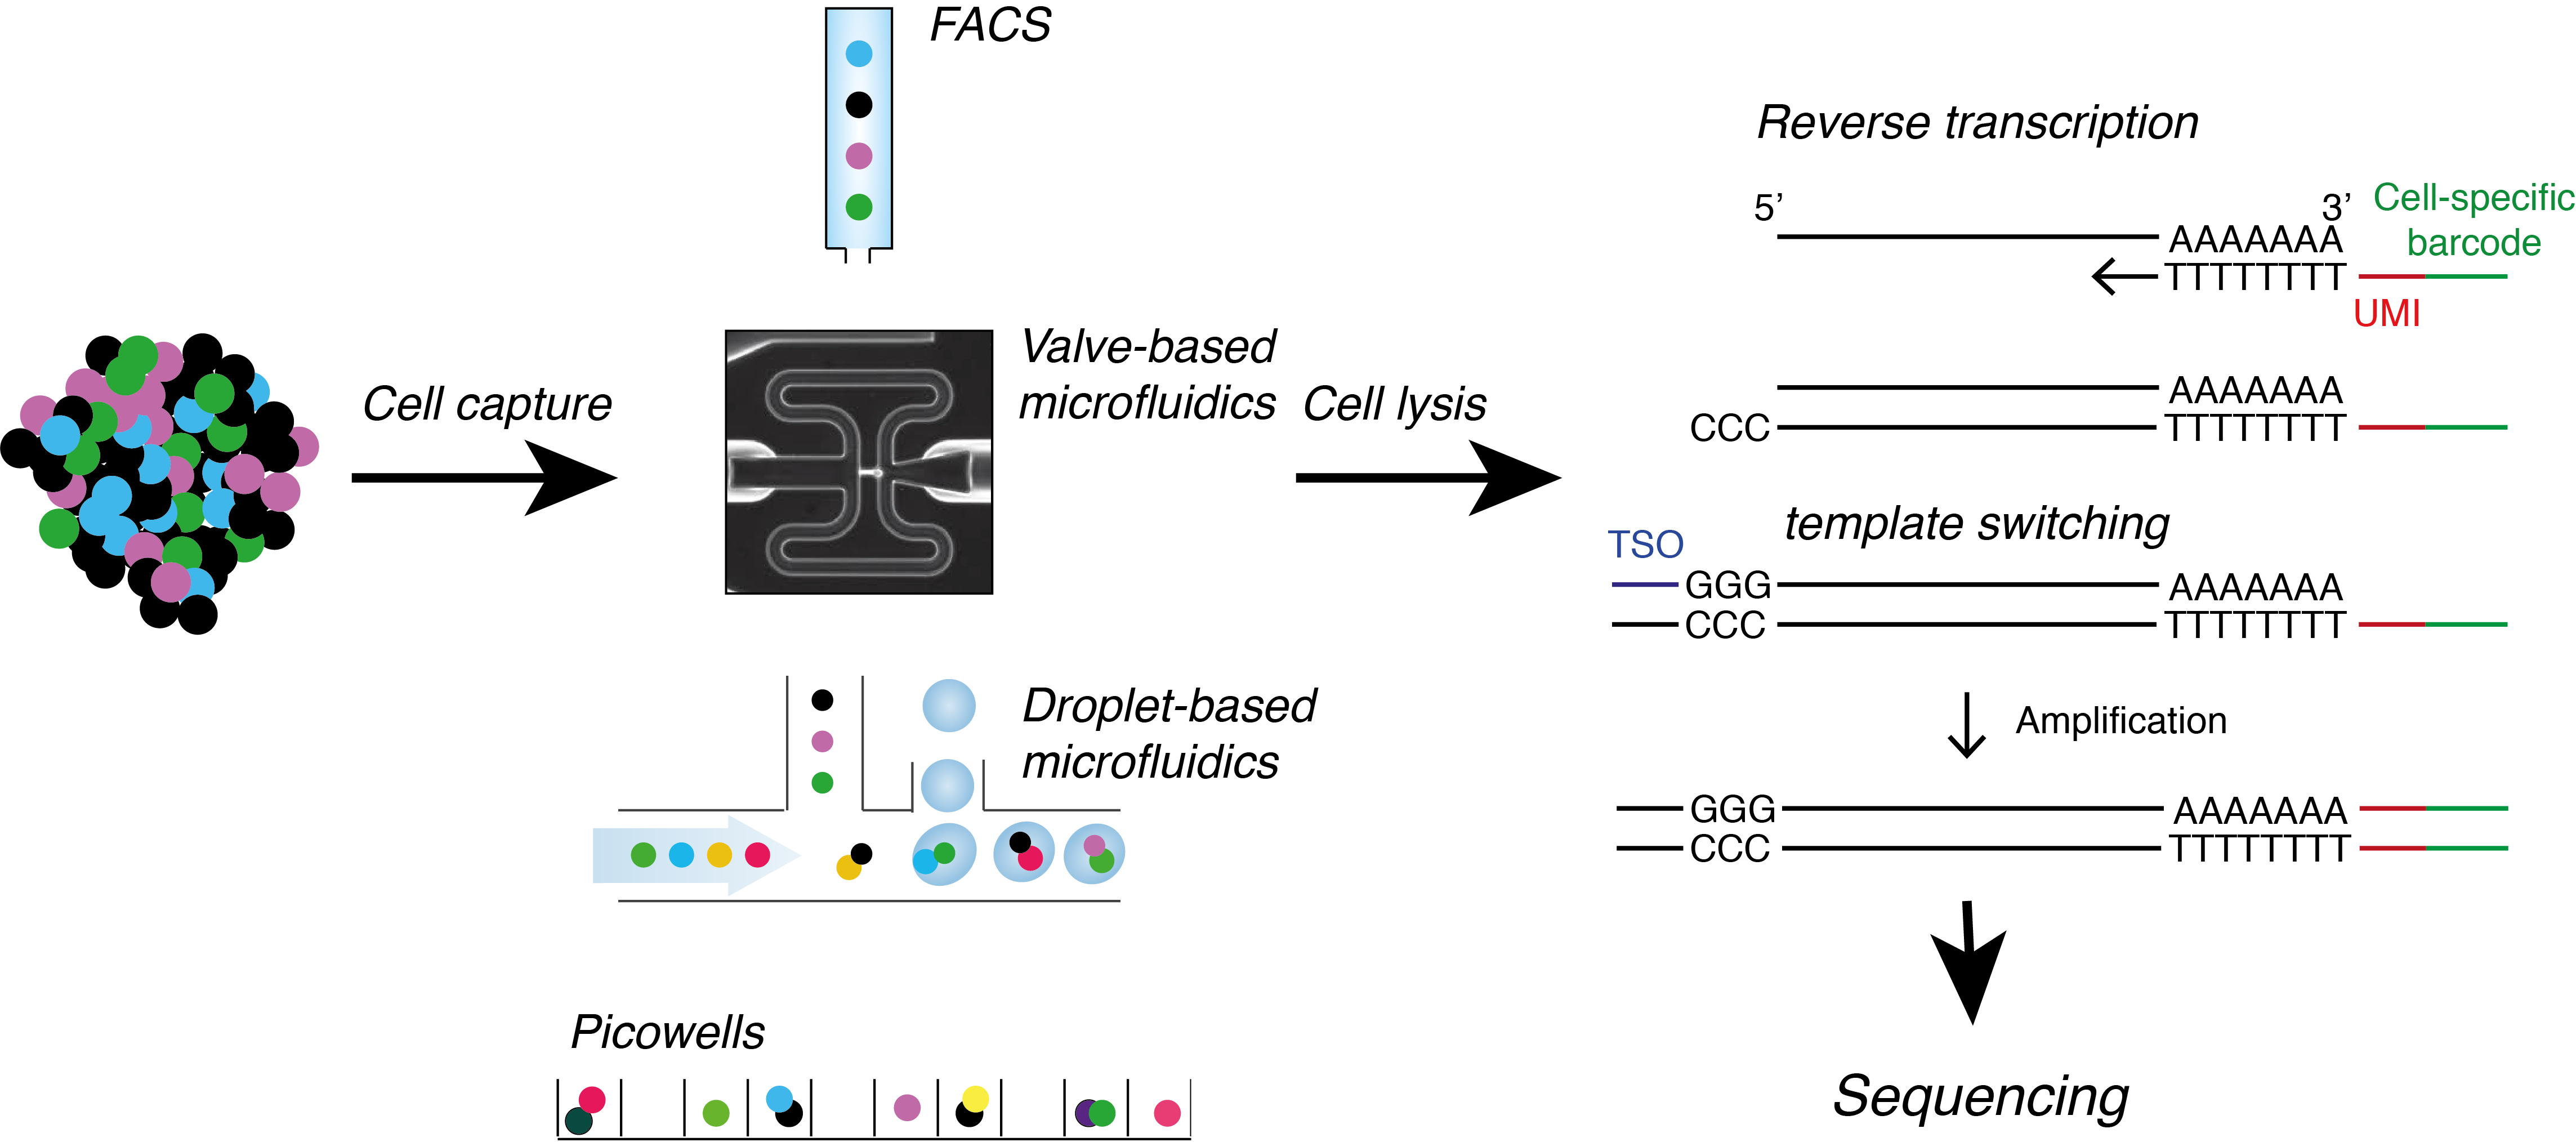
\includegraphics[width=\textwidth]{Fig_13.png}
  \end{minipage}\hfill
  \begin{minipage}[c]{0.4\textwidth}
\caption[Differential regulation of lineage-associated genes across differentiation]{\textbf{Differential regulation of Th1- and Tfh-associated genes across the differentiation process.}\\
Differential mean expression testing (minimum tolerance threshold $\tau_0=1$) and differential residual over-dispersion testing (minimum tolerance threshold $\psi_0=0.41$) was performed on cell populations between day 2 and day 4 as well as day 4 and day 7 controlling the EFDR to 10\%. Genes that increase in expression over time are marked with a red dot while genes that decrease in expression over time are marked with a blue dot. Similarly, genes that increase in variability over time are marked in purple while genes that decrease in variability over time are marked in green. Only genes that pass filtering are visualized. \textbf{(A)} Differential testing results are visualized for Th1- and Tfh-associated genes taken from Figure 3E in \cite{Lonnberg2017}. Genes are ordered based on their correlation with the Th1 trend assignment (top to bottom) or their correlation to Tfh trend assignment (bottom to top).\textbf{(B)} Differential testing results are visualized for important genes during CD4\plus{} T cell differentiation \citep[taken from Figure 5A in][]{Lonnberg2017}. Genes were ordered based on their peak expression point in pseudotime as defined by \cite{Lonnberg2017}. \textbf{(C)}\textit{Tbx21} (blue) and \textit{Cxcr5} (red) measured at day 2, day 4 and day 7 post-infection. Posterior estimates for residual over-dispersion parameters $\epsilon_i$ are plotted against posterior estimates for mean expression parameters $\mu_i$. Statistically significant changes in mean expression (DE, minimum tolerance threshold of $\tau_0=1$) and variability (DV, minimum tolerance threshold of $\psi_0=0.41$) are indicated for each comparison} \label{fig2:immune_differentiation2}
  \end{minipage}
\end{figure}

\newpage

\section{Application to droplet-based scRNA-Seq data}

\begin{Comment}
\textbf{Declaration} In the context of expanding the BASiCS framework to test changes in variability in parallel to changes in mean expression, Catalina A. Vallejos (The Alan Turing Institute/MRC Institute of Human Genetics/University of Edinburgh) developed an approach where technical variation was quantified by borrowing information across multiple replicates. This avoids the use of technical spike-in genes when droplet-based scRNA-Seq data is analysed. This approach is part of the publication:\\

Nils Eling, Arianne C. Richard, Sylvia Richardson, John C. Marioni, Catalina A. Vallejos. Robust expression variability testing reveals heterogeneous T cell responses. \emph{Cell Systems}, In press, 2018 \\

Here, I will not describe this approach in detail as this has not been my own work but it integrates with my contribution to assess mean-independent changes in variability for droplet-based scRNA-Seq data.
\end{Comment}

With the development of droplet-based scRNA-Seq technologies the number of cells that can be profiled per experiment strongly increased with the cost of lower sequencing depth per cell \citep{Macosko2015, Klein2015, Zheng2017}. Furthermore, these technologies don't allow the use of technical spike-in RNA to measure technical variation \citep{Brennecke2013}. The initial BASiCS model \citep{Vallejos2015BASiCS, Vallejos2016} quantifies technical variation through a vertical data integration approach, exploiting a set of synthetic RNA spike-in molecules (e.g.~\citep{Jiang2011}). To ensure the broad applicability of the BASiCS model, both the regression and non-regression models have been expanded to 
handle datasets without spike-in genes. For this purpose, principles of measurement error models were exploited, where --- in the absence of gold standard features --- technical variation is quantified through {\it replication} \citep{Carroll1998}. This horizontal data integration approach is based on experimental designs where cells from a population are randomly allocated to multiple independent experimental replicates (batches). In such an experimental design, the no-spikes implementation of BASiCS assumes that biological effects are shared across batches and that technical variation will be reflected by spurious differences.  As shown in the original publication, posterior inference under the no-spikes BASiCS model closely matches the original implementation for datasets where spike-ins and batches are available. Technical details about the no-spikes implementation of BASiCS are discussed in the original publication (see \textbf{Declaration}).

\newpage

\subsection{Differential testing using somitic and pre-somitic mesoderm cells}

To test the applicability of the regression BASiCS model to droplet-based scRNA-Seq data, I analysed cells isolated from mouse embryos at post-natal day (E)4.28 \citep{Ibarra-Soria2018}. Ibarra-Soria \emph{et al.} analysed more than 20,000 cells to identify the major cell types following gastrulation. Key findings included a spatial sub-structure within the foregut, detection of oscillating gene expression patterns during somitogenesis and the contribution of the leukotriene pathway to blood formation.  We selected the cells identified as presomotic mesoderm and somitic mesoderm as test populations which reside in contrasting differentiation stages. Somitogenesis is a rhythmic and sequential differentiation process from pre-somitic mesoderm (PSM) cells to mature somites which later on give rise to bone, muscle and skin of the adult body. throughout this process, oscillating gene expression patterns control the differentiation of PSM into somitic mesoderm (SM). Driving factors for this are Wnt and fibroblast growth factor (FGF) signalling on the side of the PSM and retinoic acid signalling in somites \cite{Oates2012}. The regression BASiCS model can now further dissect transcriptional regulation between these groups of cells.

\subsubsection{Data processing}

The raw counts data and assigned cluster labels can be obtained from ArrayExpress [E-MTAB-6153]. I selected cells labelled as pre-somitic mesoderm and somitic mesoderm for further down-stream analysis. PCA shows a clear separation between these two cells types with an additional intermediate cell type labelled as 'presomiticmesoderm.b'. I excluded this small of cells as well as outlying cells for which $\text{PC2}{}<{}-5$ \textbf{(Fig.~\ref{fig2:droplet}A)}. After filtering, I obtained \todo{XXX} pre-somitic mesoderm cells and \todo{YYY} somitic mesoderm cells for further analysis. For each of the two populations, the MCMC was run for 20,000 iterations separately. After posterior inference was completed, I first confirmed that the model estimated the regression trend between the over-dispersion parameters $\delta_i$ and mean expression parameters $\mu_i$ correctly. For both conditions, the regression trend captures the full range of data point and differential testing can be performed. For differential testing, I used a threshold of $\tau_0=1$ to assess changes in mean expression and the default threshold $\psi_0\approx{}0.41$ to test changes in residual over-dispersion.  

\subsubsection{Changes in mean expression during somitogenesis}

\subsubsection{Changes in variability during somitogenesis}


With this analysis, I confirmed that the regression BASiCS model can be applied to droplet-based scRNA-Seq data to assess changes transcriptional variability between conditions. This is an important validation for the next chapter, where I applied the regression BASiCS model to continuous droplet-based scRNA-Seq data to study changes in variability during spermatogenesis. 

\newpage
%!TEX root = ../chapter2.tex
%******************************
%	 Discussion 
%*****************************

\section{Discussion}

In recent years, the importance of modulating cell-to-cell transcriptional variation within cell populations for tissue function maintenance and development has become apparent \citep{BaharHalpern2015, Mojtahedi2016, Goolam2016}. Here, we present a statistical approach to robustly test changes in expression variability between cell populations using scRNA-Seq data. Our method uses a hierarchical Bayes formulation to extend the BASiCS framework by addressing (increasingly popular) experimental protocols where spike-in sequences are not available and by incorporating an additional set of residual over-dispersion parameters $\epsilon_i$ that are not confounded by changes in mean expression. Together, these extensions ensure a broader applicability of the BASiCS software and allow statistical testing of changes in variability that are not confounded by technical noise or mean expression.  \\ 

In general, stable gene-specific variability estimates ideally require a large and deeply sequenced dataset containing a homogeneous cell population \citep[the use of unique molecular identifiers for quantifying transcript counts can also improve variability estimation, see][]{Grun2014}. However, we observe that the regression BASiCS model leads to more stable inference that requires fewer cells to accurately estimate gene-specific summaries, particularly for lowly expressed genes. Despite this, careful considerations should be taken in extreme scenarios where the number of cells is small and/or the data is highly sparse (e.g.~droplet based approaches). These features of the data not only affect parameter estimation but also downstream differential testing. For sparse datasets with low numbers of cells, we recommend the use of a stringent minimum tolerance threshold and/or calibrating the test to a low expected false discovery rate (e.g.~1\%) to avoid detecting spurious signals. Moreover, if possible, an internal calibration can be performed to find a reasonable minimum tolerance threshold (e.g.~by randomly permuting cells between two groups to calibrate the null distribution of the differences between populations). \\

Our method allows characterisation of the extent and nature of variable gene expression in CD4\plus{} T cell activation and differentiation. Firstly, we observe that during acute activation of naive T cells, genes of the biosynthetic machinery are homogeneously up-regulated, while specific immune-related genes become more heterogeneously up-regulated. In particular, increased variability in expression of the apoptosis-inducing Fas ligand \citep{Strasser2009} and the inhibitory ligand PD-L1 \citep{Chikuma2016} suggests a mechanism by which newly activated cells might suppress re-activation of effector cells, thereby dynamically modulating the population response to activation. Likewise, more variable expression of Smad3, which translates inhibitory TGF$\beta$ signals into transcriptional changes \citep{Delisle2013}, may indicate increased diversity in cellular responses to this signal. Increased variability in \textit{Pou2f2} (Oct2) expression after activation suggests heterogeneous activities of the NF-$\kappa$B and/or NFAT signalling cascades that control its expression \citep{Mueller2013}.
Moreover, we detect up-regulated and more variable \textit{Il2} expression, suggesting heterogeneous IL-2 protein expression, which is known to enable T cell population responses \citep{Fuhrmann2016}. \\

Finally, we studied changes in gene expression variability during CD4\plus{} T cell differentiation towards a Th1 and Tfh cell state over a 7 day time course after \textit{in vivo} malaria infection \citep{Lonnberg2017}. Our analysis provides several insights into this differentiation system. Firstly, we observe a tighter regulation in gene expression among genes that do not change in mean expression during differentiation at day 4 at which divergence of Th1 and Tfh differentiation was previously identified \citep{Lonnberg2017}. This decrease in variability on day 4 is potentially due to induction of a strong pan-lineage proliferation program. However, we observe that not all genes follow this trend and uncover four different patterns of variability changes. Secondly, we observe that several Tfh and Th1 lineage-associated genes change in expression variability between days 2 and 4. For example, we noted a decrease in variability for one key Th1 regulator, \textit{Tbx21} (encoding Tbet), which suggests that a subset of cells may have already committed to the Th1 lineage at day 2. Three additional Th1 lineage-associated genes also followed this trend (\textit{Ahnak}, \textit{Ctsd}, \textit{Tmem154}). These data suggest that differentiation fate decisions may arise as early as day 2 in subpopulations within this system, resulting in high gene expression variability. Such an effect is in accordance with the early commitment to effector T cell fates that was previously observed during viral infection \citep{Choi2011}. As these results illustrate, diversity in differentiation state within a population of T cells can drive our differential variability results. To further disect these results, subsequent analyses such as the pseudotime inference used in \cite{Lonnberg2017} could be used to characterize a continuous differentiation process.\\

In sum, our model provides a robust tool for understanding the role of heterogeneity in gene expression during cell fate decisions. With the increasing use of scRNA-Seq to study this phenomenon, our and other related tools will become increasingly important.





%!TEX root = ../main.tex
%******************************
%	 Chapter 3
%*****************************

\chapter{Transcriptional dynamics during spermatogenesis at single-cell resolution}  

\graphicspath{{"../../Dropbox (Cambridge  University)/Figures_for_thesis/Chapter3/"}}

\begin{Abstract}
Spermatogenesis is a recurring differentiation process that results in the production of male gametes within the testes. Consequently, its in-depth characterisation is needed to understand male fertility. During spermatogenesis, spermatogonial stem cells undergo a unidirectional differentiation process to form spermatocytes, round spermatids and lastly mature sperm. This process involves a complex sequence of developmental steps and is coupled to large-scale chromatin rearrangements, therefore making it difficult to profile.
To address this, we thoroughly characterised spermatogenesis by   profiling the transcriptomes of over 20,000 cells that were captured using droplet-based scRNA-Seq. To confidently connect transcriptional profiles to distinct developmental stages, we profiled multiple time-points during the first wave of spermatogenesis. As juvenile animals progress through spermatogenesis for the first time, development has only progressed to a certain point, thus allowing the identification of the most mature cell type. With this precise labelling, we can dissect developmental processes such as spermatogonial differentiation, meiosis and spermiogenesis at a molecular level. Furthermore, our data captured the expression dynamics of the X chromosome, which is subject to meiotic silencing in spermatocytes, followed by a partial reactivation in spermatids. ScRNA-Seq reveals the distinct temporal expression dynamics present in the post-meiotic reactivation of the X chromosome. Profiling of the associated chromatin changes identified a set of genes specifically repressed by H3K9me3 in spermatocytes that later-on escape post-meiotic silencing in spermatids, demonstrating extensive chromatin remodelling on the X chromosome. After fully characterising spermatogenesis at a single-cell level, BASiCS was used to detect changes in transcriptional variability by estimating the residual over-dispersion measures for the different germ cell populations. In this analysis, the differentiation trajectory defines a new confounding factor that must be accounted for to accurately quantify variability in gene expression levels.  
\end{Abstract}

\newpage

\vspace*{\fill}

\begin{Comment}
\textbf{Declaration} This project was done in collaboration with members of the Marioni and Odom lab. Christina Ernst performed all wet-lab experiments presented in this chapter. Celia P. Martinez-Jimenez performed preliminary experiments. John Marioni and Duncan Odom supervised the study. Christina Ernst, I, John Marioni and Duncan Odom designed the study and wrote the manuscript. I performed all computational analyses and produced all figures in this chapter (except the histology images and schematics). The last section of this chapter is purely my own contribution. The preprint has been made available online at:\\

Christina Ernst$^\ast$, Nils Eling$^\ast$, Celia P. Martinez-Jimenez, John C. Marioni, Duncan T. Odom. Staged developmental mapping and X chromosome transcriptional dynamics during mouse spermatogenesis. \emph{bioRxiv}, 2018, ($^\ast$ equal contributions)
\end{Comment}

\vspace*{\fill}

\begin{figure}[hb]
\centering    
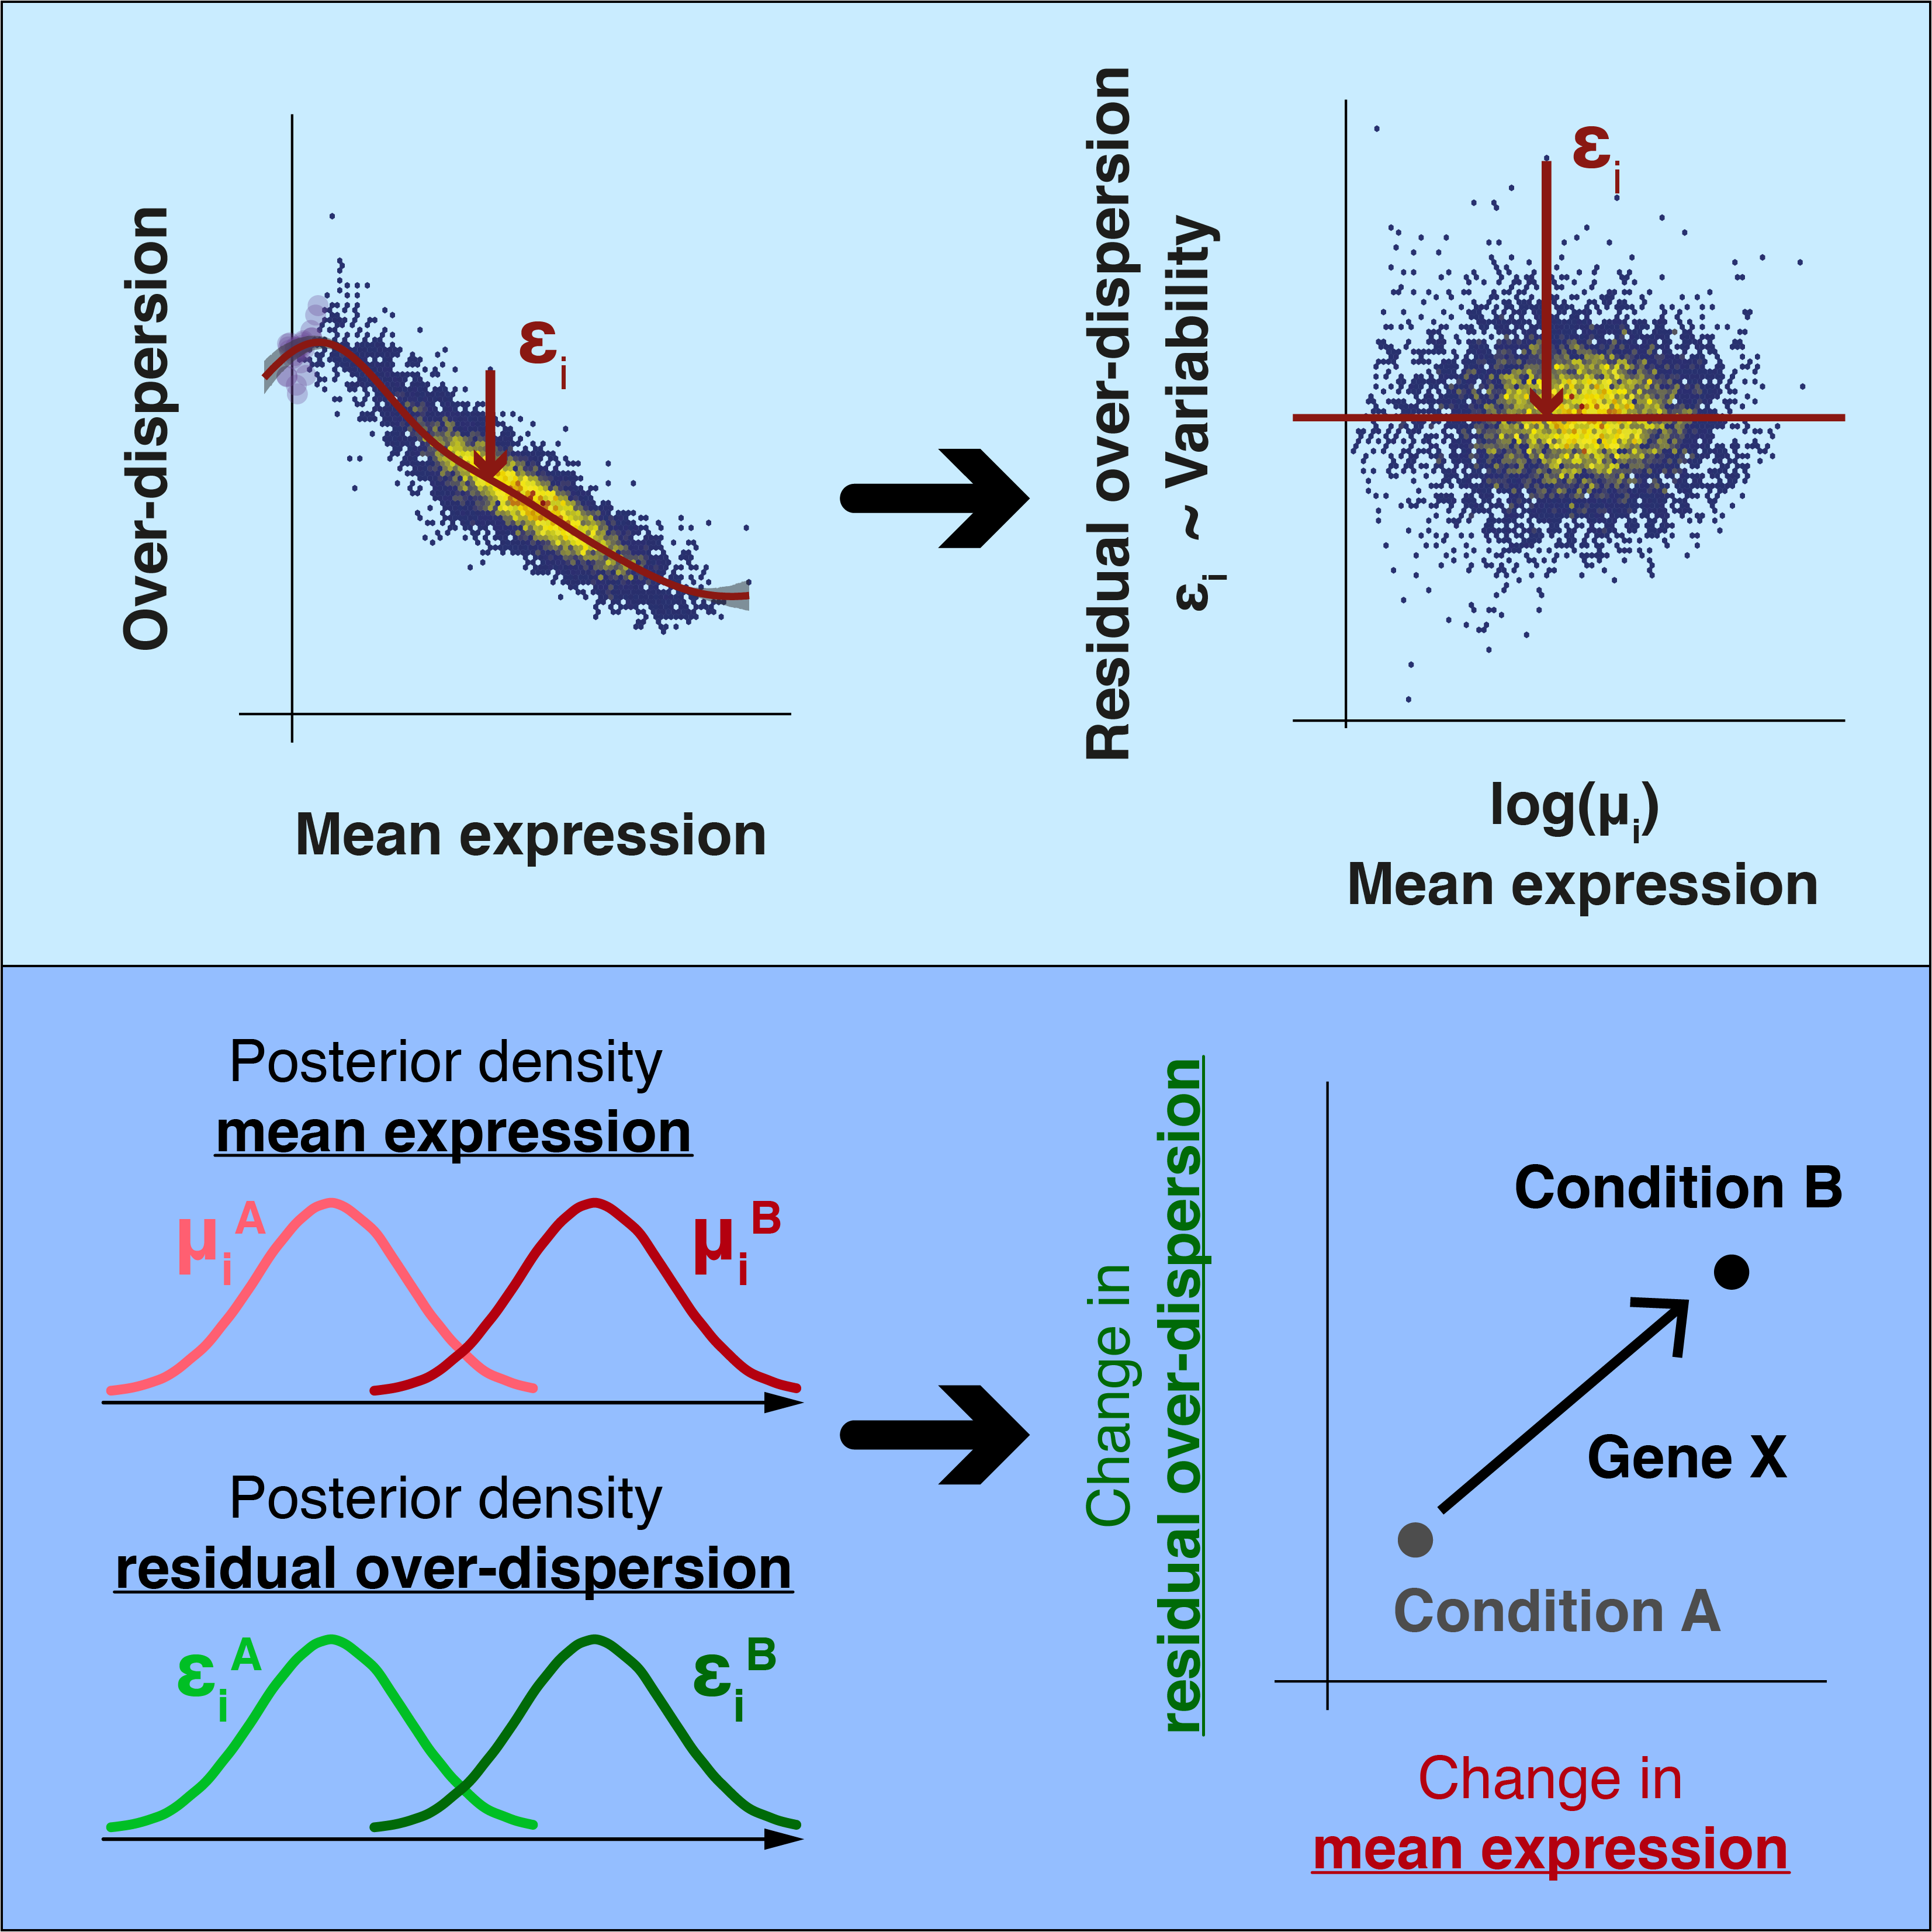
\includegraphics[width=\textwidth]{GraphicalAbstract.png}
\caption*{}
\end{figure}

\vspace*{\fill}


\newpage

% Include different main sections of the third chapter
%!TEX root = ../chapter3.tex
%******************************
%	 Introduction 
%*****************************

\section{Introduction}

Gametogenesis is the process which forms haploid gametes that carry one copy of the individuals DNA. Sexual reproduction requires the fusion of two gametes from the opposite sex to drive evolution and adaptation \citep{McDonald2016}. Spermatogenesis, the male version of gametogenesis, is a tightly regulated developmental process to generate mature sperm. 
During spermatogenesis, spermatogonial stem cells undergo a unidirectional differentiation programme to form mature spermatozoa. This process occurs in the epithelium of seminiferous tubules in the testis \textbf{(Fig.~\ref{fig3:cell_staging}B)} and is tightly coordinated to ensure the continuous production of mature sperm cells. In the mouse, the first step involves spermatogonial differentiation to form pre-leptotene spermatocytes \citep{Oakberg1971, DeRooij1973, DeRooij2000}. Pre-leptotene spermatocytes then commit to meiosis, a cell division programme that consists of two consecutive cell divisions to produce haploid cells. To accommodate homologous recombination between sister chromatids and chromosome synapsis \citep{Marston2004}, prophase of meiosis I is extremely prolonged, lasting several days in males. It can be divided into four substages: leptonema (L), zygonema (Z), pachynema (P) and diplonema (D). Following the two consecutive cell divisions, haploid cells known as round spermatids (RS) undergo a complex differentiation programme called spermiogenesis to form mature spermatozoa \citep{Oakberg1956}. \\

Spermatogenesis takes place in a highly orchestrated fashion, with tubules periodically cycling through twelve epithelial stages defined by the combination of germ cells present (see \textbf{Fig.~\ref{fig3:cell_staging}B} and \citep{Oakberg1956}). The completion of one cycle takes 8.6 days in the mouse, and the overall differentiation process from spermatogonia to mature spermatozoa requires approximately 35 days \citep{Oakberg1956a}. Thus, four to five generations of germ cells are present within a tubule at any given time. In adult animals, each tubule resides in a different cycle stage meaning that at any given time-point, the continuum of germ cell types is present in the testis \textbf{(Fig.~\ref{fig3:cell_staging})}. The continuity of this differentiation process and the gradual transitions between spermatogenic cell types have made the isolation and thus the molecular characterisation of individual sub-stages during spermatogenesis difficult.

\newpage

\begin{figure}[!h]
\centering
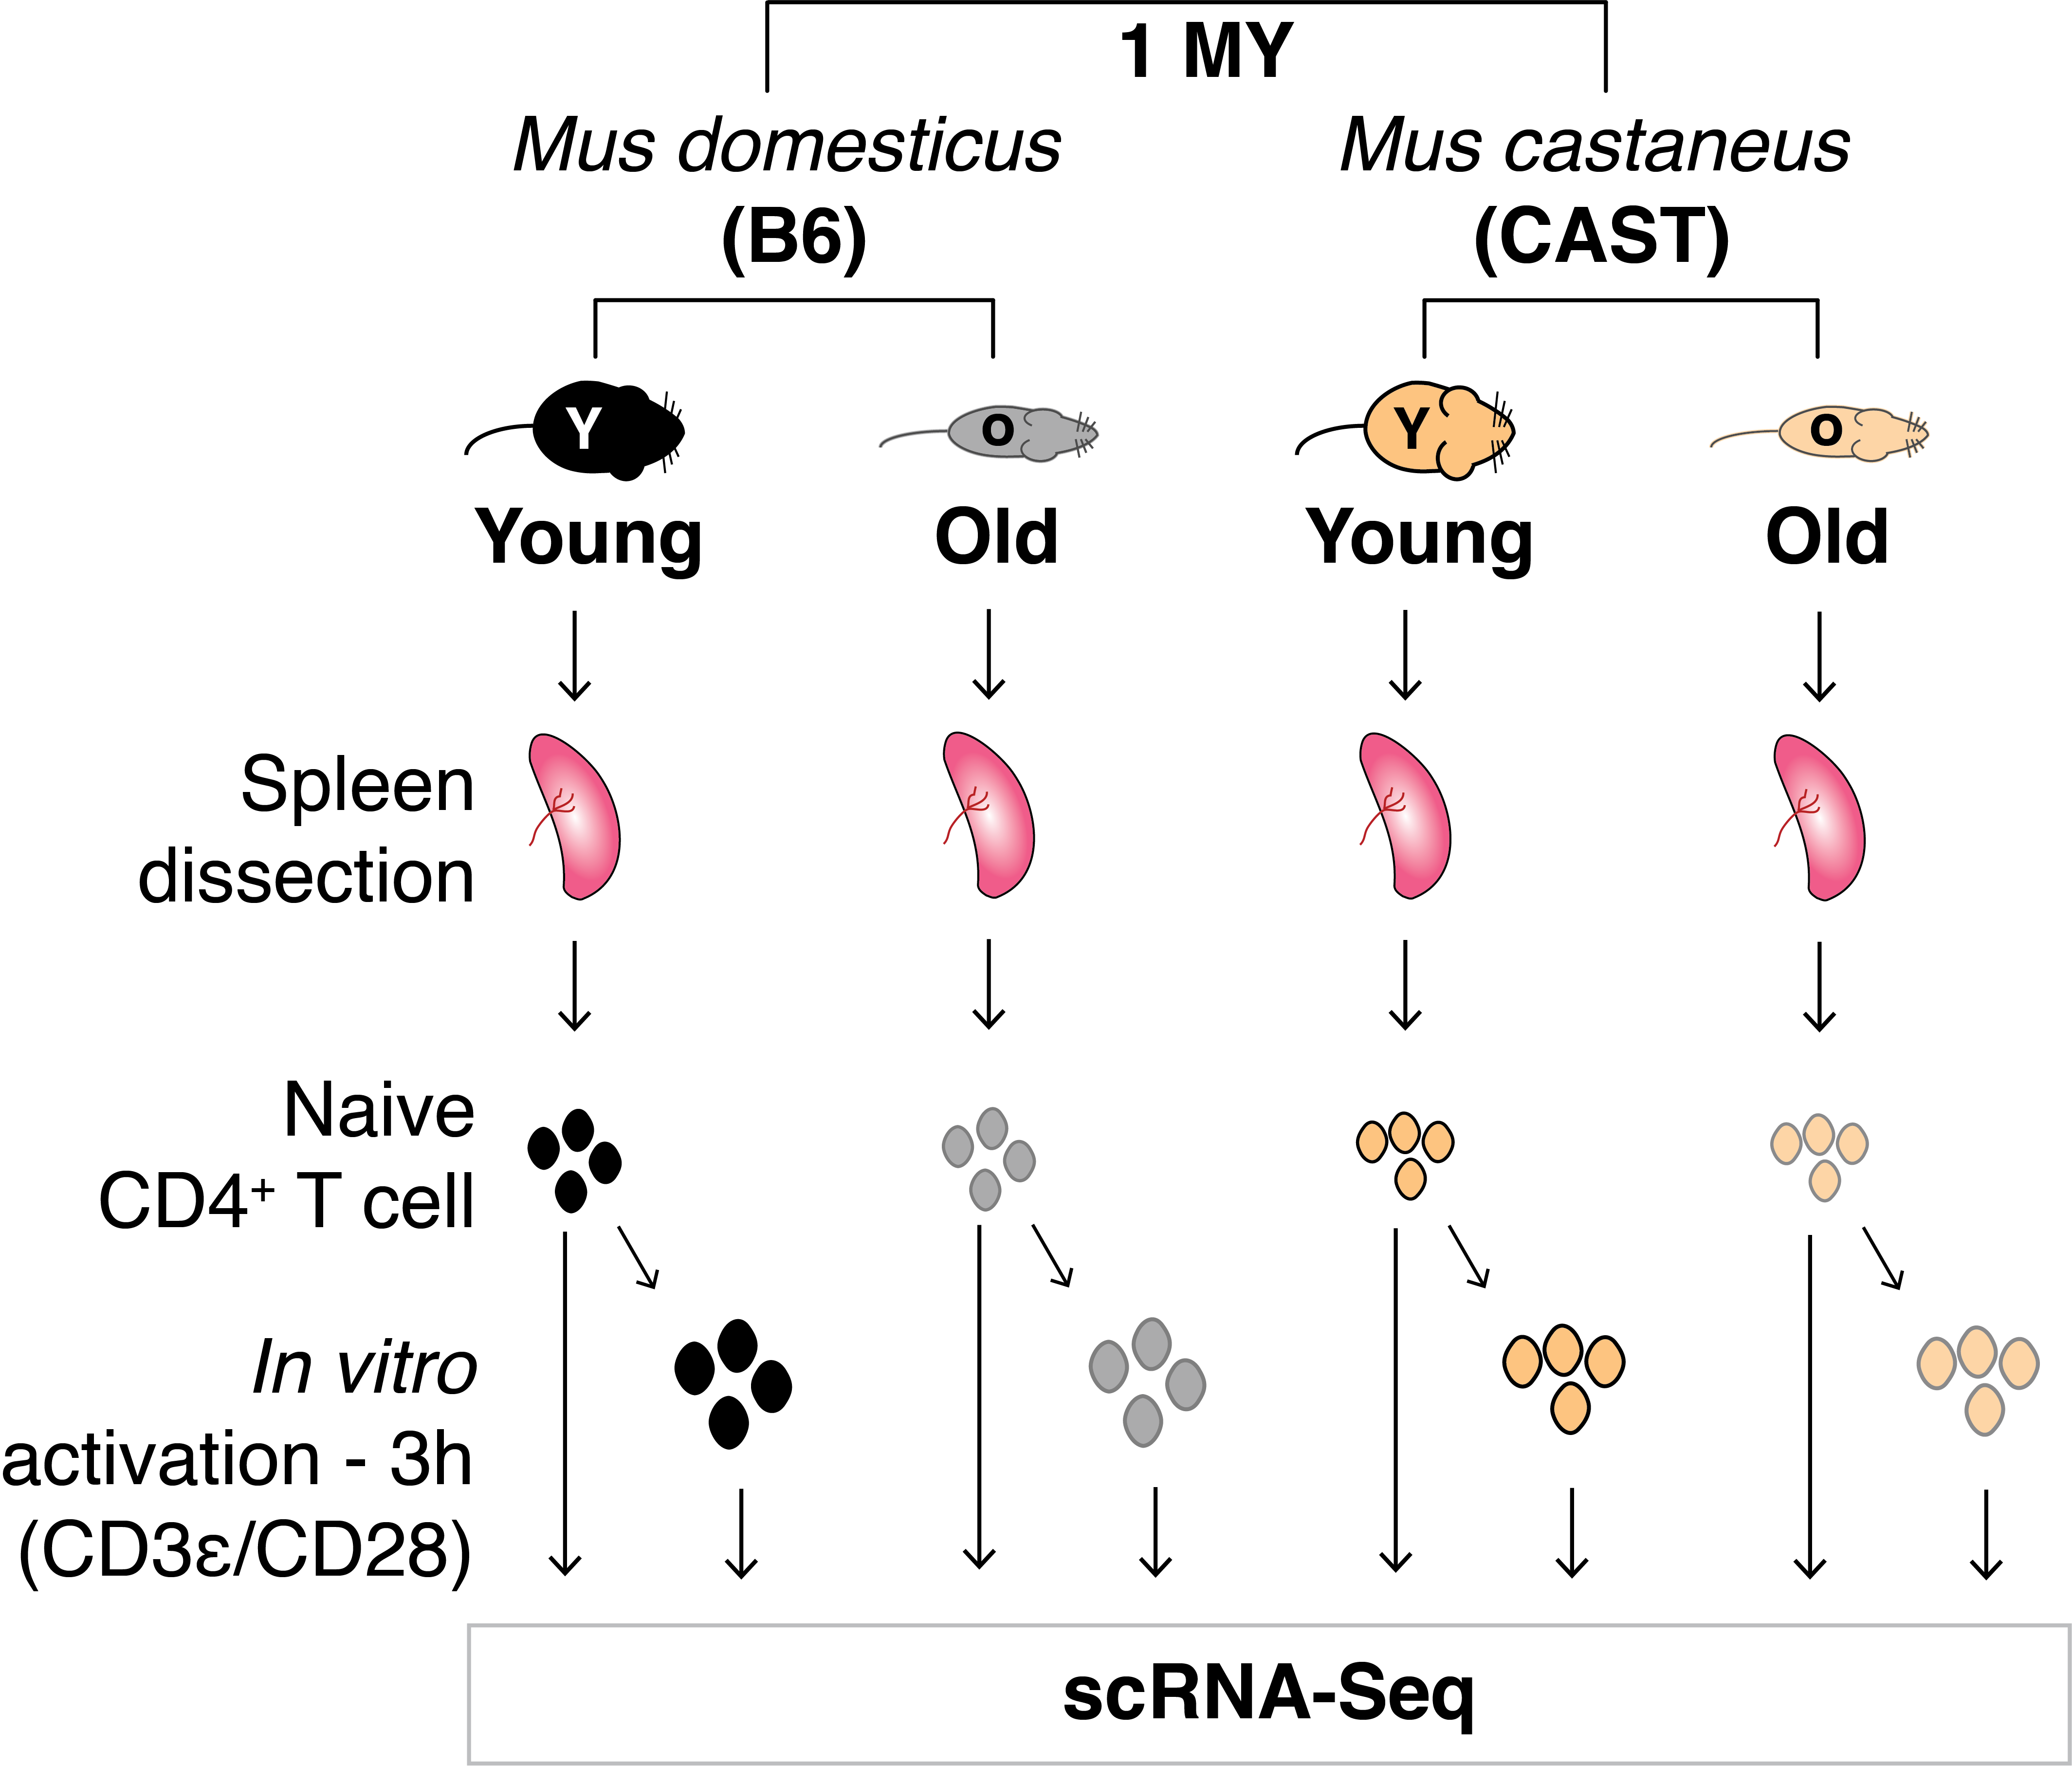
\includegraphics[width=\textwidth]{Fig_1.png}
\caption[Staging of the testicular seminiferous epithelium]{\textbf{Staging of the testicular seminiferous epithelium.}\\
\textbf{(A)} Periodic Acid Schiff (PAS)-stained testis cross-section showing a number of seminiferous tubules at different epithelial stages (displayed as Roman numerals). Within each tubule, the inset circle refers to the corresponding section in (B). Scale bar represents 100 \textmu{}m, \textbf{(B)} Schematic representation of the 12 stages of the seminiferous epithelium in mice. The colour gradient within the circle indicates the differentiation path of germ cells with the layers corresponding to individual cycles of the epithelium. The circle is divided into 12 section, each corresponding to one epithelial stage displaying the characteristic germ cells. Within each section, cells are positioned across the different layers according to their emergence during consecutive cycles, each being 8.6 days apart with more mature cells moving towards the centre, \textbf{(C)} Higher magnification of two tubules depicted in (A). The PAS-stained cross-sections show tubules in Stage VII and Stage X, with the different cell layers indicated by coloured lines. Stage VII tubules contain 4 different layers with germ cells from different generations that are approximately 8.6 days apart, whereas Stage X tubules only contain three layers. Cell types are labelled as: A – type A spermatogonia (SG), In – intermediate SG, B – type B SG, Pl – preleptotene spermatocytes (SCs), L – leptotene SCs, Z – zygotene SCs, P – pachytene SCs, D – diplotene SCs, M – metaphase I and II, 1-8 round spermatids (1-8), 9-16 elongating spermatids (9-16).}
\label{fig3:cell_staging}
\end{figure}

\newpage

To fully elucidate the molecular genetics of germ cell development, it is crucial to sample the full spectrum of germ cells present in testes of adult animals. For this purpose, we employed an unbiased droplet-based scRNA-Seq approach using the 10X Genomics\texttrademark{} platform. 
We used the transcriptomic profiles of thousands of single germ cells to characterize the complex transcriptional dynamics of spermatogenesis at high-resolution. To confidently identify and label cell populations throughout the developmental trajectory, we profiled cells from juvenile testes during the first wave of spermatogenesis. In juveniles, spermatogenesis has only progressed to a defined developmental stage, and therefore allowed us to unambiguously identify the most mature cell type by comparison with adult. The correct labelling of cell types was then used to dissect differentiation processes such as meiosis and spermiogenesis. Furthermore, juvenile samples enriched for spermatogonia which allowed us to characterize spermatogonial differentiation. Another major developmental process during spermatogenesis is the inactivation and reactivation of the X chromosome, which is subject to transcriptional silencing as a consequence of asynapsis \citep{Turner2007}. By combining bulk and single-cell RNA-Seq approaches with chromatin profiling, we identified that \textit{de novo} activated X-linked genes carry distinct chromatin signatures with high levels of repressive H3K9me3 in spermatocytes. \\

Finally, after fully characterising the transcriptional changes during spermatogenesis, I used the regression model presented in the previous chapter to study changes in transcriptional variability over the differentiation time-course. To this end, I generated \emph{post hoc} posterior distribution of linear regression coefficients to statistically test whether individual genes increase or decrease in variability. Furthermore, the clustering of variability profiles showed that rapid transcriptional changes during differentiation can cause peaks in such variability profiles.

\newpage
%!TEX root = ../chapter3.tex
%******************************
%	 Results 
%*****************************

\section{Data generation and processing strategies}

To fully dissect mouse spermatogenesis, we performed three sets of experiments: 1. droplet-based scRNA-Seq of juvenile and adult animals, 2. bulk RNA-Seq of multiple time-points during the first wave of spermatogenesis and 3. CUT\&{}RUN to profile chromatin marks in juvenile mice. The following section will give an overview on the data generation and processing approaches. Detailed analysis steps are explained throughout the chapter. The full experimental set-up can be seen in \textbf{Fig.~\ref{fig3:experimental_design}}.

\begin{figure}[!h]
\centering
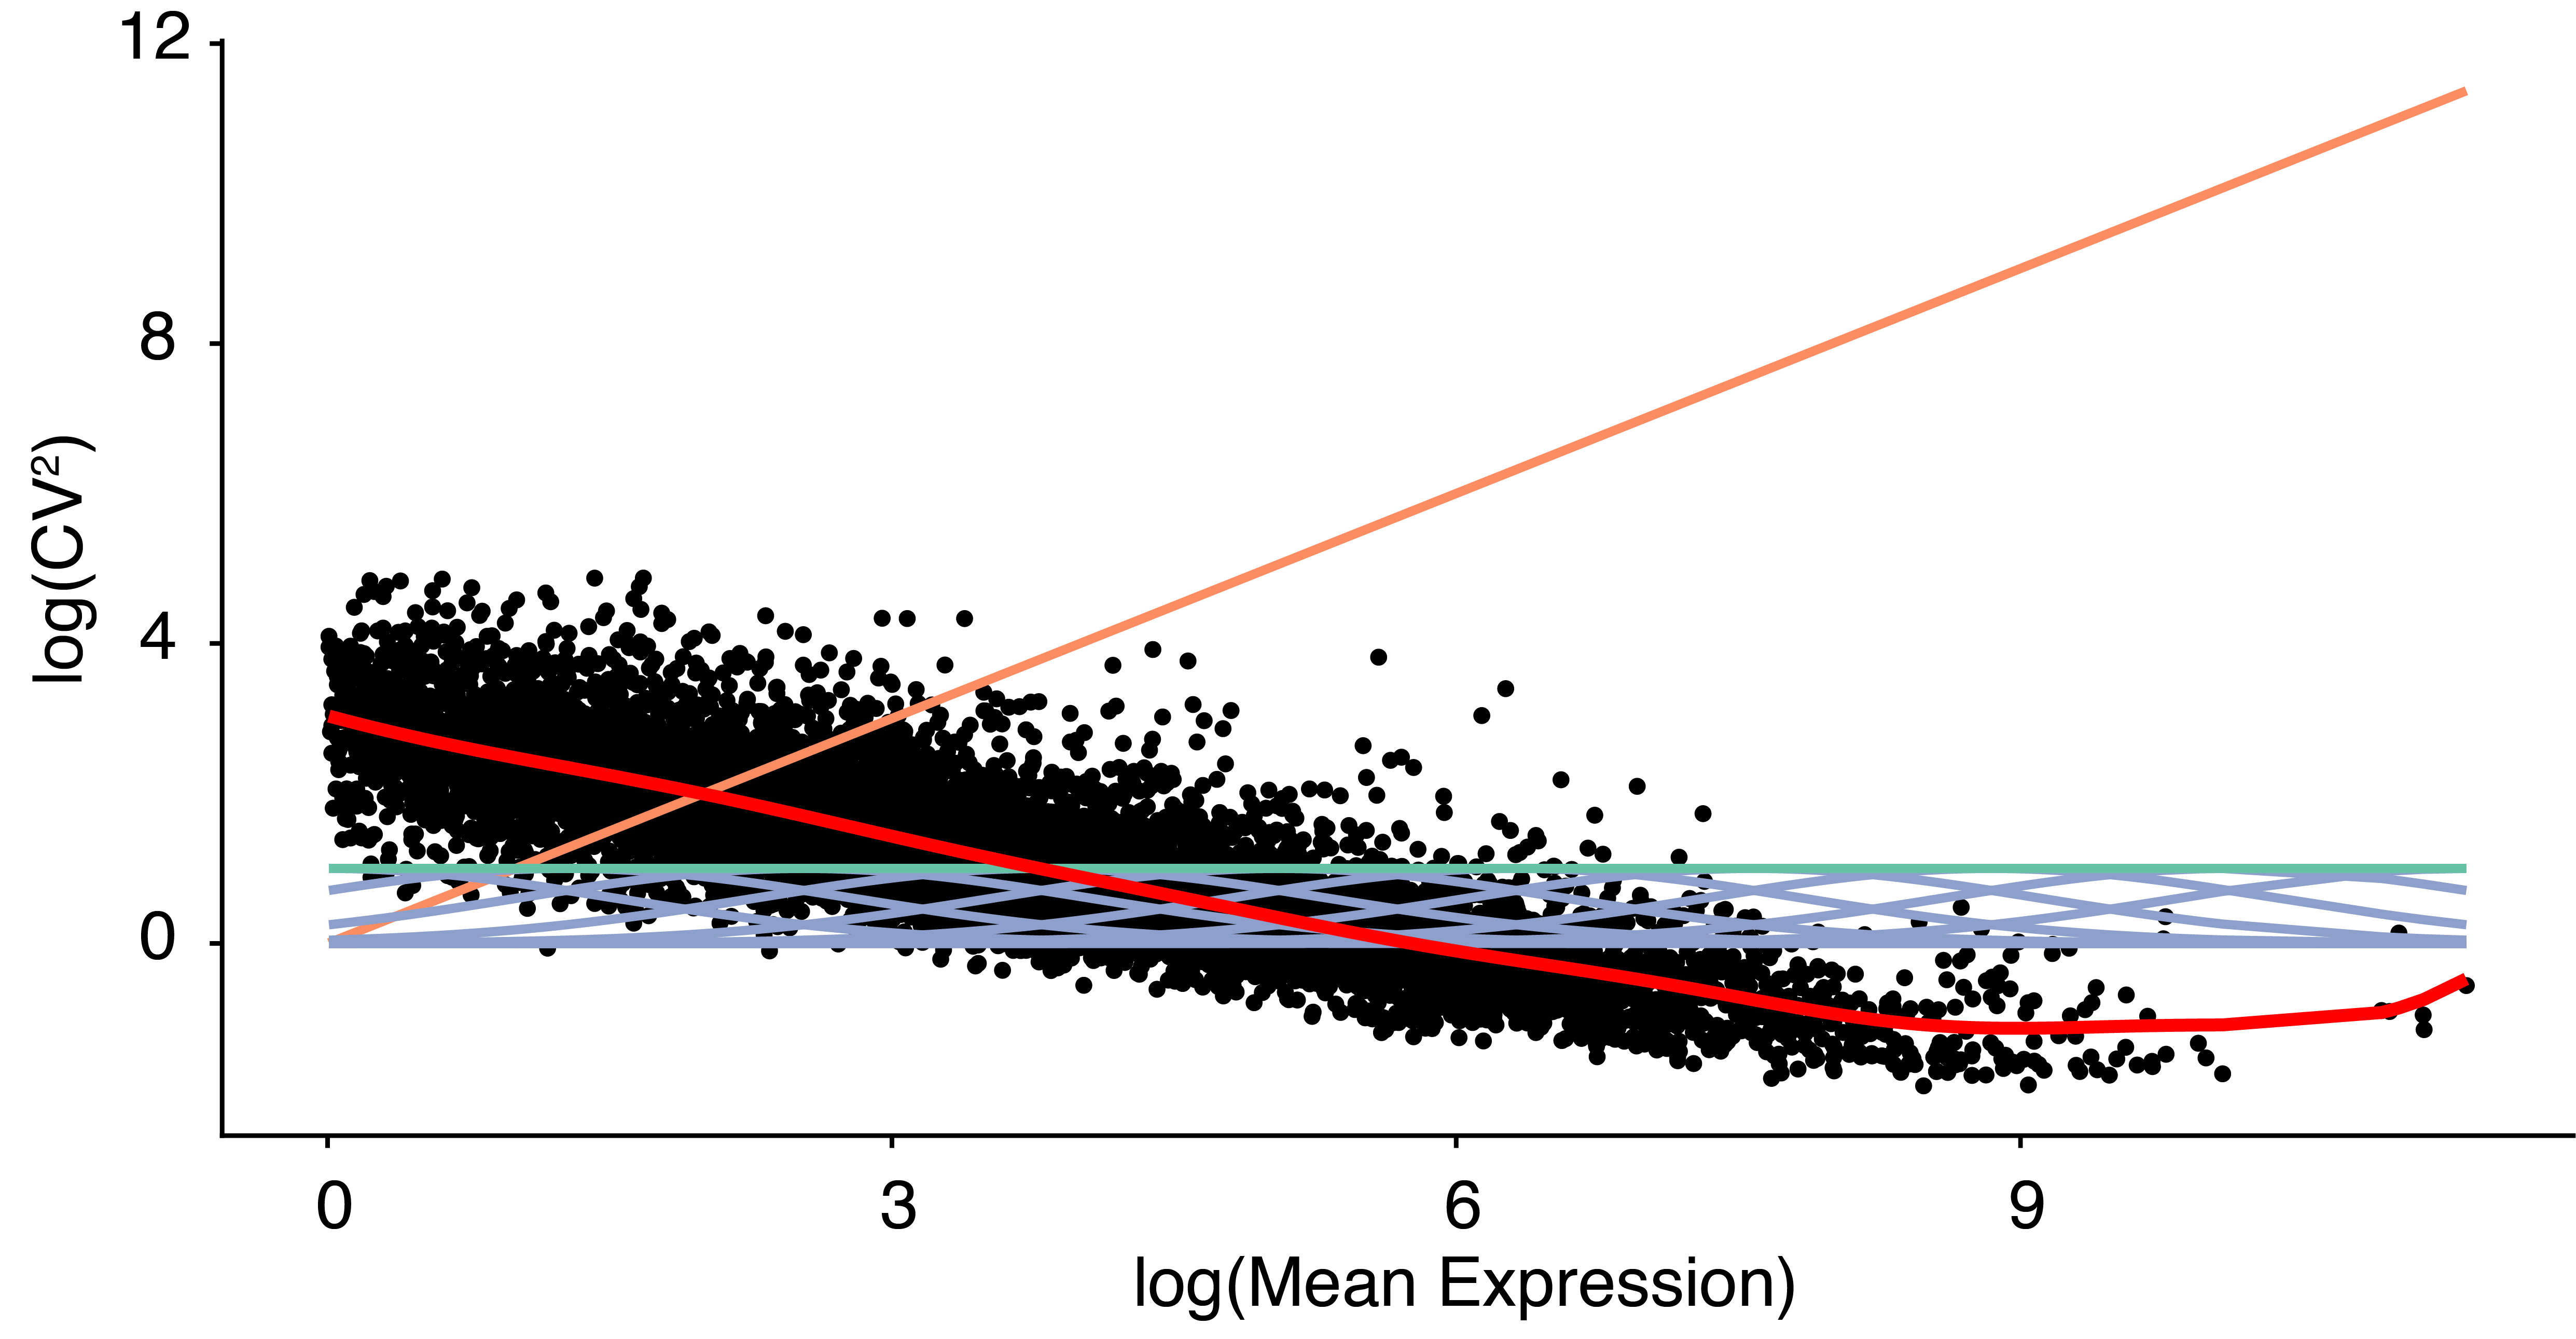
\includegraphics[width=\textwidth]{Fig_2.png}
\caption[Experimental design to dissect mouse spermatogenesis]{\textbf{Experimental design to dissect mouse spermatogenesis.}\\
Overview of the experimental design yielding bulk RNA-Seq, droplet-based scRNA-Seq and chromatin profiling on FACS-purified cells using CUT\&{}RUN from one testis while using the contralateral testis for matched histology.}
\label{fig3:experimental_design}
\end{figure}

\subsection{scRNA-Seq using the 10X Genomics\texttrademark{} system}

Droplet based single-cell RNA sequencing was performed using the 10X Genomics\texttrademark{} technology \citep{Zheng2017}. For this, testes from specifically staged juvenile (between postnatal days 6 and 35) and adult (8-9 weeks) C57BL/6J (B6) mice were dissociated. Single-cell suspensions were loaded into one channel of the 10X Chromium\texttrademark{} Single Cell A Chip, aiming for a recovery of 4000-5000 high-quality cells. Further information on the experimental strategy can be found in \textbf{Appendix \ref{appA.2}} and \textbf{Table \ref{tab3:QC_scRNAseq}} summarises the cells captured per sample.

\newpage

\begin{table}[ht	]
\centering
\caption[Quality filtering of scRNA-Seq data]{\textbf{Quality filtering of scRNA-Seq data.} \\
Quality metrics of droplet-based scRNA-Seq. \textbf{Sample:} Stage information for all samples, \textbf{Library:} sample identifier, \textbf{CellRanger filter:} Number of retained cells after default thresholding using the CellRanger \emph{counts} function,  \textbf{After QC:} Number of cells obtained after quality control (QC), \textbf{Assigned Cell Type:} Number of cells that fall into annotated clusters (removing outlying cells), \textbf{EmptyDrops filter:} Number of cells retained after using the \emph{emptyDrops} function controlling the FDR to 1\%, \textbf{EmptyDrops QC:} Number of cells obtained after quality control (QC) of the \emph{emptyDrops} filtered cells.}
\label{tab3:QC_scRNAseq}
\begin{tabular}{lllllll}
\toprule
\textbf{Sample} & \textbf{Library} & \textbf{CellRanger} & \textbf{After} & \textbf{Assigned} & \textbf{EmptyDrops} & \textbf{EmptyDrops} \\
& & \textbf{filter} & \textbf{QC} & \textbf{Cell Type} & \textbf{filter} & \textbf{QC} \\
\midrule
Adult & do17815 & 1157 & 1157 & 1123 & 4467 & 3400 \\
\midrule
Adult & do17816 & 2198 & 2198 & 2092 & 6145 & 4603 \\
\midrule
P10 & do17821 & 3229 & 3213 & 3212 & 4976 & 4202 \\
\midrule
P15 & do18195 & 4258 & 4258 & 4014 & 14050 & 13168 \\
\midrule
P20 & do17824 & 1775 & 1775 & 1662 & 9400 & 7491 \\
\midrule
P25 & do18196 & 4334 & 4334 & 4130 & 8038 & 6802 \\
\midrule
P30 & do17825 & 2278 & 2278 & 2211 & 5393 & 4958 \\
\midrule
P35 & do17827 & 3160 & 3160 & 3004 & 49002 & 10683 \\                 
\bottomrule   
\end{tabular}
\end{table}

To process droplet-based scRNA-Seq data after sequencing, 10X genomics\texttrademark{} developed a set of processing pipelines termed \textit{Cell Ranger}. We obtained gene-specific transcript counts using the Cell Ranger \emph{count} function with default settings. This pipeline aligns reads against the \emph{Mus musculus} genome (GRCm38) and counts UMIs per transcript and sample. This software retains cells with similar UMI distributions \citep{Zheng2017}. We use this default threshold to obtain high-quality cells with large numbers of UMIs. For further quality control and after merging cells of all samples, we filtered out cells that express less than 1000 genes. Additionally, we exclude cells with more than 10\% of reads mapping to the mitochondrial genome. The number of remaining cells per sample can be seen in \textbf{Table \ref{tab3:QC_scRNAseq}}.\\

The Cell Ranger \emph{count} pipeline performs thresholding on the number of UMIs per cell to exclude empty droplets or droplets with low-quality cells. This default threshold excludes smaller cells with lower transcriptional complexity form a mixture containing cells with broadly different transcriptional complexities. We therefore used the \emph{emptyDrops} function provided in the \emph{DropletUtils} Bioconductor package to statistically distinguish empty droplets from genuine cells (controlling the FDR to 1\%) \citep{Lun2018}. Nevertheless, further quality control needs to be performed and after merging all remaining cells across all samples, we filtered out cells with less than 500 genes expressed. Furthermore, we excluded cells with more than 10\% or mitochondrial genes expressed \textbf{(Table \ref{tab3:QC_scRNAseq})}.\\
 
The transcriptomes of quality filtered cells were normalized using the \emph{scran} package \citep{Lun2016pooling}. For this, cells with similar transcriptomic complexity were pre-clustered using a graph-based approach (as implemented in the \emph{quickCluster} function). Size factors were
calculated within each cluster before being scaled between clusters using the \emph{computeSumFactors} function. Throughout this paper, the log$_2$-transformed, normalized counts (after adding one pseudocount) are displayed. For down-stream analysis, lowly expressed genes (averaged log$_2$-transformed, normalized expression < 0.1) were excluded. After quality control and filtering, we retained more than 20,000 high-quality single cells and over 46,000 cells including the once with lower transcriptional complexity \textbf{(Table \ref{tab3:QC_scRNAseq})}. These cells were used to dissect molecular processes during spermatogenesis and to profile under-represented and transcriptionally inactive cell types in mouse testes. 

\subsection{Bulk RNA-Seg from juvenile animals}

Additionally, we generated whole-tissue bulk RNA-Seq libraries from time-points during the first wave of spermatogenesis (\textbf{Appendix \ref{appA.2.bulk}}). More specifically, we sampled (in replicates) testes from mice at post-natal (P) day P6 (2x), P8, P10 (2x), P12 (2x), P14 (2x), P16, P18 (2x), P20 (2x), P22 (2x), P24 (2x), P26 (2x), P28 (2x), P30 (2x), P32, P34, P35 and from adult animals (2x). Detailed experimental methods can be found in \textbf{Appendix \ref{appA.2.bulk}}. 
Sequencing reads were aligned against the \textit{Mus musculus} genome (GRCm38) using the \emph{STAR} aligner with default settings \citep{Dobin2013}. \\

Gene-level transcript counts were obtained using \emph{HTSeq} \citep{Anders2014} with the –s option set to “reverse” and using the GRCm38.88 genomic annotation file. We visualized several features of the aligned and counted data (number of intronic/exonic reads, number of multi-mapping reads, low-quality reads and total library size) and did not detect any low-quality RNA-Seq libraries. Next, we used the size factor normalization approach implemented in DESeq2 \citep{Love2014} for data normalization. For down-stream analysis and visualization, lowly expressed genes (averaged counts < 10) were excluded. With this, we generated 30 bulk RNA-Seq libraries that will be used for developmental staging of cell types and the dissect X chromosome expression dynamics.

\subsection{CUT\&{}RUN from juvenile animals}

To map chromatin states in purified cell populations we used CUT\&{}RUN (Cleavage Under Targets \& Release Using Nuclease) \citep{Skene2018}. Detailed experimental methods can be found in \textbf{Appendix \ref{appA.2.CnR}}. In brief, spermatocytes and spermatids were sorted as described in \textbf{Appendix \ref{appA.2.sorting}} and attached to concanavalin A–coated magnetic beads. After permeabilisation, anti-bodies against H3K9me3 and H3K4me3 were incubated with the cells. Inactive micrococcal nuclease linked to protein A was added to the mix and cooled to 0$^\circ$. Protein A binds to the antibodies and upon activation the nuclease digests DNA next to the histones where the antibody bound. Cleaved DNA fragments diffused out of the nucleus and were prepared for sequencing. This technique allows targeted chromatin profiling for specific marks at a genome wide level and requires minimal cell input \citep{Skene2018}.\\

Sequencing reads were aligned to the Mus musculus genome (GRCm38) using \textit{Bowtie2} with the following settings: --local --very-sensitive-local --no-unal -q --phred33. Paired end reads were counted in specified regions using the \textit{regionCounts} function implemented in the \textit{csaw} Bioconductor package \citep{Lun2015}. For this, duplicated reads, reads mapped more than 1000 bp apart and reads mapping to blacklisted regions (available at: \url{http://mitra.stanford.edu/kundaje/akundaje/release/blacklists/mm10-mouse/mm10.blacklist.bed.gz}) were removed. Regions of interests were: promoters (obtained using the \textit{promoters} function of the \textit{GenomicFeatures} package), 1000 bp windows across the chromosome (using the \textit{windowCounts} function of \textit{csaw}) and whole chromosomes. Counts per region were normalized based on library size (counts per million, CPM) for promoter regions and 1000 bp windows. Additionally, when considering entire chromosomes, the length of the chromosome was accounted for by computing the Fragments per Kilobase per Million mapped reads (FPKMs). 

\newpage

\subsection{Identification of germ cell-types across all scRNA-Seq samples}
\label{sec3:clustering}

After data generation and pre-processing steps, we next characterized the detectable cell-types across all scRNA-Seq samples. We assume that cell-types sampled from juvenile animals are also found among the cell types sampled from adult animals. To detect cell-types consistently across all scRNA-Seq samples, we first performed batch correction. To remove batch-specific effects that arise when samples are prepared and sequenced in different experiments \textbf{(Tables \ref{tab3:QC_scRNAseq})}, we used the \emph{mnnCorrect} function implemented in the \emph{scran} package \citep{Haghverdi2018}. We used the top 1000 genes with highest biological variation across all samples as informative genes for batch correction. The \emph{mnnCorrect} function takes transcriptional profiles of cells isolated from adult B6 mice as first input and uses this dataset as reference for cell mapping. This approach maps the juvenile samples onto the adult B6 \textbf{(Fig.~\ref{fig3:cell_types}A)}.\\

To identify cell types across all samples, batch corrected transcriptomes were clustered using a graph-based approach. A shared nearest-neighbour (SNN) graph \citep{Xu2015} was constructed considering 3 shared nearest neighbours using the \emph{buildSNNGraph} function in \emph{scran}. In the next step, a multi-level modularity optimization algorithm was used to find community structure in the graph \citep{Blondel2008} implemented in \emph{igraph} R package. Cells in small clusters that show unclear identities were excluded from down-stream analysis. In total, we identified 28 cluster. To correctly label cell clusters based on their cell-type, we identified marker genes for all germ cell-types in the adult B6 samples. To this end, we performed differential expression testing using multiple pairwise comparisons. To detect cluster-specific marker genes, the \emph{findMarkers} function implemented in \emph{scran} was used on the log$_2$-transformed normalized counts while providing the cluster labels \textbf{(Fig.~\ref{fig3:cell_types}B)}. \\

On a broad level and by visualizing the expression of detected marker genes, we identified the following cell types: spermatogonia (based on \textit{Dmrt1} expression, \citep{Matson2010}), spermatocytes (\textit{Piwil1}, \citep{Deng2002}), round and elongating spermatids (\textit{Tex21} and \textit{Tnp1}, respectively, \citep{Fujii2002}), as well as the main somatic cell types of the testis, Sertoli (\textit{Cldn11}, \citep{Mazaud-Guittot2010}) and Leydig cells (\textit{Fabp3}, \citep{Oresti2013}) \textbf{(Fig.~\ref{fig3:cell_types}B)}. Using a dimensionality reduction technique for visualization (t-distributed Stochastic Neighbour Embedding; \textbf{Fig.~\ref{fig3:cell_types}C}), the germ cell types from spermatocytes to elongating spermatids formed a continuum, which recapitulated the known developmental trajectory.

\newpage

\begin{figure}[!h]
\centering
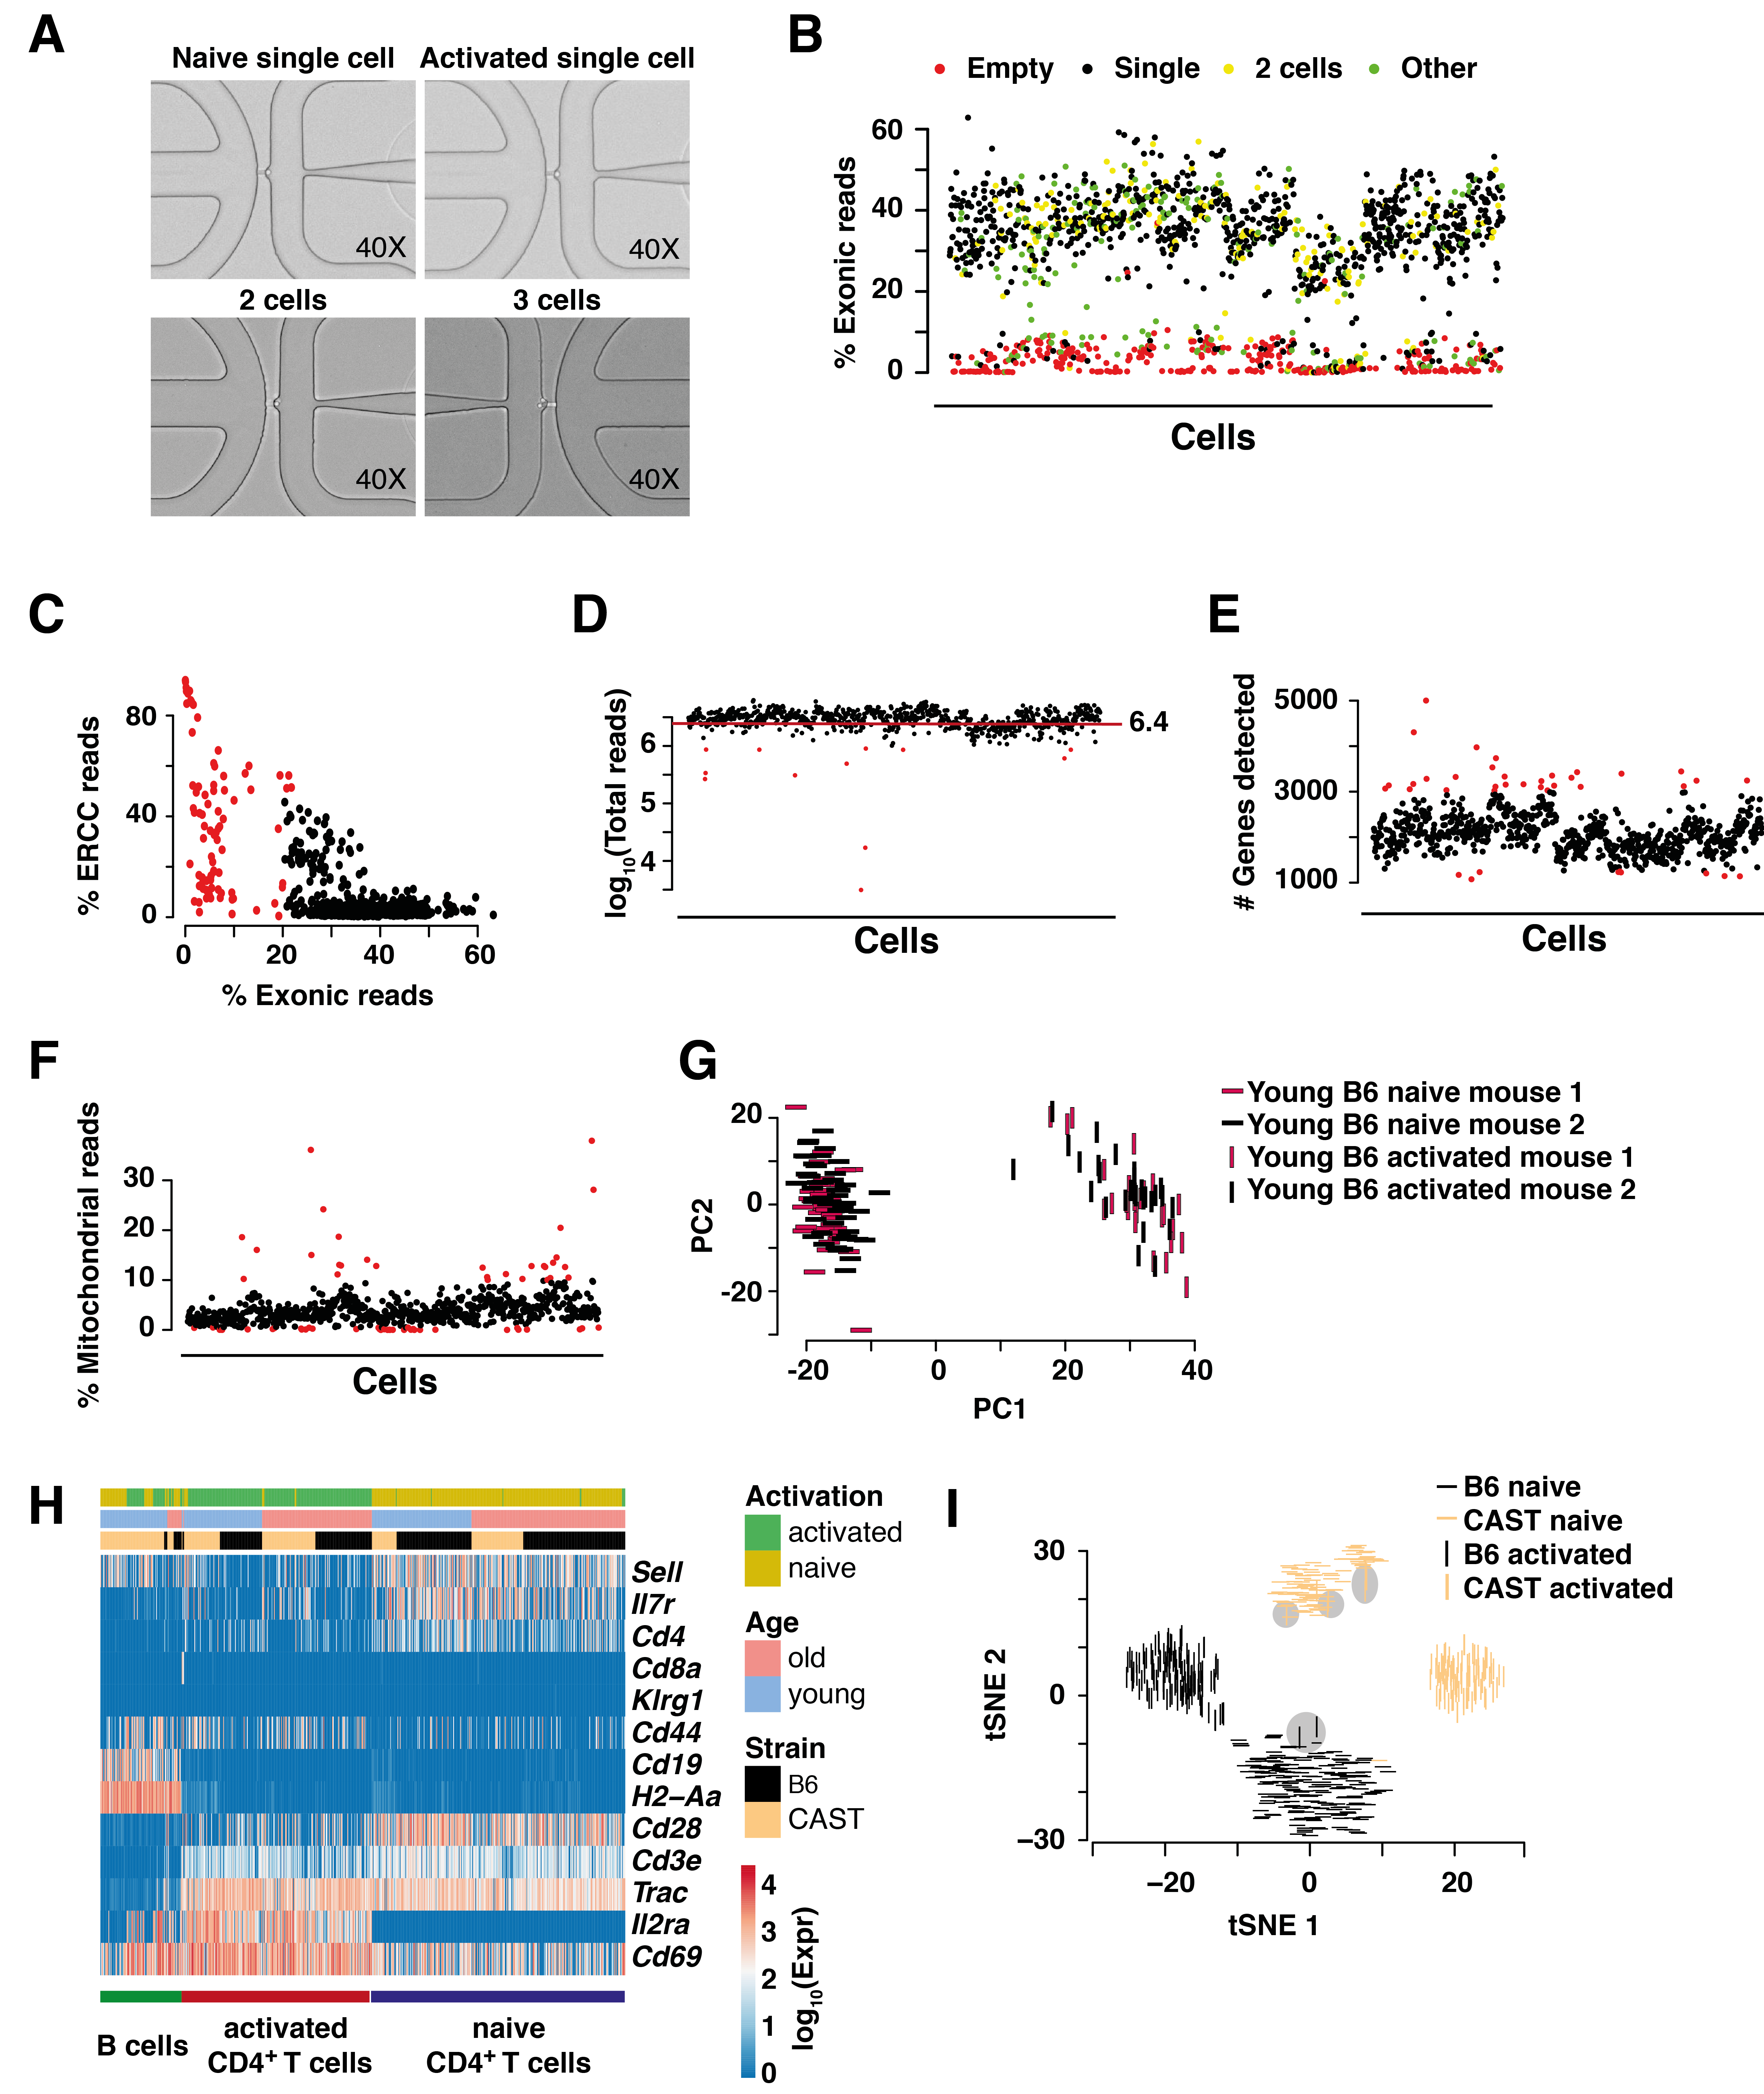
\includegraphics[width=\textwidth]{Fig_3.png}
\caption[Droplet based scRNA-Seq of juvenile and adult mouse spermatogenesis]{\textbf{Droplet based scRNA-Seq of juvenile and adult mouse spermatogenesis.}\\
\textbf{(A)} tSNE representation of juvenile cells that were mapped to cells isolated from adult mice. Grey dots indicate all cells from adult animals that were used as a reference for cell mapping. Coloured dots represent cells isolated at each sampled stage during the first wave of spermatogenesis. Clustering has been perfomed across all cells after cell mapping. SG: Spermatogonia, M: Metaphase, IL: Imature Leydig, PTM: Peritubular Myoid Cells, EC: Endothelial Cells, tMg: testicular Marcophages, \textbf{(B)} tSNE representation of scRNA-Seq data from adult B6 mice with the colour gradient representing the expression of known marker genes for two somatic cell types and the main germ cell types. The x- and y-axis represent the first and second dimension of tSNE respectively. The colour legend shows log$_2$-transformed, normalized expression counts, \textbf{(C)} Graph-based clustering identifies different sub-stages within major germ cell populations form adult B6 animals. 
}
\label{fig3:cell_types}
\end{figure}

\newpage

\section{Developmental staging of mouse spermatogenesis}

Historically, sub-staging of the major cell types within the testis was based on changes in nuclear or cellular morphology \citep{Oakberg1956,  Oakberg1956a}. Previous attempts to complement morphology with molecular signatures have been limited to FACS-based and sedimentation assays, where the resolution was unable to differentiate between sub-cell-types \citep{Bastos2005, Gaysinskaya2014, Lam1970, Meistrich1977, Romrell1976, Soumillon2013}. While a mixture of all spermatogenic cell types co-exists in the adult, the first wave of spermatogenesis during juvenile development is more synchronised. Starting around mouse postnatal day P4, spermatogonia begin to differentiate, forming the first generation of spermatocytes as early as P10, round spermatids by P20, and completing the first wave of spermatogenesis with the production of mature spermatozoa between P30 and P35 \textbf{(Fig.~\ref{fig3:cell_staging}B and \ref{fig3:1st_wave}A)} \citep{Bellve1977, Janca1986, Nebel1961}. In this section, we define well-known developmental transitions during spermatogenesis by (i) mapping cells sampled from defined epithelial stages during the first wave of spermatogenesis to cells sampled from adult testes and (ii) classifying the cell-types identified above using bulk RNA-Seq sampled from juvenile testes every two days during the first wave of spermatogenesis. 

\subsection{Cell type characterization using the first wave of spermatogenesis}
 
We exploited the synchronised development of cell types throughout the first wave of spermatogenesis to define major and morphologically described check-points of the differentiation process. For this, we sampled multiple time-points from juvenile animals to identify the most mature (differentiated) cell types. At any given time-point during the first wave of spermatogenesis, there exist a defined number of known cell types in juvenile testis depending on the timing of the developmental cycle \textbf{(Fig.~\ref{fig3:cell_staging}B)}. Based on known sperm developmental transitions, we chose six time points between P10 and P35 from which to generate single-cell RNA-Seq libraries \textbf{(Fig.~\ref{fig3:1st_wave}A and Table \ref{tab3:QC_scRNAseq})}. As described above, we mapped the transcriptomes of juvenile samples onto the adult B6 sample \textbf{(Fig.~\ref{fig3:cell_types}A)}. For each juvenile experiment, we found that the population of developing germ cells was strongly enriched at the expected developmental stage, as quantified by the percentage of cells in each cell-type cluster \textbf{(Fig.~\ref{fig3:1st_wave}C)}. By associating the known cell-types from juvenile animals with the corresponding cell types in the adult trajectory, we unambiguously assigned molecular and histological signatures to cells during adult spermatogenesis.

\newpage

\begin{figure}[!h]
\centering
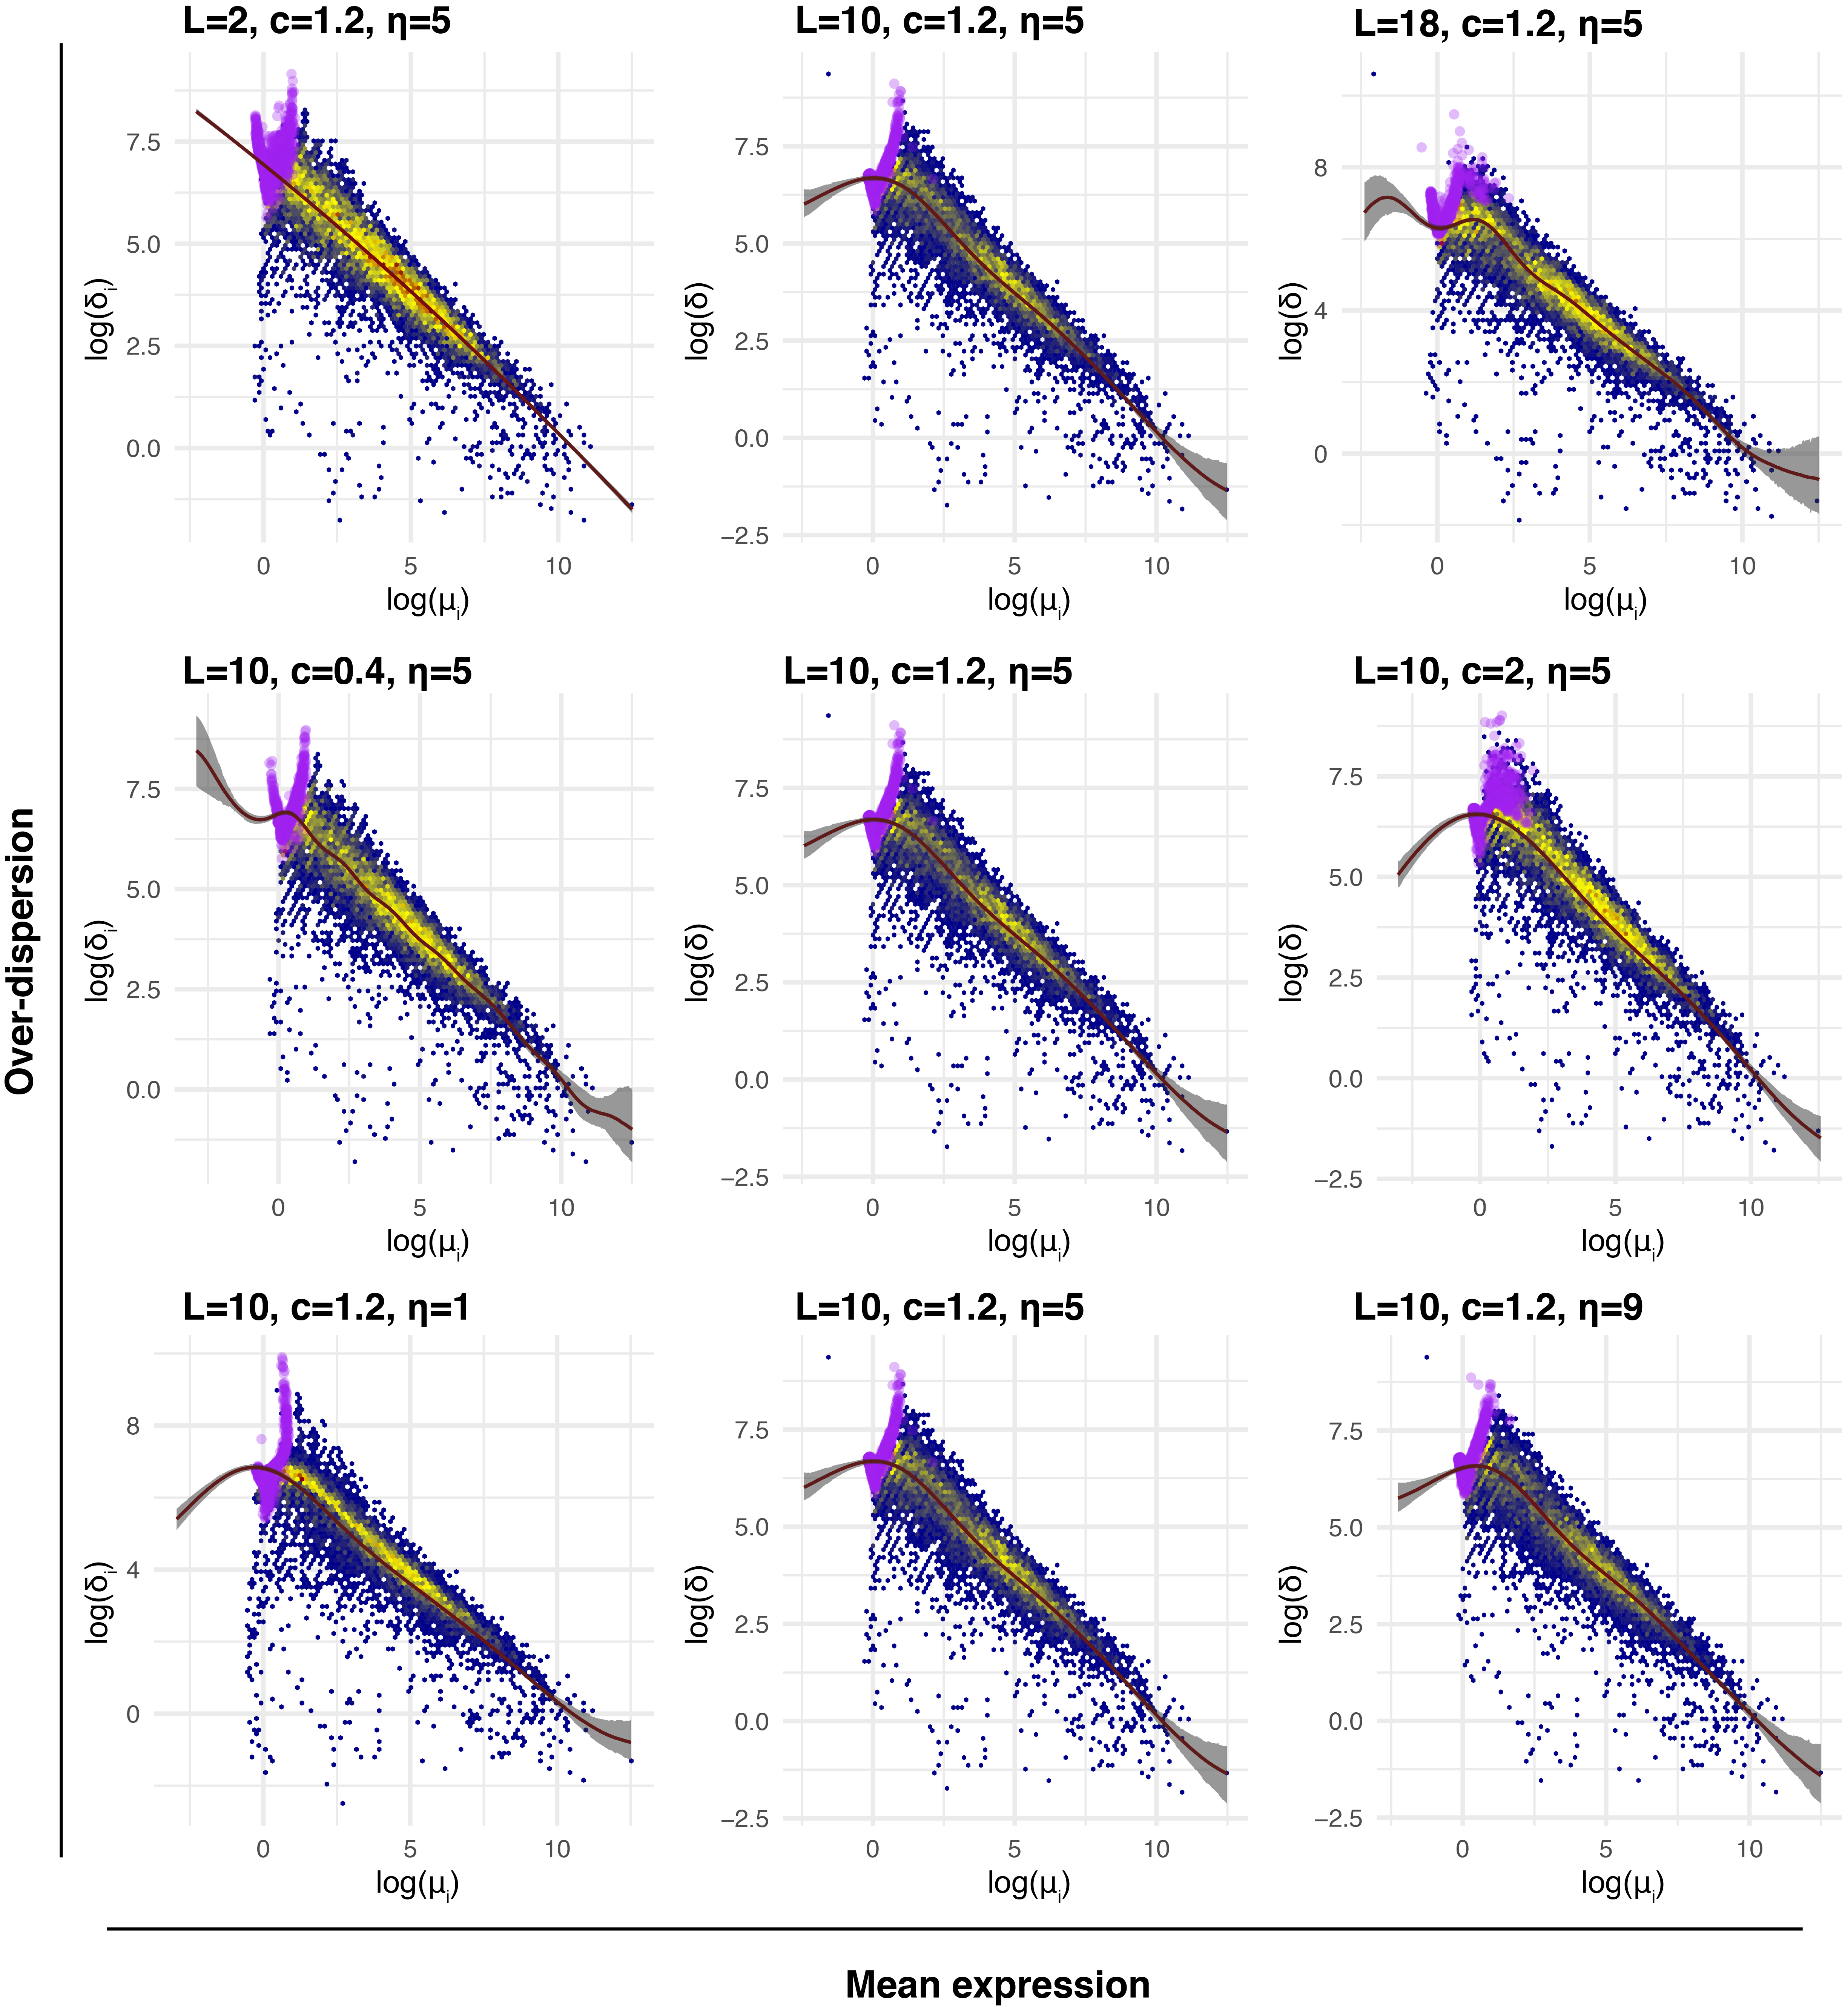
\includegraphics[width=0.95\textwidth]{Fig_4.png}
\caption[Staging of cell types during mouse spermatogenesis]{\textbf{Staging of cell types during mouse spermatogenesis (full legend on next page).}}
\label{fig3:1st_wave}
\end{figure}

\newpage

\captionsetup[figure]{list=no}
\addtocounter{figure}{-1}   
\captionof{figure}{\textbf{Staging of cell types during mouse spermatogenesis (continued).}\\
\textbf{(A)} Schematic representation of the major germ cell types and their corresponding developmental processes. Spermatogonia differentiate undergoing mitotic cell divisions before forming spermatocytes that divide by meiotic division. Following meiosis, spermatids differentiate throughout spermiogenesis to form mature sperm. The timeline in the lower panel indicates at which point during the first wave of spermatogenesis samples were harvested for the generation of scRNA-Seq (X) or bulk RNA-Seq (B) data, \textbf{(B)} Representative images of seminiferous tubules from animals harvested at different postnatal (P) time points during the first wave of spermatogenesis. The approximate timing of the stage and cycle of the tubule is illustrated below in the form of a circle (see Fig.~\ref{fig3:cell_staging}B), \textbf{(C)} After cell mapping and clustering, the percentage of cells in each cluster can be calculated for each sample. The size of squares corresponds to this percentage and the colours indicate the cluster labels depicted in Fig.~\ref{fig3:cell_types}C. tSNEs on the right-hand side of each panel (juvenile samples only) illustrate progress through spermatogenesis. SG: spermatogonia, M: metaphase, \textbf{(D)} Probabilistic mapping of bulk RNA-Seq libraries to the cell clusters identified in the adult scRNA-Seq data using a random forest approach. The colour gradient indicates the probability with which a bulk sample can be assigned to the specific cell cluster.  \\}
\captionsetup[figure]{list=yes}

In adult, we detect a homogeneous distribution of cells across the germ cell types ranging from spermatogonia to S14 spermatids \textbf{(Fig.~\ref{fig3:1st_wave}C)}. To characterize germ cell-types, we focused on samples taken from P15-P35 animals since at P10 the majority of cell types do not show germ cell properties \textbf{(Fig.~\ref{fig3:cell_types}A)}. In earlier stages, cells are enriched the most mature cell-type in each cycle. For instance, at P15 the majority of cells are spermatogonia and spermatocytes progressing through the mid-pachytene stage \citep{Turner2004}. Interestingly, less mature cells-types that exists earlier to mid-pachytene cells are also present at this time point (and later time points). This supports recent reports that the first wave of spermatogenesis is less synchronized than previously anticipated \citep{Snyder2010}. At P20, we detect an enrichment for spermatocytes, cells undergoing meiotic cell division, and a small group of early round spermatids. This population structure is in line with matched histology, which shows a large number of tubules in late stages IX-XII and the first occurrence of early round spermatids \citep{Bellve1977}. It has been shown that spermatids first reach the elongating state, which occurs from S10 spermatids onwards, between P24 and P26 \citep{Janca1986}. At P25, we observed that cells mapped to our first ten clusters of spermatids, which we then labelled according to morphologically-defined spermatid substages S1 – S10 \textbf{(Fig.~\ref{fig3:1st_wave}C)}. At P30 and P35, we observed a relatively even distribution of cells across all groups, closely resembling the adult distribution up to S14, indicating that the first wave of spermatogenesis is complete. With this computational mapping of cells collected at different developmental time-points, we linked transcriptional profiles of single cells to, morphologically defined transitions during germ cell development.

\newpage

\subsection{Classification of cell types based on bulk RNA-Seq data}

While the analysis performed above only determines crucial developmental transitions during spermatogenesis, we did not achieve high-resolution for the developmental mapping of defined cell-types to the clusters identified above. To further validate the identity of the cell clusters, we used bulk RNA-Seq from testis collected during the first wave of spermatogenesis. These samples were harvested every two days between P6 and P34 and allow us to refine the mapping analysis performed above \textbf{(Fig.~\ref{fig3:1st_wave}A)}. The batch-correction approach used above was developed to match hundreds of single cells across samples and is therefore not suitable to map the 30 bulk RNA-Seq samples onto the adult trajectory. To classify each bulk RNA-Seq sample to one or multiple clusters identified in the scRNA-Seq data, we used a regression approach that performs probabilistic classification. Using the top 50 cluster-specific marker genes for spermatogonia, all spermatocyte groups, all spermatid groups, sertoli and leydig cells, we trained a random forest classifier (implemented in the \emph{randomForest} R package \citep{Liaw2002}) on 2000 cells isolated from adult B6 testes. Model testing was performed on the remaining 1215 cells isolated from adult B6 testes. Prior to training and testing, log$_2$-transformed, normalized counts were scaled by computing the Z score for each gene. Probabilistic prediction was performed using the Z score of log$_2$-transformed, normalized bulk RNA-Seq reads of the input genes. The output of this analysis is the classification probability for each bulk RNA-Seq sample to belong to each scRNA-Seq cluster.\\

This classification confirmed that between P6 – P14 spermatogonia and somatic cells show the highest contribution to the transcriptomic profile \textbf{(Fig.~\ref{fig3:1st_wave}D)}. Between P16 and P20 we observed the emergence of spermatocyte-specific gene expression signatures, after which spermatids become the transcriptionally dominant cell type. By P26, spermatids reach the elongating state where transcription is uniformly shut-down due to the beginning of the histone-to-protamine transition \citep{Steger1999}. Following this, changes in RNA content are mostly due to degradation. Bulk transcriptional profiles can only be classified up to S10 because transcription is largely inactive thereafter and no new cluster-specific marker genes emerge.  

\newpage

\section{Under-represented cell types in spermatogenesis}

The analysis of early stages of juvenile mice in the previous section showed an enrichment for cell-types that are relatively under-represented in later stages and in adult (e.g.~spermatogonia and early spermatocytes at P15, \textbf{Fig.~\ref{fig3:1st_wave}C}). Additionally, we detected the absence of germ cells in the P10 sample which leads to a relative enrichment of somatic cell types present in mouse testes \textbf{(Fig.~\ref{fig3:cell_types}A)}. This relative enrichment allows us to dissect somatic cell types and spermatogonial differentiation at higher resolution compared to cells isolated from adult samples.

\subsection{Somatic cell types in juvenile testes}

To study heterogeneity within the somatic cell population, we focused on the P10 stage, where somatic cells are relatively more frequent \textbf{(Fig.~\ref{fig3:somatic_cells})}. As expected, we identify substantial numbers of Sertoli and Leydig cells, which are the main somatic cell types in adult. Leydig cells are the primary major producers of steroid hormones such as testosterone that regulate sexual differentiation and development of secondary sex characteristics \citep{Svechnikov2010, Haider2004}. Sertoli cells on the other hand reside inside the tubules and provide structural features for testis development. They further support differentiating germ cells by providing growth factors and nutrients  \citep{Griswold1998}. In addition, we newly identified a large population of immature (fetal) Leydig cells (IL), based on \textit{Dlk1} expression \citep{Lottrup2014}. ILs shape the embryonic development of testes and rapidly decline in numbers after birth \citep{Griswold2009}. \\

Furthermore, we detected the cells that form the basal lamina. These include peritubular myoid cells (PTM, \textit{Acta2}, \citep{Cool2008}), vascular endothelial cells (\textit{Tm4sf1}, \citep{Shih2009}), and testicular macrophages (\textit{Cd14}, \citep{Kitchens2000}) \textbf{(Fig.~\ref{fig3:somatic_cells}A and B)}. PTM are contractile cells that form the wall of seminiferous tubules and induce the release of the testicular fluid which contains mature spermatozoa \citep{Diez-Torre2011}. In addition, endothelial cells play a major role in forming the testis cord during development and together with PTMs surround sertoli cells in the adult testes \citep{Combes2009}. Testicular macrophages are the most abundant immune cell type in the organ and play a crucial role in testes development by expressing anti-inflammatory cytokines that induce a tolerogenic environment in testes. This is needed since germ cell specific antigens are only expressed after puberty when the immune system has already matured \citep{Fijak2006}. By performing differential expression analysis (using the \emph{findMarkers} function in \emph{scran}), we identified novel markers for these cell populations that are relatively under-represented in adult testes. \textbf{Fig.~\ref{fig3:somatic_cells}B} visualises the top marker genes for the enriched somatic cell types detected at P10.\\

\begin{figure}[!h]
\centering
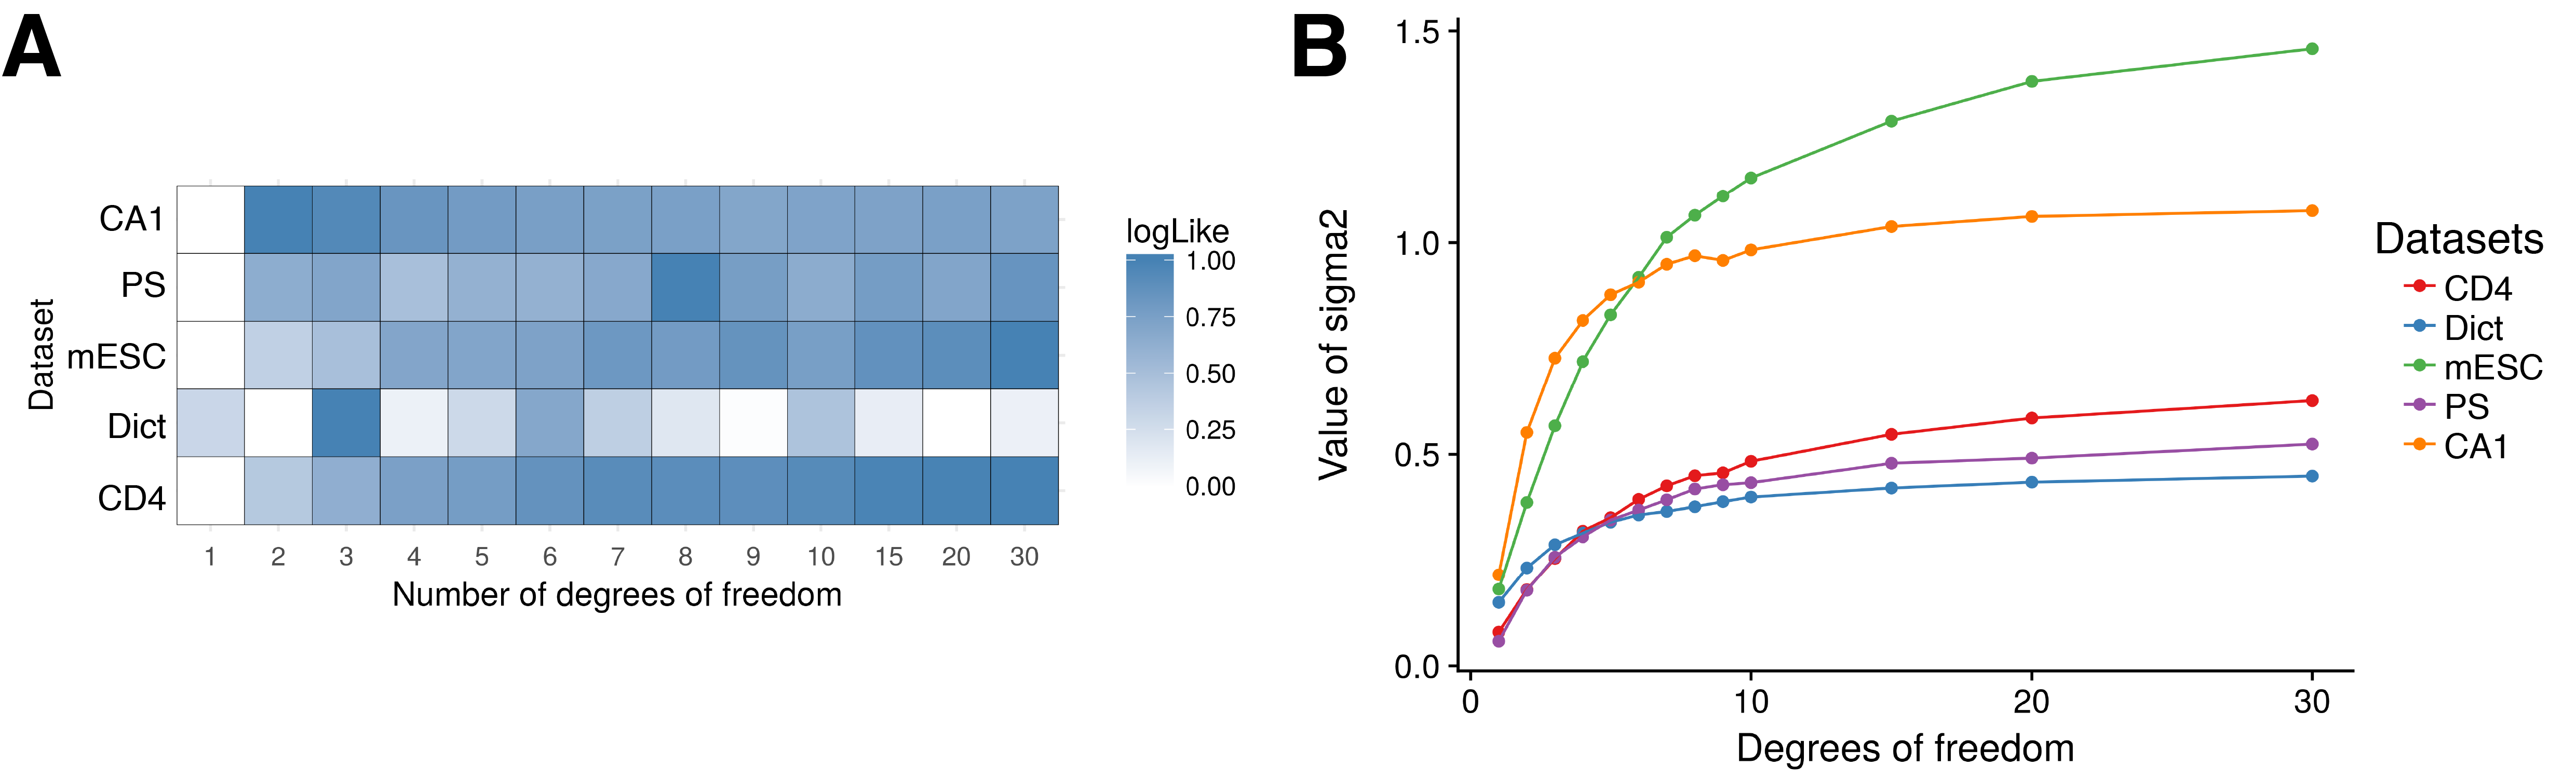
\includegraphics[width=\textwidth]{Fig_5.png}
\caption[Enrichment of under-represented somatic cell types in juvenile samples]{\textbf{Enrichment of under-represented somatic cell types in juvenile samples.} \\
\textbf{(A)} tSNE representation of cells isolated from P10 animals that were mapped to cells from adult mice. Cell types were identified by unbiased, graph-based clustering and annotated after marker gene extraction. SG: Spermatogonia, SC: Spermatocytes, IL: Immature Leydig, PTM: Peritubular Myoid Cells, EC: Endothelial Cells, tMg: testicular Macrophages, \textbf{(B)} Heatmap representation of cell type-specific marker genes. Bolded genes indicate previously described markers for the following cell types: Sertoli cells (\textit{Cst12}), early spermatocytes (\textit{Sycp1}), spermatogonia (\textit{Dmrt1}), immature leydig cells (\textit{Dlk1}), endothelial cells (\textit{Acta2}), peritubular myoid cells (\textit{Tm4sf1}), Leydig cells (Insl3), testicular macrophages (\textit{Cd14}). \textbf{(C)} PCA of spermatogonia (SG) and early spermatocytes (SC 1) from P10 and P15 animals. 
}
\label{fig3:somatic_cells}
\end{figure}

Furthermore, we detect a relative enrichment of spermatogonia compared to other germ cell types at P10 and P15 \textbf{(Fig.~\ref{fig3:somatic_cells}C)}. Using this large amount of stem-cell like cells sampled from different time-points during development allows us to dissect its differentiation programme.

\newpage

\subsection{Spermatogonial differentiation}

In the mouse, spermatogenesis is initiated with the division of a spermatogonial stem cell (SSC or A$_{\text{single}}$) to form first a pair, and then a connected chain of undifferentiated spermatogonia (A$_{\text{paired}}$ and A$_{\text{aligned}}$) \citep{Oakberg1971, DeRooij1973}. These cells have competency to undergo spermatogonial differentiation, which involves six transit-amplifying mitotic divisions generating A$_{1-4}$, Intermediate (In), and B spermatogonia, which then give rise to pre-leptotene spermatocytes (Pl) \citep{DeRooij2000} \textbf{(Fig.~\ref{fig3:cell_staging}C)}. Given this, we expect a high level of heterogeneity within the spermatogonia population but identifying spermatogonial sub-populations in adult testes is greatly complicated by their rarity relative to other germ cell types \citep{Lukassen2018}. However, as shown above, during early juvenile development spermatogonia are relatively enriched, which we exploited to further characterize their heterogeneity \textbf{(Fig. \ref{fig3:1st_wave}A)}. \\

By combining cells from P10 and P15, we obtained 1,186 transcriptional profiles that capture sub-populations during spermatogonial differentiation \textbf{(Fig.~\ref{fig3:spermatogonia}B)}. To jointly analyse transcriptomes of P10 and P15 samples, we performed batch correction between these samples as described above and clustered batch corrected data using a graph-based approach. In order to label the cell types corresponding to the different clusters, we performed marker genes detection using the \emph{findMarker} function in \emph{scran}. By visualizing the individual marker genes, we detect two clusters corresponding to undifferentiated spermatogonia (A$_\textnormal{undiff}$) based on their expression of \textit{Nanos3} and \textit{Zbtb16} \textbf{(Fig. \ref{fig3:spermatogonia}B and C)} \citep{Buaas2004, Lolicato2008}). These cells comprise A$_\textnormal{s}$, A$_\textnormal{paired}$, and A$_\textnormal{aligned}$ spermatogonia that decrease in stemness as they divide and gain competency to differentiate \citep{Suzuki2012}. Additionally, these cells express a number of marker genes also detected in undifferentiated human spermatogonial stem cells, such as \textit{Gfra1}, \textit{Bcl6} and \textit{Id4} \citep{Guo2017}. Based on the expression of \textit{Stra8} (Stimulated by retinoic acid 8), we can map the point at which spermatogonial differentiation is induced (A$_\textnormal{aligned}$-to-A$_\textnormal{1}$ transition), thus marking the beginning of differentiating spermatogonia (A$_\textnormal{diff}$) \citep{Endo2015} \textbf{(Fig. \ref{fig3:spermatogonia}B)}. A$_\textnormal{diff}$ are marked by the expression of \textit{Sohlh1} \citep{Ballow2006} and are highly proliferative, generating A$_\textnormal{1-4}$, Intermediate and B spermatogonia. Late differentiating spermatocytes express \textit{Dmrtb1}, which mediates the mitosis-to-meiosis transition and quickly disappears in pre-leptotene spermatocytes \textbf{(Fig. \ref{fig3:spermatogonia}B)}. This latter population shows a second increase in \textit{Stra8} expression levels, which is necessary for initiation of meiosis \textbf{(Fig.~\ref{fig3:spermatogonia}B and C)} \citep{Anderson2008, Endo2015, Zhang2014}. 

\newpage

\begin{figure}[!h]
\centering
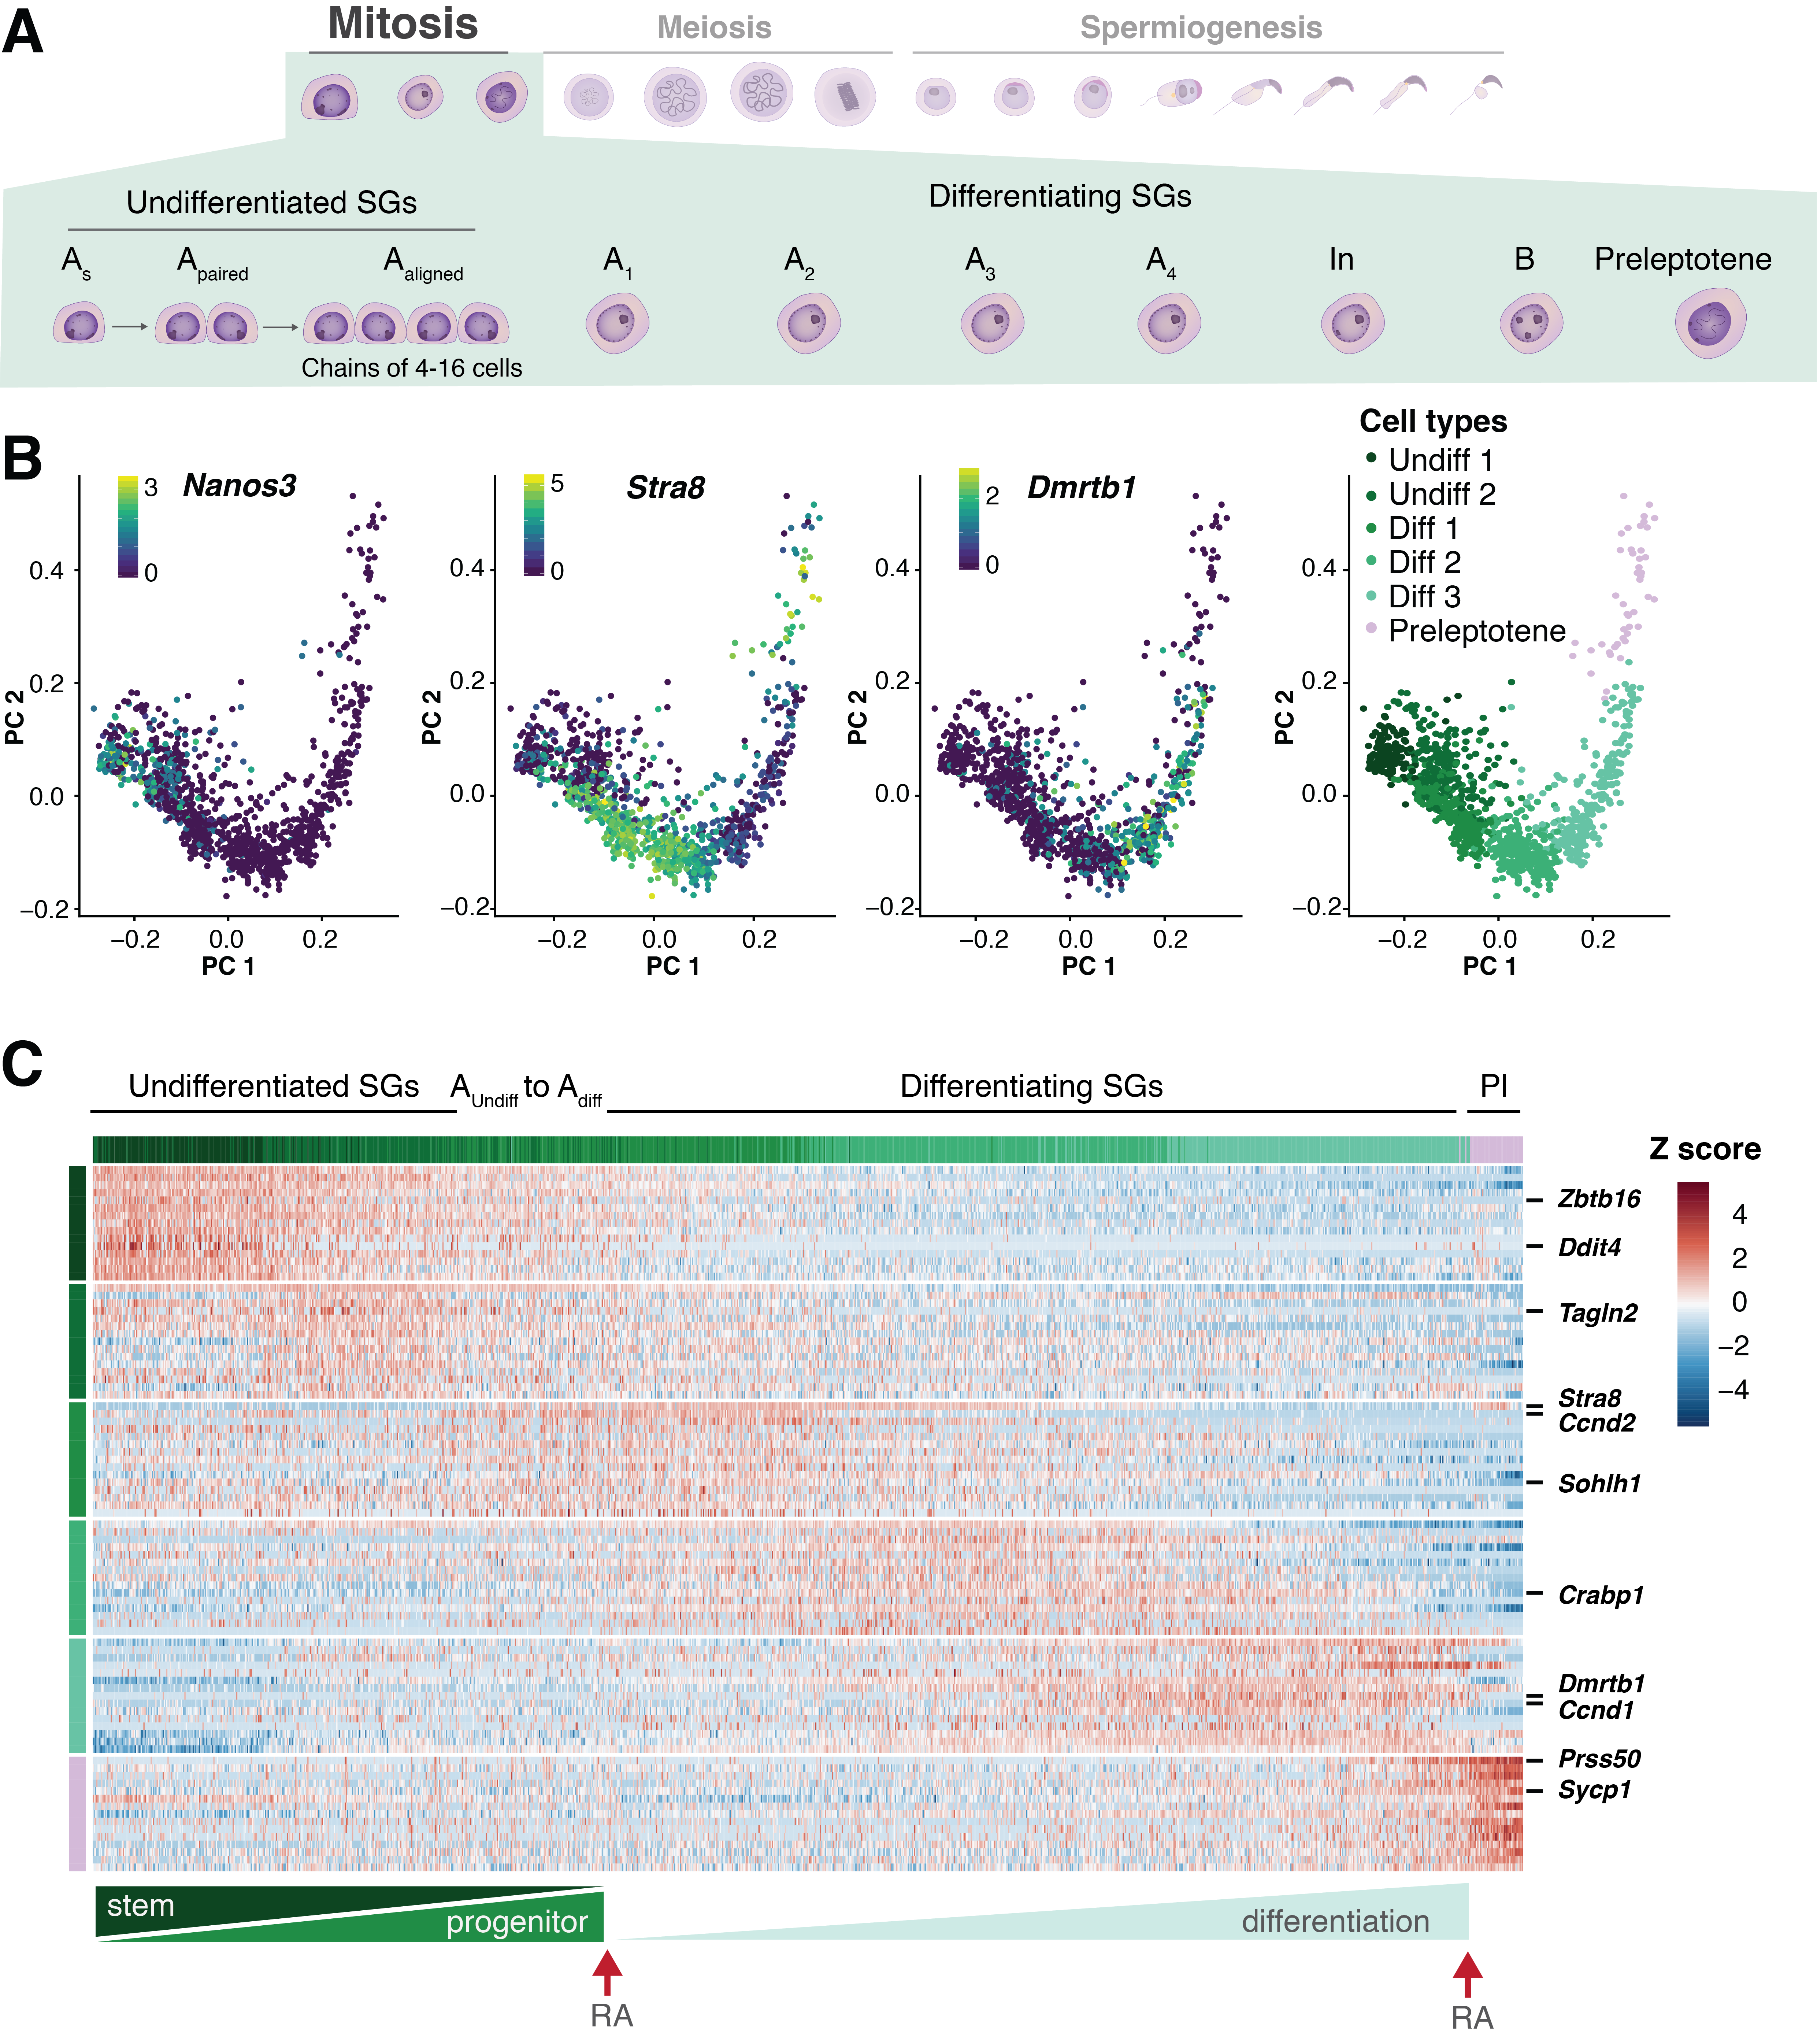
\includegraphics[width=0.9\textwidth]{Fig_6.png}
\caption[Cellular heterogeneity during spermatogonial differentiation]{\textbf{Cellular heterogeneity during spermatogonial differentiation.}\\
\textbf{(A)} Schematic representation of spermatogonial differentiation including sub-stages of undifferentiated (A$_\textnormal{s}$, A$_\textnormal{paired}$, A$_\textnormal{aligned}$) and differentiating (A$_\textnormal{1}$, A$_\textnormal{2}$, A$_\textnormal{3}$, A$_\textnormal{4}$, In, B) spermatogonia (SGs) as well as pre-leptotene spermatocytes (Pl), \textbf{(B)} Sub-structure detection in spermatogonia isolated from P10 and P15 animals. PCA was computed on transcriptomes after batch correction between P10 and P15 samples. The first three panels represent expression of known marker genes for undifferentiated (Undiff, \textit{Nanos3}) and differentiating (Diff, \textit{Stra8} and \textit{Dmrtb1}) spermatogonia. The colour scale shows log$_2$-transformed, normalized counts. The last panel overlays cluster identity by sub-clustering batch-corrected transcriptomes of spermatogonia, \textbf{(C)} Z factor of normalized expression counts of the top 15 marker genes per cell cluster. Column and row labels represent the cell clusters identified in the last panel of (B). The lower bar indicates the gradual differentiation from undifferentiated spermatogonia to pre-leptotene cells driven by two retinoic acid (RA) signals. }
\label{fig3:spermatogonia}
\end{figure}

\newpage

\subsection{Leptotene and zygotene spermatocytes}

The transition between differentiating spermatogonia and spermatocytes is a gradual process that occurs in stage VIII tubules when B spermatogonia divide and form pre-leptotene spermatocytes \citep{Anderson2008, Baltus2006}. When visualizing the first two components of a PCA, we did not observe a continuous differentiation trajectory bridging spermatogonia to spermatocytes \textbf{(Fig.~\ref{fig3:somatic_cells}C)} which indicates a possible loss of cells that characterise the transition between these two cell-types. One possible explanation is that leptotene and zygotene spermatocytes have decreased transcriptional activity \citep{Kierszenbaum1974, Monesi1965}, and are thus likely to be classified as empty droplets by the 10X CellRanger pipeline. \\

To capture these transcriptionally quiescent cells and as explained above, we used the \emph{emptyDrops} function from the \emph{DropletUtils} R package to distinguish between droplets capturing genuine cells with low transcriptional complexity \emph{versus} empty droplets containing only ambient mRNA \citep{Lun2018}. Applying this approach increased the number of early spermatocytes in all samples and, in particular, identified a population of cells connecting spermatogonia and spermatocytes at the predicted position in the cell trajectory \textbf{(Fig.~\ref{fig3:emptyDrops}A-C)}. Especially in the P15 sample, we strongly enrich for leptotene and zygotene spermatocytes when including smaller cells into the analysis. Due to low transcriptional complexity, these two cell-types cluster together which makes it hard to detect a clear mitosis-to-meiosis transition \textbf{(Fig.~\ref{fig3:emptyDrops}B and C)}. As expected for leptotene and zygotene spermatocytes, these cells show high mRNA levels for genes involved in synaptonemal complex formation, chromosome synapsis and DNA double-strand break (DSB) formation such as \textit{Sycp1}, \textit{H2afx} and \textit{Hormad1} \citep{Daniel2011, Mahadevaiah2001, Vries2005} \textbf{(Fig.~\ref{fig3:emptyDrops}D)}.\\

In addition to early spermatocytes, droplets with lower transcriptional complexity also captured late condensing spermatids. As mentioned above, these late stages of spermiogenesis are characterized by continuous degradation of RNA after transcriptional shut-down at the round-to-elongating transition \citep{Steger1999} \textbf{(Fig.~\ref{fig3:emptyDrops}E)}. Nevertheless, including droplets with low transcriptional complexity increases the risk of including low-quality cells and debris. In our case, the large cluster of unidentified cells in \textbf{Fig.~\ref{fig3:emptyDrops}A} could represent membrane vesicles containing RNA at the end of spermiogenesis that form during a process termed "cytoplasmic extrusion" \citep{Rengan2012}.\\

\newpage

\begin{figure}[!h]
\centering
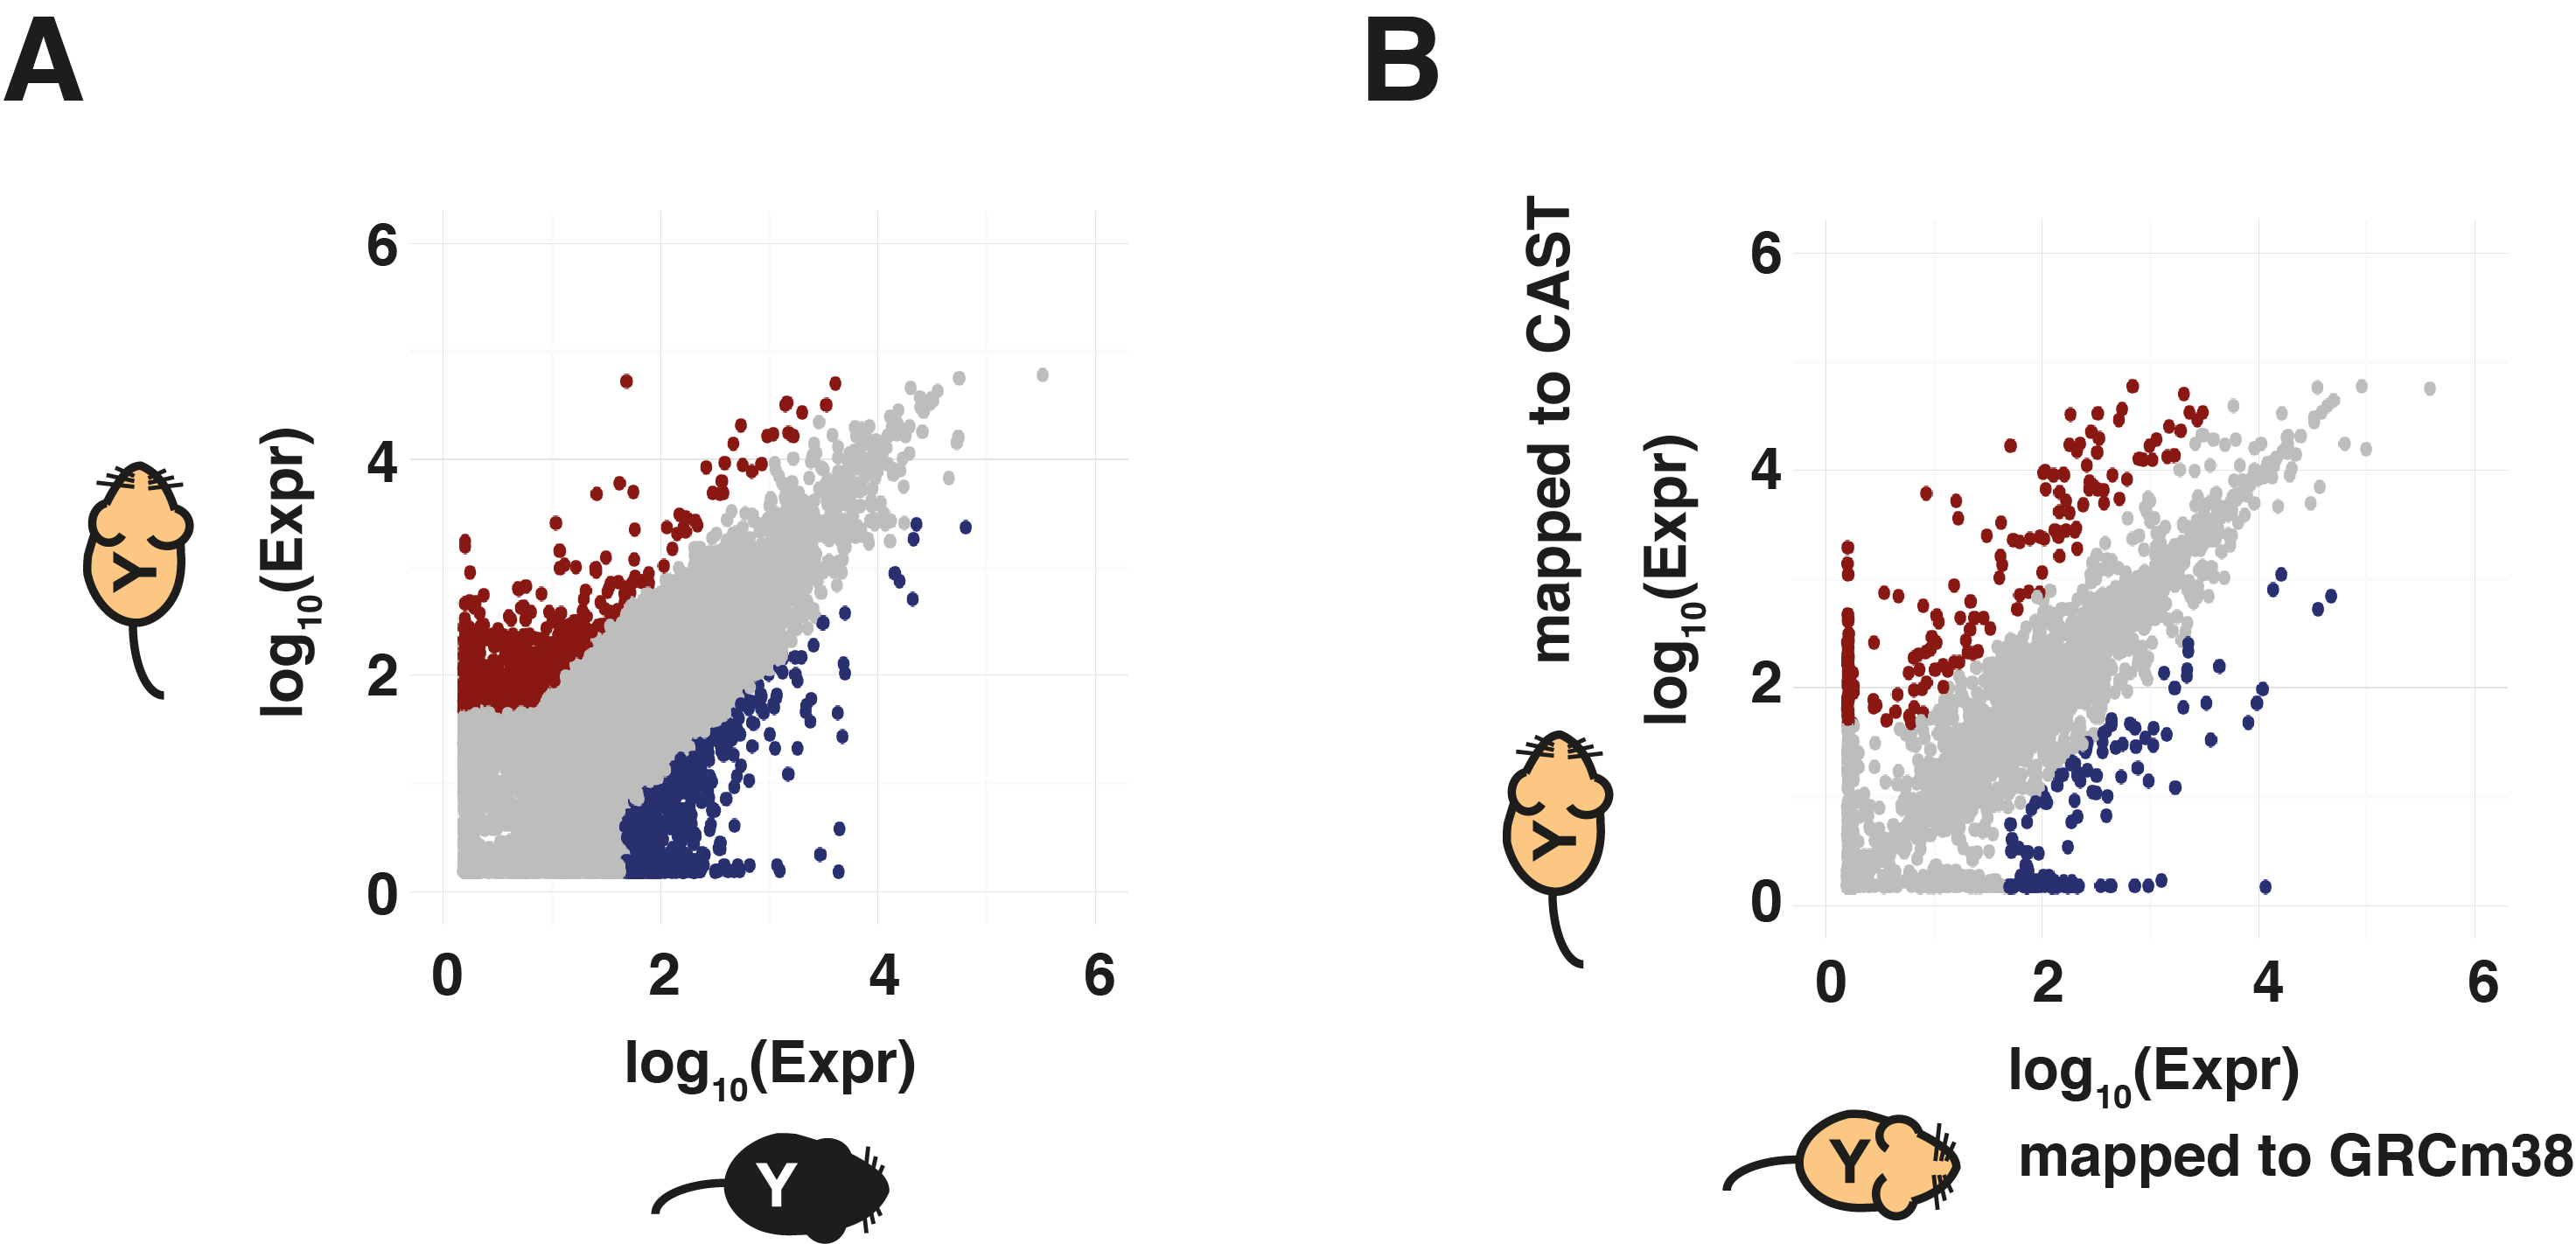
\includegraphics[width=0.8\textwidth]{Fig_7.png}
\caption[Transcriptionally silent cell types in spermatogenesis.]{\textbf{Detection of transcriptionally silent cell types in scRNA-Seq data.} \\
\textbf{(A)} tSNE representation of cells selected by the \emph{emptyDrops} filtering strategy. Coloured dots represent annotated cell types detected using the default \emph{CellRanger} filtering pipeline while black dots represent cells detected by the \emph{emptyDrops} filtering. SG: Spermatogonia, SC: Spermatocytes, IL: Immature Leydig, PTM: Peritubular Myoid Cells, EC: Endothelial Cells, tMg: testicular Macrophages, \textbf{(B)} tSNE representation of emptyDrops filtered cells from the P15 sample. Cell colouring corresponds to clustering performed on this sample. Undiff SG: undifferentiated spermatogonia, Diff SG: differentiating spermatogonia, \textbf{(C)} PCA representation of spermatogonia and spermatocytes detected in the P15 sample after \emph{emptyDrops} filtering. Labelling corresponds to the clusters shown in (B), \textbf{(D)} Leptotene and zygotene spermatocyte marker gene expression. The colour scale represents log$_2$-transformed, normalized counts, \textbf{(E)} Visualization of the number of genes expressed (> 0 counts) per cell.}
\label{fig3:emptyDrops}
\end{figure}

\newpage

\section{Characterization of male meiosis}

After characterising the major germ and somatic cell types, we next profiled the transcriptional programmes of known developmental processes during spermatogenesis. These include firstly meiosis and later on spermiogenesis which will be analysed and discussed in the next section.\\

The mitotic expansion of spermatogonia produces large numbers of spermatocytes, which then undergo male meiosis where two consecutive cell divisions give rise to four haploid spermatids. In contrast to mitotic cell divisions, prophase of meiosis I is extremely prolonged, lasting up to 10 days in male mice \citep{Soh2017}. Furthermore, meiosis includes programmed DNA double strand break (DSB) formation, homologous recombination, and chromosome synapsis \citep{Marston2004}, which represent molecular processes to induce genetic variation between offsprings. Most meiotic processes have been histologically described, but a full transcriptional characterization of spermatocytes undergoing meiosis is lacking. \\

The continuum of sampled cell types allows us to perform in-depth characterisation of transcriptional changes that occur during meiosis. For this, we ordered spermatocytes along their differentiation trajectory by fitting a principal curve \citep{Hastie1989} to the first 3 principal components using the \emph{principal.curve} function implemented in the \emph{princurve} R package. This approach allows us to order cells along the developmental trajectory. The directionality of the trajectory was inferred using prior information based on the cluster annotation. Here, the ordering of cell types is as follows: leptotene spermatocytes (SCs, not present in CellRanger filtered data), zygotene SCs, pachytene SCs, diplotene SCs and finally cells in metaphase \textbf{(Fig.~\ref{fig3:meiosis}A)}. \\

To detect molecular processes that occur during meiosis, we first profiled the overall transcriptional rate before dissecting changes in expression on a gene-specific level. As shown before \citep{Xia2018}, we identified a strong increase in the number of genes expressed as spermatocytes progress through prophase, with the highest number being expressed immediately before the cells divide \textbf{(Fig.~\ref{fig3:meiosis}A)}. Using this as a proxy for active transcription, we identified diplotene spermatocytes, which are the latest cell type in prophase I in which RNA synthesis is occurring \citep{Monesi1965}. 

\newpage

We used the increase and later decrease in transcription as a guide for the progressive changes in transcription throughout meiosis. Therefore, to detect functional genes that influence this process, we correlated each gene’s normalised expression level to the number of genes expressed. For this, we used the \emph{correlatedPairs} function implemented in \emph{scran} \citep{Lun2016}. First, we constructed an empirical null distribution using the \emph{correlateNull} function implemented in \emph{scran}. Next, we tested the observed Spearman’s $\rho$ for each gene against this null distribution. Genes with $\rho$ < -0.3 and a Benjamini-Hochberg corrected empirical p-value < 0.1 were considered as negatively correlated and genes with $\rho$ > 0.3 and a Benjamini-Hochberg corrected empirical p-value < 0.1 were considered as positively correlated.\\

As expected, previously known marker genes for early meiotic processes such as \textit{Hormad1} and \textit{Sycp3} decreased in expression during Prophase I, whereas \textit{Pou5f2} and \textit{Tcte2}, a male-meiosis specific gene \citep{Braidotti1997} increased in expression \textbf{(Fig.~\ref{fig3:meiosis}B)}. Supporting our identification of diplotene spermatocytes, \textit{Pou5f2} has previously been shown to be specifically expressed during a 36- to 48-hour period preceding the meiotic cell division \citep{Andersen1993}. \\

In the next step, we performed less biased analysis and detected marker genes for each of the spermatocyte sub-cell-types. Despite the overall increase in transcription, we observed distinct temporal expression patterns when visualizing these specific marker genes for individual spermatocyte populations. Even within pachytene spermatocytes at different stages in their developmental progression, there exists substantial heterogeneity \textbf{(Fig.~\ref{fig3:meiosis}C)}. As expected, early spermatocyte markers (SC 1 and SC 2) were enriched for genes with known functions in male or female fertility such as \textit{Piwil1} (\textit{Miwi}), \textit{Cks2}, \textit{Sycp1}, reflecting a history of intensive investigation \citep{Deng2002, Spruck2003, Vries2005}. We performed literature search and used the database \url{www.mousephenotype.org} to annotated genes regarding their sterility phenotype. \\

In sum, we dissected the transcriptional heterogeneity within spermatocytes undergoing meiosis and found numerous genes to be associated with this developmental process.

\newpage

\begin{figure}[!h]
\centering
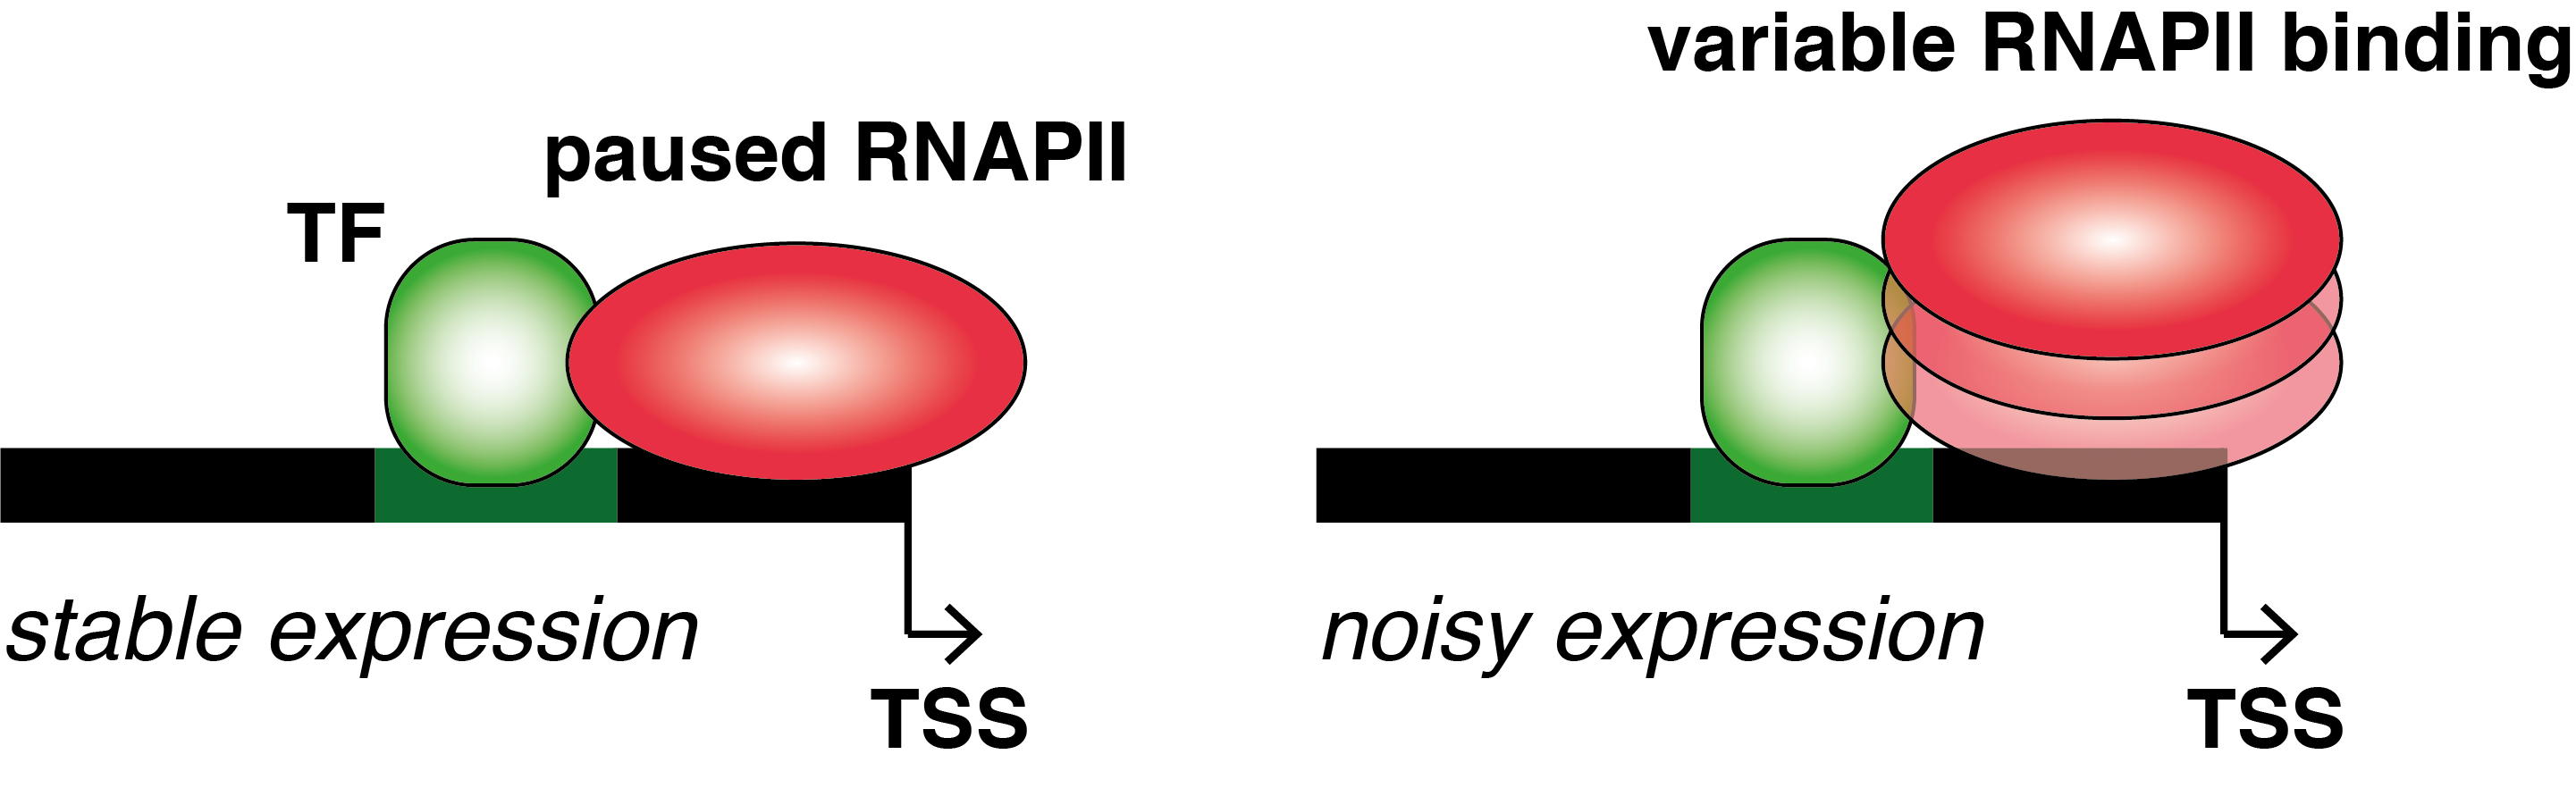
\includegraphics[width=0.9\textwidth]{Fig_8.png}
\caption[Gene expression dynamics during male meiosis]{\textbf{Gene expression dynamics during male meiosis.} \\
\textbf{(A)} Number of genes expressed per spermatocyte. Cells are ordered by their developmental progression during meiotic prophase until metaphase, \textbf{(B)} Expression of genes that are negatively or positively correlated with the number of genes expressed during meiotic prophase (negatively correlated: $\rho$ < -0.3, Benjamini-Hochberg corrected empirical p-value < 0.1; positively correlated: $\rho$ > 0.3, Benjamini-Hochberg corrected empirical p-value < 0.1). Per category, two genes are visualized. The colour gradient represents log$_2$-transformed, normalized counts, \textbf{(C)} Heatmap visualizing the Z factor scaled expression of the top 15 marker genes per cell type. Row and column labels correspond to the different populations of spermatocytes (SC). M: Metaphase. Genes are labelled based on their fertility phenotype: pink – infertile or sub-fertile in females, light blue - infertile or sub-fertile in males, dark green - infertile or sub-fertile in both males and females. The sterility phenotype was annotated using \url{www.mousephenotype.org.}}
\label{fig3:meiosis}
\end{figure}

\section{Transcriptional dynamics during spermiogenesis}
\label{sec3:spermiogenesis}

Once the meiotic divisions resulted in the production of four haploid cells, round spermatids progress to form first elongating and finally mature sperm during a process termed "spermiogenesis" \textbf{(Fig.~\ref{fig3:spermiogenesis}A)}. A key event during spermiogenesis is chromatin condensation, which is required to package the haploid genome into the confined space of the sperm nucleus. Our data allowed us to dissect at high-resolution the transcriptional regulation needed for gradual chromatin remodelling during spermatid differentiation, involving the replacement of canonical histones by histone variants followed by transition proteins and eventually protamines \citep{Balhorn2007, Kennani2017}. This chromatin remodelling later on induces a transcriptional shut-down where changes in RNA content are purely driven by degradation \citep{Steger1999}.

\subsection{Expression of chromatin components during spermiogenesis}

For this, we first explored how expression of histone variants changed throughout early spermatid maturation \textbf{(Fig.~\ref{fig3:spermiogenesis}A)}. Similar to the developmental ordering presented in the previous section, we ordered cells by fitting a principle curve to the first three principal components calculated on S1-S14 spermatids. Annotations for histone variants and canonical histones were taken from El Kennani \emph{et al.}, 2017 \citep{Kennani2017}. Multiple variants of H3 and H2A are expressed in spermatocytes \citep{Greaves2006, Mahadevaiah2001, Tang2015}, and our data showed that many of these histones are highly expressed in early round spermatids. For instance, Histone H3.3 is a histone variant consisting of two genomic copies (\textit{H3f3a} and \textit{H3f3b}). Across spermatogenesis, we observed distinct expression patterns for the two genes, with \textit{H3f3a} being consistently high until the transcriptional shut-down at spermatid stage S10. In contrast, \textit{H3f3b} showed a much more dynamic expression profile, starting high in spermatocytes, dropping throughout meiotic prophase, followed by up-regulation in round spermatids \textbf{(Fig.~\ref{fig3:spermiogenesis}B)}. Although both genes have been implicated in male fertility, the phenotypes associated with perturbations of the more dynamically regulated paralog \textit{H3f3b} are much more severe \citep{Tang2015, Yuen2014}.\\

When profiling the expression of canonical histones, we detected increased expression for \textit{Hist1h2bp} and \textit{Hist1h4a} that showed a distinct up-regulation during early and mid-spermiogenesis \textbf{(Fig.~\ref{fig3:spermiogenesis}C)}. Canonical histones are typically transcribed in a replication-dependent manner during S phase \citep{Marzluff2002}, thus the atypical expression during spermiogenesis could suggest important roles as replacement histones during chromatin remodelling. Nevertheless, canonical histones appeared to be the set of annotated histones that is least correlated to the developmental trajectory \textbf{(Fig.~\ref{fig3:spermiogenesis}A)}.

\newpage

\begin{figure}[!h]
\centering
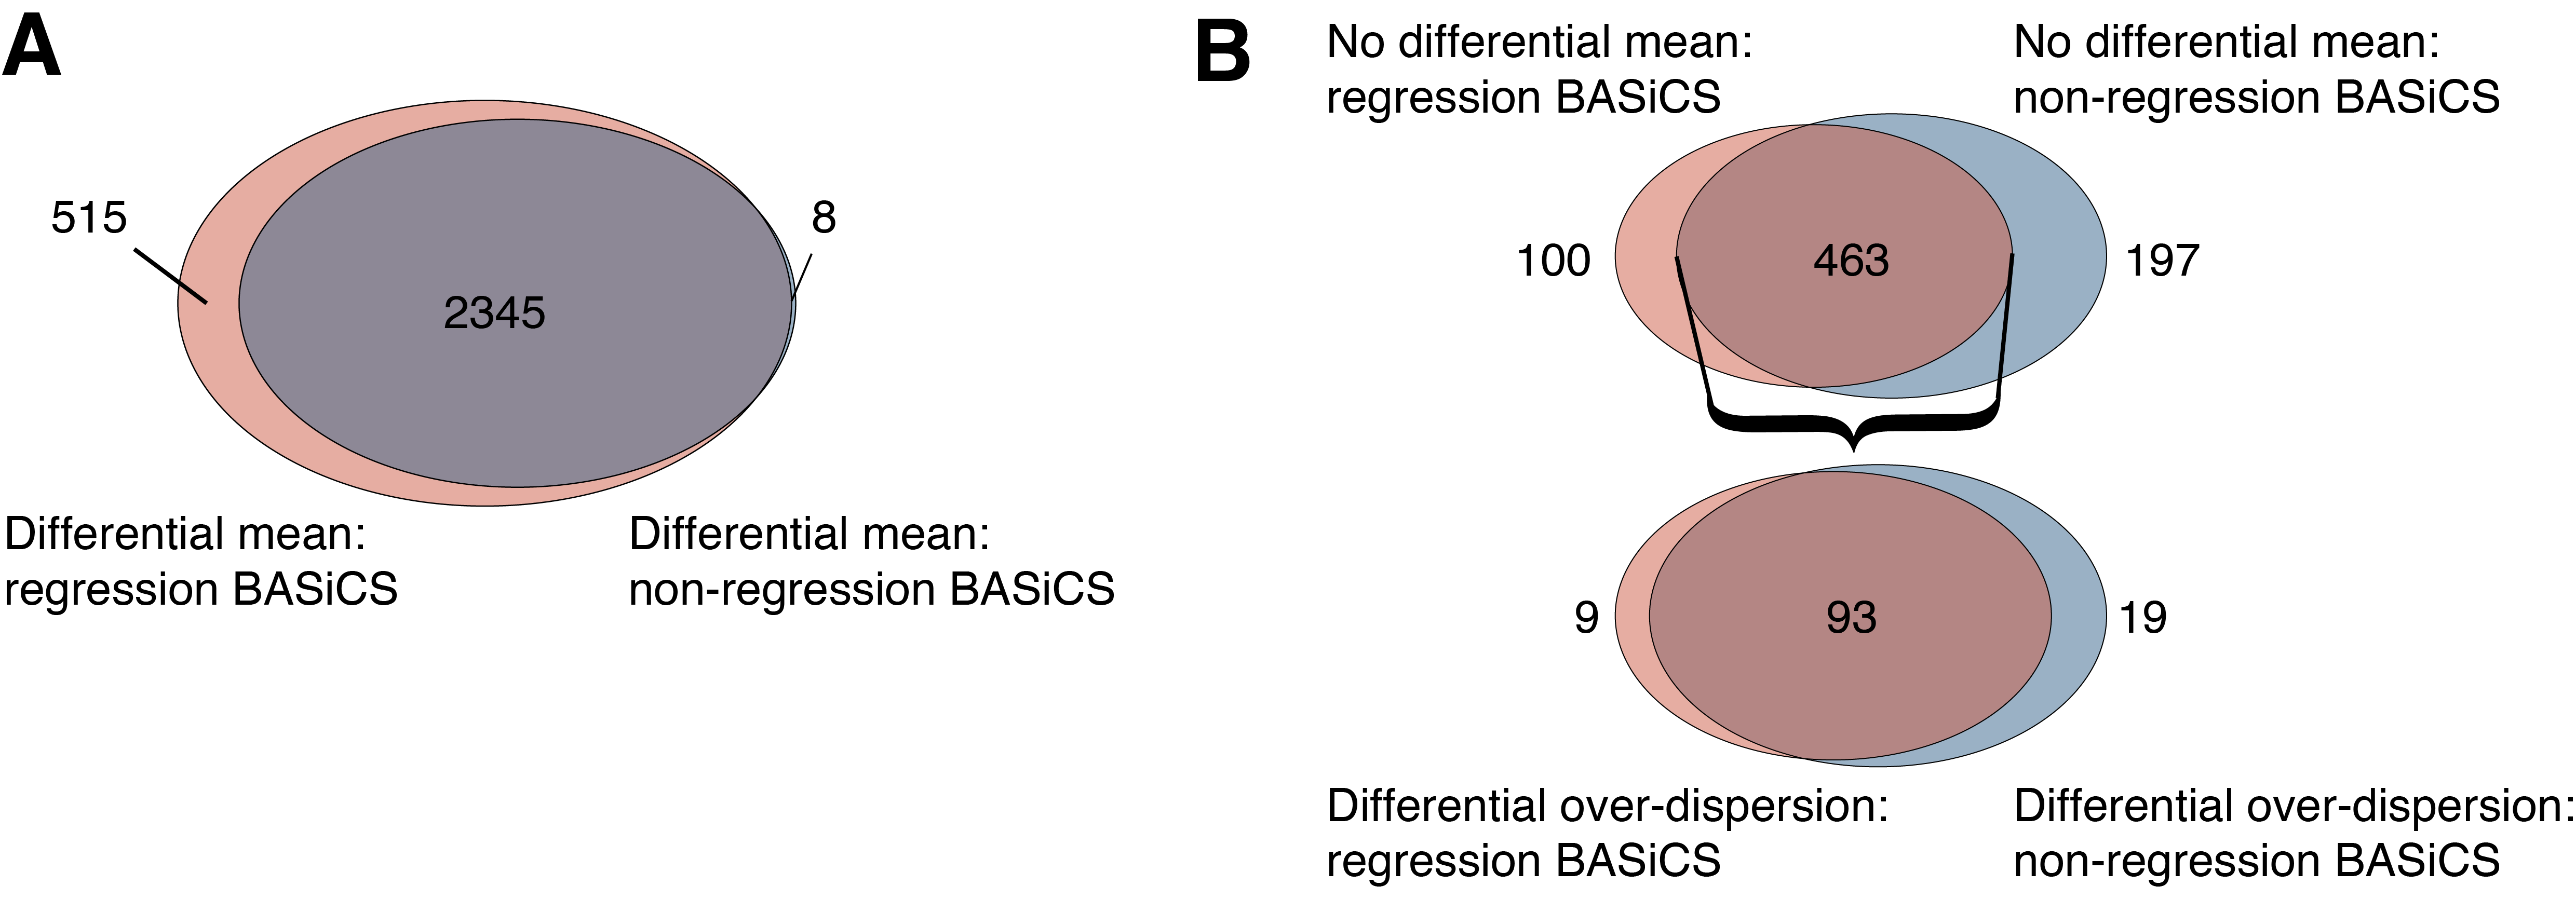
\includegraphics[width=0.85\textwidth]{Fig_9.png}
\caption[Transcriptional dynamics and chromatin remodelling during spermiogenesis]{\textbf{Transcriptional dynamics coupled to chromatin remodelling during spermiogenesis.} \\
\textbf{(A)} Z factor scaled, normalized expression of histone variants (H1, H2A, H2B, H3), canonical histones, transition proteins (Tnp) and protamines (Prm) during spermiogenesis. Cells were ordered based on their developmental trajectory ranging from round spermatids (S1-S8) to elongating spermatids (S9-S14), \textbf{(B)} Expression of \textit{H3f3a} (middle panel) and \textit{H3f3b} (right panel) across the different germ cell populations, \textbf{(C)} Similar visualization as in (B) for \textit{Hist1h4a} expression across germ cells. }
\label{fig3:spermiogenesis}
\end{figure}

\newpage

We next profiled the transcriptional dynamics of testis-specific histone variants. They showed highest expression in elongating spermatids, with most variants increasing strongly in expression from S5 onwards. While some variants had a consistently high expression level, \textit{Hils1} and \textit{H1fnt} decreased in expression towards the late stages, similarly to \textit{Tnp1} and \textit{Tnp2} \citep{Zhao2004}. Both histone variants are important for male fertility, and \textit{Hils1} has previously been shown to interact with \textit{Tnp1} \citep{Tanaka2005}. In contrast, three testis-specific histone variants \textit{Hypm}, \textit{H2afb1} and \textit{H2bl1} (\textit{1700024p04rik}) showed consistently high expression until the end of differentiation similar to protamines, suggesting these variants contribute to the final genome condensation.

\subsection{Identifying the point of transcriptional shut-down}

As a consequence of chromatin condensation, transcription ceases in spermatids at the round to elongating switch, consistent with the lack of active RNA Pol II at S10 and later stages \citep{DottermuschHeidel2014}.
By fitting a smooth regression (loess) to the number of genes expressed per cells along the differentiation trajectory, we easily identified the point of transcriptional shut-down. The number of expressed genes is stable until approximately S9 before gradually declining by roughly 50\% \textbf{(Fig.~\ref{fig3:transcriptional_shutdown}A)}. In the 8 days following transcriptional shut-down, spermatids still need to undergo drastic morphological changes, including the assembly of sperm-specific structures such as the flagellum, before mature testicular sperm can be released into the lumen \citep{ODonnell2014}. To achieve this in the absence of active transcription, spermatids store large amounts of mRNAs in a perinuclear RNA granule termed the chromatoid body or \emph{nuage} \citep{Kotaja2007}. RNA stored in the chromatoid body is then released for translation, suggesting that these molecules may play vital roles during late stages of spermiogenesis. However, identifying the RNAs that are stored has been hindered by difficulties in purifying late spermatids. \\

By correlating normalized gene expression against the number of genes expressed, we identified a large number of genes that gradually decrease in relative expression after transcriptional shut-down. We reasoned that transcripts where the relative expression after transcriptional shut-down appeared to increase are likely protected from degradation \textbf{(Fig. \ref{fig3:transcriptional_shutdown}B)}. This included genes with well-known spermiogenesis-specific functions. Among those that relatively increase in expression, we find transition proteins and protamines that are involved in chromatin condensation. Furthermore, we detect genes that are involved in the development of sperm motility such as \textit{Akap4} and \textit{Cabs1} \citep{Kawashima2009, Miki2002}. 

\newpage

\begin{figure}[!h]
\centering
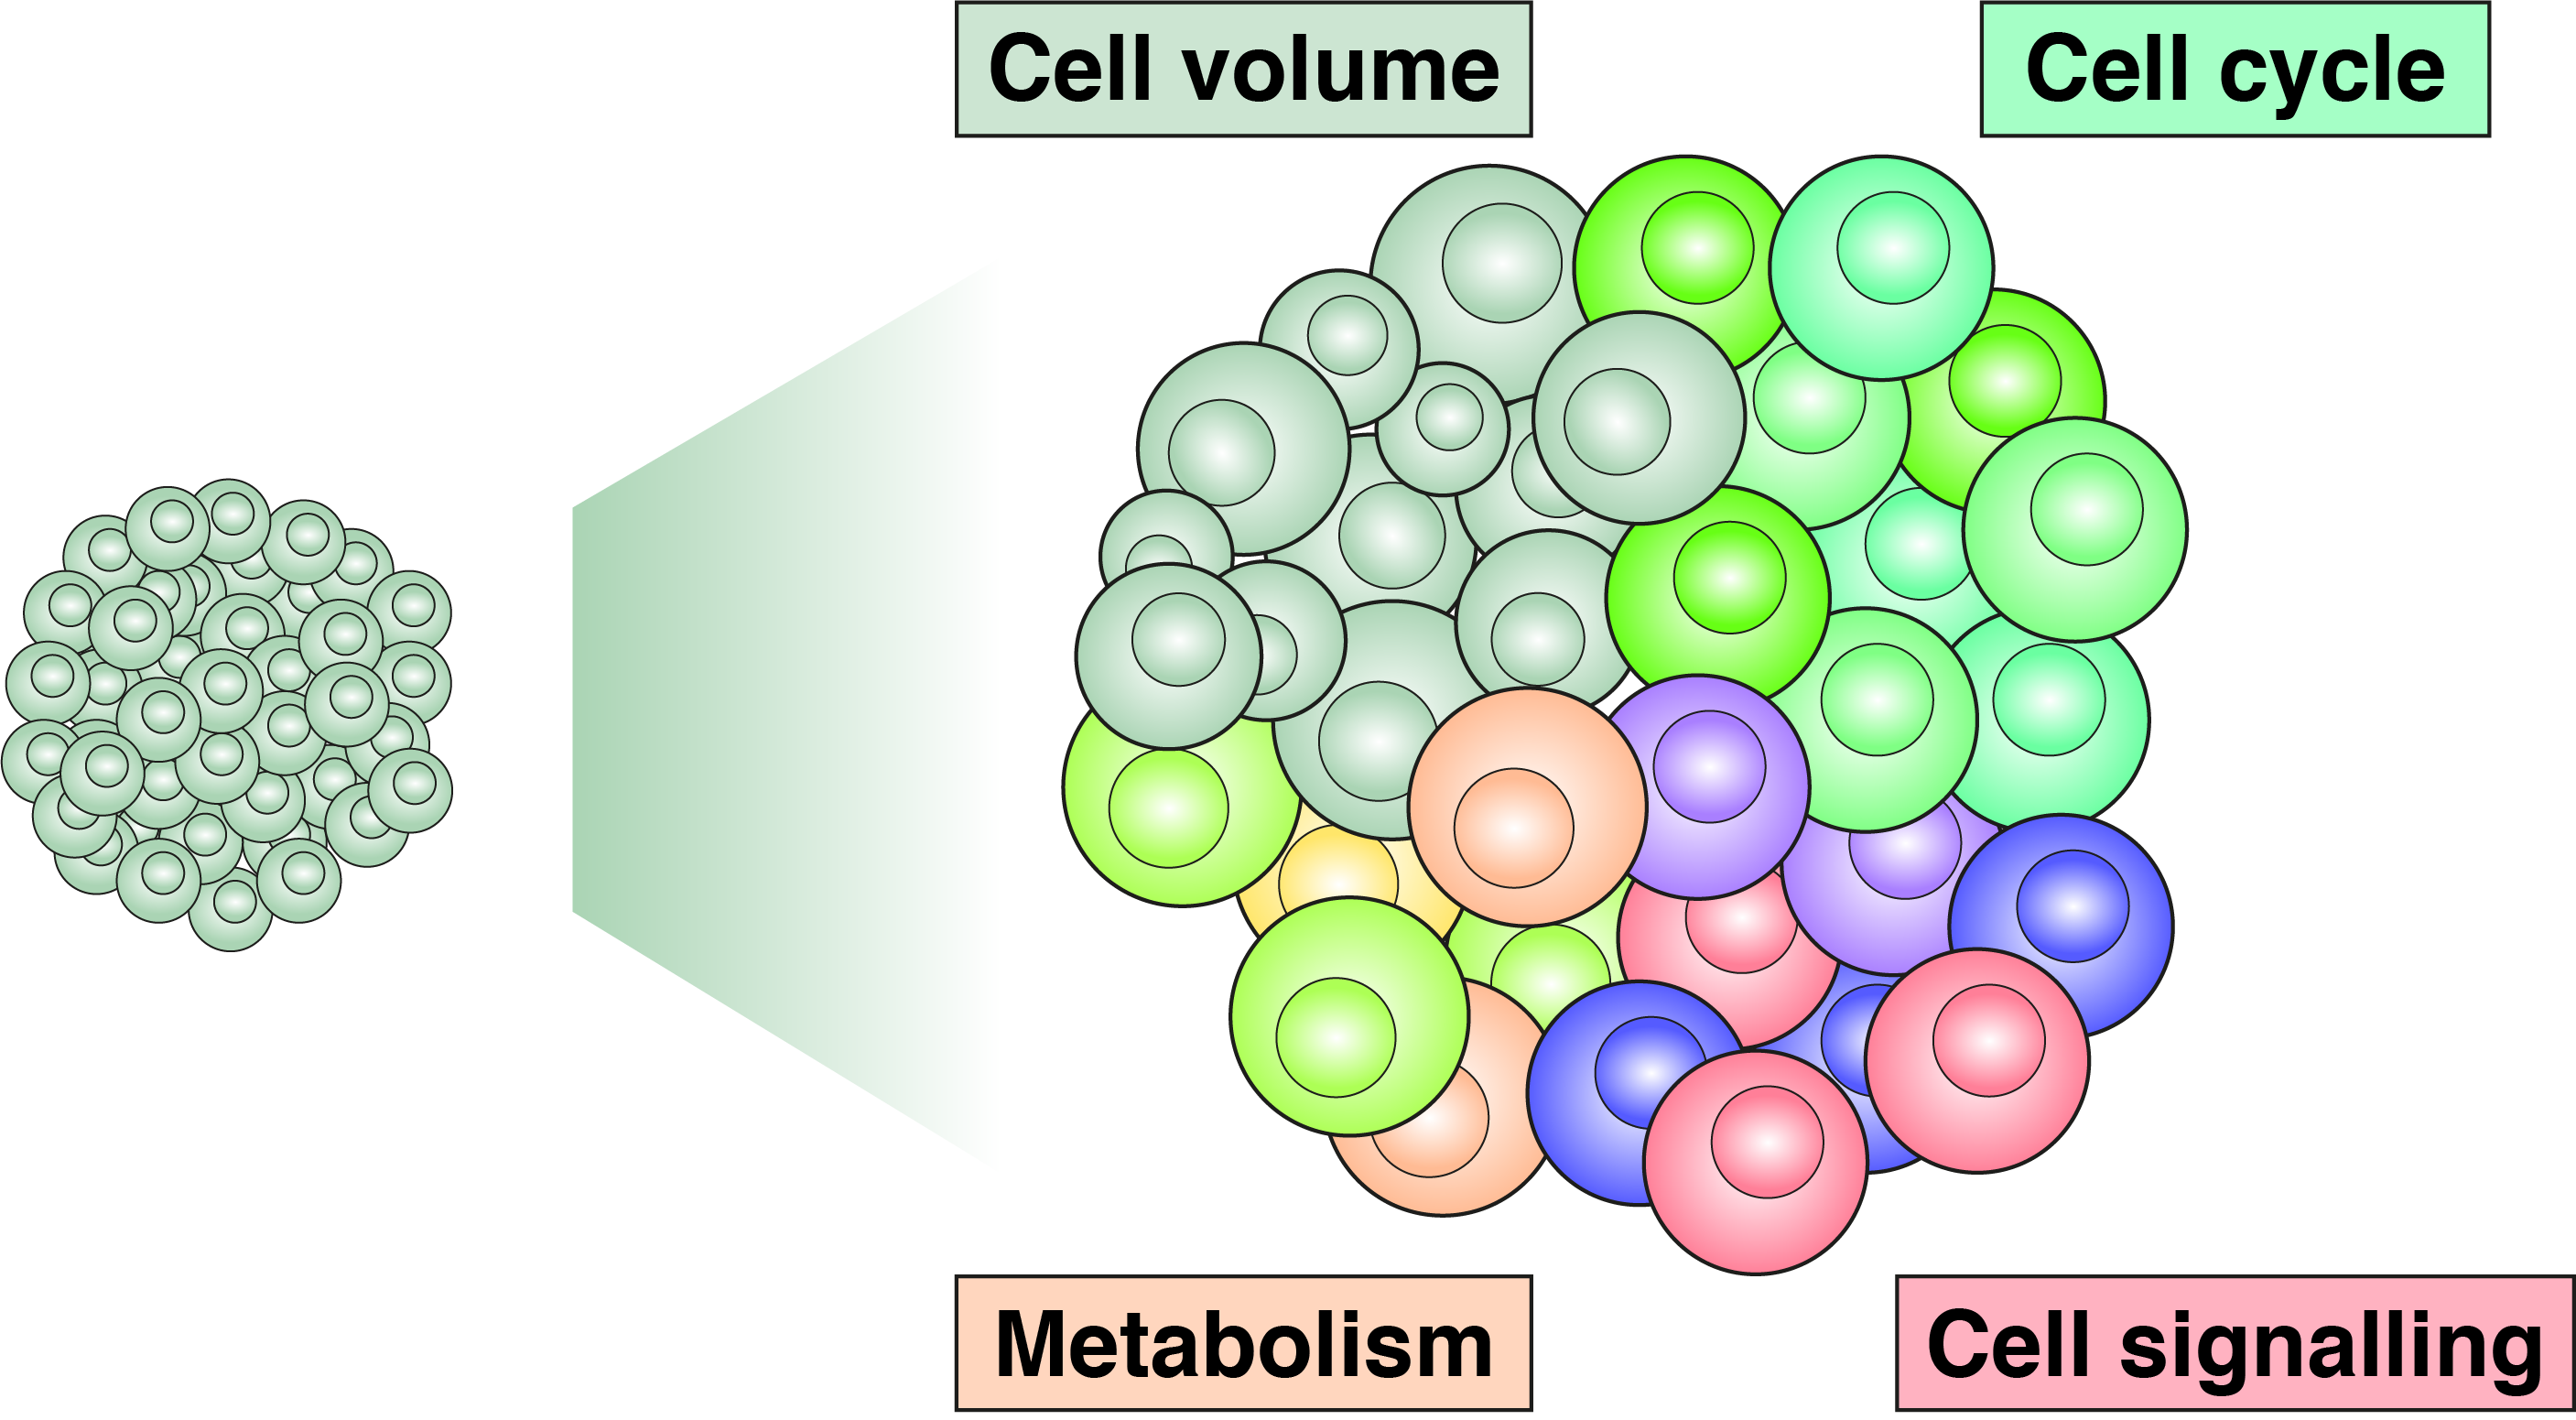
\includegraphics[width=\textwidth]{Fig_10.png}
\caption[Transcriptional shut-down during spermiogenesis]{\textbf{Transcriptional shut-down during spermiogenesis.} \\
\textbf{(A)} Number of genes expressed per spermatid. Cells were ordered based on their developmental trajectory. Red line indicates a smooth regression (loess) fit, \textbf{(B)} For each gene, its normalised expression per cell was correlated with the number of genes expressed per cell. Genes were ordered based on the correlation coefficient and grouped into 9 sets. Z factor scaled expression was averaged across genes within each gene set. Vertical dashed line indicates transcriptional shut-down between S9 and S10.}
\label{fig3:transcriptional_shutdown}
\end{figure}

With this analysis, we explored transcriptional processes occurring throughout the process of spermiogenesis that (i) regulate the expression of chromatin components and (ii) lead to the degradation of unneeded transcripts.

\newpage

\section{Meiotic silencing dynamics of sex chromosomes}

A male-specific feature of meiosis is the transcriptional silencing of sex chromosomes, followed by partial reactivation in post-meiotic spermatids. This process is termed meiotic sex chromosome inactivation (MSCI), and is caused by asynapsis of the sex chromosomes, leading to accumulation of phosphorylated H2AFX and the formation of the sex body \citep{Hamer2003} \textbf{(Fig.~\ref{fig3:X_reactivation}A)}. We next profiled transcriptional changes mediated by the inactivation and reactivation of the sex chromosomes in single-cell and bulk RNA-Seq data. \\

To assess overall transcriptional dynamics of the sex chromosomes, we computed the ratio of expression from the X, Y chromosome and chromosome 9 to all autosomes. For this, we selected genes that were expressed in more than 30\% of spermatogonia or 30\% of spermatids, the cell types with detectable sex chromosome expression. For each cell, the mean expression across these genes per chromosome was calculated. Mean expression of the sex chromosomes and chromosome 9 was divided by mean expression across all autosomes. By plotting the ratio of gene expression from the X or Y chromosomes compared to all autosomes, the inactivation and re-activation status of the sex chromosomes can be inferred \textbf{(Fig.~\ref{fig3:X_reactivation}B)}. \\

The X chromosome is partially up-regulated in spermatogonia as described by Sangrithi \emph{et al.}, 2017 (X:A ratio < 1) \citep{Sangrithi2017}, followed by transcriptional silencing in spermatocytes. Throughout spermiogenesis, expression from the X gradually increases, reaching X:A ratios comparable to spermatogonia, therefore suggesting a substantial reactivation of the X chromosome in post-meiotic spermatids. We detect similar behaviour for the Y chromosome but due to the small number of expressed genes, the signal is noisier \textbf{(Fig.~\ref{fig3:X_reactivation}B)}. In comparison, chromosome 9 shows consistent expression across all cell types throughout spermatogenesis (9:A $\approx$ 1).\\

Transcriptional silencing was originally thought to persist throughout post-meiotic development \citep{Greaves2006, Turner2006}. However, several genes have been shown to be re- or \emph{de novo} activated in spermatids, some of which are dependent on \textit{Rnf8} (Ring finger protein 8) and/or \textit{Scml2} (Sex comb on midleg-like 2) \citep{Hasegawa2015, Sin2012, Sin2015}. The precise timing and order of the transcriptional reactivation of \emph{de novo} escape genes during spermiogenesis has not been explored. We therefore first classified \emph{de novo} activated escape genes using bulk RNA-Seq data and profiled their temporal expression directly following meiosis.\\

Profiling whole-testis transcriptomes of juvenile mice sampled every two days during the first wave of spermatogenesis allowed the sensitive detection of spermatid-specific escape genes \textbf{(Fig.~\ref{fig3:cell_staging}A)}. Due to the gradual emergence of germ cell types during the first spermatogenic wave, differential expression analysis between early ($\leq$ P20) and late (> P20) time points revealed genes exclusively expressed in spermatids and which are thus \emph{de novo} activated escape genes (n = 128) \textbf{(Fig.~\ref{fig3:X_reactivation}C)}. We used \emph{edgeR} to identify differentially expressed genes between these conditions \citep{Robinson2009}. Spermatid-specific genes are identified with a log$_2$-fold change > 5 in samples after day 20 compared to samples before day 20 (controlling the FDR to 10\%). \\

Within the set of \emph{de novo} activated escape genes we find many of the previously annotated escape genes such as \textit{Cypt1}, \textit{Cycl1}, and \textit{Akap4}. Interestingly, this set of genes show an enrichment for targets of H3K27 acetylation which is mediated by \textit{Rnf8} or \textit{Scml2} (Fisher's Exact Test: \textit{Rnf8}-targets, p-value < 5x10$^{-12}$; \textit{Scml2}-targets, p-value < 2x10$^{-9}$) \textbf{(Fig. \ref{fig3:X_reactivation}C)}. This chromatin mark represents active enhances necessary for the reactivation of gene expression in spermatids \citep{Adams2018}. \\

While the bulk RNA-Seq data is ideal to identify spermatid-specific, \emph{de novo} activated genes, it lacks the temporal resolution to differentiate between early and late reactivated genes. We therefore ordered the 128 emph{de novo} activated genes based on their peak in expression using the scRNA-Seq data \textbf{(Fig. \ref{fig3:X_reactivation}D)}. The \emph{de novo} activated genes across our single cell RNA-Seq dataset showed a broad range of temporal expression patterns. The earliest expression, directly following meiosis and lasting until stages S4-S5 was observed for three members of the \textit{Ssxb} multi-copy gene family (\textit{Ssxb1}, \textit{Ssxb2}, \textit{Ssxb3}). Multi-copy genes have previously been described to have spermatid-specific expression \citep{Mueller2008}, and their ampliconic structure has been speculated to play a role in escaping meiotic silencing via self-pairing \citep{Disteche2008}.

\newpage

\begin{figure}[!h]
\centering
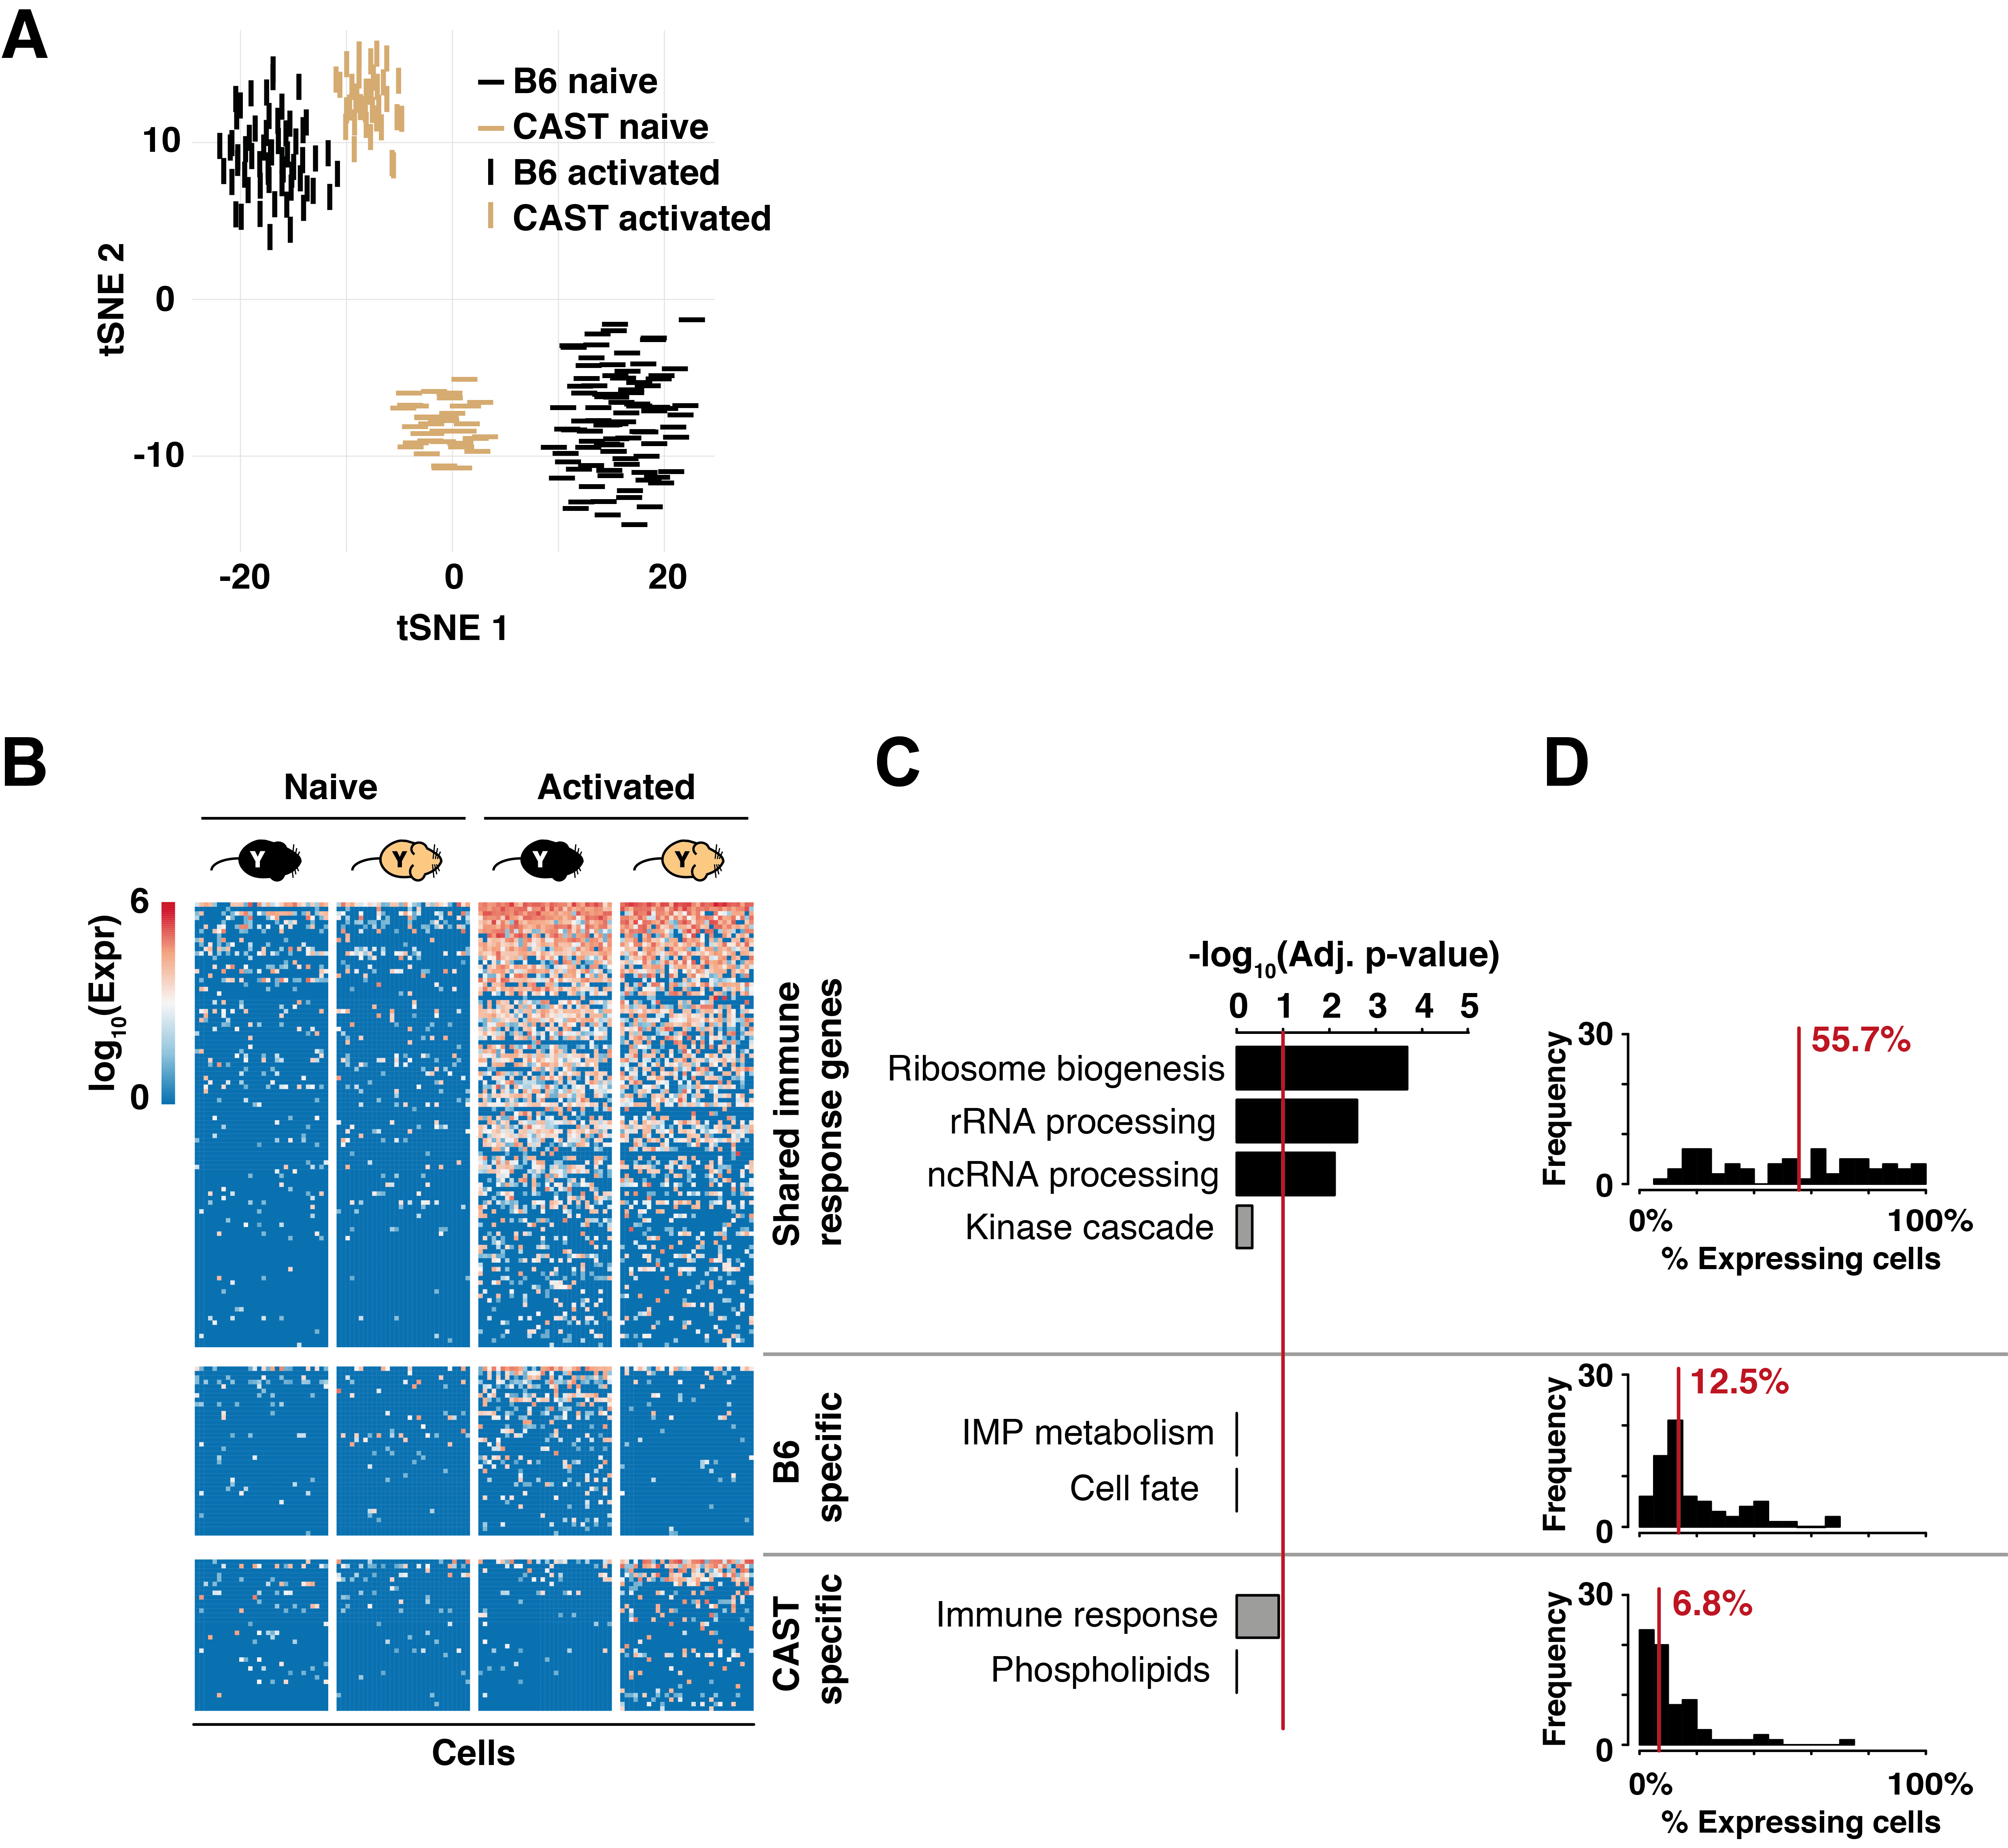
\includegraphics[width=\textwidth]{Fig_11.png}
\caption[X chromosome dynamics during spermatogenesis]{\textbf{X chromosome dynamics during spermatogenesis.} \\
\textbf{(A)} Schematic of sex chromosome sub-nuclear localisation through spermatogenesis, \textbf{(B)} For each cell, the ratio of mean expression of genes on Chr 9, Chr X and Chr Y to the mean expression of genes across all autosomes is represented as a boxplot for cells allocated to each developmental stage. SG – spermatogonia, M – metaphase, \textbf{(C)} Expression of all X chromosome genes (> 10 average counts) in bulk RNA-Seq data across the juvenile time course. Columns correspond to developmental stage and rows are ordered by the log$_2$ fold change between spermatocytes (stages before and including postnatal day (P) 20) and spermatids (stages after P20). Horizontal dashes indicate genes that are targets of \textit{Rnf8} (green) and \textit{Scml2} (blue) \citep{Adams2018}, \textbf{(D)} Average expression of spermatid-specific genes (panel (C)) per germ cell type. Columns are ordered by developmental stage and rows are ordered by peak gene expression through development. Multi-copy genes are highlighted in bold.}
\label{fig3:X_reactivation}
\end{figure}

\newpage

\section{Epigenetic mechanisms of X chromosome reactivation}

After identifying \emph{de novo} activated escape genes, we next profiled the epigenetic basis for such transcriptional dynamics. For this, we profiled the chromatin landscape in spermatocytes and spermatids using the newly developed CUT\&{}RUN protocol for low cell numbers \textbf{(Appendix \ref{appA.2})} \citep{Skene2018}. 

\subsection{CUT\&{}RUN to profile H3K4me3 and H3K9me3 marks}

In brief, from two individuals, we sorted spermatocytes and spermatids at P26 during the first wave of spermatogenesis \textbf{(Fig.~\ref{fig3:K9_global}A)}. At this stage, tubules contain spermatocytes close to the meiotic cell divisions and elongating spermatids. We assayed trimethylation of histone H3 on lysine 4 (H3K4me3) as a proxy for promoter activity, as well as repressive trimethylation of lysine 9 (H3K9me3). By profiling the enrichment of H3K9me3 across all chromosomes, we confirmed that the X chromosome has high levels of H3K9me3 in spermatids which has been previously shown \citep{Moretti2016, Greaves2006, Tachibana2007}. In addition, we now show that H3K9me3 accumulation begins earlier in meiosis, and indeed spermatocytes show enrichment of this repressive mark on the X chromosome \textbf{(Fig.~\ref{fig3:K9_global}B)}. \\

On autosomes, H3K9me3 is enriched in pericentromeric regions of constitutive heterochromatin \citep{Peters2001}. To assay the distribution of read pairs across whole chromosomes, we binned reads in 1kb windows across the chromosome. Next, we calculated the cumulative sum across 10,000 randomly sampled bins starting at windows with highest H3K9me3 enrichment. This measure indicates whether each window contains equal enrichment (slope is similar across the curve) or if some windows are enriched for the mark (slope decreases across the curve). As seen in \textbf{Fig.~\ref{fig3:K9_global}D}, the H3K9me3 enrichment appears to be homogeneously distributed across the X chromosome while, for example, the enrichment of the H3K9me3 mark on chromosome 9 is a lot more heterogeneous. \\

Nevertheless, when merging the 1000 windows with highest H3K9me3 enrichment, we detected broad regions showing particularly high levels of H3K9me3 scattered across the X chromosome \textbf{(Fig.~\ref{fig3:K9_global}C)}. Among the merged regions with highest H3K9me3 enrichment, we detect the promoter of \textit{Akap4}, a well-known escape gene. This discovery prompted us to profile the chromatin dynamics of active and repressive marks at promoters of \emph{de novo} escape genes (\emph{spermatid-specific genes}) versus the promoters of all other expressed X-chromosome genes (\emph{non-spermatid specific genes}) \textbf{(Fig.~\ref{fig3:X_reactivation}C)}.

\begin{figure}[!h]
\centering
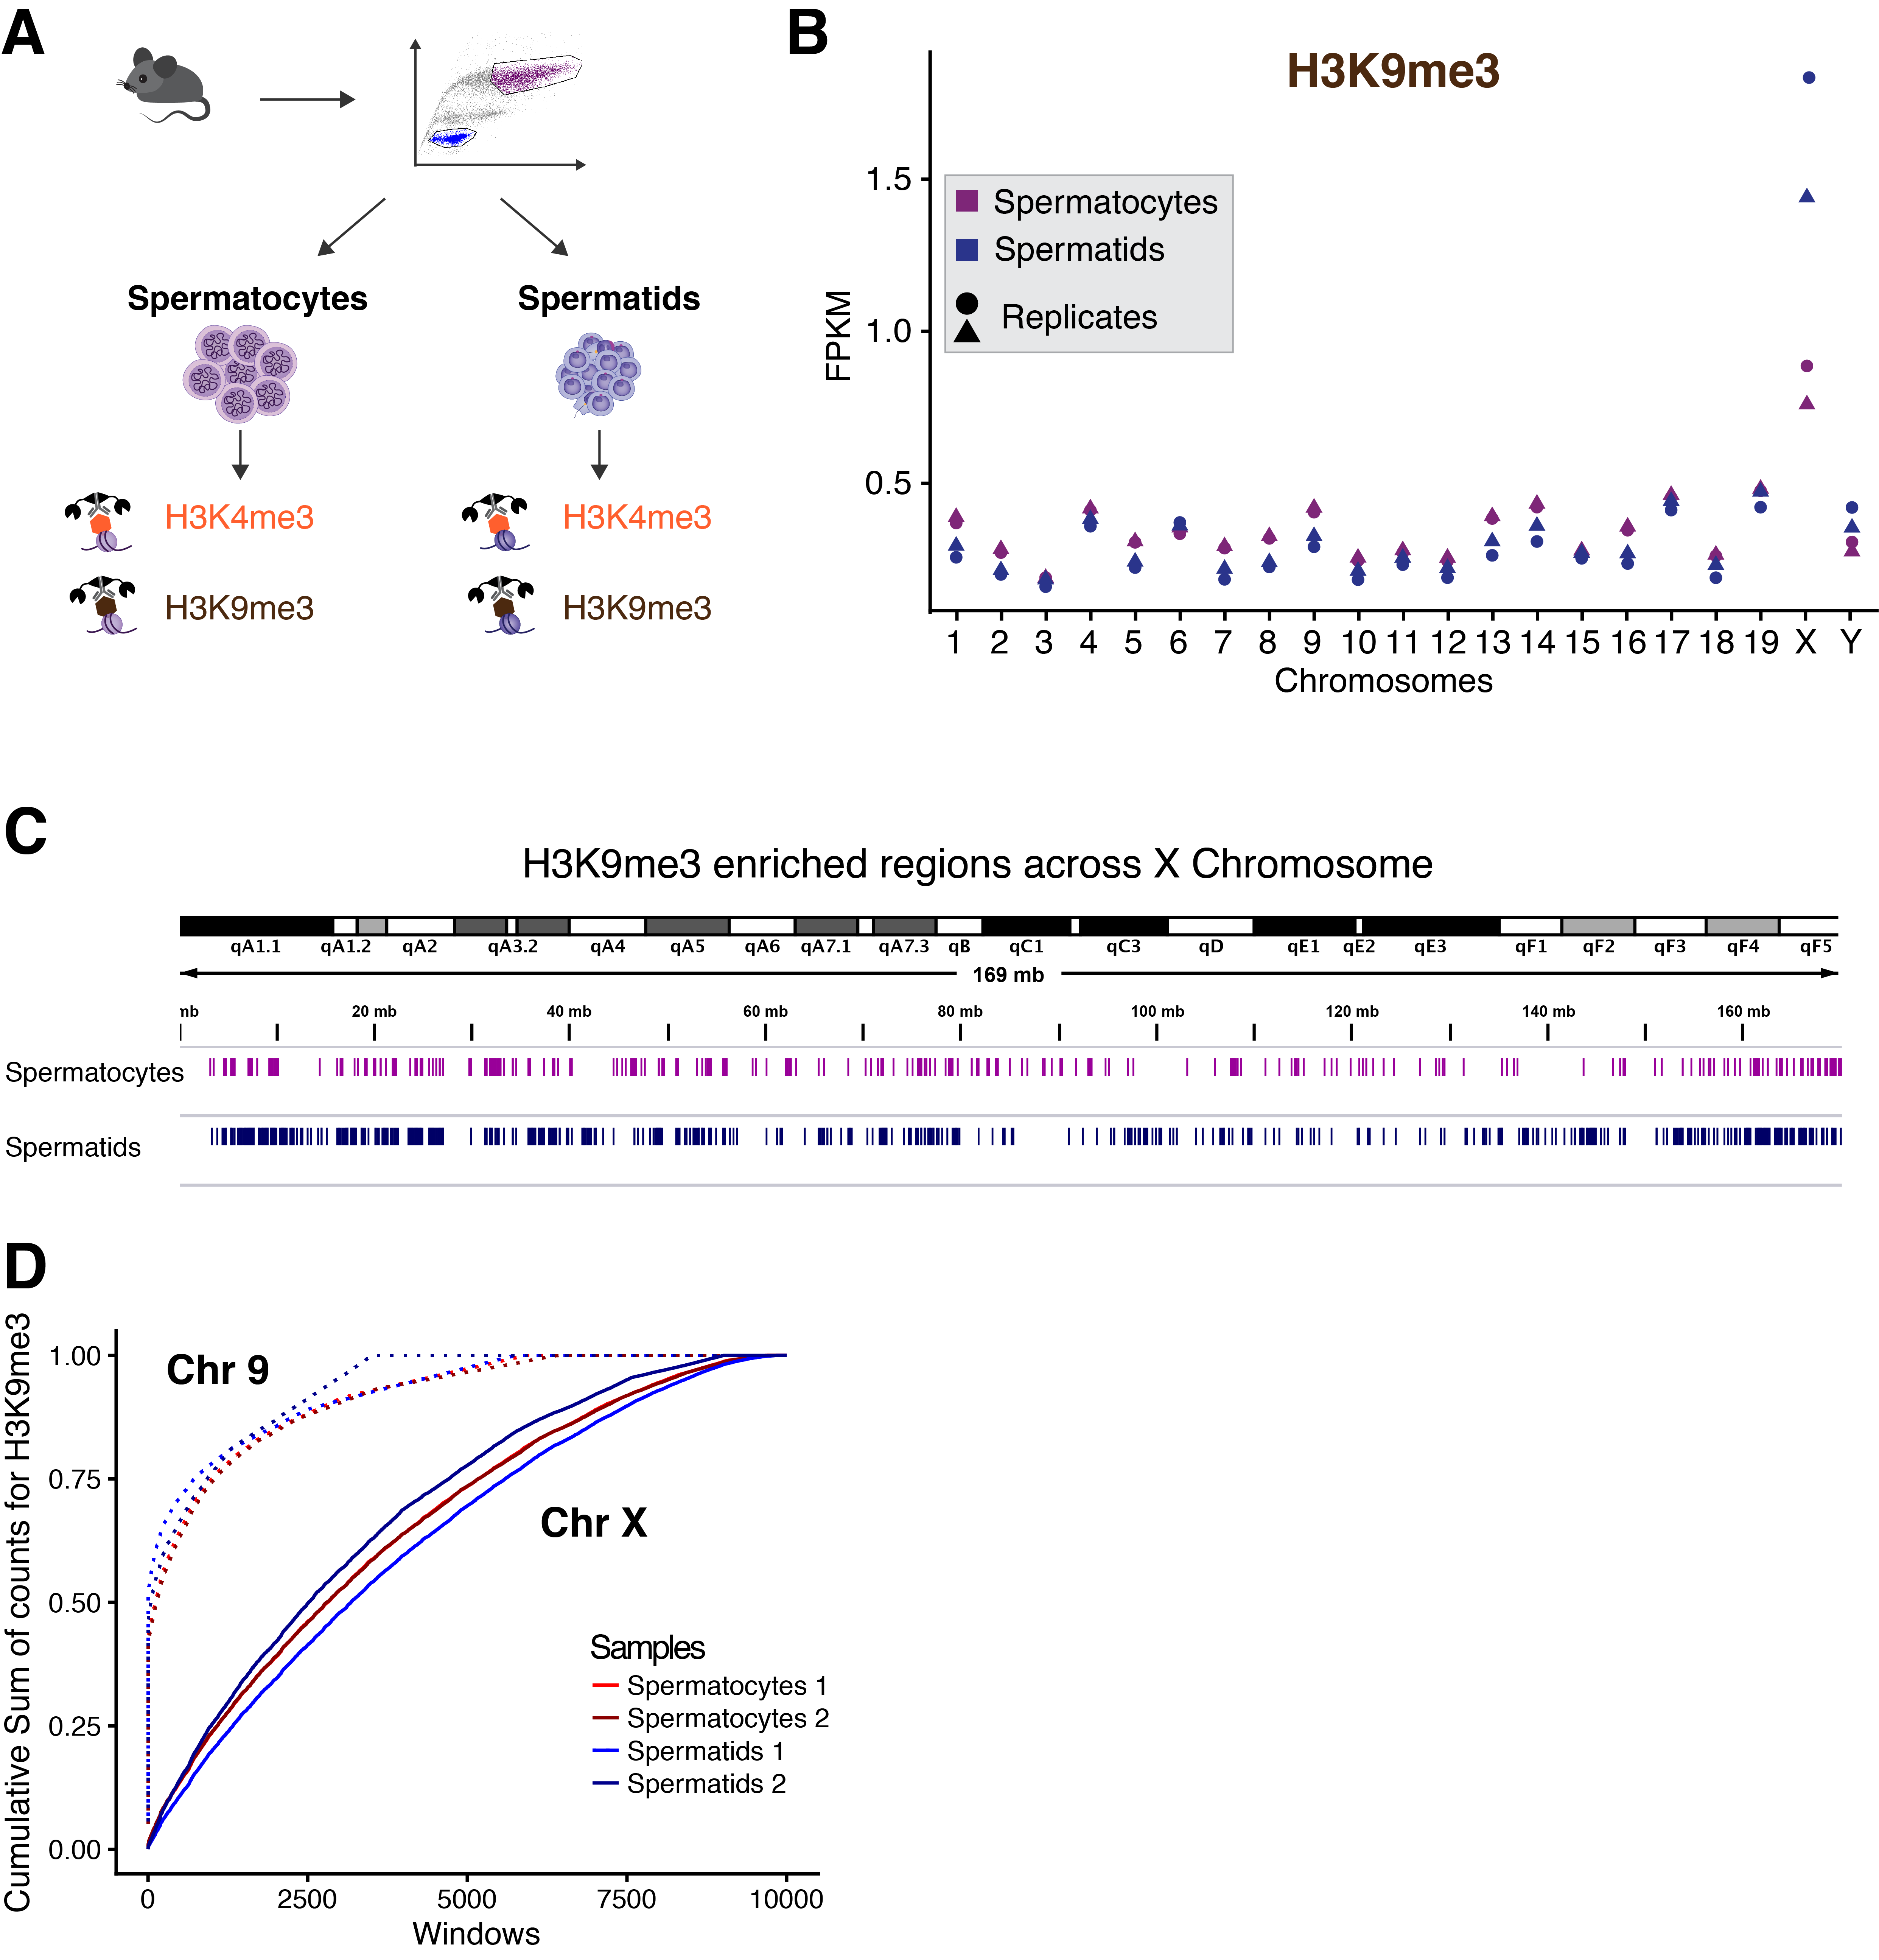
\includegraphics[width=\textwidth]{Fig_12.png}
\caption[Chromatin profiling in spermatocytes and spermatids]{\textbf{Chromatin profiling in spermatocytes and spermatids.} \\
\textbf{(A)} Spermatocytes and spermatids were isolated from the same individual using FACS and profiled using H3K4me3 (active mark) and H3K9me3 (repressive mark) using CUT\&{}RUN, \textbf{(B)} Number of H3K9me3 Fragments Per Kilobase per Million (FPKM) for each chromosome. Pink: spermatocytes, blue: spermatids. Shape corresponds to biological replicate, \textbf{(C)} The top 1000 windows with highest H3K9me3 signal (1000 bp width, CPM) were merged using a tolerance of 1500 bp. Representative tracks of one replicate in spermatocytes and one replicate in spermatids are shown, \textbf{(D)} Cumulative summed counts per million across 10000 randomly sampled windows (1000 bp width) visualizing the distribution of the H3K9me3 signal across chromosome 9 (dashed line) and chromosome X (solid line).}
\label{fig3:K9_global}
\end{figure}

\newpage

\subsection{Targeted silencing of spermatid-specific escape genes}

Here, we profiled the enrichment for H3K4me3 and H3K9me3 marks at promoters of spermatid-specific escape genes and all other X-linked genes in spermatides and spermatocytes. As a measure for enrichment, we calculated the Counts Per Million (CPM) for paired reads per promoter. In spermatocytes, spermatid-specific genes showed lower enrichment in H3K4me3 than non-spermatid specific genes (Wilcoxon-Mann-Whitney: p-value < 2.2x10$^{-16}$) \textbf{(Fig.~\ref{fig3:K9_K4_targeted}A, left panel)}. In contrast, spermatid-specific genes have on average elevated H3K4me3 in spermatids, as expected based on their increased expression level compared to spermatocytes \textbf{(Fig.~\ref{fig3:K9_K4_targeted}A, right panel)}. \\


When examining the deposition of H3K9me3 on the promoters of X-linked genes, we detected a strong enrichment in spermatid-specific escape genes in spermatocytes (Wilcoxon-Mann-Whitney: p-value < 3.7x10$^{-11}$) \textbf{(Fig.~\ref{fig3:K9_K4_targeted}B, left panel)}. This pattern indicates that spermatid-specific genes are more strongly repressed in spermatocytes. Due to the strong enrichment of H3K9me3 on the post-meiotic X chromosome, we detect similar H3K9me3 enrichment in promoters for both, spermatid-specific and non-specific X-linked genes \textbf{(Fig.~\ref{fig3:K9_K4_targeted}B, right panel)}.\\

Our results describe the precise epigenetic changes associated with escape gene activation in post-meiotic cells. These dynamics are exemplified by the chromatin remodelling that occurs around \textit{Akap4} and \textit{Cypt1}, both of which are well-studied spermatid-specific genes \textbf{(Fig.~\ref{fig3:K9_K4_targeted}C)}. The promoters of these genes have high levels of H3K9me3 in spermatocytes, which decreases in spermatids, while H3K4me3 levels are strongly increased. This targeted repression of a subset of X-linked escape genes could indicate a mechanism to repress otherwise lethal genes in spermatocytes that are later on needed in spermatid development. Examples of spermatocyte-lethal genes involved in spermatid development are two Y chromosome encoded genes: zinc finger protein Y-linked (\textit{Zfy}) 1 and 2 \citep{Royo2010}.

\newpage

\begin{figure}[!h]
\centering
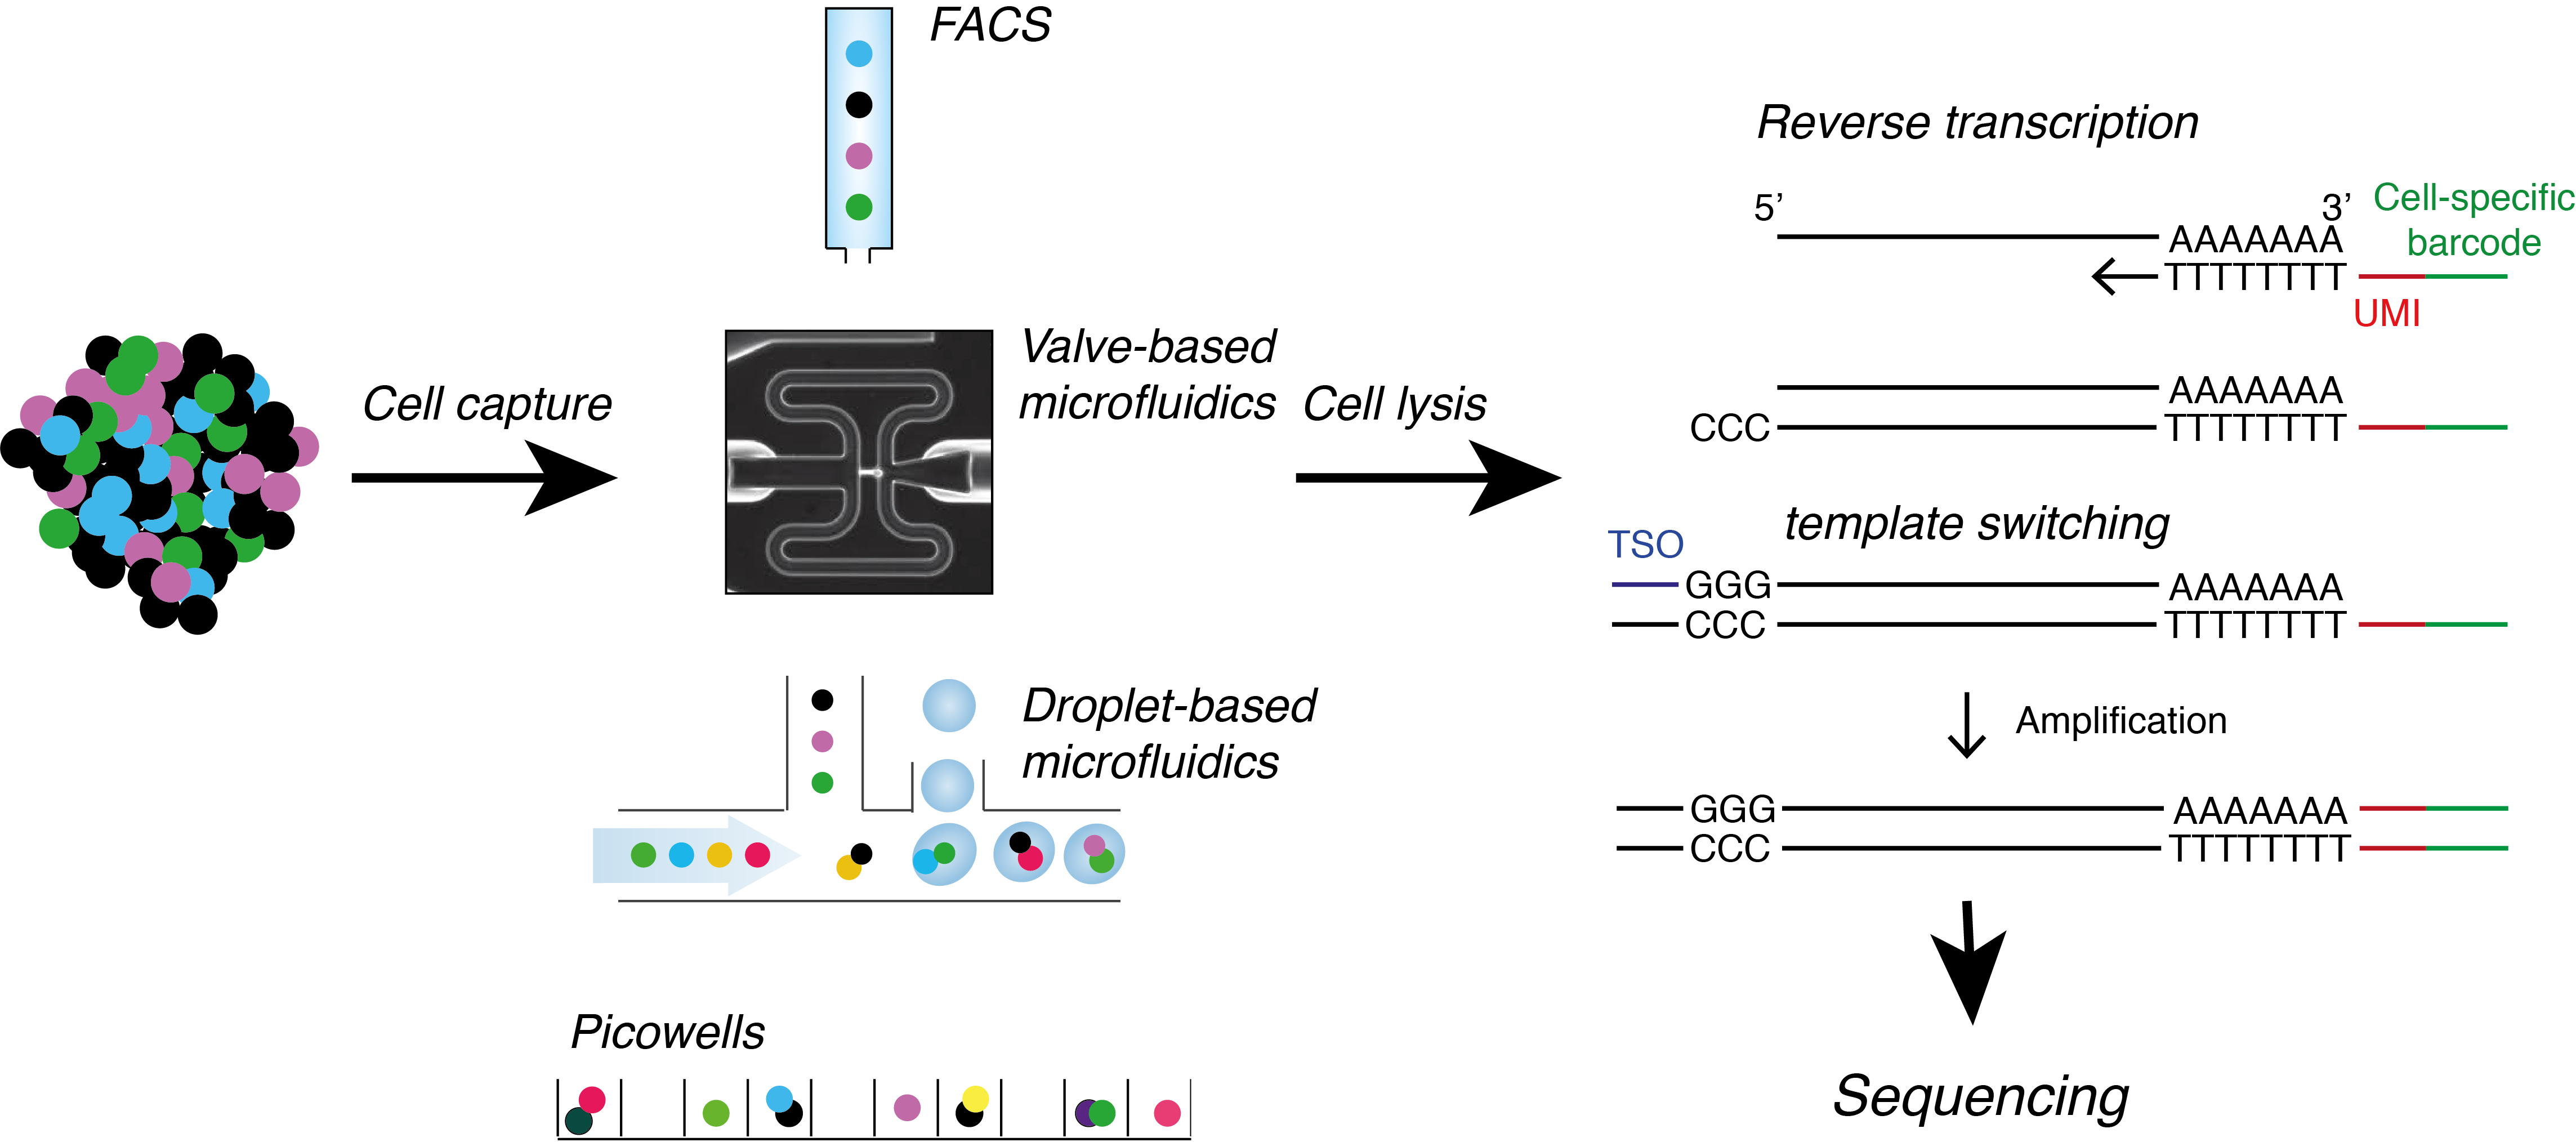
\includegraphics[width=\textwidth]{Fig_13.png}
\caption[Targeted repression of spermatid-specifc escape genes in spermatocytes]{\textbf{Targeted repression of spermatid-specifc escape genes in spermatocytes.} \\
\textbf{(A)} and \textbf{(B)} Boxplot of H3K4me3 (A) and H3K9me3 (B) Counts Per Million (CPM) in promoter regions of spermatid specific (n=127) and non-spermatid specific (n=617) genes for spermatocytes (left) and spermatids (right).  \# indicates statistical significance (Wilcoxon-Mann-Whitney: p-value < 1x10$^{-10}$), n.s. – not significant, 
\textbf{(C)} Genome tracks of H3K4me3 and H3K9me3 for two representative spermatid-specific genes (\textit{Akap4} and \textit{Cypt1}) for spermatocytes (left) and spermatids (right). Reads were scaled by library size. The genomic location of these genes is indicated below the tracks where exons are labelled as blocks and the directionality of transcription is shown by arrows.}
\label{fig3:K9_K4_targeted}
\end{figure}

\newpage

\section{Measuring changes in variability over pseudo-time}

As described above, spermatogenesis is a unidirectional and continuous differentiation process coupled to a complex system of developmental steps. I next asked whether this differentiation process is coupled to changes in transcriptional variability. In mouse hematopoietic cell differentiation, cell-to-cell diversity increases at critical state transitions where cell fate decisions are made \citep{Mojtahedi2016}. A similar effect was detected in chicken erythroid progenitor cells where the Shannon entropy is highest directly at the point of fate commitment and declines upon the irreversible commitment to differentiation \cite{Richard2016}. In the previous chapter, we have demonstrated that transcriptional variability shows dynamic changes during CD4\plus{} T cell differentiation with high variability being observed at a possible early commitment point and a decrease in variability upon proliferation. In this section, I applied the regression BASiCS model which was developed in the previous chapter to study changes in transcriptional variability over the time-course of spermatogenesis. More specifically, I profiled changes in variability for individual genes during spermiogenesis, the differentiation process that directly follows meiosis (see \textbf{Section \ref{sec3:spermiogenesis}}). As described above, spermiogenesis is a differentiation process that involves an extensive remodelling of the chromatin with transcriptional shut-down occurring at around spermatid stage S10. Modelling changes in expression over a differentiation time-course is done by ordering transcriptional profiles of individual cells along their so called \emph{pseudo-time}. Different methods have been proposed to perform this ordering based on minimum spanning trees \citep{Trapnell2014} and nearest-neighbour graphs \cite{Setty2016}, Gaussian Processes \citep{Reid2016a, Campbell2016b} and diffusion maps \citep{Haghverdi2016}. Once the pseudo-temporal ordering is determined, genes which change in expression over pseudo-time can be found by fitting a generalized linear model to the expression counts and performing a likelihood ratio test against a null model with no pseudo-time dependence \citep{Trapnell2014}. Profiling changes in variability is more complicated as single-cell measures of variability are not available. 

\subsection{Using BASiCS on continuous data}

Here, I use BASiCS to estimate residual over-dispersion parameters for homogeneous cell populations along the differentiation time-course. Different approaches of identifying homogeneous populations exist. First, ordered cells can be split into populations of equal size (e.g.~200 cells per group). This approach produces heterogeneous cell populations when cell state transitions occur within the population. I therefore rely on the clustering performed in \textbf{Section \ref{sec3:clustering}} which splits the full cell population along the differentiation trajectory. For each cluster from S1 to S14, the regression BASiCS model was run for 40,000 iterations with 20,000 iterations burn-in and a thinning value of 20. 

\newpage

For each gene in each of the 14 spermatid populations, BASiCS generates a posterior distribution estimating the residual over-dispersion parameter in form of an MCMC chain \textbf{(Fig.~\ref{fig3:variability_schematic}A)}. These measures are independent of mean expression (see previous chapter) and can therefore be used to study changes in variability which are not confounded by changes in mean expression throughout the differentiation of sperm. To profile and test temporal changes of transcriptional variability during spermiogenesis, I choose two approaches. \\

First, I used iterative fitting of a linear regression between the residual over-dispersion parameters and the progression of spermiogenesis to find linear changes in variability. For this, I selected spermatids from stages S1 to S9 prior to transcriptional shut-down. Transcriptional changes after S10 are only due to degradation of mRNA and I assume that linear changes in variability occur before S10. In more detail, for each MCMC iteration, I fit a linear regression between the current samples of $\epsilon_i$ against the cluster label \textbf{(Fig.~\ref{fig3:variability_schematic}B)}. This fitting is performed for each gene individually and generates a \emph{post hoc} distribution of the intercept and the slope regression coefficient that captures uncertainty in the regression fit. Focusing on the slope coefficient, I can compute the posterior tail probability of the slope coefficient being different from 0. If the posterior tail probability is larger than a threshold (e.g.~80\%), I consider the transcriptional variability of this gene to be either positively or negatively associated with temporal ordering depending on the sign of the median slope coefficient \textbf{(Fig.~\ref{fig3:variability_schematic}B)}. Similar to differential testing described in the previous chapter, the probability threshold is determined by fixing the expected false discovery rate to 10\%. A similar testing can be done for the slope coefficient when fitting a linear model between the group wise mean expression parameter $\log(\mu_i)$ and the group labels.\\

Secondly, to detect non-linear patterns of changes in transcriptional variability, I perform clustering on the gene-specific variability profiles across spermatid populations S1-S14. Similar approaches have been chosen to find patterns of genes expression across pseudo-time. Common patterns for changes in expression levels include immediate, transient and gradual up- or down-regulation \citep{Trapnell2014}. When profiling changes in variability over the time-course of differentiation these clustered profiles can indicate similarly strong or weak transcriptional regulation or similar expression rates \textbf{(Fig.~\ref{fig3:variability_schematic}C)}.

\newpage

\begin{figure}[!h]
\centering
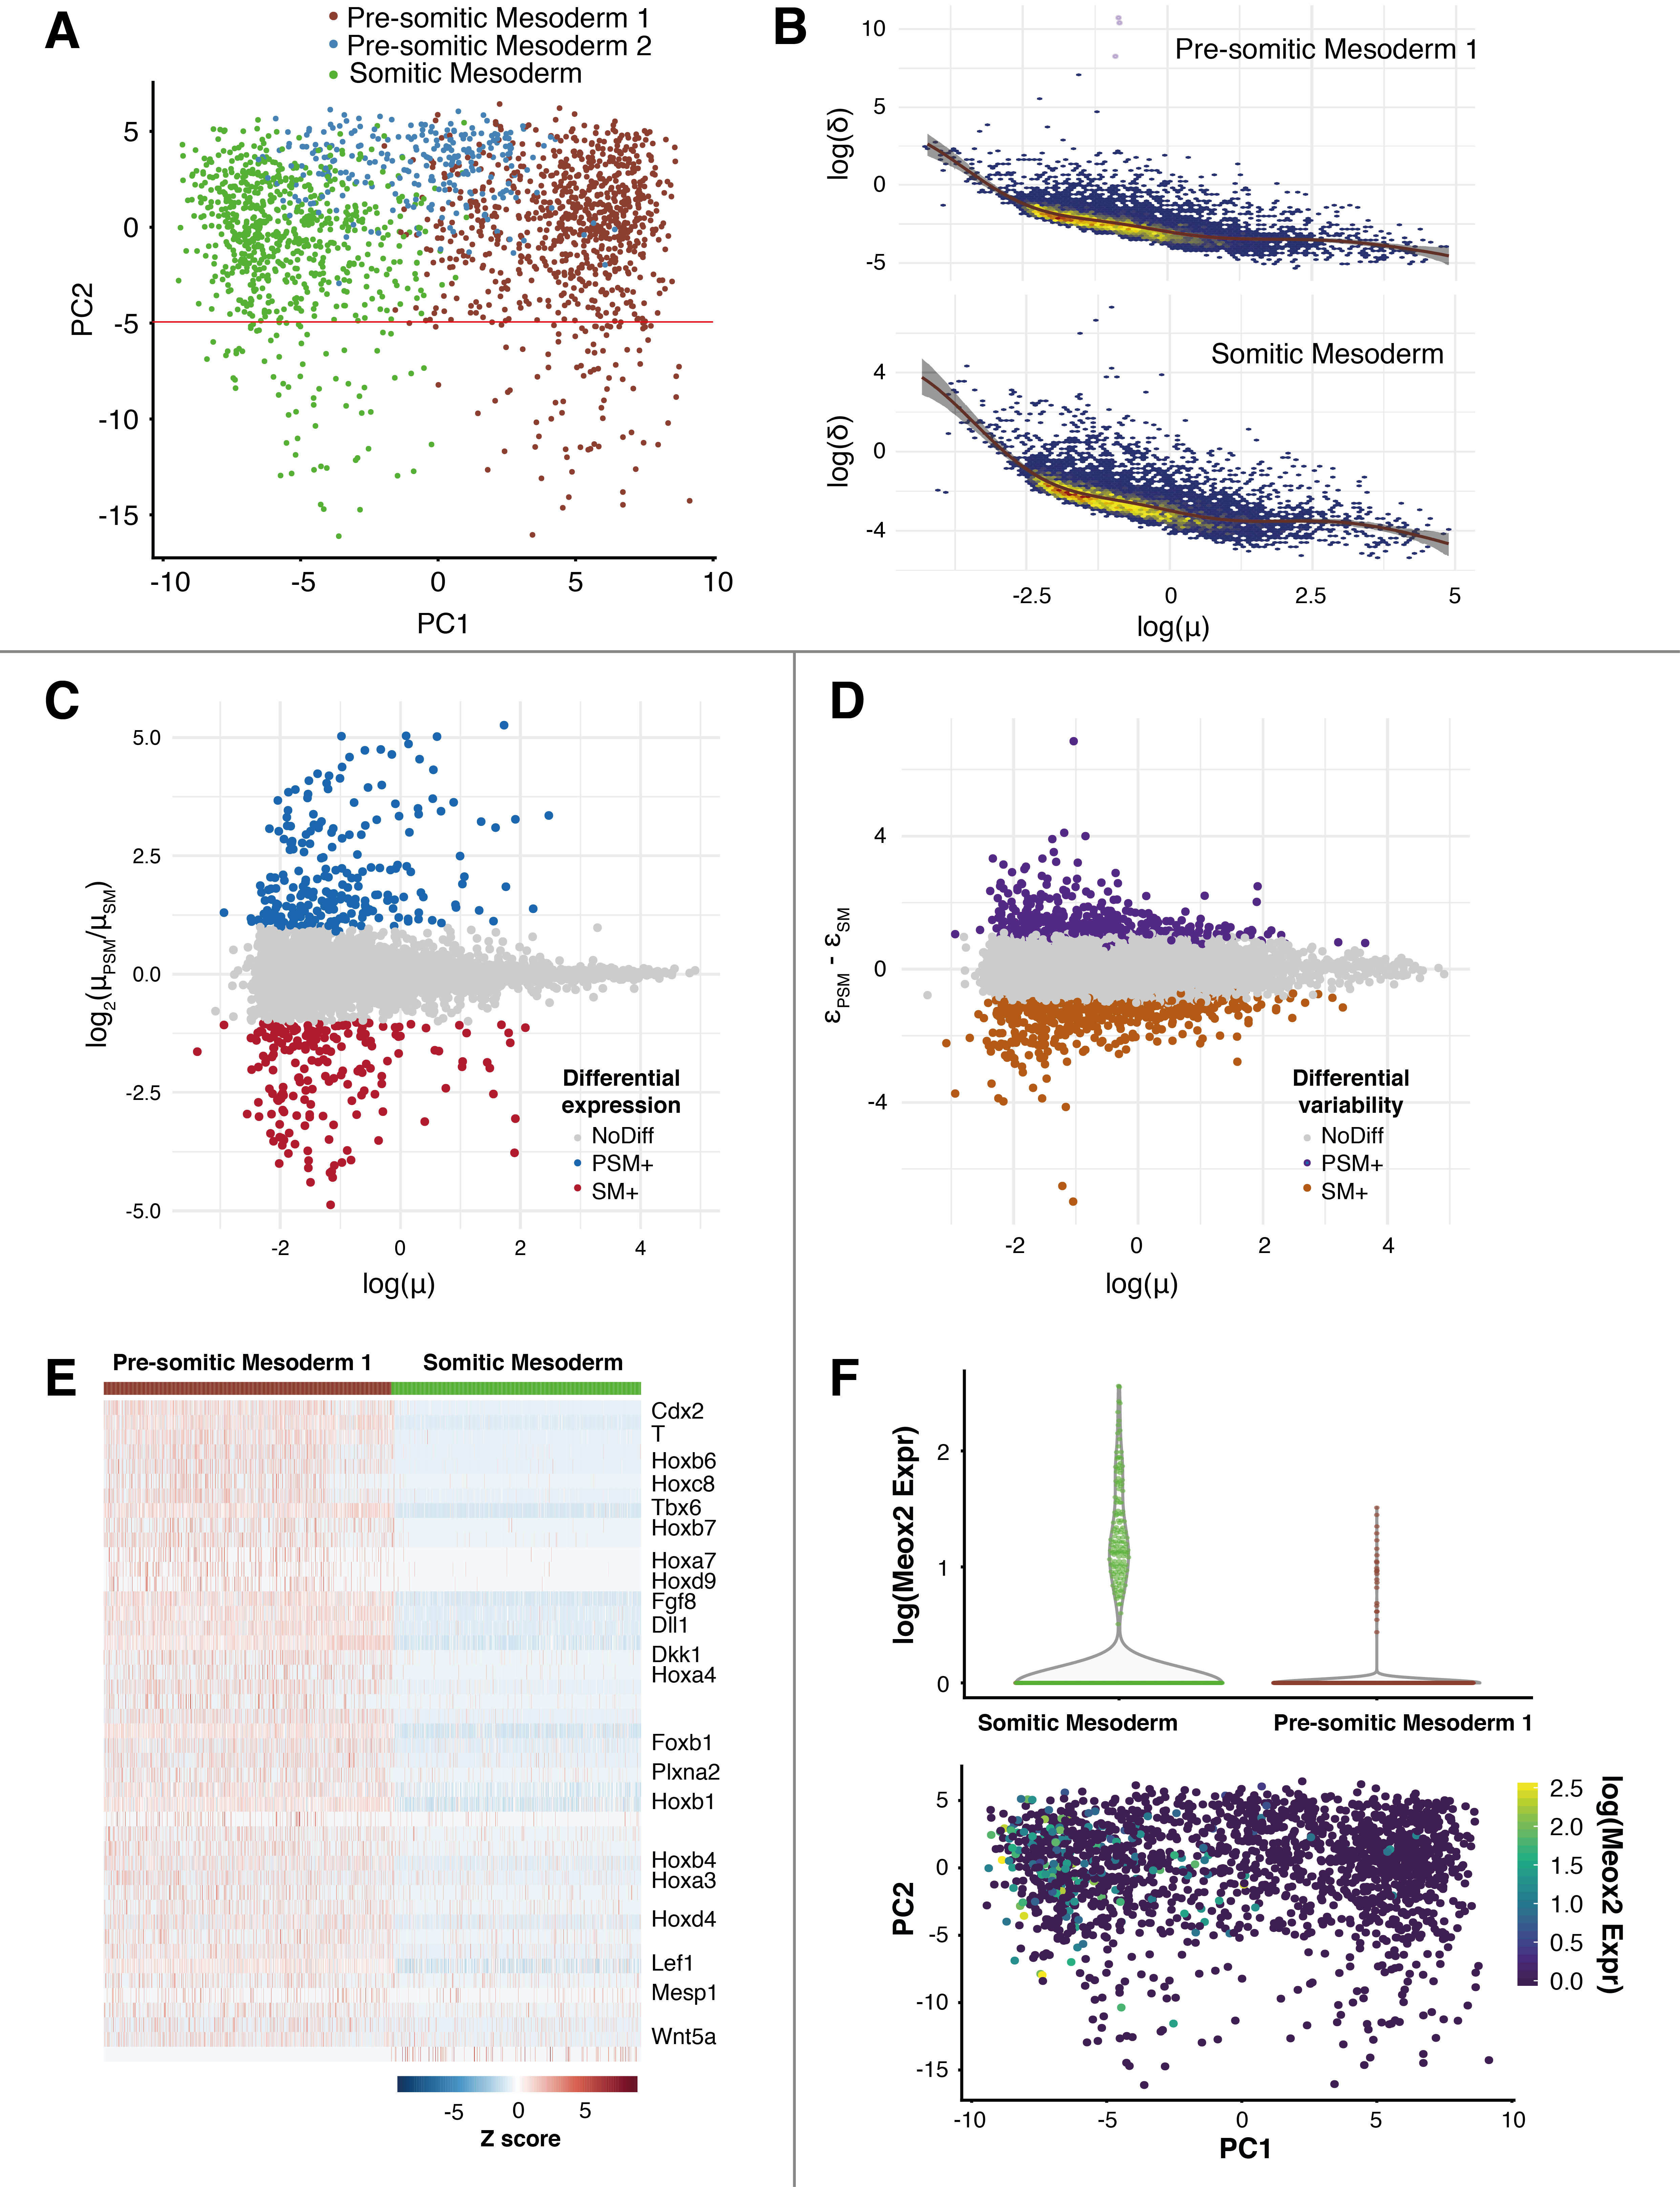
\includegraphics[width=0.8\textwidth]{Fig_14.png}
\caption[Detecting changes in variability over pseudo-time]{\textbf{Detecting changes in variability over pseudo-time.}\\
\textbf{(A)} For each group of spermatid, BASiCS  generates a posterior distribution of residual over-dispersion parameters $\epsilon_i$. Cell groups can be ordered based on their pseudo-time (upper panel). Lower panels indicate the MCMC chain for gene-specific $\epsilon_i$ per group (A, B, ..., X), \textbf{(B)} For each iteration of the MCMC (1,...,n), a linear regression was fit between the current samples of $\epsilon_i$ against the group labels for spermatids (S) 1-9. This approach generates a \emph{post hoc} distribution of the slope coefficient $\beta_1$ (lower panels). The distribution is used to calculate the posterior probability of observing $\beta_1\neq0$, \textbf{(C)} Clustering was performed on variability profiles across spermatid populations S1 to S14. A smooth regression (loess) was fit to $\epsilon_i$'s of the genes within each cluster. Genes that quickly decrease in variability (left panel), increase then decrease in variability (middle panel) or quickly increase in variability (right panel) can be identified.}
\label{fig3:variability_schematic}
\end{figure}

\newpage

\subsection{Finding continuous changes in variability by linear model fitting}

To detect single genes that continuously increase of decrease in variability, I fit a linear regression to each iteration of the MCMCs sampling $\epsilon_i$ or $\mu_i$ \emph{versus} the group labels \textbf{(Fig.~\ref{fig3:variability_schematic}B)}. The posterior distributions of the slope coefficient were used to categorise genes based on their transcription dynamics along the differentiation time-course (middle panel in \textbf{Fig.~\ref{fig3:linear_variability}}). These categories include: 

\begin{itemize}
\itemsep0em 
\item Increase in mean expression, no change in variability
\item Increase in mean expression, increase in variability
\item Increase in mean expression, decrease in variability
\item Decrease in mean expression, no change in variability
\item Decrease in mean expression, increase in variability
\item Decrease in mean expression, decrease in variability
\item No change in mean expression, no change in variability
\item No change in mean expression, increase in variability
\item No change in mean expression, decrease in variability
\end{itemize}

This approach leads to the detection of few genes that significantly change in variability over the differentiation time-course in a linear fashion while the majority of genes change only in mean expression. One hypothesis is that sperm maturation is a tightly regulated progress where the majority of genes follow a clear transcriptional pattern. Such a process contrasts other differentiation programmes such as hematopoiesis where branching events occur and the whole cell population expands in transcriptional variability to find new attractor states \citep{Mojtahedi2016}. To visualize changes in transcriptional variability, I selected representative genes from four categories: (i) Increase in mean expression, increase in variability, (ii) Increase in mean expression, decrease in variability (iii) Decrease in mean expression, increase in variability, (iv) Decrease in mean expression, decrease in variability (see inlets in \textbf{Fig.~\ref{fig3:linear_variability}}). Interestingly, \textit{Tsga8}, one of the most rapidly evolving X-linked genes, shows a strong increase in expression and a clear decrease in transcriptional variability. \emph{Tsga8} has been reported to be involved in hybrid sterility where F$_1$ crosses of mice form different strains are unable to reproduce. This effect might be due to the strong divergence of the \emph{Tsga8} sequence between species \citep{Good2011}. A tight regulation of its expression during spermiogenesis can therefore further control the phenotypic effect in F$_1$ animals.

\newpage

\begin{figure}[!h]
\centering
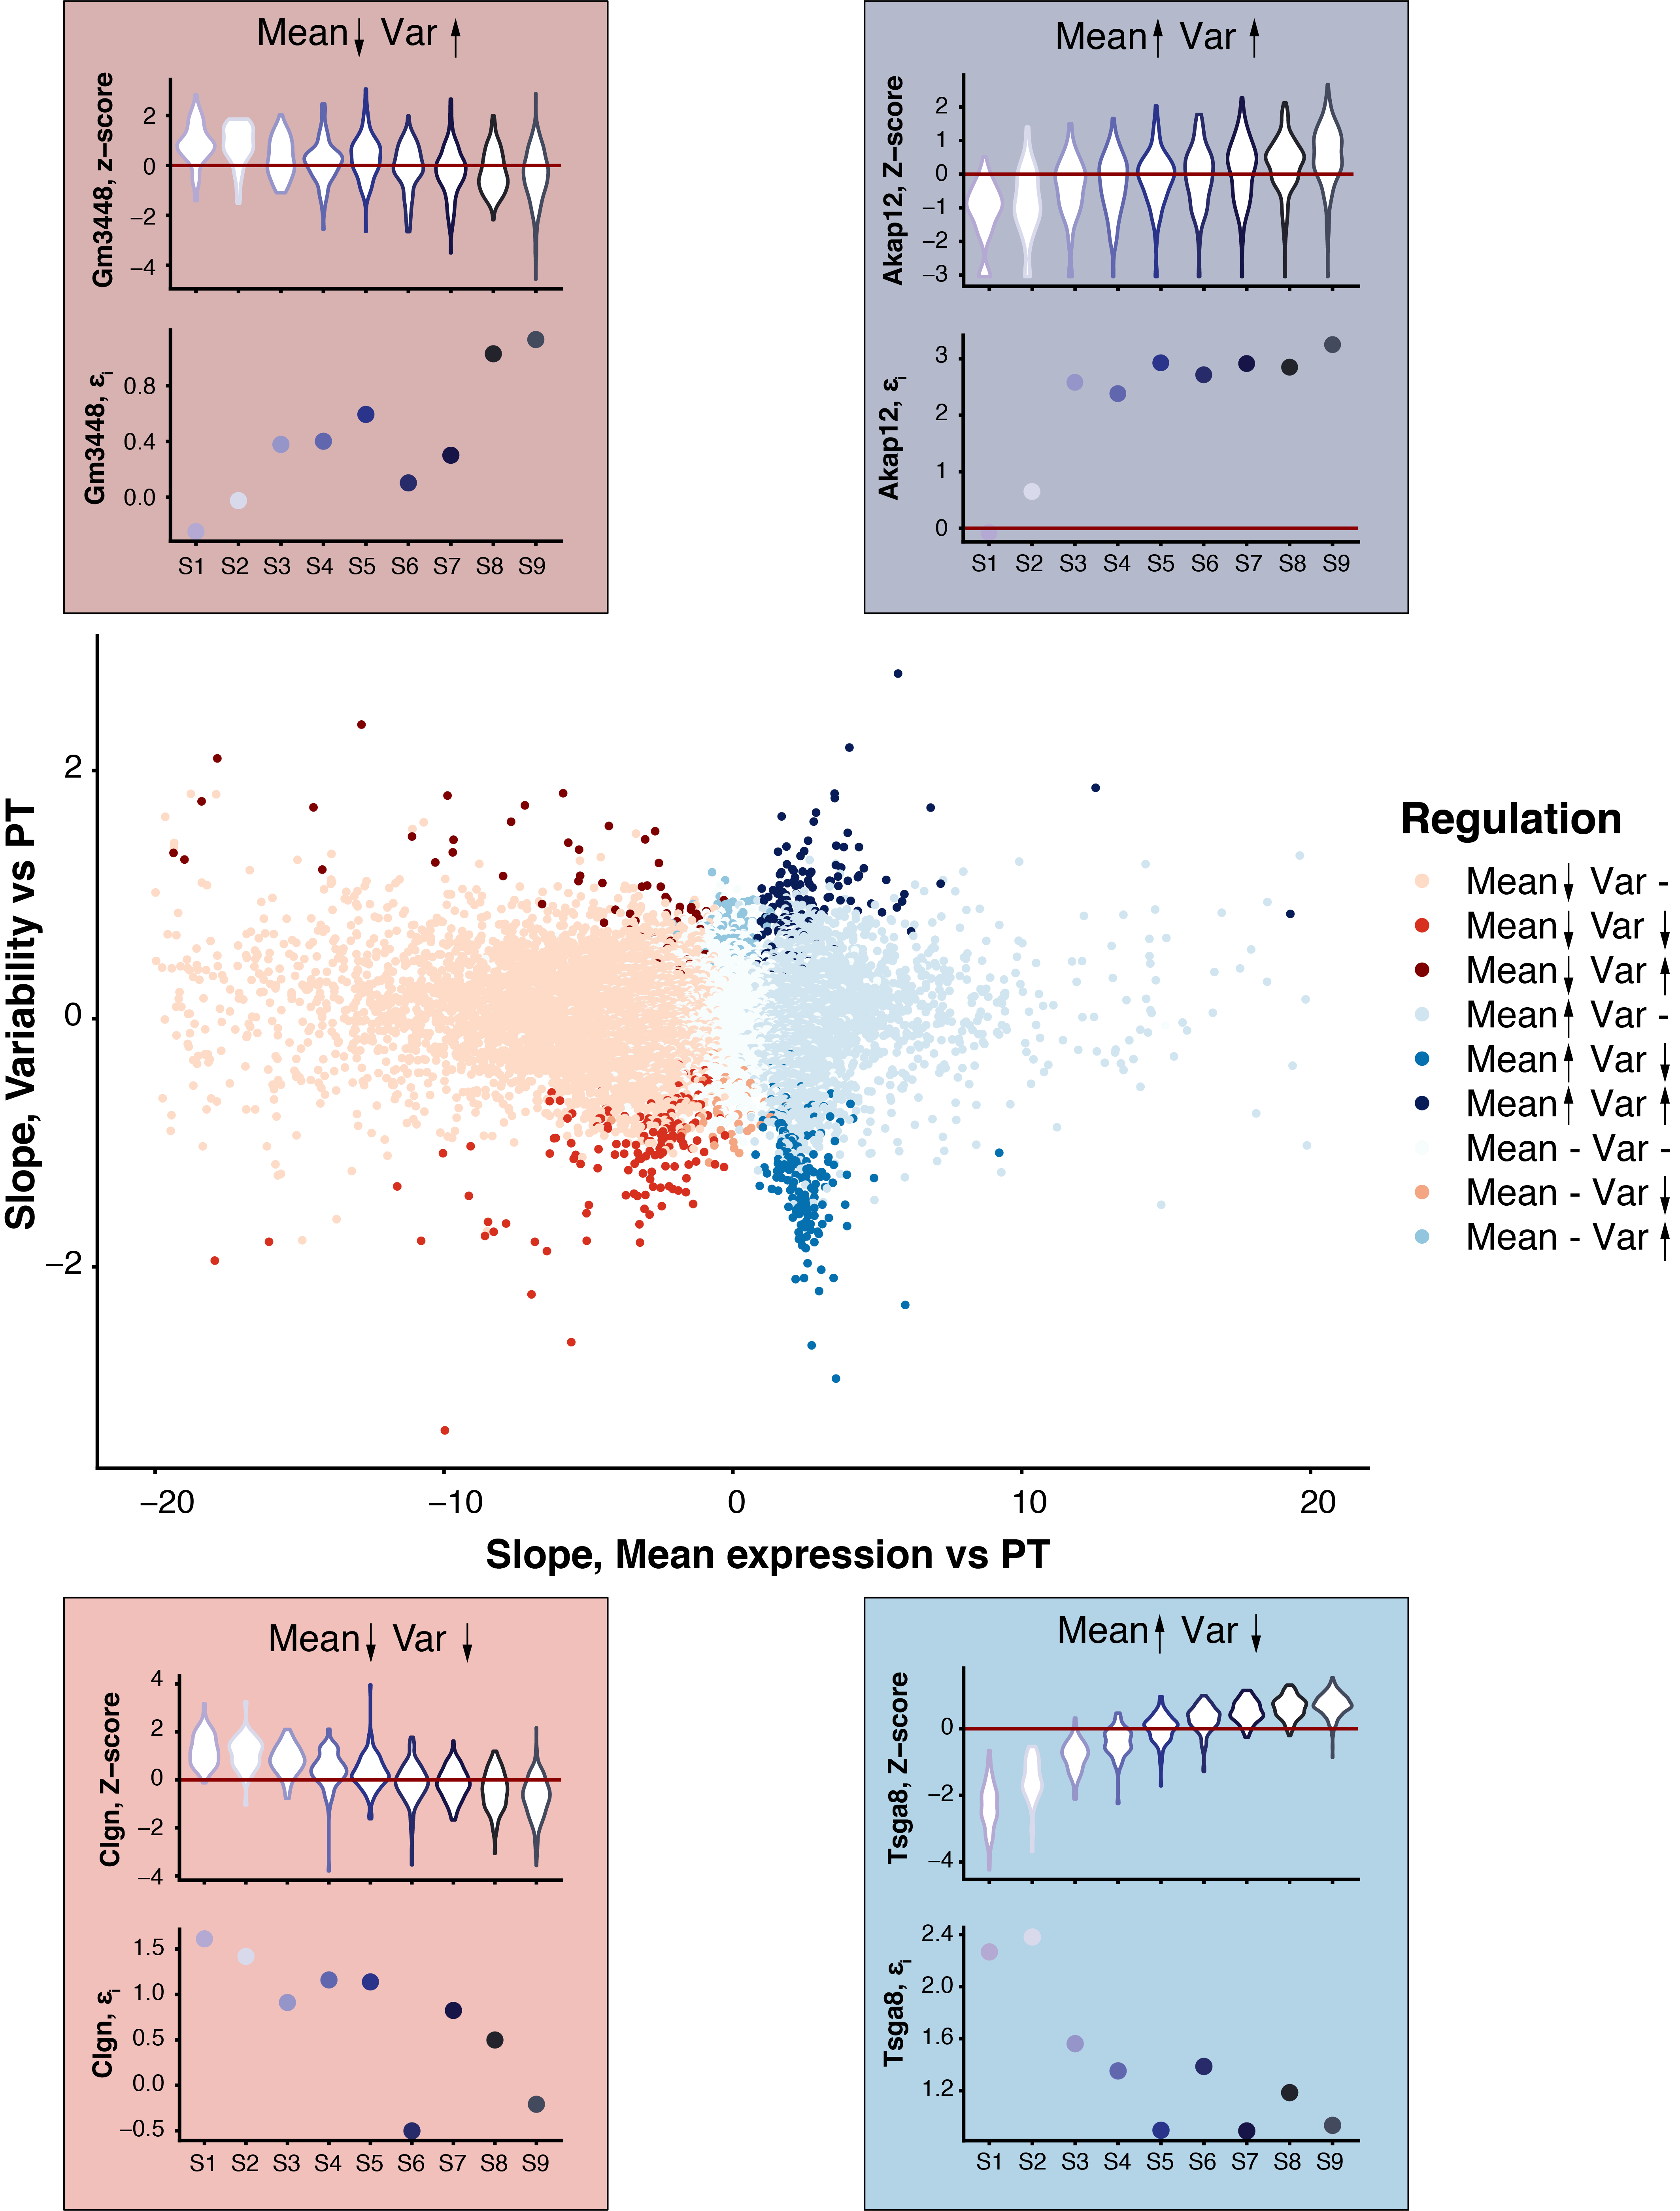
\includegraphics[width=0.8\textwidth]{Fig_15.png}
\caption[Linear changes in variability over spermiogenesis]{\textbf{Linear changes in variability over spermiogenesis.}\\
Linear models were fit between the residual over-dispersion parameter $\epsilon_i$ or the mean expression parameter $\mu_i$ and the groups labels (S) 1-14 for each iteration of the MCMC. Median posterior estimates of the slope parameter of the variability fit were plotted against the slope parameter of the mean expression fit. each dot represents a single gene. Genese are coloured based on their regulation (legend). Plot inlets indicated the Z score scaled normalized expression (upper panel) and the group-wise residual over-dispersion estimates $\epsilon_i$ (lower panels) of representative genes for four categories.}
\label{fig3:linear_variability}
\end{figure}

\newpage

\subsection{Clustering of variability profiles}

To identify non-linear patterns across all genes, I first ordered variability profiles based on their peak in variability \textbf{(Fig.~\ref{fig3:variability_clustering}A)}. Here, variability profiles are represented by the median residual over-dispersion parameter $\epsilon_i$  ordered from S1 to S14. Most variability profiles showed highest variability in specifically one group while also other patterns of variability are detectable. \\

To identify the major patterns of variability across the full range of spermiogenesis, I performed k-means clustering across all variability profiles. In this case, I had to select the expected number of clusters. Due to the fact that most genes showed peak variability in exactly one group, I selected $\text{k}=20$ to detect patterns other than peaks in single groups. After clustering, I detect a variety of variability patterns ranging from high variability in early spermiogenesis to high variability at later stages \textbf{(Fig.~\ref{fig3:variability_clustering}B)}. Most interestingly, I observed patterns that show gradual increase in variability until around spermatid stage S9 and decrease afterwards \textbf{(Fig.~\ref{fig3:variability_clustering}B, middle panel)}. \\

The group with peak variability at around S9 consists of all transition proteins (\textit{Tnp1}, \textit{Tnp2}) and protamins (\textit{Prm1}, \textit{Prm2}, \textit{Prm3}). When visualizing the expression patterns of \textit{Prm1}, I detect a quick shift in expression within cells from S9 \textbf{(Fig.~\ref{fig3:variability_clustering}C, middle panel)}. Similarly, genes that show highest variability at later stages during spermiogenesis \textbf{(Fig.~\ref{fig3:variability_clustering}B, second to last panel)} show a quick transcriptional decline after transcriptional shut-down (e.g.~ \emph{Tekt4}, \textbf{Fig.~\ref{fig3:variability_clustering}B}). \\

These results indicate that the changes in expression associated to the trajectory of pseudo-time are additional confounding factors when quantifying transcriptional variability. Similar to removing the confounding between mean expression and variability, a regression approach can be chosen to correct variability measures based on the correlation between expression and pseudo-time. 



\newpage

\begin{figure}[!h]
\centering
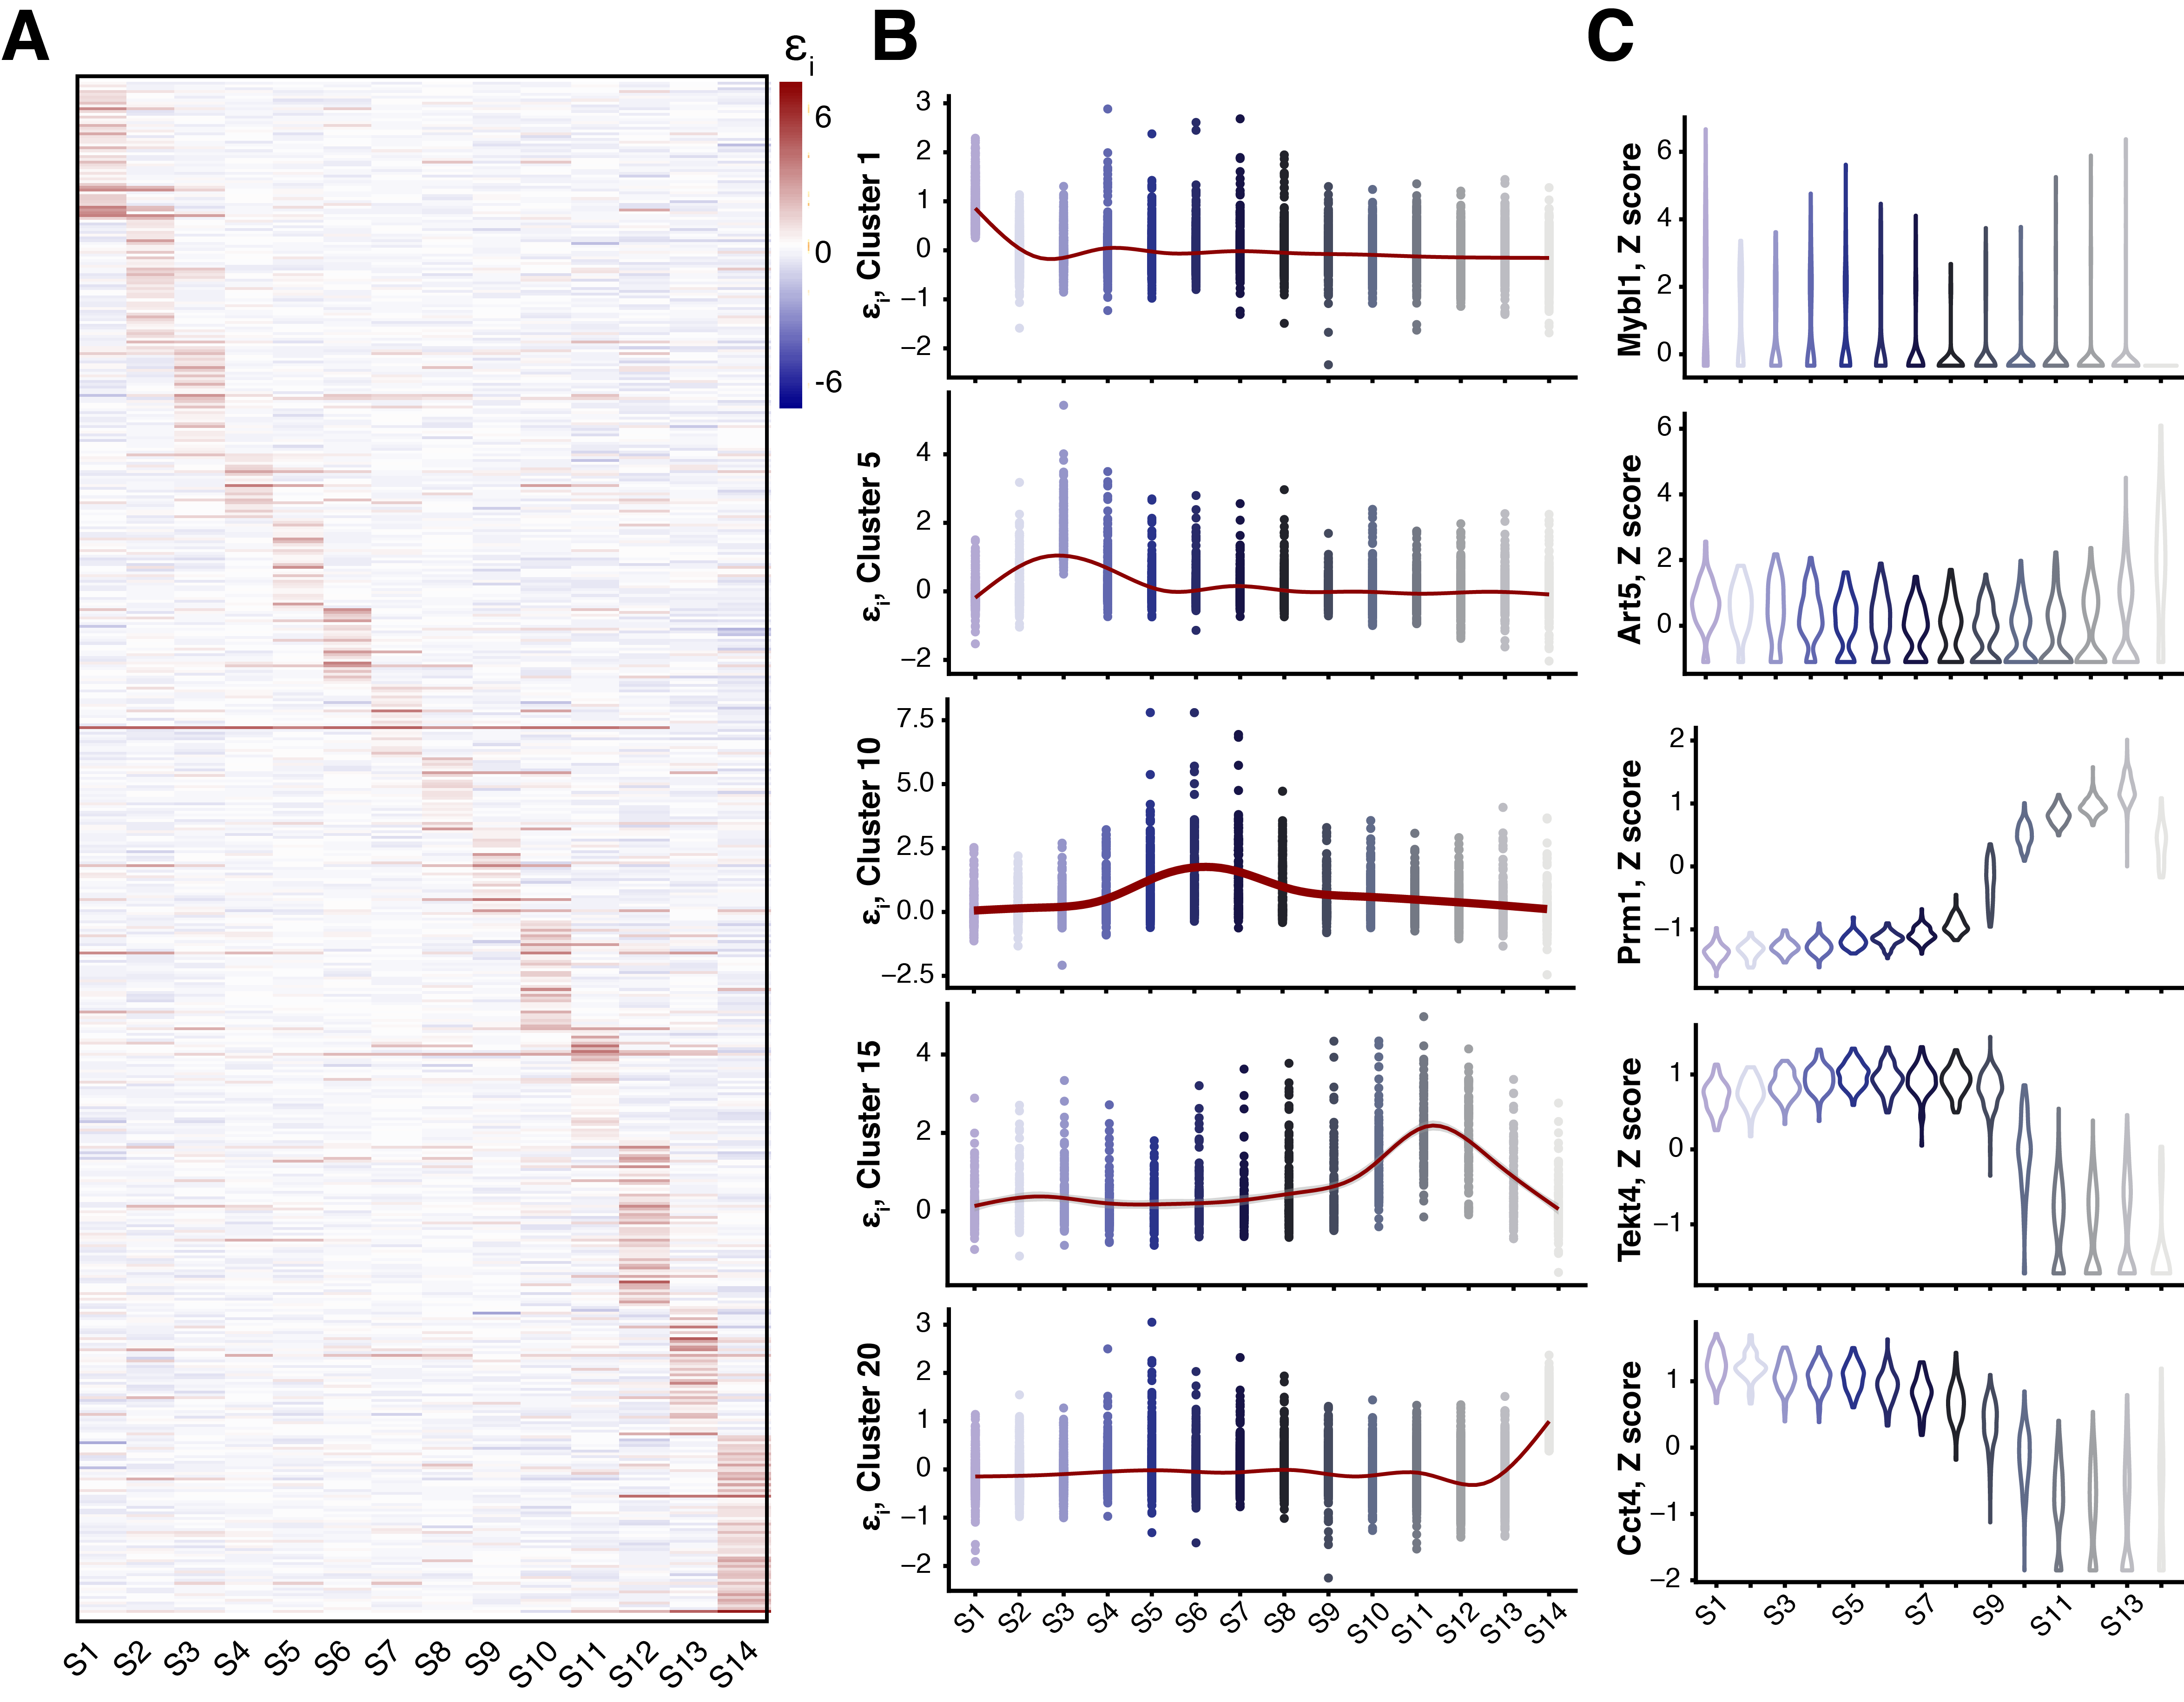
\includegraphics[width=\textwidth]{Fig_16.png}
\caption[Clustering of variability profiles]{\textbf{Clustering of variability profiles.}\\
\textbf{(A)} Variability profiles (median of the $\epsilon_i$ estimates ordered by developmental progression) were ordered based on their maximum $\epsilon_i$ starting in S1 spermatids, \textbf{(B)} Variability profiles were clustered using k-means with $\text{k}=20$. 5 representative patterns of variability are displayed ranging from highest variability in round spermatids to highest variability in elongating spermatids, \textbf{(C)} Z score scaled, normalized expression of example genes per variability pattern taken from (B) are displayed in form of boxplots.}
\label{fig3:variability_clustering}
\end{figure}

\newpage
%!TEX root = ../chapter3.tex
%******************************
%	 Discussion 
%*****************************

\section{Discussion}

The testes are among the most proliferative tissues in the adult body and ensure fertility via the continuous production of millions of sperm per day. Most developmental differentiation processes require the profiling of cellular populations at several time points \citep{Kernfeld2018, Scialdone2016, Wagner2018}. One of the exemptions is blood formation where commitment to different lineages can be profiled at once \citep{Dahlin2018}. Similarly, spermatogenesis occurs in continuous waves throughout the reproductive life span of animals. At any given time-point, all intermediate cell-types that arise across the ~35 day differentiation program are present in adult testes. This provided a powerful opportunity to capture and profile an entire differentiation process by profiling the transcriptomes of thousands of single-cells at a single time point. \\

We exploited the natural synchronisation of the first wave of spermatogenesis to identify key developmental transitions within the differentiation trajectory. Because germ cells have only progressed to a defined developmental point, the differentiation trajectory was truncated, facilitating identification of the most mature cell type.
In contrast, Chen \emph{et al.}, 2018 sorted synchronised spermatocyte and spermatid populations after blocking spermatogenesis with WIN 18,446. This allowed a strict enrichment for cells in specific stages during spermatogenesis but lost the natural trajectory of this continuous differentiation process \citep{Chen2018}. Profiling spermatogenesis in juvenile animals also naturally enriched for rare cell-types that are under-represented in adults. In the case of haematopoiesis, cells need to be sorted to capture otherwise under-represented cell types \citep{Dahlin2018}. Among these rare cell types, spermatogonia are of particular interest as these cells not only sustain male fertility, but are also the origin of the vast majority of testicular neoplasms \citep{Bosl1997}. We obtained more than 1,100 transcriptional profiles for spermatogonia, allowing the identification of specific cell clusters within this heterogeneous cell population thus greatly improving the resolution over previous studies that only studied adult testes \citep{Lukassen2018}. Furthermore, our approach also enriched for and facilitated characterisation of the complexity within testicular somatic cell types. Among those are characteristic immune cells and precursor cells that only exists until few days after birth.\\

Droplet-based scRNA-Seq can profile large number of cells simultaneously \citep{Klein2015, Macosko2015, Zheng2017}, but often captures cells with a wide range of transcriptional complexity. Consequently, droplet-based assays present a major computational challenge in distinguishing between (i) droplets contain transcriptionally inactive cells versus (ii) empty droplets that contain (background) ambient RNA. By using a stringent default threshold, we identified the majority of somatic and germ cell types in testes, similar to recent single-cell expression studies in mouse and human \citep{Lukassen2018, Xia2018, Chen2018}. In addition, we applied a statistical method to identify cells from droplet-based data by comparing the ambient RNA profiles \citep{Lun2018}, and were able to identify transcriptionally inactive leptotene/zygotene spermatocytes. This allowed us to bridge the developmental transition between spermatogonia and spermatocytes, thus providing a more complete view of the continuum of germ cell differentiation.\\

After the in-depth characterisation of germ and somatic cell-types in adult testes, we profiled major developmental processes during mouse spermatogenesis. During meiosis, we detect the expression of hundreds of genes to be associated with the developmental trajectory. Some of these genes show a sterility phenotype when perturbed and we reason that this is also the case for the majority of genes that follow the developmental trajectory in expression. Spermiogenesis is characterised by wide-scale chromatin rearrangements and we detect a clear increase in testis-specific histone variants, transition proteins and protamins during late stages of sperm maturation. Again, genes that follow this trend could be important regulators that cause sterility upon misexpression.   \\

The transcriptional silencing of the sex chromosomes during meiosis and their subsequent partial re-activation post-meiosis is essential for male fertility \citep{Mahadevaiah2008}. Failure of meiotic sex chromosome inactivation (MSCI) results in the expression of spermatocyte-lethal genes, as demonstrated for two Y chromosome encoded genes zinc finger protein Y-linked (\textit{Zfy}) 1 and 2 \citep{Royo2010}. Our discovery that H3K9me3 is enriched during meiosis at spermatid-specific genes suggests a stronger, targeted repression in spermatocytes for a key subset of X-linked genes. The deposition of H3K9me3 is specific to MSCI in males, and is not observed during general meiotic silencing of unpaired chromosomes \citep{Cloutier2016, Taketo2013, Turner2004a}. Our finding that spermatid-specific genes are particularly enriched for H3K9me3 in spermatocytes suggests that their repression may be necessary for male fertility. \\

When profiling changes in variability over the differentiation trajectory, I detected a strong confounding effect between the variability measure and the correlation between expression and pseudo-time. Therefore, new measures of variability need to be derived to account for this dependency. For example, graph-based measures can assign a variability measure for each cell when comparing expression across a local neighbourhood.




%!TEX root = ../main.tex
%******************************
%	 Discussion 
%*****************************

\graphicspath{{"../../Dropbox (Cambridge  University)/Figures_for_thesis/Discussion/"}}

\chapter{Conclusion and future directions}  

My work focused on the statistical quantification of transcriptional noise in biological systems such as the activation response of CD4\plus{} T cells. 
Firstly, in collaboration with Celia P. Martinez-Jimenez, we used scRNA-Seq data of CD4\plus{} T cells to identify an age-related increase in transcriptional noise within a set of immune response genes (see \textbf{Chapter 2}). 
Assessment of changes in transcriptional variability was restricted to genes that show similar expression levels in naive and active cells or young and old animals. 
I therefore extended the BASiCS statistical framework to correct for the confounding effect between mean expression $\mu_i$ and over-dispersion $\delta_i$ by introducing a joint prior that captures the dependence of $\delta_i$ on $\mu_i$. 
The derivation of residual over-dispersion parameters $\epsilon_i$ allowed me to robustly test for changes in expression variability even when genes display changes in mean expression (see \textbf{Chapter 3}). 
Finally, in collaboration with Christina Ernst, we dissected the transcriptional programme underlying mouse spermatogenesis and characterised developmental processes such as spermatogonia differentiation, meiosis and spermiogenesis.
 We further identified a set of X-linked, spermatid-specifically expressed genes that show high enrichment of the repressive H3K9me3 mark in their promoter regions. 
 After full characterisation of this differentiation process, I used the extended BASiCS model to identify changes in variability along spermatogenesis.   
 Abrupt changes in mean expression display a confounding effect when measuring transcriptional variability along this time course (see \textbf{Chapter 4}).  \\

While technological and computational advances of the recent years facilitate the quantification of biological noise across a range of cell types and tissues, major challenges remain regarding robust measurement, mathematical modelling and experimental validation. 
Here, I discuss the results of my work in light of current challenges in the field of scRNA-Seq when measuring biological variation across individual cells.

\newpage

\section{Technologies to study the biological role of noise}

The results of \textbf{Chapter 2} indicate two different settings where changes in variability are either related to the synchronisation of a dynamic cellular system or the disruption of such a system. 
We explored the effect of ageing on transcriptional noise during immune activation using scRNA-Seq data. 
Early immune activation induces a transcriptional switch from stochastic to regulated gene expression coupled with a reduction in transcriptional variability. 
These dynamics and, more importantly, a set of immune-related response genes are conserved during evolution. 
While ageing only shows subtle effects on the overall transcriptomic profiles of individual cells, we observe a strong increase in expression variability in the core set of immune response genes during ageing. 
Therefore, transcriptional variability is a largely unexplored factor of organismal ageing. 
This finding has been validated by several studies \citep{Enge2017, Angelidis2018, Cheung2018} adding the increase in transcriptional noise to the list of ageing-associated physiological effects.\\

Our study uncovered transcriptional noise as a factor that disturbs the dynamic response of an otherwise tightly regulated system. 
The systematic analysis of how transcriptional noise globally influences other cellular systems such as the developing embryo or disease onset is still lacking. 
Examples of studies that identified a link between cell fate commitment and heterogeneous gene expression using scRNA-Seq data include the development of the 4-cell stage embryo towards extraembryonic and pluripotent cell lineages \citep{Goolam2016}. 
Furthermore, Mohammed \emph{et al.}, 2017 identified global changes in transcriptional noise during early mouse embryo development that correlate with the plasticity of cell populations. 
Pluripotent cells tend to display noisier gene expression compared to committed cells \citep{Mohammed2017}. 
Nevertheless, technical limitations restricted the analysis to few hundreds of cells and specific tissues per embryo. 
With the newly developed combinatorial indexing approaches, hundreds of thousands of transcriptomes can be generated in parallel \citep{Cao2017}. 
This allows an unbiased detection of all major cell types during (e.g.) embryonic development, which in turn offers a great resource to perform systematic comparisons of transcriptional noise between tissues and time points. 
Major drawbacks of this approach would be the reduced sequencing depth and the inability to validate the global change in variability as discussed below.\\

In \textbf{Section \ref{sec2:droplet}}, I tested for changes in expression variability between the pre-somitic and the somitic mesoderm of the developing mouse embryo. 
Interestingly, this analysis revealed heterogeneous up-regulation of lineage-associated genes that are later on expressed in defined tissues. 
This shows that testing for changes in expression variability can lead to the identification of uncharacterised, early commitment processes during embryogenesis. 
Nevertheless, scRNA-Seq data does not directly allow identification of the underlying transcriptional regulation that induces heterogeneous expression of these genes. 
It is therefore impossible to predict whether heterogeneity in expression is induced by molecular noise or driven by deterministic processes.\\

So far, quantification of expression noise on a genome wide scale is only possible by scRNA-Seq. 
This raises the question if noise that is detected on the mRNA level propagates to form fluctuations in proteins which are the final driver for phenotypic variations between individual cells. 
Reports have been published that show a reduction of transcriptional noise during nuclear export of mRNAs \citep{Battich2015a, BaharHalpern2015a} indicating the possibility that studying biological noise on the mRNA level is further buffered in the cytoplasm by mechanisms such as miRNA-based degradation \citep{Schmiedel2015}. 
In recent years, technologies have been developed to measure protein abundance in single cells in high-throughput and high-content based approaches. 
\Gls{CyTOF} has been introduced as a single-cell technology to measure multiple proteins within hundreds of thousands of cells. 
For this, antibodies against membrane bound and intracellular proteins are labelled with transition element isotopes and quantified via mass spectroscopy. 
So far, the main application of CyTOF has been to identify immune cell dynamics \citep{Bendall2011}. 
To add the spatial component to mass cytometry, Giesen \emph{et al.}, 2014 developed imaging mass cytometry to obtain spatial distributions of 32 proteins in breast cancer samples \citep{Giesen2014}. 
A similar approach has been introduced by Gut \emph{et al.}, 2018 where off-the shelf antibodies are used to spatially resolve protein expression. 
During 20 rounds of primary and fluorescently-labelled secondary antibody staining, multiplexed read-outs of protein positions can be obtained from individual cells \citep{Gut2018}. 
The spatial detection of proteins has been extended by simultaneously measuring mRNA transcripts by isotope tagging \cite{Schulz2018}. 
These approaches allow (i) quantification of protein expression noise, (ii) spatially-resolved inter- and intra-cellular variations of protein abundance and (iii) the assessment of noise propagation from the mRNA to protein level. 
To further enhance the connection between mRNA and protein noise, and chromatin state and mRNA noise, multi-omics technologies need to advance in precision and scalability.

\newpage

\section{Confounding effects when measuring noise}

We used the BASiCS framework to quantify and compare measures of transcriptional noise in the immune response of CD4\plus{} T cells. 
By incorporating reads of synthetic RNA spike-in molecules, BASiCS quantifies and removes technical noise from the total transcriptional variation. 
Throughout this thesis, we used the over-dispersion parameter $\delta_i$ to capture biological variability in expression after removal of unwanted technical variation. 
Furthermore, to account for experimental designs where cells were captured in multiple replicates, BASiCS scales technical noise batch-specifically  \citep{Vallejos2015BASiCS}. 
We described a genes' mean expression as an additional factor that confounds testing changes in over-dispersion. 
Therefore, we extended the BASiCS framework to derive residual over-dispersion estimates that show no correlation to mean expression (see \textbf{Chapter 3}). \\

By applying this model to capture changes in variability over the differentiation time course of spermatogenesis, I observed that the strength of transcriptional changes over time introduce an additional confounding factor that, so far, has not been accounted for. 
I will therefore discuss a variety of confounding factors that influence the quantification of transcriptional noise, grouping these into experimental and technical effects.

\subsection{Experimental confounding factors}

Transcriptional noise as defined in \textbf{Box 1} can only be measured in truly homogeneous populations of cells. 
Previous studies that quantified transcriptional variability from scRNA-Seq data either sequenced mESCs (e.g.~\citep{Kolodziejczyk2015cell}), primary chicken erythroid progenitor cells \citep{Richard2016}, a murine multipotent hematopoietic precursor cell line \citep{Mojtahedi2016} or CD4\plus{} T cells \citep{Martinez-jimenez2017}, all of which reside in a homogeneous ground state prior to activation/differentiation. 
With the development of technologies that capture thousands of cells in an unbiased way, structured heterogeneity presents the major source of cell-to-cell variation in expression. 
As shown in \textbf{Section \ref{sec2:droplet}}, one relies on clustering approaches to identify homogeneous populations of cells that can be compared when testing for changes in transcriptional variability. 
It is therefore also crucial to understand the underlying biology that causes structured heterogeneity to avoid including low quality cells in the analysis. 
For example, Ibarra-Soria \emph{et al.}, 2018 identified a small intermediate population between pre-somitic and somitic mesoderm with unknown identity \citep{Ibarra-Soria2018}. 
It is recommended to remove such cells from analysis to avoid any unknown biological heterogeneity that confounds biological noise.

\newpage
 
As shown in \textbf{Section \ref{sec3:variability_over_PT}}, quantification of transcriptional noise is also heavily influenced by the underlying differentiation programmes of otherwise homogeneous cell populations, as exemplified by the differentiation process of spermatogenesis. 
After extensive quality control and clustering, the remaining variation in germ cell populations is dictated by genes that strongly and abruptly change their expression levels (e.g.~\textit{Prm1}). 
This observation is in line with previous reports on how the cell cycle state of each cell masks underlying population structure \citep{Buettner2015}. 
For each gene $i$, the \gls{scLVM} captures (e.g.) the cell cycle associated component $\hat{y}_i$ and allows the derivation of corrected counts $y^{\ast}$ by substracting this effect from the observed count $y_i$: $y^{\ast}=y_i-\hat{y}_i$. 
This correction can therefore be seen as a regression approach to correct for a specific confounding effect (e.g.~cell cycle). 
To incorporate this idea into the BASiCS framework, it is possible to introduce a flexible regression that accounts for any given confounding effect. 
In addition to correcting the mean expression effect, the model can be extended to perform a semi-parametric regression between the over-dispersion parameter and a measure of association to differentiation. 
This measure in the simplest case can be parameters of a regression fit between each cells' expression level and the ordering of cells along the differentiation time course. 

\subsection{Technical confounding factors}

ScRNA-Seq is prone to high technical noise due to the low starting amounts of RNA transcripts that are first captured, reverse transcribed, pre-amplified, prepared for sequencing and sequenced. 
Only around 10\%-20\% of all transcripts are captured in each individual cell leading to high levels of technical noise. 
Furthermore, amplification biases exponentially enhance noise introduced by variation in capture efficiency. 
These biases are minimised by the introduction of \glspl{UMI} that allow the direct quantification of transcript abundance \cite{Islam2014}. 
In preliminary analyses to study parameter robustness as displayed in \textbf{Section \ref{sec2:parameter_stabilization}}, we observed that UMI data \citep{Zeisel2015} resulted in generally more robust estimates compared to non-UMI data (e.g.~CD4\plus T cells, \citep{Martinez-jimenez2017}).\\

The incorporation of UMIs into droplet-based scRNA-Seq technologies facilitates a robust estimation of transcriptional variability. 
On the other hand, these high-throughput methods come at the price of reduced sequencing depth, the inability to quantify technical noise via RNA spike-ins and often reduced replication. 
A recent study addressed the question of how to allocate a given sequencing budget to scRNA-Seq experiments \citep{Zhang2018}. 
One can either choose to sequence more cells at lower depth or to  deeply sequence few cells. 
More reads in fewer cells reduce technical noise when estimating the cellular transcription state while more cells capture the full variance observed in the cell population. 
The authors propose that the optimal trade-off between number off cells and sequencing depth considering a fixed sequencing budget is an average $\sim$1 UMI per cell detected for the biologically relevant genes \citep{Zhang2018}. 
This trade-off was found by simulations and sub-sampling experiment similar to the ones displayed in \textbf{Chapter 3}. 
Further to the results of Zhang \emph{et al.}, 2018, replications of droplet-based scRNA-Seq experiments are important to robustly quantify and validate measures of transcriptional variability. 

\section{Experimental validation and manipulation of noise}

While the results throughout this thesis indicated the functional role of transcriptional variability in dynamic biological systems, one of the main experimental challenges is to alter transcriptional noise to validate the hypothesised role. 
Classically, unicellular systems were employed to study the sources of transcriptional noise. In these systems, genetic alterations allowed the modulation of transcriptional and translational variability \cite{Raser2004, Raser2005, Ozbudak2002, Hornung2012}. 
Specifically, changing promoter architecture strongly alters expression noise \cite{Jones2014, Sharon2014}. 
These simple approaches are not feasible in multicellular organisms, for example, to alter transcriptional noise during embryogenesis. 
While several regulatory factors on the genomic, epigenetic, transcriptional and translational level influence transcriptional noise, it is difficult to introduce a targeted alteration of certain regulatory factors while simultaneously avoiding down-stream effects other than alterations of transcriptional noise of one or few genes. 
Dueck \emph{et al.}, 2016 proposed \emph{in vitro} experimental designs to perturb expression variability in cellular systems. 
Generally, these approaches can be grouped into targeted and general perturbations of transcriptional noise \citep{Dueck2016}.

\subsection{General perturbation of transcriptional noise} 

Dueck \emph{et al.}, 2016 introduced the concept of increasing global transcriptional noise by utilising the off-target effects of \glspl{siRNA}. 
Similar to miRNAs, siRNAs are designed to complementarly bind target RNAs and induce their degradation. While most siRNAs lead to the cleavage of cognate RNA, due to partial complementary sequences in off-target RNAs, levels of off-target proteins are also perturbed \citep{Scacheri2004}. 
By designing a system where siRNAs with primarily off-target effects are expressed under a regulated promoter such as the tetracycline-controlled transcriptional activation system \citep{Gossen1995}, global changes in transcriptional variability can be induced \citep{Dueck2016}. 
In a similar fashion, the controlled expression of a CRISPR/Cas9 system containing \glspl{sgRNA} with random targets can introduce random deletions or insertions genome wide and therefore increase transcriptional noise. 
These settings do not control for changes in cellular states due to spontaneous up-or down-regulation of key regulatory components. 

\subsection{Targeted perturbation of transcriptional noise} 

To alter the variation in transcript abundance for specific RNAs, Dueck \emph{et al.} proposed to (i) transfect a selected set of RNAs into specific cells, (ii) transfect the RNAs encoding specific TFs into cells or to (iii) over-express certain miRNAs that target multiple RNAs \cite{Dueck2016}. 
The first two approaches only increase RNA abundance for specific genes in specific cells. 
The third approach offers a more intriguing method to modulate protein abundance at the post-transcriptional level as demonstrated by Schmiedel \emph{et al.}, 2015 and 2017 \cite{Schmiedel2015, Schmiedel2017}. 
The proposed role of miRNAs to reduce noise levels in protein abundance offers an experimental setting where depletion of certain miRNAs by targeted CRISPR/Cas9 interference could potentially increase noise in a set of miRNA targeted genes. 
This system could, for example, validate an ageing phenotype in the activation response of CD4\plus{} T cells as presented in \textbf{Chapter 2}. \\

The identification of miRNA-driven modulation of transcriptional noise further opens the question whether transcriptional noise can be modulated by other factors that affect mRNA stability, possibly by altering one out of more than 100 described RNA modifications \citep{Cantara2011}. 
For example, miRNAs regulate the \gls{m6A} on RNAs by recruiting the methyltransferase METTL3 which affects the reprogramming of mouse embryonic fibroblasts \citep{Chen2015b}. 
Inducing alterations in the machinery that deposits or recognises such modifications of the RNA could lead to targeted increase or decrease in transcriptional noise.

\newpage

\section{Future approaches to model scRNA-Seq data}

I introduced BASiCS as a Bayesian framework to quantify transcriptional noise from scRNA-Seq data with the main benefit of propagating statistical uncertainty from the data to down-stream differential variability testing.
With the development of droplet-based scRNA-Seq approaches \citep{Macosko2015, Klein2015} and large-scale microwell techniques \citep{Han2018}, the amount of cells that can be assayed in one experiment scaled from hundreds to hundreds of thousands \citep{Svensson2018}. 
To learn model parameters of a generative model such as BASiCS across all cells and all genes became computationally challenging when considering a full Bayesian MCMC-based approach. 
To address this problem, a model framework called \gls{scVI} has been developed that uses stochastic optimisation within a variational autoencoder network to approximate posterior distributions of model parameters and latent factors \citep{Lopez2018}. 
In scVI transcriptomes of each cell are encoded through a non-linear transformation into a low-dimensional latent vector of normal random variables. \\

The latent representation is non-linearly transformed to generate a posterior distribution of model parameters based on a ZINB. 
For this, the transcript count $x_{n,g}$ of gene $g$ in cell $n$ is modelled as:\\

\begin{align*}
x_{n,g} & = 
 \left\lbrace
  \begin{aligned}
    & y_{n,g} && \textnormal{if} \; h_{n,g} = 0,  \\ 
    & 0 && \textnormal{otherwise}    	    
  \end{aligned}
\right.\\
h_{n,g} & \sim \textnormal{Bernoulli}(f_h^g(z_n,s_n))\\
y_{n,g} & \sim \textnormal{Poisson}(l_nw_{n.g})\\
w_{n,g} & \sim \textnormal{Gamma}(\rho^g_n, \theta)\\
\rho_n & = f_w(z_n,s_n)\\
l_n & \sim \textnormal{log-Normal}(l_{\mu},l^2_{\sigma})\\
z_n & \sim \textnormal{Normal}(0,I)
\end{align*}

\newpage

\begin{wrapfigure}{r}{0.5\textwidth}
\centering    
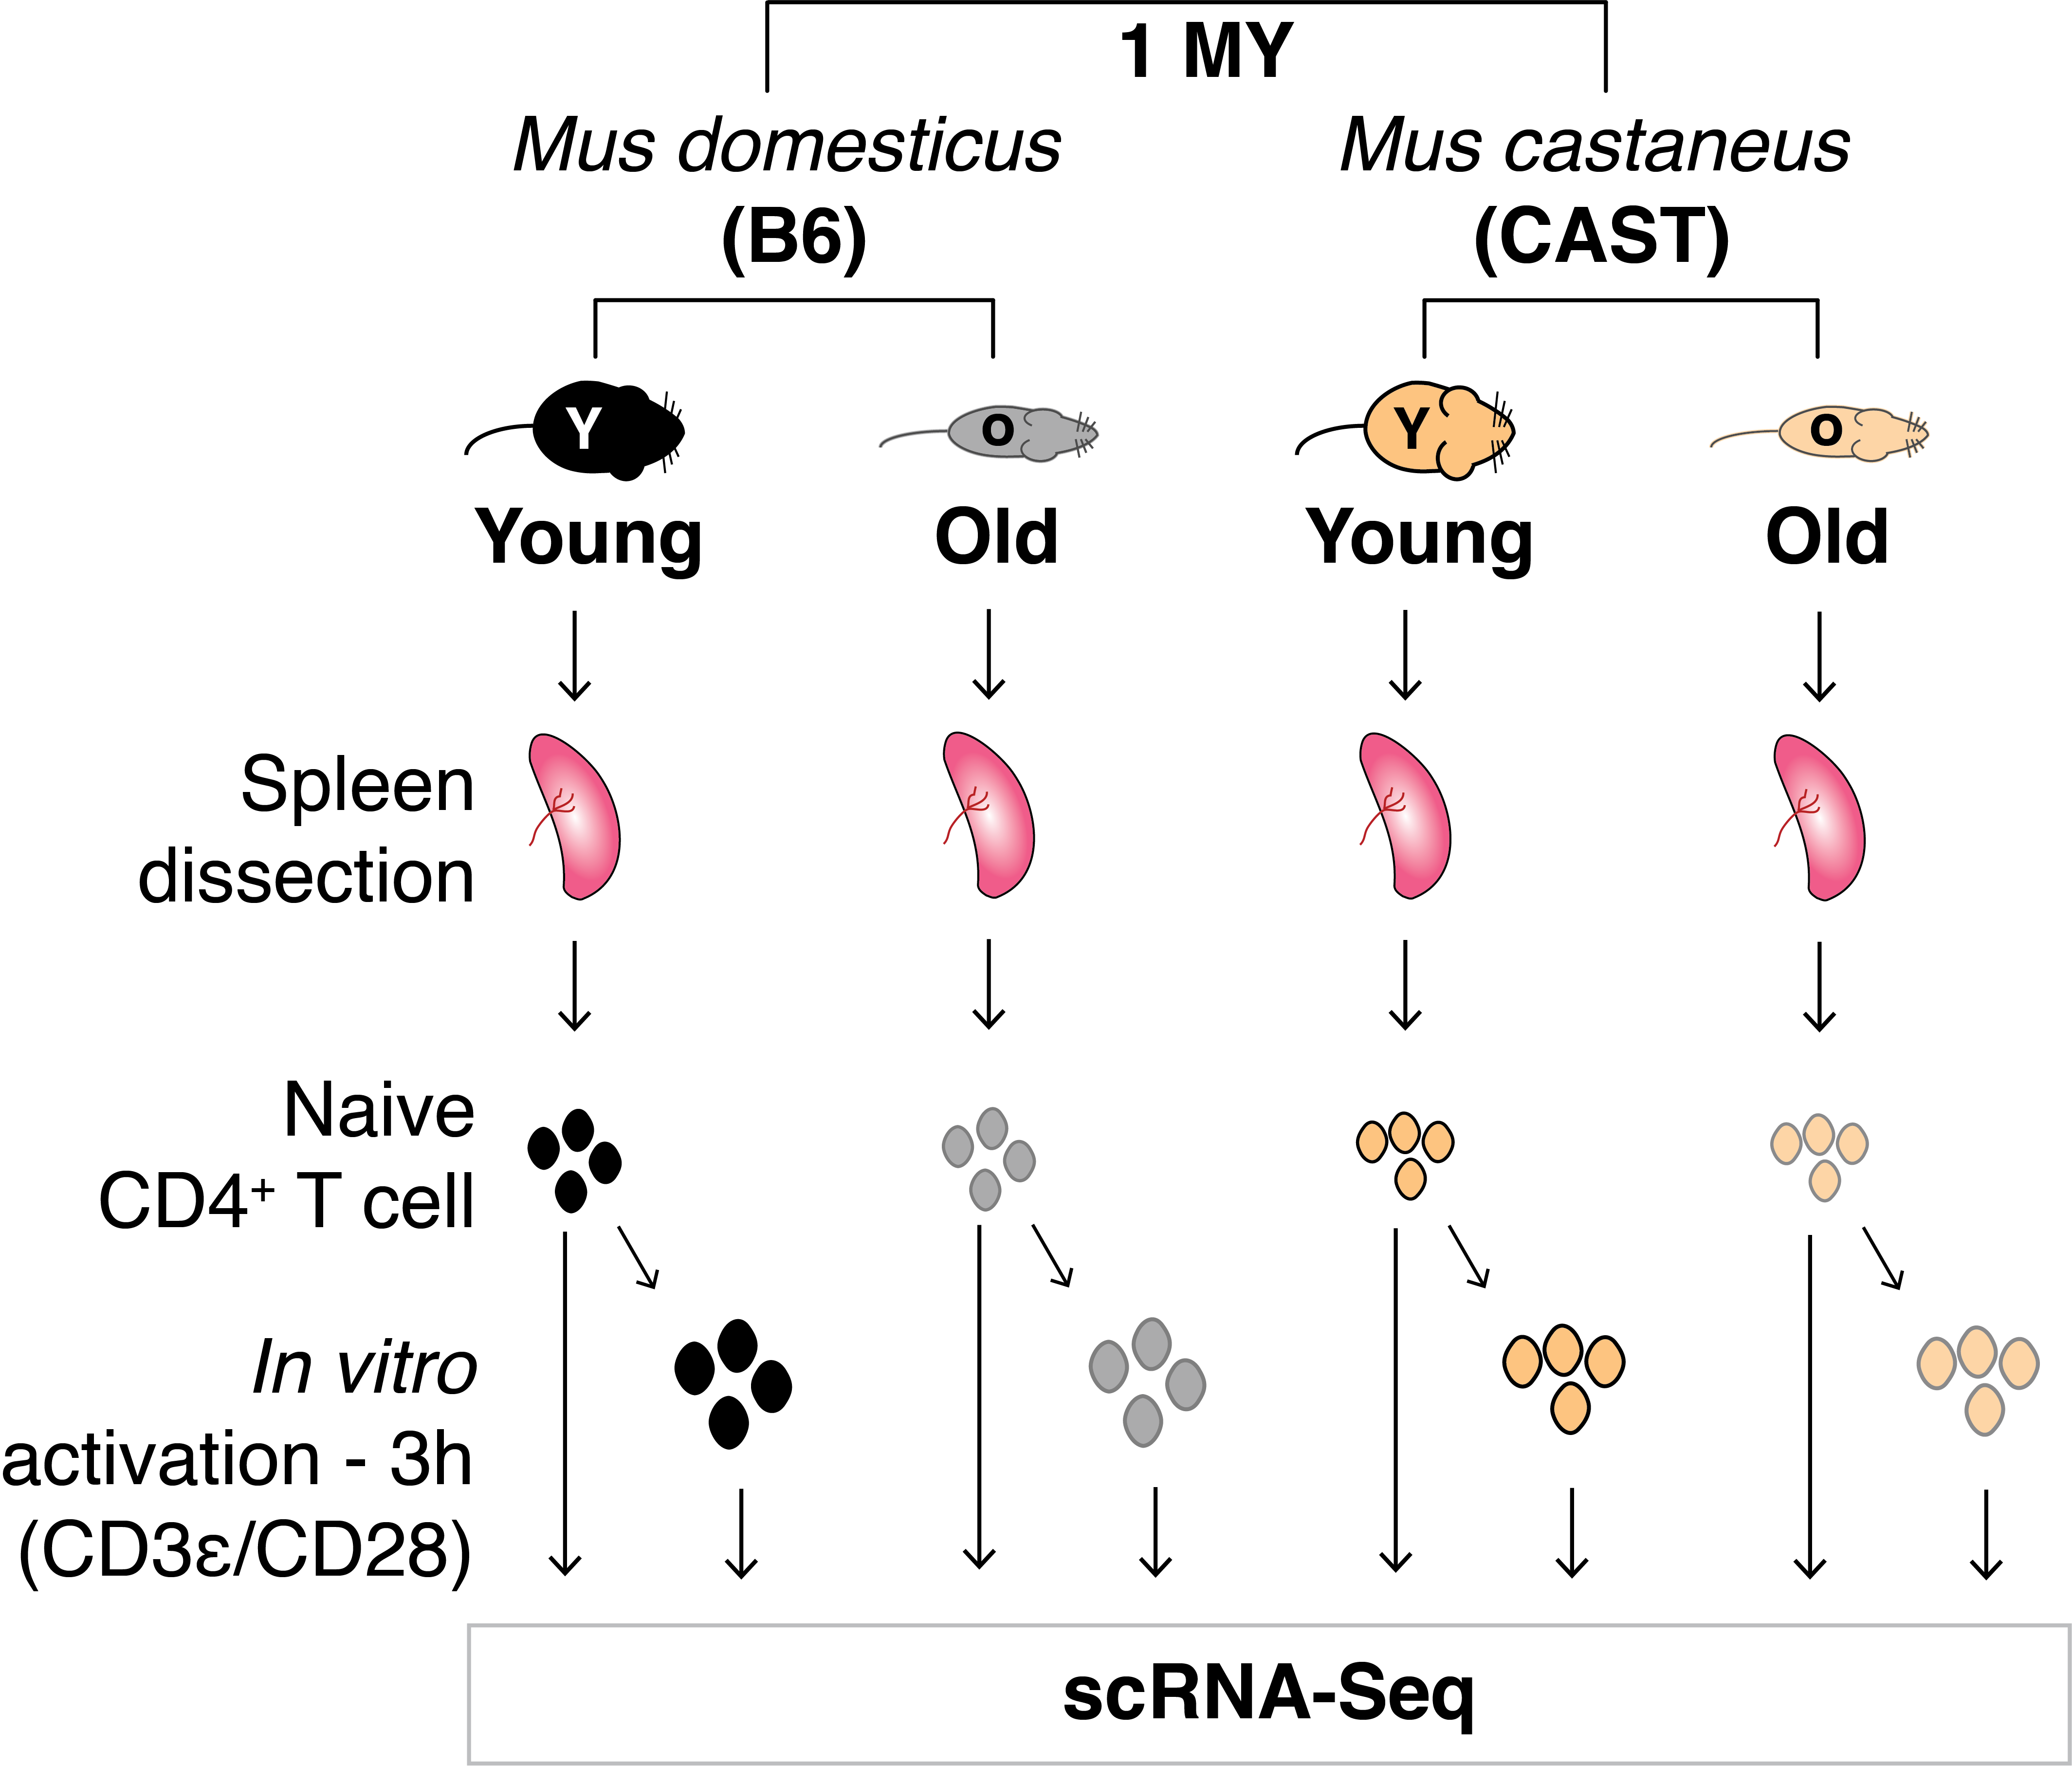
\includegraphics[width=0.48\textwidth]{Fig_1.png}
\caption[The scVI model.]{\textbf{The scVI model.} \\
Hierarchical representation of the scVI model. 
Shaded nodes indicate observed quantities. 
White nodes indicated latent random variables. 
Shaded diamonds represent constants which were set \emph{a priori}. 
White diamonds indicate variables shared across all genes and all cells. 
Edges show conditional dependency. Adapted from \citep{Lopez2018}.}
\label{fig0:scVI}
%\vspace{-60mm}
\end{wrapfigure}

In this model, the NB distribution is realised as a hierarchical formulation of $y_{n,g}$ being Poisson distributed around the latent random variable $l_n$ with an additional random effect $w_{n,g}$. Additionally, the zero-inflation of the model is controlled by the latent variable $h_{n,g}$. 
$l_n$ is a random variable that represents nuisance variation due to differences in capture efficiency and sequencing depth and correlates with log-library size. 
$l_n$ is log-normal distributed parametrised by $l_\mu,l_\sigma\in\mathbb{R}^B_+$ which are empirical mean and variance estimates of the log-library size per batch in $B$ and which are therefore constants in the model \textbf{(Fig.~\ref{fig0:scVI}A)}.\\

$w_{n,g}$ is Gamma distributed with the shape parameter $\rho_n^g$ and the scale parameter $\theta$. $\rho_g$ represents an intermediate matrix that relates the observations $x_{n,g}$ to the latent variables $z_n$. 
It provides a batch-corrected, normalised estimate of the percentage of transcripts in each cell $n$ from each gene $g$. 
$\theta$ is a global inverse-dispersion variable shared across all genes and all cells. 
The latent variable $z_n$ captures a latent representation of the data reflecting biological variation between the cells. 
$f_w$ and $f_h$ are neural networks mapping the latent space and batch annotation back to the full dimension of all genes: $\mathbb{R}^d\times{}\left\lbrace0,1\right\rbrace^B\rightarrow\mathbb{R}^G$.\\

Fast inference of this model is implemented via stochastic optimisation. First, the latent variables $w_{n,g}$, $h_{n,g}$ and $y_{n,g}$ are integrated out by controlling that $p(x_{n,g}|z_n,l_n,s_n)$ has a closed form density and is ZINB (see Appendix A in \citep{Lopez2018}). 
In this formulation, the distribution of $x_{n,g}$ is only conditioned on the latent variables $z_n$ and $l_n$. 
The posterior distributions has therefore the following form: $p(z_n,l_n|x_{n,g},s_n)$. Mean-field variational inference is used to parametrised the posterior as:

\begin{equation}
p(z_n,l_n|x_{n,g},s_n)=p(z_n|x_{n,g},s_n)p(l_n|x_{n,g},s_n)
\end{equation} 

The variational distribution $q(z_n|\cdot)$ is chosen to be Gaussian with diagonal covariance matrix and mean and covariance are learned by a \gls{MLP} network similar to Kingma \emph{et al.}, 2013 \citep{Kingma2013}. 
Similarly, $q(l_n|\cdot)$ is chosen to be log-normal where the scalar mean and variance are learned by a MLP \citep{Kingma2013}. 
The authors used reparametrisation to solve the variational lower bound of this system \cite{Lopez2018, Kingma2013}. 
Furthermore, scVI uses stochastic optimisation by sampling 128 cells for optimising the objective function. 
This approach is therefore fast (5 hours for > 1 million cells and 750 genes and 10 hours for > 1 million cells and 10,000 genes) and memory efficient. \\

The authors concluded that: 
1. scRNA-Seq data is better fitted with a ZINB than log-Normal or zero-inflated log-Normal; 2. Zero-inflation is not needed as part of the model since the zeros in dataset can be explained by NB distribution; 
3. When the number of cells is smaller than number of genes, scVI underfits the data \citep{Lopez2018}. 
The clear strength of the model is the fast estimation of model parameters that can be used for down-stream analysis (e.g. visualisation, normalisation, differential expression testing). 
The draw-back of this model is the inability to obtain gene-specific variability estimates but rather global variability measures calculated on the latent space. \\

As a future direction, generative models need to allow fast inference while providing interpretable model parameters that capture gene-specific measures of transcriptional noise. 
These measures should ideally be independent of technical noise, mean expression and possibly flexible enough to adjust for further confounding factors such as expression changes over a differentiation time course. 
 




% *************************************
% **** Back Matter 
% *************************************

% Backmatter should be commented out, if you are using appendices after References
%\backmatter

% *************************************
% **** Bibliography 
% *************************************

\begin{spacing}{0.9}

% To use the conventional natbib style referencing
% Bibliography style previews: http://nodonn.tipido.net/bibstyle.php
% Reference styles: http://sites.stat.psu.edu/~surajit/present/bib.htm

%\bibliographystyle{apalike}
\bibliographystyle{unsrt} % Use for unsorted references  
%\bibliographystyle{plainnat} % use this to have URLs listed in References
\cleardoublepage
%\bibliography{References/library} % Path to your References.bib file


% If you would like to use BibLaTeX for your references, pass `custombib' as an option in the document class. The location of 'reference.bib' should be specified in the preamble.tex file in the custombib section. Comment out the lines related to natbib above and uncomment the following line.

%\printbibliography[heading=bibintoc, title={References}]


\end{spacing}

% *************************************
% **** Appendices 
% *************************************

\begin{appendices} % Using appendices environment for more functunality

%!TEX root = ../main.tex
% ******************************************
% 			Thesis Appendix A 
% ******************************************

\chapter{Experimental methods} 

\section{Ageing increases transcriptional noise \\
in CD4\plus{} T cell activation}
\markboth{Experimental methods}{A.1 Ageing increases transcriptional noise in CD4\plus{} T cell activation}
\label{appA.1}

\subsection{Mouse material}

CAST/EiJ male mice were maintained under specific pathogen-free conditions at the University of Cambridge, CRUK – Cambridge Institute under the auspices of a UK Home Office license. 
Inbred wild-type C57BL/6 mice were purchased from Charles River UK Ltd (Margate, United Kingdom). 
Animals were euthanized in accordance with Schedule 1 of the Animals (Scientific Procedures) Act 1986. 
Each animal used was macroscopically examined. 
Animals with lesions or phenotypic alterations in their internal organs were discarded. 

\subsection{CD4\plus{} T cell isolation}
\label{appA.1:isolation}

Unstimulated CD4\plus{} T cells were purified from dissociated mouse spleens using EASY cell strainer (30 \textmu{}m, Greiner BioOne), cell separation media (lympholyte, \#{}CL5035) and the CD4\plus{} CD62L\plus{} T Cell Isolation Kit II (Miltenyi Biotec, \#{}130-093-227). 
Flow cytometry confirmed that 96.4\% of the isolated CD4\plus{} T cells were naive in young B6 \textbf{(Fig.~\ref{fig1:characterization}D)}. 
Naive CD4\plus{} T cells formed a single, high-purity population in young animals. Old animals had a small population of CD4\plus{} T cells with slightly elevated CD44 levels, reduced CD62L expression, and attenuated activation dynamics \textbf{(Fig.~\ref{fig1:characterization}E-G)}; 
their removal did not impact the results presented in \textbf{Chapter 2} \textbf{(Fig.~\ref{fig1:validation}D)}.\\

Purified unstimulated CD4\plus{} T cells were cultured in IMDM medium (GIBCO, \#{}21980-032) supplemented with 10\% Fetal Bovine Serum (Life Technology, \#{}10500064), 1 \textmu{}g/mL Penicillin/Streptomicin (Life Technology, \#{}15070063), and 50 \textmu{}M 2-mercaptoethanol (Gibco, \#{}31350-010). 
Cells were seeded into 96-well plates coated for 1h at 37$^\circ$C with anti-CD3\textepsilon{} (1 \textmu{}g/ml, clone: 145-2C11, eBioscience, \#{}16-0031-82) and anti-CD28 (3 \textmu{}g/ml, clone: 37.51, eBioscience, \#{}16-0281-82) at a density of 80,000-120,000 cells/ml, and then cultured in a total volume of 100 \textmu{}l media that did not contain cytokines or additional antibodies.  \\

All cells were cultured in a humidified incubator at 37$^\circ$C, with 5\% CO2. Unstimulated and activated CD4\plus{} T cells were then immediately collected and loaded on a 5–10\textmu{}m Auto Prep Integrated Fluidic Circuit (IFC; Fluidigm, San Francisco, CA) to capture single cells using the C1 single-cell Auto Prep System (Fluidigm). 
All IFCs were visually inspected, and wells with multiple cells or cell debris were identified per instructions of the manufacturer (PN 101-2711 A1 White Paper). 
Upon cell capture, reverse transcription and cDNA amplification were performed using the SMARTer PCR cDNA Synthesis Kit (Clontech) and the Advantage 2 PCR Kit (Clontech). 
ERCC spike-in RNA (Ambion) (1 \textmu{}L diluted at 1:50,000) was added to the C1 lysis mix. 
All the capture sites were included for the RNA-seq library preparation, and wells identified above as multiple cells or containing debris were removed during computational analysis.

\subsection{Flow cytometry}
\label{appA.1:FACS}

Unstimulated CD4\plus{} T cells were purified from spleens of young and old C57BL/6 mice (see above). 
Isolated cells were, directly or after 3h activation in vitro (see above), incubated with TruStainfcX (anti-mouse CD16/32, clone:93, BioLegend) before staining with immunofluorescence conjugated antibodies against murine CD4 (clone: RM4-5, BioLegend), CD44 (clone: IM7, BioLegend), CD62L (clone: MEL-14, BioLegend), CD25 (clone: 3C7, BioLegend), CD69 (clone: H1.2F3, BioLegend), CD127 (clone: A7R34, BioLegend), and KLRG1 (clone: 2F1, BD Biosciences). 
Cell viability was determined using Fixable eFluor 780 viability dye (eBioscience). 
Data were acquired on a 5-laser Aria IIu SORP instrument (BD Biosciences) and data analysis was performed using FlowJo software (Tree Star).\\

Naive and effector memory CD4\plus{} T cells were purified from spleens of both young and old C57BL/6 mice by FACS.  
Briefly, spleens were harvested from both young and old animals and single cell suspensions were obtained by meshing through a cell strainer (70 \textmu{}m). 
B cells were depleted from cell suspensions by MACS using CD19 microbeads (Miltenyi Biotec, \#{}130-052-201) and red blood cells were lysed with RBC lysis buffer (Biolegend, \#{}B205551). 
The enriched cell fraction was then stained with Fixable eFluor 780 viability dye (eBioscience) following by Fc receptor blocking with TruStain fcXTM (clone: 39, Biolegend) and subsequent staining with a panel of fluorescence-conjugated antibodies against CD4 (clone: RM4-5, BioLegend), CD44 (clone: IM7, BioLegend), CD62L (clone: MEL-14, BioLegend), CD24 (clone: M1/69, BioLegend), Qa2 (clone: 695H1-9-9, BioLegend), CD69 (clone: H1.2F3, BioLegend) and PD-1 (clone: RMP1-30, BioLegend).  
Stained cells were immediately sorted using a 5-laser Aria IIu SORP instrument (BD Biosciences) with the stringent gating strategy described in \textbf{Fig.~\ref{fig1:FACS}}. 

\subsection{ScRNA-Seq library preparation and sequencing}
\label{appA.1:RNA-Seq}

ScRNA-Seq libraries were prepared using standard Fluidigm protocol (\# PN 100-7168 K1) based on SMARTer chemistry and Illumina Nextera XT (Illumina) using paired-end 125bp sequencing on Illumina HiSeq2500. 
Each RNA-seq library was sequenced to a typical depth of 1.3 million reads on average. 
To account for potential batch effects, for each experimental condition, two biological replicates were prepared using independent C1 IFCs.

\newpage

\section{Transcriptional dynamics during spermatogenesis \\ at single-cell resolution}
\markboth{Experimental methods}{A.2 Transcriptional dynamics during spermatogenesis at single-cell resolution}
\label{appA.2}

\subsection{Mouse material}

All animals were housed in the Biological Resources Unit (BRU) in the Cancer Research UK – Cambridge Institute under Home Office Licences PPL 70/7535 until February 2018 and PPL P9855D13B from March 2018. 
C57BL/6 animals were purchased from Charles River UK Ltd (Margate, United Kingdom).
 
\subsection{FACS of spermatogenic cell populations}
\label{appA.2.sorting}

Spermatogenic cell populations were isolated from adult mouse testes as described in Ernst \emph{et al.}, 2016 \citep{Ernst2016}. 
In brief, the albuginea was removed and tissue was incubated in dissociation buffer containing 25 mg/ml Collagenase A, 25 mg/ml Dispase II and 2.5 mg/ml DNase I for 30 minutes at 37$^\circ$C. Enzymatic digestion was quenched with Dulbecco’s Modified Eagle Medium (DMEM, Gibco) supplemented with 10\% Fetal calf serum (FCS, 10270106, Gibco). 
Cells were resuspended at a concentration of 1 million cells per ml and stained with Hoechst 33342 (H3570, ThermoFisher Scientific) at a final concentration of 5 µg/ml for 45 minutes at 37$^\circ$C. 
Cells were resuspended in PBS containing 1\% FCS and 2 mM EDTA and propidium iodide was added to a final concentration of 1 µg/ml prior to sorting. \\
Cells were sorted on an Aria IIu cell sorter (Becton Dickinson) using a 100 \textmu{}m nozzle. 
Hoechst was excited with a UV laser at 355nm and fluorescence was recorded with a 450/50 filter (Hoechst blue) and 635LP filter (Hoechst red). 
Primary spermatocytes (4N) and round spermatids (1N) were sorted and collected in PBS containing 1\% FCS and 2 mM EDTA. 

\subsection{Total RNA-Seq from bulk samples}
\label{appA.2.bulk}

Testes from prepubertal mice ranging between postnatal day 6 and 35 were flash frozen or directly used for RNA extraction using Trizol (Thermo Fisher, 15596026) following manufacturer’s instructions. 
Purified RNA was DNase-treated using the TURBO DNA-free Kit according to manufacturer’s instructions (Thermo Fisher, AM1907) and RNA quality was assessed using the Agilent Tapestation RNA Screentape. 
800 ng of DNA-depleted RNA were used for RNA-Seq library preparation using the TruSeq Stranded Total RNA Library Kit with Ribo-Zero Gold for cytoplasmic and mitochondrial ribosomal RNA removal according to manufacturer’s instructions (Illumina, RS-122-2303). 
Libraries were then sequenced on Illumina HiSeq2500 using a paired-end 125bp run. 

\subsection{10X Genomics single-cell RNA-Seq}

Mouse testes were enzymatically dissociated as described above and 34 µl of single-cell suspension at a concentration of ~297,000 cells/ml was loaded into one channel of the ChromiumTM Single Cell A Chip (10X Genomics\textsuperscript{\textregistered}), aiming for a recovery of 4000-5000 cells. 
The Chromium Single Cell 3’ Library \& Gel Bead Kit v2 (10X Genomics\textsuperscript{\textregistered}, 120237) was used for single-cell barcoding, cDNA synthesis and library preparation, following manufacturer’s instructions according to the Single Cell 3’ Reagent Kits User Guide Version 2, Revision D. 
Libraries were sequenced on Illumina HiSeq2500 using a paired-end run sequencing 26bp on read 1 and 98bp on read 2. 

\subsection{Histology}
Testes were fixed in neutral buffered formalin (NBF) for 24 hours, transferred to 70\% ethanol, machine processed and paraffin embedded. 
Formalin-fixed paraffin-embedded (FFPE) sections of 3\textmu{}m thickness were used for all histological stains and immunohistochemistry (IHC). 
For Periodic Acid Schiff (PAS) stainings slides were dewaxed, washed in water and placed in 0.5\% Periodic Acid (Sigma P0430) for 5 minutes. After three washes in ultra-pure water, slides were placed in Schiff reagent (Thermo Fisher Scientific, J/7300/PB08) for 15-30 minutes in a closed container and washed again three times in ultra-pure water. 
Counterstain was performed using Mayers Haematoxylin (Thermo Fisher Scientific, LAMB/170-D) for 40 seconds followed by rinsing in tap water, dehydration and mounting. IHC was performed on FFPE sections using the Bond\textsuperscript{TM} Polymer Refine Kit (DS9800, Leica Microsystems) on the automated Bond Platform. Anti-phospho-Histone H3 (Ser10) (pH3) antibody (Upstate, 06-570, 1:200 dilution) was used with DAB Enhancer (Leica Microsystems, AR9432) and heat-induced epitope retrieval was performed for 10 minutes at 100$^\circ$C on the Bond platform with sodium citrate. 
All slides were scanned using Aperio XT (Leica Biosystems) and PH3 intensities were quantified using the Aperio eSlide Manager (Leica Biosystems). 

\newpage

\subsection{Low cell number chromatin profiling using CUT\&{}RUN}
\label{appA.2.CnR}

\emph{In situ} chromatin profiling of FACS-purified spermatogenic cell populations was performed according to Skene \emph{et al.}, 2018 \citep{Skene2018}. 
In brief, spermatocytes and spermatids were sorted as described above and collected in PBS. Cells were spun down at 600g for 3 minutes in swinging-bucket rotor and washed twice with 1.5 ml Wash buffer (20 mM HEPES-KOH (pH 7.5), 150 mM NaCl, 0.5 mM Spermidine and 1X cOmplete\texttrademark{} EDTA-free protease inhibitor cocktail (04693159001, Roche)). 
During the cell washes, concanavalin A-coated magnetic beads (Bangs Laboratories, cat. No BP531) (10 \textmu{}l per condition) were washed twice in 1.5 mL Binding Buffer (20 mM HEPES-KOH (pH 7.5), 10 mM KCl, 1mM CaCl, 1mM MnCl2) and resuspended in 10 \textmu{}l Binding Buffer per condition. 
Cells were then mixed with beads and rotated for 10 minutes at room temperature (RT) and samples were split into aliquots according to number of antibodies profiled per cell type. We used 20,000-30,000 spermatocytes and 40,000-60,000 spermatids per chromatin mark.\\ 

Cells were then collected on magnetic beads and re-suspended in 50 \textmu{}l Antibody Buffer (Wash buffer with 0.05\% Digitonin and 2 mM EDTA) containing one of the following antibodies in 1:100 dilution: 
H3K4me3 (Millipore 05-1339 CMA304, Lot2780484) and H3K9me3 (Abcam, ab8898, Lot GR306402-1). 
Cells were incubated with antibodies for 10 minutes at RT and then washed once with 1 ml Digitonin buffer (Wash buffer with 0.05\% Digitonin). 
For the mouse anti-H3K4me3 antibody, samples were incubated with a 1:100 dilution in Digitonin buffer of secondary rabbit anti-mouse antibody (Invitrogen, A27033, Lot RG240909) for 10 minutes at RT and then washed once with 1 mL Digitonin buffer. 
Samples were then incubated with 700 ng/ml ProteinA-MNase fusion protein (kindly provided by Steven Henikoff) for 10 minutes at room temperature followed by two washes with 1 ml Digitonin buffer. 
Cells were then resuspended in 100 µl Digitonin buffer and cooled down to 4$^\circ$C before addition of CaCl$_2$ to a final concentration of 2 mM. 
Targeted digestion was performed for 30 minutes on ice until 100 µl of 2X STOP buffer (340 mM NaCl, 20 mM EDTA, 4 mM EGTA, 0.02\% Digitonin, 250 mg RNase A, 250 \textmu{}g Glycogen, 15 pg/ml yeast spike-in DNA (kindly provided by Steven Henikoff)) were added. 
Cells were then incubated at 37$^\circ$C for 10 minutes to release cleaved chromatin fragments, spun down for 5 minutes at 16,000 g at 4$^\circ$C and collected on magnet. 
Supernatant containing the cleaved chromatin fragments was then transferred and cleaned up using the Zymo Clean \& Concentrator Kit.
Library preparation was performed using the ThruPLEX\textsuperscript{\textregistered} DNA-Seq Library Preparation Kit (R400407, Rubicon Genomics) with a modified Library Amplification programme: 
Extension and cleavage for 3 minutes at 72$^\circ$C followed by 2 minutes at 85$^\circ$C, denaturation for 2 minutes at 98$^\circ$C followed by four cycles of 20 seconds at 98$^\circ$C, 20 seconds at 67$^\circ$C and 40 seconds at 72$^\circ$C for the addition of indexes. 
Amplification was then performed for 12-14 cycles of 20 seconds at 98$^\circ$C and 15 seconds at 72$^\circ$C. 
Average library size was tested on Agilent 4200 Tapestation using a DNA1000 High Sensitivity Screentape and quantification was performed using the KAPA Library Quantification Kit (Kapa Biosystems). 
CUT\&{}RUN libraries were sequenced on a HiSeq2500 using a paired-end 125bp run. 


%!TEX root = ../thesis.tex
% ******************************************
% 			Thesis Appendix B
% ******************************************

\chapter{Computational methods} 

\section{Addressing the mean confounding effect for differential variability testing}
\label{appB.1}

\subsection{Prior specifications of extended BASiCS model}

\begin{align*}
\mu_i &\ind \mbox{log-Normal}\left(0, s^2_{\mu}\right) \\
\delta_i| \mu_i,\beta,\sigma^2, \lambda_i, \eta &\ind \text{log-N}\left( \text{f}(\mu_i),\frac{\sigma^2}{\lambda_i} \right)\\
\lambda_i|\eta &\ind \text{Gamma}\left(\frac{\eta}{2},\frac{\eta}{2}\right)\\
\beta|\sigma^2 & \sim \textnormal{Normal}(m_\beta,\sigma^2V_\beta),\\
\sigma^2 & \sim  \textnormal{Inv-Gamma}(a_{\sigma^2},b_{\sigma^2}),\\
s_j & \iid  \textnormal{Gamma}(a_s,b_s) \\
(\phi_1, \ldots, \phi_n)' & \sim  n \times \textnormal{Dirichlet}(a_\phi),\\
\theta & \sim  \textnormal{Gamma}(a_\theta,b_\theta)
\end{align*}

\subsection{Starting values for hyper-parameter}
\label{appB.1.hyper}

\todo{list hyper-parameter values}
\begin{align*}
m_{\beta} & = \mathbf{0}_L \hspace{0.2cm} \text{(an $L$-dimensional vector of zeroes)}\\
V_{\beta} & = \mathbf{I}_L \hspace{0.2cm} \text{(an $L$-dimensional identity matrix)}\\
a_{\sigma^2} & = 2\\
b_{\sigma^2} & = 2\\
s^2_{\mu}& =  \\
m_\beta& =  \\
V_\beta& =  \\
a_{\sigma^2}& =  \\
b_{\sigma^2}& =  \\
a_s& =  \\
b_s& =  \\
a_\phi& =  \\
a_\theta& =  \\
b_\theta& = 
\end{align*}

\subsection{Likelihood of extended BASiCS model}

The likelihood function of the extended BASiCS model takes the form:

\begin{align} \label{eq::loglik}
\Lagr = & \left[\prod_{i=1}^{q_0}\prod_{j=1}^n\frac{\Gamma(x_{ij}+\frac{1}{\delta_i})}{\Gamma(\frac{1}{\delta_i})x_{ij}!}\left(\frac{\frac{1}{\delta_i}}{\phi_j\nu_j\mu_i+\frac{1}{\delta_i}}\right)^\frac{1}{\delta_i}\left(\frac{\phi_j\nu_j\mu_i}{\phi_j\nu_j\mu_i+\frac{1}{\delta_i}}\right)^{x_{ij}}\right] \nonumber\\ 
&\times\left[\prod_{i=q_0+1}^{q}\prod_{j=1}^n\frac{(\nu_j\mu_i)^{x_{ij}}}{x_{ij}!}\exp\lbrace-\nu_j\mu_i\rbrace\right]\times{}\left[\prod_{j=1}^n\frac{(s_j\theta)^{-\frac{1}{\theta}}}{\Gamma(\frac{1}{\theta})}\nu_j^{\frac{1}{\theta}-1}\exp\left\lbrace-\frac{\nu_j}{s_j\theta}\right\rbrace\right].
\end{align} 

\subsection{Derivation of full conditionals for extended BASiCS model}

To calculate the full conditionals ($\pi^*(\cdot)$) for Gibbs sampling, the likelihood ($\Lagr_j$ for cell-specific likelihood, $\Lagr_i$ for gene-specific likelihood) is multiplied by the relevant prior specifications ($\pi(\cdot)$). $q_0$ indicates the number of biological genes while $q$ is the number of biological and spike-in genes. $L$ is the number of Gaussian Radial Basis Functions. $\Lambda$ is a diagonal matrix with elements $(\lambda_1, \ldots, \lambda_{q_0})$ and $Y = (\log(\delta_1), \ldots, \log(\delta_{q_0}))'$.\\ 

Full conditional for $\mu_i$ across all cells:
\begin{fleqn}
\begin{align*}
&\pi^*(\mu_i|\cdot)&&\propto{} \Lagr_i\times\pi(\mu_i)\times\pi(\delta_i|\mu_i,\beta,\sigma^2,\eta)\\
& &&\propto{}\left[\prod_{j=1}^n\left(\frac{1}{\phi_j\nu_j\mu_i+\frac{1}{\delta_i}}\right)^\frac{1}{\delta_i}\left(\frac{\mu_i}{\phi_j\nu_j\mu_i+\frac{1}{\delta_i}}\right)^{x_{ij}}\right]\times\exp\left(-\frac{(\log(\mu_i)-0)^2}{2a_\mu^2}\right)\frac{1}{\mu_i}\\
& &&\times\exp\left\lbrace-\frac{\lambda_i}{2\sigma^2}(\log(\delta_i)-f(\mu_i))^2\right\rbrace\\
& &&\propto\left[\prod_{j=1}^n{}\frac{(\mu_i)^{x_{ij}}}{(\phi_j\nu_j\mu_i+\frac{1}{\delta_i})^{\frac{1}{\delta_i}+x_{ij}}}\right]\times{}\exp\left(-\frac{(\log(\mu_i))^2}{2a_\mu^2}-\frac{\lambda_i(\log(\delta_i)-f(\mu_i))^2}{2\sigma^2}\right)\frac{1}{\mu_i}\\
& &&\propto{}\frac{\mu_i^{\sum_{j=1}^n{}x_{ij}}}{\prod_{j=1}^n{}(\phi_j\nu_j\mu_i+\frac{1}{\delta_i})^{\frac{1}{\delta_i}+x_{ij}}}\times{}\exp\left(-\frac{(\log(\mu_i))^2}{2a_\mu^2}-\frac{\lambda_i(\log(\delta_i)-f(\mu_i))^2}{2\sigma^2}\right)\frac{1}{\mu_i}
\end{align*}
\end{fleqn}

Full conditional for $\delta_i$ across all cells:
\begin{fleqn}
\begin{align*}
&\pi^*(\delta_i|\cdot)&&\propto{} \Lagr_i\times\pi(\delta_i|\mu_i,\beta,\sigma^2,\eta)\\
& &&\propto{}\left[\prod_{j=1}^n\frac{\Gamma(x_{ij}+\frac{1}{\delta_i})}{\Gamma(\frac{1}{\delta_i})}\left(\frac{\frac{1}{\delta_i}}{\phi_j\nu_j\mu_i+\frac{1}{\delta_i}}\right)^\frac{1}{\delta_i}\left(\frac{1}{\phi_j\nu_j\mu_i+\frac{1}{\delta_i}}\right)^{x_{ij}}\right]\\
& &&\times\exp\left\lbrace-\frac{\lambda_i(\log(\delta_i)-f(\mu_i))^2}{2\sigma^2}\right\rbrace\frac{1}{\delta_i}\\
& &&\propto\left[\prod_{j=1}^n\frac{\Gamma(x_{ij}+\frac{1}{\delta_i})}{\Gamma(\frac{1}{\delta_i})}\frac{(\frac{1}{\delta_i})^{\frac{1}{\delta_i}}}{(\phi_j\nu_j\mu_i+\frac{1}{\delta_i})^{\frac{1}{\delta_i}+x_{ij}}}\right]\times{}\exp\left\lbrace-\frac{\lambda_i(\log(\delta_i)-f(\mu_i))^2}{2\sigma^2}\right\rbrace\frac{1}{\delta_i}\\
\end{align*}
\end{fleqn}

Full conditional for $\beta$ across all cells and genes:
\begin{fleqn}
\begin{align*}
\pi^*(\beta|\cdot)&\propto{} \Lagr\times\pi(\delta|\mu,\beta,\sigma^2,\eta)\times\pi(\beta)\\
&\propto{}\exp\lbrace-\frac{1}{2\sigma^2}[(Y-X\beta)'\Lambda(Y-X\beta)\rbrace\times\\
&(\frac{1}{\sigma^2})^{\frac{k}{2}}\exp\lbrace-\frac{1}{2\sigma^2}(\beta-m_\beta)'V_\beta^{-1}(\beta-m_\beta)\rbrace\\
&\propto{}\exp\lbrace-\frac{1}{2\sigma^2}[(Y-X\beta)'\Lambda(Y-X\beta)+(\beta-m_\beta)'V_\beta^{-1}(\beta-m_\beta)]\rbrace\\
&\propto{}\exp\lbrace-\frac{1}{2\sigma^2}[Y'\Lambda{}Y-2(X\beta)'\Lambda{}Y+(X\beta)'\Lambda{}X\beta\\
&+\beta'V_\beta^{-1}\beta-2m_\beta'V_\beta^{-1}\beta+m_\beta{}V_\beta^{-1}m_\beta{}]\rbrace\\
&\propto{}\exp\lbrace-\frac{1}{2\sigma^2}[\beta'X'\Lambda{}X\beta+\beta'V_\beta^{-1}\beta-2X'\Lambda{}Y\beta-2V_\beta^{-1}m_\beta\beta]\rbrace\\
&\propto{}\exp\lbrace-\frac{1}{2\sigma^2}[\beta'(X'\Lambda{}X+V_\beta^{-1})\beta-2(X'\Lambda{}Y+V_\beta^{-1}m_\beta)\beta]\rbrace\\
&\propto{}N(m^*_\beta,\sigma^2V^*_\beta)
\end{align*}
\end{fleqn} With
\begin{fleqn}
\begin{align*}
V^*_\beta&=(X'\Lambda{}X+V_\beta^{-1})^{-1}\\
m^*_\beta&=(X'\Lambda{}X+V_\beta^{-1})^{-1}(X'\Lambda{}Y+V_\beta^{-1}m_\beta{})
\end{align*}

Full conditional for $\lambda_i$ across all cells:
\begin{fleqn}
\begin{align*}
\pi^*(\lambda_i|\cdot)&\propto{}\Lagr_i\times\pi(\delta_i|\mu,\beta,\sigma^2,\eta)\times\pi(\lambda_i)\\
&\propto{}\lambda_i^{1/2}\exp\lbrace-\frac{\lambda_i}{2\sigma^2}(\log(\delta_i)-f(\mu_i))^2\rbrace\cdot\lambda_i{}^{\frac{\eta}{2}-1}\exp(-\lambda_i{}\frac{\eta}{2})\\
&\propto{}\lambda_i^{\frac{\eta+1}{2}-1}\exp\lbrace-\frac{\lambda_i}{2}(\eta+\frac{1}{\sigma^2}(\log(\delta_i)_i-f(\mu_i)))\rbrace\\
&\propto{}\textnormal{Gamma}(a^*_\lambda,b^*_\lambda)
\end{align*}
\end{fleqn}
With
\begin{align*}
a^*_\lambda&=\frac{\eta+1}{2}\\
b^*_\lambda&=\frac{1}{2}\left[\frac{1}{\sigma^2}(\log(\delta_i)-f(\mu_i))^2+\eta\right]
\end{align*}
\end{fleqn}

Full conditional for $\sigma^2$ across all cells and genes:
\begin{fleqn}
\begin{align*}
\pi^*(\sigma^2|\cdot)&\propto{}\Lagr\times\pi(\delta|\mu,\beta,\sigma^2,\eta)\times\pi(\sigma^2)\\
&\propto{}\left(\frac{1}{\sigma^2}\right)^{\frac{q_0}{2}}\exp\lbrace-\frac{1}{2\sigma^2}(Y-X\beta)'\Lambda(Y-X\beta)\rbrace\\
&\cdot\left(\frac{1}{\sigma^2}\right)^{L+2}\exp\lbrace-\frac{1}{2\sigma^2}(\beta-m_\beta{})'V_\beta^{-1}(\beta-m_\beta{})\rbrace\\
&\cdot\left(\frac{1}{\sigma^2}\right)^{a_{\sigma^2}+1}\exp\lbrace-\frac{b_{\sigma^2}}{\sigma^2}\rbrace\\
&\propto{}\left(\frac{1}{\sigma^2}\right)^{\frac{q_0+L+2}{2}+a_{\sigma^2}+1}\exp\lbrace-\frac{1}{\sigma^2}[b_{\sigma^2}+\frac{1}{2}[(Y-X\beta)'\Lambda(Y-X\beta) \\
&+ (\beta-m_\beta{})'V_\beta^{-1}(\beta-m_\beta{})]]\rbrace
\end{align*}
\end{fleqn} 
After completing the squares
\begin{fleqn}
\begin{align*}
&\propto{}\left(\frac{1}{\sigma^2}\right)^{\frac{q_0+L+2}{2}+a_{\sigma^2}+1}\exp\lbrace-\frac{1}{\sigma^2}[b_{\sigma^2}+\frac{1}{2}(Y'\Lambda{}Y+m_\beta{}'V_\beta{}^{-1}m_\beta{}\\
&+(\beta-m^*_{\beta})'(V^*_{\beta})^{-1}(\beta-m^*_{\beta})-(m^*_{\beta})'(V^*_{\beta})^{-1}m^*_{\beta})]\rbrace\\
&\propto{}(\frac{1}{\sigma^2})^{a_{n,\sigma^2}+1}\exp(-\frac{b^*_{\sigma^2}}{\sigma^2})\\
&\propto{}\textnormal{Inv-Gamma}(a^*_{\sigma^2},b^*_{\sigma^2})
\end{align*}
\end{fleqn}
With
\begin{fleqn}
\begin{align*}
a^*_{\sigma^2}&=\frac{q_0+L+2}{2}+a_{\sigma^2}\\
b^*_{\sigma^2}&=b_{\sigma^2}+\frac{1}{2}(Y'\Lambda{}Y+m_\beta'V_\beta^{-1}m_\beta+(\beta-m^*_{\beta})'(V^*_{\beta})^{-1}(\beta-m^*_{\beta})-(m^*_{\beta})'(V^*_{\beta})^{-1}m^*_{\beta})\\
&\equiv{}b_{\sigma^2}+\frac{1}{2}(Y'\Lambda Y+ m'_{\beta} V_\beta^{-1} m_\beta + \beta' (V^*_{\beta})^{-1} \beta - 2 \beta' (V^*_{\beta})^{-1} m^*_{\beta} )
\end{align*}
\end{fleqn}

Full conditional for $s_j$ across all genes:
\begin{fleqn}
\begin{align*}
\pi^*(s_j|\cdot)&\propto{}\Lagr_j\times\pi(s_j)\\
&\propto{}s_j{}^{a_s-1}\exp\lbrace-b_ss_j\rbrace{}s_j{}^{-\frac{1}{\theta}}\exp\lbrace-\frac{\nu_j}{s_j\theta}\rbrace\\
&\propto{}s_j{}^{a_s-\frac{1}{\theta}-1}\exp\lbrace-\frac{\nu_j}{s_j\theta}-b_ss_j\rbrace
\end{align*}
\end{fleqn}

Full conditional for $\phi$ across all genes and cells:
\begin{fleqn}
\begin{align*}
\pi^*(\phi_j|\cdot)&\propto{}\Lagr_j\times\pi(\phi_j)\\
&\propto{}\prod_{i=1}^{q_0}\prod_{j=1}^{n}\left(\frac{1}{\phi_j\nu_j\mu_i+\frac{1}{\delta_i}}\right)^\frac{1}{\delta_i}\left(\frac{\phi_j}{\phi_j\nu_j\mu_i+\frac{1}{\delta_i}}\right)^{x_{ij}}\times{}\pi(\phi_j)\\
&\propto{}\frac{\prod_{i=1}^{q_0}\prod_{j=1}^{n}\phi_j{}^{x_{ij}}}{\prod_{i=1}^{q_0}\prod_{j=1}^{n}(\phi_j\nu_j\mu_i+\frac{1}{\delta_i})^{\frac{1}{\delta_i}+x_{ij}}}\times{}\pi(\phi_j)\\
&\propto{}\frac{\prod_{i=1}^{q_0}\phi_j{}^{\sum_{j=1}^nx_{ij}}}{\prod_{i=1}^{q_0}\prod_{j=1}^{n}(\phi_j\nu_j\mu_i+\frac{1}{\delta_i})^{\frac{1}{\delta_i}+x_{ij}}}\times{}\pi(\phi_j)
\end{align*}
\end{fleqn}

Full conditional for $\nu_j$ across all genes:
\begin{fleqn}
\begin{align*}
\pi^*(\nu_j|\cdot)&\propto{}\Lagr_j\times\pi(\nu_j)\\
&\propto{}\left[\prod_{i=1}^{q_0}\left(\frac{1}{\phi_j\nu_j\mu_i+\frac{1}{\delta_i}}\right)^\frac{1}{\delta_i}\left(\frac{\nu_j}{\phi_j\nu_j\mu_i+\frac{1}{\delta_i}}\right)^{x_{ij}}\right]\left[\prod_{i=q_0+1}^{q}\nu_j{}^{x_{ij}}\exp\lbrace-\nu_j\mu_i\rbrace\right]\\
&\times{}\nu_j^{\frac{1}{\theta}-1}\exp\lbrace-\frac{\nu_j}{s_j\theta}\rbrace
\end{align*}
\end{fleqn}

Full conditional for $\theta$ across all genes and cells:
\begin{fleqn}
\begin{align*}
\pi^*(\theta|\cdot)&\propto{}\Lagr\times\pi(\theta)\\
&\propto{}\left[\prod_{j=1}^{n}\frac{(s_j\theta)^{-\frac{1}{\theta}}}{\Gamma(\frac{1}{\theta})}\nu_j^{\frac{1}{\theta}-1}\exp\lbrace-\frac{\nu_j}{s_j\theta}\rbrace\right]\times{}\theta^{a_\theta-1}\exp\lbrace-b_\theta\theta\rbrace\\
&\propto{}\left[\prod_{j=1}^{n}\frac{(s_j\theta)^{-\frac{1}{\theta}}}{\Gamma(\frac{1}{\theta})}\frac{1}{\nu_j}^{-\frac{1}{\theta}}\exp\lbrace-\frac{\nu_j}{s_j\theta}\rbrace\right]\times\theta^{a_\theta-1}\exp\lbrace-b_\theta\theta\rbrace\\
&\propto{}\left[\prod_{j=1}^{n}\frac{\frac{s_j}{\nu_j}^{-\frac{1}{\theta}}}{\Gamma(\frac{1}{\theta})}\theta^{-\frac{1}{\theta}}\exp\lbrace-\frac{\nu_j}{s_j\theta}\rbrace\right]\times{}\theta^{a_\theta-1}\exp\lbrace-b_\theta\theta\rbrace\\
&\propto{}\frac{\left(\prod_{j=1}^{n}\frac{s_j}{\nu_j}\right)^{-\frac{1}{\theta}}}{\Gamma{}^n(\frac{1}{\theta})}\theta^{-\frac{n}{\theta}}\exp\lbrace-\frac{1}{\theta}\sum_{j=1}^n\frac{\nu_j}{s_j}\rbrace\theta^{a_\theta-1}\exp\lbrace-b_\theta\theta\rbrace\\
&\propto{}\frac{\left(\prod_{j=1}^{n}\frac{s_j}{\nu_j}\right)^{-\frac{1}{\theta}}}{\Gamma{}^n(\frac{1}{\theta})}\theta^{a_\theta-\frac{n}{\theta}-1}\exp\lbrace-\frac{1}{\theta}\sum_{j=1}^n\frac{\nu_j}{s_j}-b_\theta\theta\rbrace
\end{align*}
\end{fleqn}

\end{appendices}

% *************************************
% **** Index 
% *************************************

\printthesisindex % If index is present

\end{document}
